%% Dissertationsvorlage
%%
%% Karlsruhe Institute of Technology
%% Institute for Program Structures and Data Organization
%% Chair for Software Design and Quality (SDQ)
%%
%% Dr.-Ing. Erik Burger
%% burger@kit.edu
%%
%% Siehe https://sdqweb.ipd.kit.edu/wiki/Dokumentvorlagen
%%
%% {$HeadURL: https://svnserver.informatik.kit.edu/i43/svn/presentations/SDQ-Dissertations-Vorlage/LaTeX-Dateien/sdqdiss.tex $}
%% {$LastChangedDate: 2018-08-02 14:23:11 +0200 (Thu, 02 Aug 2018) $}
%% {$LastChangedRevision: 1078 $}
%% {$LastChangedBy: burger $}

%% Dokumentoptionen
%
% Für das Proposal bzw. vorgelegte Fassung (DIN A4):
%
% \documentclass{sdqdiss-a4}
%
% Für die Druckfassung im Format von KIT Scientific Publishing (DIN A5)
% bitte auch für die Bindekorrektur den Umfang des Dokuments eintragen:
%
% z.B. \documentclass[largediss]{sdqdiss-a5-ksp}
% 
% +------------+-----------------------+
% | Seitenzahl | Option                |
% +------------+-----------------------+
% | < 200      | smalldiss             |
% | 200–399    | mediumdiss (Standard) |
% | > 400      | largediss             |
% +------------+-----------------------+

\documentclass[smalldiss]{sdqdiss-a4}
%\documentclass{sdqdiss-a5}  
%\documentclass{sdqdiss-24x17-ksp}  

% Benötigt für die Typewriter-Schriftart
\usepackage[T1]{fontenc}
\usepackage[utf8]{inputenc} %special characters
\usepackage{libertine}
\usepackage{csquotes}
% Für Sprachumschaltung
\usepackage[ngerman,british]{babel}
\usepackage{pdfpages} 

\usepackage{pifont}
\newcommand{\cmark}{\ding{51}}
\newcommand{\xmark}{\ding{55}}
%\usepackage{refcheck} % use with \nocite{*}

% Bibliography
\usepackage[style=alphabetic, backend=biber, backref=true, hyperref=true, abbreviate=true,url=false, maxbibnames=99, maxcitenames=99, citetracker=true]{biblatex}
\DefineBibliographyStrings{english}{%
	backrefpage  = {page}, % for single page number
	backrefpages = {pages} % for multiple page numbers
}
\addbibresource{sdqdiss.bib}

% print url if no doi
\renewbibmacro*{doi+eprint+url}{%
	\printfield{doi}%
	\newunit\newblock%
	\iftoggle{bbx:eprint}{%
		\usebibmacro{eprint}%
	}{}%
	\newunit\newblock%
	\iffieldundef{doi}{%
		\usebibmacro{url+urldate}}%
	{}%
}
  
\let\openbox\relax

%\usepackage{proof}
%\usepackage{ntheorem} %for the list of theorems?
%\usepackage[standard,thref,hyperref]{ntheorem}
%\usepackage{thm-restate}
%\usepackage{amssymb}
%\usepackage[standard,thref,hyperref]{ntheorem}
%\renewcommand*{\listtheoremname}{List of Theorems}

\usepackage{amsmath}
\usepackage{amsthm, thmtools}
\usepackage{mathtools}

\newtheorem{definition}{Definition}[chapter]
\newtheorem{lemma}{Lemma}[chapter]
\newtheorem{theorem}{Theorem}[chapter]
\newtheorem{example}{Example}[chapter]
\newtheorem{remark}{Remark}[chapter]

\DeclareMathOperator*{\argmax}{arg\,max}
\DeclareMathOperator*{\argmin}{arg\,min}
\DeclareMathOperator*{\argtopb}{arg\,top-b}

\newcommand{\mA}{\mathcal{A}}
\newcommand{\mB}{\mathcal{B}}
\newcommand{\mC}{\mathcal{C}}
\newcommand{\mD}{\mathcal{D}}
\newcommand{\mE}{\mathcal{E}}
\newcommand{\mF}{\mathcal{F}}
\newcommand{\mG}{\mathcal{G}}
\newcommand{\mH}{\mathcal{H}}
\newcommand{\mI}{\mathcal{I}}
\newcommand{\mJ}{\mathcal{J}}
\newcommand{\mX}{\mathcal{X}}
\newcommand{\mY}{\mathcal{Y}}
\newcommand{\Ind}{\mathbf{1}}
\newcommand{\nn}{\nonumber\\}
\newcommand{\eps}{\epsilon}
\newcommand{\e}{\mathrm{e}}
\newcommand{\epsiloncut}{\epsilon_\mathrm{cut}}
\newcommand{\Deltadetect}{\Delta_{\mathrm{d}}}
\newcommand{\Beta}{\textit{Beta}}
\newcommand{\KL}{d_{\mathrm{KL}}}
\newcommand{\Expect}{\mathbb{E}}

% Abstract
\newcommand{\Abstract}[1][Abstract]{\chapter*{#1}\addcontentsline{toc}{chapter}{#1}\markboth{#1}{#1}} 

% TikZ
\usepackage{tikz}
\usetikzlibrary{patterns}

% Recommended, but optional, packages for figures and better typesetting:
\usepackage{microtype}
\usepackage{graphicx}

% Nice tables 
\usepackage{booktabs}
\newcommand{\bftab}{\fontseries{b}\selectfont}
\usepackage{tabularx}
\usepackage[group-separator={,}]{siunitx}
\usepackage{etoolbox}
\usepackage{scrhack}
\usepackage{stackengine}
\newcommand\xrowht[2][0]{\addstackgap[.5\dimexpr#2\relax]{\vphantom{#1}}}

%Some better line-breaking
\emergencystretch=1em

%So that 3-digit numbers in the table of contents do not overfull
\makeatletter
\renewcommand{\@pnumwidth}{3em} 
\renewcommand{\@tocrmarg}{4em}
\makeatother

%EF: To avoid underfull also
\raggedbottom

%EF: Silence the annoying warnings (see https://tex.stackexchange.com/questions/183149/cant-silence-a-pdftex-pdf-inclusion-multiple-pdfs-with-page-group-error)
\pdfsuppresswarningpagegroup=1

\usepackage{subfigure}
\usepackage[chapter]{algorithm}
%\usepackage[noend]{algorithmic}
\usepackage[noend]{algpseudocode}

%\makeatletter
%\newcommand{\nlast}{\refstepcounter{AlgoLine}\nlset{\theAlgoLine\rlap{*}}}
%\makeatother

% Control the space between chapters in the table of contents
% See https://tex.stackexchange.com/questions/396795/how-to-reduce-spacing-between-chapters-in-table-of-content
\usepackage{tocbasic}
\DeclareTOCStyleEntry[
beforeskip=1.0em plus 1pt,% default is 1em plus 1pt
pagenumberformat=\textbf
]{tocline}{chapter}

\DeclareTOCStyleEntry[
beforeskip=1.7em plus 1pt,% default is 1em plus 1pt
pagenumberformat=\textbf
]{tocline}{part}

\usepackage{enumitem} % for the nice options in itemize

\usepackage{pgfplots}
\pgfplotsset{compat=1.11}

\usepackage{url}

\definecolor{uiucblue}{RGB}{19,42,76}
\definecolor{uiucred}{RGB}{232,74,39}
\definecolor{kitgreen}{RGB}{43,135,115}

\usepackage[a-1a]{pdfx}
% I did sudo apt-get install icc-profiles (because No color profile found to use for RGB screen colors..)
% Nice instructions: https://www.mathstat.dal.ca/~selinger/pdfa/
% Do not put it earlier ! Or it may change formatting 
% Some tips and tricks about pdf optimization: https://tex.stackexchange.com/questions/2198/how-to-create-small-pdf-files-for-the-internet

\RequirePackage{hyperref}

\hypersetup{
	    pdfencoding=unicode,
		colorlinks=true, 
		linkcolor=kitgreen,%uiucred,
		citecolor=uiucblue,%kitgreen,
		urlcolor=uiucblue,
		% Now such information is in sdqdiss.xmpdata
		%pdfauthor={Edouard Fouché},%
		%pdfcreator={Edouard Fouché},
		%pdfproducer={Edouard Fouché},
		%pdfsubject={Dissertation},
		%pdfkeywords={Data Mining; Data Stream Monitoring; Multivariate Statistics; Online Learning Algorithms; Predictive Maintenance; Anomaly Detection},
		% Outlier Detection, Text Mining, Self-Supervision, Text Embeddings, Data Mining, Data Cleaning, Document Filtering, Nearest-neighbor search, Anomaly Detection 
		%pdftitle={Estimating Dependency, Monitoring and Knowledge Discovery in High-Dimensional Data Streams}
}
\inputencoding{utf8}

% Workaround because pdfx print none on "Author" and "Keywords"
% See https://tex.stackexchange.com/questions/439947/missing-author-and-keywords-in-pdf-metadata-when-creating-pdf-a-using-pdfx
\makeatletter
\def\sep{; }
\pdfx@topdfstring\pdfx@Author\xmp@Author
\pdfx@topdfstring\pdfx@Keywords\xmp@Keywords
\makeatother

%glossaries must be loaded after hyperref
\usepackage[acronym,nomain,sort=def,automake]{glossaries} % nohypertypes={acronym,notation} % automake

%Make all links black (important)
\renewcommand*{\glstextformat}[1]{\textcolor{black}{#1}}

\newglossary[nlg]{notation}{not}{ntn}{Notation}

\newglossaryentry{D}{% This entry goes in the`notation' glossary:
type=notation,
name={$D$},
text={D},
description={A set of attributes, $\gls{D}=\{s_1, \dots, s_{|\gls{D}|}\}$}
}

\newglossaryentry{B}{% This entry goes in the`notation' glossary:
	type=notation,
	name={$B$},
	text={B},
	description={An open list of observations, $\gls{B} = (\vec{\gls{x}}_{1}, \vec{\gls{x}}_{2}, \dots)$}
}

\newglossaryentry{x}{% This entry goes in the`notation' glossary:
	type=notation,
	name={$\vec{x}_{i}$},
	text={x},
	description={An observation, i.e., a vector of values with $|\gls{D}|$ attributes, $\vec{\gls{x}}_{i} = \langle \gls{x}_{ij} \rangle_{j \in \{1, \dots, |\gls{D}|\}}$}
} %TODO: Maybe this one is under-represented? 

\newglossaryentry{s_i}{% This entry goes in the`notation' glossary:
	type=notation,
	name={$s_i$},
	text={s_i},
	description={An attribute in a data stream $\gls{D}$, a.k.a. dimension, variable}
}

\newglossaryentry{t}{% This entry goes in the`notation' glossary:
	type=notation,
	name={$t$},
	text={t},
	description={The current time step}
}

\newglossaryentry{w}{% This entry goes in the`notation' glossary:
	type=notation,
	name={$w$},
	text={w},
	description={The number of observations in a sliding window}
}

\newglossaryentry{W_t}{% This entry goes in the`notation' glossary:
	type=notation,
	name={$W_t$},
	text={W_t},
	description={A window containing the latest $\gls{w}$ observations, $\gls{W_t} = \left(\vec{\gls{x}}_{\gls{t}-\gls{w}+1}, \dots, \vec{\gls{x}}_{\gls{t}} \right)$}
}
\newglossaryentry{S}{% This entry goes in the`notation' glossary:
	type=notation,
	name={$S$},
	text={S},
	description={A subspace, i.e., a projection on $|\gls{S}|$ attributes, $\gls{S} \subseteq \gls{D}$, $|\gls{S}| \leq |\gls{D}|$}
}
\newglossaryentry{X_{s_i}}{% This entry goes in the`notation' glossary:
	type=notation,
	name={$X_{s_i}$},
	text={X_{s_i}},
	description={A random variable associated with an attribute $\gls{s_i} \in \gls{D}$}
}

\newglossaryentry{Num}{% This entry goes in the`notation' glossary:
	type=notation,
	name={$\mathit{Num}$},
	text={Num},
	description={A set of attributes of numerical type}
}

\newglossaryentry{Ord}{% This entry goes in the`notation' glossary:
	type=notation,
	name={$\mathit{Ord}$},
	text={Ord},
	description={A set of attributes of ordinal type}
}

\newglossaryentry{Cat}{% This entry goes in the`notation' glossary:
	type=notation,
	name={$\mathit{Cat}$},
	text={Cat},
	description={A set of attributes of categorical type}
}
\newglossaryentry{p(X)}{% This entry goes in the`notation' glossary:
	type=notation,
	name={$p(X)$},
	text={p(X)},
	description={The joint probability distribution function (\textit{pdf}) of a random vector $\gls{X}$}
}

\newglossaryentry{X}{% This entry goes in the`notation' glossary:
	type=notation,
	name={$X$},
	text={X},
	description={A random vector, $\gls{X} = \left \langle \gls{X_{s_i}}\right \rangle  _{\gls{s_i} \in \gls{S}}$}
}


\newglossaryentry{p_{s_{i}}(X)}{% This entry goes in the`notation' glossary:
	type=notation,
	name={$p_{s_{i}}(X)$},
	text={p_{s_{i}}(X)},
	description={The marginal probability distribution function (\textit{pdf}) of variable $\gls{s_i}$}
}

\newglossaryentry{P}{% This entry goes in the`notation' glossary:
	type=notation,
	name={$\mathcal{P}$},
	text={\mathcal{P}},
	description={The power set (e.g., of a subspace $\gls{S}$ or set of attributes $\gls{D}$)}
}

%%%%%%%%%%%%%%%% Bandits
\newglossaryentry{K}{% This entry goes in the`notation' glossary:
	type=notation,
	name={$K$},
	text={K},
	description={The number of arms in a \acrshort{MAB} problem}
}


\newglossaryentry{L}{% This entry goes in the`notation' glossary:
	type=notation,
	name={$L$},
	text={L},
	description={The number of plays per round in a \acrshort{MP-MAB} problem}
}

\newglossaryentry{mu_i}{% This entry goes in the`notation' glossary:
	type=notation,
	name={$\mu_i$},
	text={\mu_i},
	description={The expected reward of arm $i$}
}

\newglossaryentry{T}{% This entry goes in the`notation' glossary:
	type=notation,
	name={$T$},
	text={T},
	description={The total number of time steps (potentially infinite in streams)}
}


\newglossaryentry{I(t)}{% This entry goes in the`notation' glossary:
	type=notation,
	name={$I(t)$},
	text={I(t)},
	description={The set of arms selected at time $\gls{t}$}
}
\newglossaryentry{X(t)}{% This entry goes in the`notation' glossary:
	type=notation,
	name={$X(t)$},
	text={X(t)},
	description={The reward vector received at time $\gls{t}$}
}
\newglossaryentry{X_i(t)}{% This entry goes in the`notation' glossary:
	type=notation,
	name={$X_i(t)$},
	text={X_i(t)},
	description={The reward vector received from arm $i$ at time $\gls{t}$}
}
\newglossaryentry{N_i(t)}{% This entry goes in the`notation' glossary:
	type=notation,
	name={$N_i(t)$},
	text={N_i(t)},
	description={The number of draws of arm $i$ before time $\gls{t}$}
}
\newglossaryentry{S_i(t)}{% This entry goes in the`notation' glossary:
	type=notation,
	name={$S_i(t)$},
	text={S_i(t)},
	description={The sum of the rewards obtained from arm $i$ before time $\gls{t}$}
}


\newglossaryentry{eta^*}{% This entry goes in the`notation' glossary:
	type=notation,
	name={$\eta^*$},
	text={\eta^*},
	description={The efficiency factor of a \acrshort{S-MAB}, controling the trade-off between the cost of playing the reward obtained}
}

\newglossaryentry{L^*}{% This entry goes in the`notation' glossary:
	type=notation,
	name={$L^*$},
	text={L^*},
	description={The optimal number of plays of a \acrshort{S-MAB}, see Equation \ref{eq2}}
}

%%%% Subspace Search in Data Streams

\newglossaryentry{q}{% This entry goes in the`notation' glossary:
	type=notation,
	name={$q$},
	text={q},
	description={A \gls{D-SQF} (cf. Definition \ref{def:sqf})}
}

\newglossaryentry{qt}{% This entry goes in the`notation' glossary:
	type=notation,
	name={$q_t$},
	text={q_t},
	description={The \gls{D-SQF} $\gls{q}$ at time $\gls{t}$}
}


\newglossaryentry{SS*}{% This entry goes in the`notation' glossary:
	type=notation,
	name={$\mathbb{S}^*$},
	text={\mathbb{S}^*},
	description={An optimal set of subspaces (cf. Definition \ref{def:optimalset})}
}

\newglossaryentry{SS*t}{% This entry goes in the`notation' glossary:
	type=notation,
	name={$\mathbb{S}^*_t$},
	text={\mathbb{S}^*_t},
	description={The optimal set of subspaces $\gls{SS*}$ at time $\gls{t}$}
}

\newglossaryentry{SSt}{% This entry goes in the`notation' glossary:
	type=notation,
	name={$\mathbb{S}_t$},
	text={\mathbb{S}_t},
	description={An approximation of $\gls{SS*t}$}
}

\newglossaryentry{SSS}{% This entry goes in the`notation' glossary:
	type=notation,
	name={$\mathcal{S}$},
	text={\mathcal{S}},
	description={An arbitrary set of subspaces}
}


%%%% Text outlier detection

\newglossaryentry{Doc}{% This entry goes in the`notation' glossary:
	type=notation,
	name={$Doc$},
	text={Doc},
	description={A set of documents, $\gls{Doc} = \{\gls{d}_1, \gls{d}_2, \dots, \gls{d}_{|\gls{Doc}|}\}$}
}

\newglossaryentry{d}{% This entry goes in the`notation' glossary:
	type=notation,
	name={$d$},
	text={d},
	description={A document, $\gls{d} \in \gls{Doc}$}
}

\newglossaryentry{Phr}{% This entry goes in the`notation' glossary:
	type=notation,
	name={$Phr$},
	text={Phr},
	description={A set of phrases, $\gls{Phr} = \{\gls{p}_1, \gls{p}_2, \dots, \gls{p}_{|\gls{Phr}|}\}$}
}

\newglossaryentry{p}{% This entry goes in the`notation' glossary:
	type=notation,
	name={$p$},
	text={p},
	description={A phrase, $\gls{p} \in \gls{Phr}$}
}


\newglossaryentry{O}{% This entry goes in the`notation' glossary:
	type=notation,
	name={$\mathcal{O}$},
	text={\mathcal{O}},
	description={A set of text objects (documents and phrases), $\gls{O} = \gls{Doc} \cup \gls{Phr}$}
}

\newglossaryentry{o}{% This entry goes in the`notation' glossary:
	type=notation,
	name={$o$},
	text={o},
	description={An object (document or phrase), $\gls{o} \in \gls{O}$}
}

\newglossaryentry{V}{% This entry goes in the`notation' glossary:
	type=notation,
	name={$V$},
	text={V},
	description={An embedding vector representation $\gls{V}: \gls{O} \mapsto \mathbb{R}^n$ with $n$ dimensions}
}
\newglossaryentry{Sim}{% This entry goes in the`notation' glossary:
	type=notation,
	name={$Sim$},
	text={Sim},
	description={A similarity function between text objects, $\gls{Sim}: \gls{O}^2 \mapsto [0,1]$}
}
\newglossaryentry{C}{% This entry goes in the`notation' glossary:
	type=notation,
	name={$C$},
	text={C},
	description={A set of classes, $\gls{C} = \{\gls{c}_1, \dots, \gls{c}_{|\gls{C}|}\}$}
}

\newglossaryentry{c}{% This entry goes in the`notation' glossary:
	type=notation,
	name={$c$},
	text={c},
	description={A class, $\gls{c} \in \gls{C}$}
}


\newglossaryentry{y}{% This entry goes in the`notation' glossary:
	type=notation,
	name={$y$},
	text={y},
	description={An initial classification function of documents, $\mathit{\gls{y}}: \gls{Doc} \mapsto \gls{C}$}
}

\newglossaryentry{r}{% This entry goes in the`notation' glossary:
	type=notation,
	name={$r$},
	text={r},
	description={A representativeness function of phrases, $\mathit{\gls{r}}: \gls{Phr} \times \gls{C} \mapsto \gls{C}$}
}

\setacronymstyle{long-short}
%TODO: Maybe add the citations.

\newacronym{ADWIN}{ADWIN}{Adaptive Windowing \cite{DBLP:conf/sdm/BifetG07}}

\newacronym{ANCS}{ANCS}{Average Negative Cosine Similarity}
\newacronym{AP}{AP}{Average Precision}

\newacronym{AT-RNN}{AT-RNN}{Attention-Based Hierarchical RNN  \cite{DBLP:conf/naacl/YDHSH16}}

\newacronym{AUC}{AUC}{Area Under the Curve (e.g., of the ROC curve)}

\newacronym{Bioliq}{Bioliq}{Biomass-to-Liquid}

\newacronym{CE}{CE}{Cumulative Entropy \cite{DBLP:conf/iwinac/CrescenzoL09}}
\newacronym{CMAB}{CMAB}{Combinatorial MAB}
\newacronym{CMI}{CMI}{Cumulative Mutual Information \cite{DBLP:conf/sdm/BohmKMNV13}}
\newacronym{CNN}{CNN}{Convolutional Neural Network}
\newacronym{CSP}{CSP}{Chi-Squared-P}
\newacronym{CUCB}{CUCB}{Combinatorial UCB \cite{DBLP:conf/nips/ChenHLLLL16}}
\newacronym{CVDD}{CVDD}{Context Vector Data Description  \cite{DBLP:conf/acl/RuffZVSK19}}

\newacronym{DO}{DO}{Dynamic Oracle}
\newacronym{dTS}{dTS}{Discounted Thompson Sampling \cite{DBLP:journals/corr/RajK17}}
\newacronym{D-SQF}{D-SQF}{Dimension-Subspace Quality Function}

\newacronym{EDM}{EDM}{Exploratory Data Mining}
\newacronym{EG}{EG}{Epsilon-Greedy \cite{DBLP:books/lib/SuttonB98}}
\newacronym{Exp3}{Exp3}{Exponential-weight algorithm for Exploration and Exploitation \cite{DBLP:journals/eccc/ECCC-TR00-068}}
\newacronym{Exp3.M}{Exp3.M}{Exp3 with Multiple plays \cite{DBLP:conf/alt/UchiyaNK10}}

\newacronym{GMD}{GMD}{Greedy Maximum Deviation \cite{DBLP:journals/ijdsa/TrittenbachB19}}

\newacronym{JoSE}{JoSE}{Joint Spherical Embedding \cite{meng2019spherical}}

\newacronym{HiCS}{HiCS}{High Contrast Subspaces \cite{DBLP:conf/icde/KellerMB12}}

\newacronym{II}{II}{Interaction Information \cite{DBLP:journals/tit/McGill54}}
\newacronym{IID}{IID}{Intrinsic Dimensionality Dependency \cite{DBLP:conf/icpr/0003CNBH16}}

\newacronym{k-ANCS}{k-ANCS}{ANCS from the $k$ nearest neighbours}
\newacronym{KDD}{KDD}{Knowledge Discovery from Data}
\newacronym{kj-NN}{kj-NN}{kj-Nearest Neighbours}
\newacronym{KL-UCB}{KL-UCB}{Kullback-Leibler UCB}
\newacronym{KL-S}{KL-S}{Kullback-Leibler Scaling}

\newacronym{KSP}{KSP}{Kolmogorov-Smirnov-P}

\newacronym{LOF}{LOF}{Local Outlier Factor \cite{DBLP:conf/sigmod/BreunigKNS00}}

\newacronym{MAB}{MAB}{Multi-Armed Bandit}
\newacronym{MAC}{MAC}{Multivariate Maximal Correlation \cite{DBLP:conf/icml/NguyenMVEB14}}
\newacronym{MCDE}{MCDE}{Monte Carlo Dependency Estimation}
\newacronym{MI}{MI}{Mutual Information}
\newacronym{MISE}{MISE}{Mutual Information Stream Estimation \cite{DBLP:conf/ssdbm/KellerMB15}}


\newacronym{MP-KL-UCB}{MP-KL-UCB}{Multiple-Play Kullback-Leibler UCB \cite{DBLP:journals/jmlr/GarivierC11, DBLP:conf/icml/KomiyamaHN15}}
\newacronym{MP-MAB}{MP-MAB}{Multiple-Play Multi-Armed Bandit}
\newacronym{MP-TS}{MP-TS}{Multiple-Play Thompson Sampling \cite{DBLP:conf/icml/KomiyamaHN15}}
\newacronym{MS}{MS}{Multivariate Spearman \cite{SCHMID2007407}}

\newacronym{MWP}{MWP}{Mann-Withney-P}

\newacronym{RCNN}{RCNN}{Recurrent CNN \cite{DBLP:conf/aaai/LaiXLZ15}}

\newacronym{RNN}{RNN}{Recurrent Neural Network}
\newacronym{RO}{RO}{Random Oracle}
\newacronym{ROC}{ROC}{Receiver Operating Characteristic}
%\newacronym{RS}{RS}{Randomized Subspace}
\newacronym{RS-Hash}{RS-Hash}{Randomised Subspace Hashing \cite{DBLP:conf/icdm/SatheA16}}
\newacronym{RS-Stream}{RS-Stream}{Randomised Subspace Hashing in Streams \cite{DBLP:journals/kais/SatheA18}}

\newacronym{S-KL-UCB}{S-KL-UCB}{Scaling Kullback-Leibler UCB}
\newacronym{S-MAB}{S-MAB}{Scaling Multi-Armed Bandit}
\newacronym{S-TS}{S-TS}{Scaling Thompson Sampling}
\newacronym{S-TS-ADWIN}{S-TS-ADWIN}{Scaling Thompson Sampling with ADWIN}

\newacronym{SGMRD}{SGMRD}{Streaming Greedy Maximum Random Deviation}
\newacronym{SO}{SO}{Static Oracle}
\newacronym{SW-UCB}{SW-UCB}{Sliding Window UCB  \cite{Garivier2008}}

\newacronym{TC}{TC}{Total Correlation \cite{DBLP:journals/ibmrd/Watanabe60}}
\newacronym{TONMF}{TONMF}{Text Outliers using Non-negative Matrix Factorisation \cite{DBLP:conf/sdm/KannanWAP17}}

\newacronym{TS}{TS}{Thompson Sampling \cite{Thompson1933}}

\newacronym{UCB}{UCB}{Upper Confidence Bound  \cite{DBLP:journals/siamcomp/AuerCFS02}}
\newacronym{UDS}{UDS}{Universal Dependency Score \cite{DBLP:conf/sdm/NguyenMV16}}
\newacronym{UMC}{UMC}{Unbiased Multivariate Correlation \cite{DBLP:conf/aaai/WangRNBMX17}}

\newacronym{VD-CNN}{VD-CNN}{Very Deep CNN \cite{DBLP:conf/eacl/SchwenkBCL17}}
\newacronym{vMF}{vMF}{von Mises-Fisher}
\newacronym{VMF-Q}{VMF-Q}{Von Mises-Fisher Quantiles \cite{DBLP:conf/emnlp/ZhuangWTKH17}}

\newacronym{W-CNN}{W-CNN}{Word-level CNN \cite{DBLP:conf/emnlp/Kim14}}

\makeglossaries
%\makenoidxglossaries %no working with automake

\title{\LARGE Estimating Dependency, Monitoring \\ and Knowledge Discovery in \\ High-Dimensional Data Streams} 
\author{Edouard Fouché}
\subject{}

\subtitle{
\vskip2em
zur Erlangung des akademischen Grades eines\\[1em]
{\Large Doktors der Ingenieurwissenschaften}\\[1em]
{\normalsize von der KIT-Fakult{\"a}t f{\"u}r Informatik}\\
{\normalsize des Karlsruher Instituts f{\"u}r Technologie (KIT)}\\[1em]
{\normalsize\textbf{genehmigte}}\\[.5em]
{\Large\textbf{Dissertation}}
}

\author{\normalsize{von}\\[.5em]
{\LARGE Edouard Fouché}\\
%\normalsize{aus Charenton-le-Pont (Frankreich)}
}

\publishers{%
\small
%Tag der m{\"u}ndlichen Pr{\"u}fung: 15. Juli 2020\\
%Erster Gutachter: Prof. Dr.-Ing. Klemens Böhm\\
%Zweiter Gutachter: Asst. Prof. Dr. Junpei Komiyama\\
\begin{center}
\parbox{0pt}{
\begin{tabbing}
    \=Tag der mündlichen Prüfung: \hspace*{4mm}\=15. Juli 2020\\[2mm]
    \>Erster Gutachter: \>  Prof. Dr.-Ing. Klemens B\"ohm\\[2mm]
    \>Zweiter Gutachter: \> Asst. Prof. Dr. Junpei Komiyama\\[2mm]\>
    \end{tabbing}
}
\end{center}
}

\date{}

%%
%% Titelseite
%%

%\addtokomafont{title}{\LARGE} %This reduce the font size of the title slightly
%\addtokomafont{part}{\LARGE} %This reduce the font size of part slightly
\addtokomafont{chapter}{\LARGE} %This reduce the font size of chapters slightly

% https://tex.stackexchange.com/questions/32112/squeeze-some-more-lines-on-the-current-page
% avoid orphans and widows
\clubpenalty = 10000
\widowpenalty = 10000
\displaywidowpenalty = 10000

\begin{document}
	
\maketitle

% EF: Be careful: it depends on the license of your individual papers. 
% obtained from https://www.bibliothek.kit.edu/downloads/PDF/CC_Lizenzvermerke.zip
% \includepdf{CC-BY-SA}

%%
%% Abstract/Zusammenfassung
%%
% start with roman page numbers
\frontmatter

\selectlanguage{british}
\Abstract[Acknowledgements]{}

The journey of an aspiring doctor is long and tedious. At the same time, it is an incredibly fulfilling and transcending experience. I consider this work as my most outstanding achievement so far, but also as a product of my interactions with the people I have met on the way. In this short essay, I want to acknowledge their contributions. 

My first thank goes to my Doktorvater, Prof. Klemens Böhm. Thanks to his tireless feedback, I have tremendously improved the quality of my writing and thinking. He gave me all the freedom I needed to thrive and explore. Yet, he kept a sharp eye on my work and continuously challenged my ideas. In the beginning, I blindly trusted Prof. Böhm about my capacity to go through the process of becoming a doctor. I see him as a mentor, and I hope that our relationship will continue to grow.

The quality of this work would not be the same without the support of Junpei Komiyama. He is my first external co-author and my second reviewer. Although we did not know each other before, Junpei came to my aid as I asked him questions about Multi-Armed Bandits. I am proud of the results of our joint work, featured in this dissertation. Junpei invited me to visit him for a short research stay in Tokyo, and I am grateful for this experience. I now consider him a friend, and I wish him all the best with his academic endeavours. 

I was also fortunate to visit Prof. Jiawei Han in his lab (the Data Mining Group), at UIUC. During my studies, I learned the fundamentals of Data Mining from his books, and the idea of working with him was like a childhood dream. Thank you, Prof. Han, for sharing with me your wisdom and optimism! Thank you for your gifts and your generosity! 

About six years ago, I was an exchange student (via the Erasmus program) at KIT, with the ambition to become fully-enrolled. Prof. Achim Streit, who I met early in my stay, strongly supported my application. Without him, I might never have had the chance to write this dissertation. It was an honour and a great pleasure to have him as an examiner for my defence. I felt very proud to show him how right he was to support me. 

Of course, I shall not forget where I come from. Before studying at KIT, I graduated as an engineer from ESIEE Paris. The privileged and practical training I received from this school was key to my development. I am grateful to my professors and teachers, and in particular: Jean-Francois Bercher, Denis Bureau, Michel Couprie, Jean Cousty, Elia Habib. Their early recognition of my potential gave me the confidence to go as far as I am now. 

I am also thankful to all my students, and I want to address a special thank to Daniel, Rosina, Lucas, Alan, Marco and Florian. I have learned a lot by interacting with you. Thank you for the fruitful exchanges and our long-lasting collaborations!  

Working at IPD would not be the same without the constant help of our secretaries Barbara and Bettina. I would not have been able to focus as much on my research without the support of our system administrators Christian and Herma. I also want to thank Jutta for the orchestration of our teaching activities. Finally, I want to acknowledge the contribution of my colleagues: Vadim, Georg, Adrian, Holger, Michael. Although we may not have always agreed on fundamental questions, our exchanges have always been pleasant and stimulating! I also want to thank our Alumnus, Fabian Keller. Thanks for your insights and letting me stand on your shoulders! Let me cross-reference here the dissertations of my new confrères: \cite{DBLP:phd/dnb/Steinbuss20, DBLP:phd/dnb/Vollmer20, DBLP:phd/dnb/Trittenbach20, DBLP:phd/dnb/Keller15}.

I must also acknowledge my financial sponsors: The DFG Research Training Group 2153: `Energy Status Data – Informatics Methods for its Collection, Analysis and Exploitation' and the German Federal Ministry of Education and Research (BMBF) via Software Campus (01IS17042). Thanks to them, I obtained the resources I needed to conduct my research.

I want to thank the fantastic people I have met from the Roller Derby community. Skating together on the track or the ramp was the best evasion I could imagine. Thanks to all the members from Roller Derby Karlsruhe, and in particular: Track Gyver, Effi Biest and Scarylin Manson. Thanks to the skaters of South German Men's Roller Derby (SGMRD) for giving me my first tournament experience. Even outside of Germany, the Roller Derby community provided a home to me. I want to thank the Twin City Derby Girls and the Prairieland Punishers for skating and hanging out with me! Thank you, Tommy, Crash, Beasly, Splatsy, Funder, Killpop, Naughty, Veligerent, Nikita and Steam. I admire your kindness and courage, and my stay in Illinois would not have been the same without you. 

I would not have done it without the support of my friends. I want to thank Vojtech, Anguel, Bojan, Maxim, Cédric, Matthias, Daniel, Sancho, Jano, Cassandra, Markus, Noémie and Pauline. Thank you so much, Alex, for checking my German abstract, I owe you one! 

Also, I want to thank my family, especially my mother, Béatrice, my father, Emmanuel, and my little sister, Clémence. Despite our occasional disagreements, you have been by my side all this time. I want to thank my grandfather, Florent, for showing me the beauty of nature, and my grandmother, Marie-Claire, for knowing me so well. Thank you, Colette and Jean-Pierre, for your encouragements. I also want to thank those who did not think I should pursue this degree -- You gave me the stamina to go for the extra mile. 

My dearest thanks go to Charlotte. Thank you for being my sparring partner and always discussing my ideas, even at their most primitive stages. Thanks for sharing your life with me and for believing in me. Also, thank you, Chantal and Franck, for your constant support and understanding. 

May you, dear reader, have as much pleasure as I had when I wrote this dissertation!

\bigskip\bigskip\noindent
Edouard Fouché, 29th November 2020, Karlsruhe. 

\bigskip\bigskip\noindent
Suggested soundtrack: \textit{Rendez-vous}, Jean-Michel Jarre, 1986 (side one).

\bigskip\noindent 
Digital version: \url{https://doi.org/10.5445/IR/1000127232}
%\bigskip\bigskip\noindent
%
%% Englischer Abstract
%\selectlanguage{british}
\Abstract{}

Data Mining -- known as the process of extracting knowledge from massive data sets -- leads to phenomenal impacts on our society, and now affects nearly every aspect of our lives: from the layout in our local grocery store, to the ads and product recommendations we receive, the availability of treatments for common diseases, the prevention of crime, or the efficiency of industrial production processes. 

However, Data Mining remains difficult when (1) data is high-dimensional, i.e., has many attributes, and when (2) data comes as a stream. Extracting knowledge from high-dimensional data streams is impractical because one must cope with two orthogonal sets of challenges. On the one hand, the effects of the so-called \textit{curse of dimensionality} bog down the performance of statistical methods and yield to increasingly complex Data Mining problems. On the other hand, the statistical properties of data streams may evolve in unexpected ways, a phenomenon known in the community as \textit{concept drift}. Thus, one needs to update their knowledge about data over time, i.e., to monitor the stream. 

While previous work addresses high-dimensional data sets and data streams to some extent, the intersection of both has received much less attention. Nevertheless, extracting knowledge in this setting is advantageous for many industrial applications: identifying patterns from high-dimensional data streams in real-time may lead to larger production volumes, or reduce operational costs. The goal of this dissertation is to bridge this gap. 

We first focus on dependency estimation, a fundamental task of Data Mining. Typically, one estimates dependency by quantifying the strength of statistical relationships. We identify the requirements for dependency estimation in high-dimensional data streams and propose a new estimation framework, \gls{MCDE}, that fulfils them all. We show that \gls{MCDE} leads to efficient dependency monitoring. 

Then, we generalise the task of monitoring by introducing the \gls{S-MAB} algorithms, extending the \gls{MAB} model. We show that our algorithms can efficiently monitor statistics by leveraging user-specific criteria.  

Finally, we describe applications of our contributions to Knowledge Discovery. We propose an algorithm, \gls{SGMRD}, which exploits our new methods to extract patterns, e.g., outliers, in high-dimensional data streams. Also, we present a new approach, that we name \gls{kj-NN}, to detect outlying documents within massive text corpora. 

We support our algorithmic contributions with theoretical guarantees, as well as extensive experiments against both synthetic and real-world data. We demonstrate the benefits of our methods against real-world use cases. Overall, this dissertation establishes fundamental tools for Knowledge Discovery in high-dimensional data streams, which help with many applications in the industry, e.g., anomaly detection, or predictive maintenance.

To facilitate the application of our results and future research, we publicly release our implementations, experiments, and benchmark data via open-source platforms.
%\enlargethispage{\baselineskip} % allow one more line (exceptionally) https://tex.stackexchange.com/questions/32112/squeeze-some-more-lines-on-the-current-page

%% Deutsche Zusammenfassung
\selectlanguage{ngerman}
\Abstract[Zusammenfassung]{}
\glsresetall

Die Forschung im Bereich Data-Mining --- gemeinhin bekannt als der Prozess der Extraktion von Wissen aus riesigen Datensätzen --- hat phänomenale Auswirkungen auf unsere Gesellschaft. Data-Mining beeinflusst fast alle Aspekte unseres Lebens, sei es die Produktanordnung  im örtlichen Lebensmittelgeschäft, die uns angezeigten Kaufempfehlungen, das Finden passender Therapien für neue Krankheiten, die Verbrechensprävention oder die Effizienz industrieller Produktionsprozesse.

Data-Mining bleibt jedoch schwierig, insbesondere wenn (1) die Daten hochdimensional sind, also viele Attribute haben, und wenn (2) die Daten kontinuierlich eintreffen. Daten, die kontinuierlich eintreffen, werden als Datenstrom bezeichnet. Das Extrahieren von Wissen aus hochdimensionalen Datenströmen ist kompliziert, weil man zwei orthogonale Herausforderungen bewältigen muss: Einerseits verringert der sogenannte \textit{Fluch der Dimensionalität} die Leistungsfähigkeit der statistischen Methoden, was zu immer komplexeren Data-Mining-Aufgaben führt. Andererseits können sich die statistischen Eigenschaften von Datenströmen auf unberechenbare Weise ändern. Dieses Phänomen ist in der Fachwelt als \textit{Konzeptdrift} bekannt. Daher muss unser Wissen über Daten im Laufe der Zeit aktualisiert werden, was auch bedeutet, den Datenstrom ständig zu überwachen.

Während sich die bestehende Literatur bis zu einem gewissen Grad mit hochdimensionalen Datensätzen und Datenströmen auseinandersetzt, ist die Schnittmenge der hier beschriebenen Herausforderungen in der Forschung unterrepräsentiert. Dennoch ist die Extraktion von Wissen in diesem Umfeld für viele industrielle Anwendungen wichtig: Die Echtzeit-Identifizierung von Mustern aus hochdimensionalen Datenströmen kann die Betriebskosten senken oder das Produktionsvolumen erhöhen. Das Ziel dieser Dissertation ist es daher, diese Lücke zu schließen.

Zunächst beschäftigen wir uns mit Verfahren zur Schätzung von Abhängigkeit, einer grundlegenden Aufgabe des Data-Mining. Typischerweise schätzt man dabei die Abhängigkeit durch Quantifizierung der Stärke der statistischen Beziehung zwischen Attributen.
Diese Schätzung basiert auf den verfügbaren Beobachtungen. In dieser Arbeit identifizieren wir die wünschenswerten Merkmale für solche Verfahren in hochdimensionalen Datenströmen. Anschließend schlagen wir ein neues Verfahren mit dem Namen Monte-Carlo-Abhängigkeitsschätzung (\gls{MCDE}) vor, das all diese Merkmale erfüllt. Wir zeigen, dass \gls{MCDE} eine effiziente Überwachung der Abhängigkeiten ermöglicht.

Im nächsten Schritt verallgemeinern wir die Aufgabe der Überwachung von Statistiken. Wir führen die ``Skalierenden Mehrarmigen Banditen''-Algorithmen (\gls{S-MAB}) als Erweiterung des sogenannten ``Mehrarmigen Banditen''-Modell (\gls{MAB}) ein. Hierbei zeigen wir, dass unsere Algorithmen viele Statistiken effizient überwachen können, indem sie benutzerspezifische Kriterien berücksichtigen.

Schließlich beschreiben wir Anwendungen unserer Beiträge zur Entdeckung von Wissen. Wir schlagen einen Algorithmus mit dem Namen \gls{SGMRD} vor, der unsere neu entwickelten Methoden zur Erleichterung der Unterraumsuche in hochdimensionalen Datenströmen nutzt. Außerdem hilft \gls{SGMRD}, Muster, wie zum Beispiel Ausreißer, zu extrahieren. Abschließend stellen wir eine neue Methode namens kj-Nächste Nachbarn (\gls{kj-NN}) vor, um ungewöhnliche Dokumente innerhalb großer Textkorpora zu erkennen.

Für die von uns eingeführten Algorithmen entwickeln wir zudem theoretische Garantien. Zusätzlich führen wir umfangreiche Experimente mit synthetischen und realen Daten durch. Wir demonstrieren die Vorteile unserer Methoden mit Hilfe von realer Anwendungsfälle. Insgesamt werden in dieser Arbeit grundlegende Werkzeuge für die Wissensentdeckung in hochdimensionalen Datenströmen eingeführt, die bei einem breiten Spektrum von Anwendungen in der Industrie helfen, um beispielsweise Anomalien zu erkennen oder vorausschauender zu warten.

Um die Anwendung unserer Methoden und zukünftige Forschung zu erleichtern, veröffentlichen wir unsere Implementierungen, Experimente und Benchmark-Daten über Open-Source-Plattformen.

% Sprachumschaltung
\selectlanguage{british}

%%
%% Inhaltsverzeichnis
%%
\cleardoublepage
\renewcommand{\contentsname}{Table of Contents}
%\phantomsection %  Uncomment the \phantomsection line if you're using hyperref
%\addcontentsline{toc}{chapter}{\contentsname}
{
	\hypersetup{linkcolor=black}
	\tableofcontents
}
%\tableofcontents

% Linksbündige Einträge ohne Einzug
%\selecttocstyleoption{tocflat}
%%
%% Inhalt
%%
% restart with arabic page numbers
\mainmatter

\hypersetup{pageanchor=false}
\part{Introduction}
\hypersetup{pageanchor=true}

\chapter{Overview}
\label{chapter:overview}
\glsresetall

\section{High-Dimensional Data Stream Mining}

\subsection{Knowledge Discovery from Data}
% See for example https://machinelearningmastery.com/what-is-data-mining-and-kdd/

Data Mining, also referred to as \gls{KDD}, is known in the community as the process of extracting useful patterns from massive data repositories, such as large databases, data warehouses, or data streams \cite{DBLP:books/mk/HanKP2011}. The \gls{KDD} process usually serves as a reference for the required steps of any data analysis task and draws the plan of most textbooks in the field \cite{DBLP:books/sp/DM2005, DBLP:books/mk/HanKP2011,kantardzic2011data,DBLP:books/sp/Aggarwal15}. In Figure~\ref{fig:KDD}, we represent this process, which consists of seven steps, with multiple feedback loops: 
\begin{enumerate}[noitemsep]
	\item \textbf{Data Cleaning}: Removing noise and inconsistency in the data.
	\item \textbf{Data Integration}: Combining multiple data sources into a Data Warehouse.
	\item \textbf{Data Selection}: Selecting the observations/attributes relevant to the task at hand.
	\item \textbf{Data Transformation}: Transforming the data into a format adequate for further analysis (e.g., deriving new features and aggregates from the existing attributes).
	\item \textbf{Data Mining}: Using specific algorithms to extract patterns from data. Examples of potentially interesting patterns are groups of frequent items, clusters or outliers. 
	\item \textbf{Pattern Evaluation}: Filtering the patterns found in the previous step by identifying the most valuable ones for a given task, e.g., based on a set of quality criteria.
	\item \textbf{Knowledge Representation}: Representing the patterns via representation and visualisation methods to make them interpretable for the users. 
\end{enumerate} 

The \gls{KDD} process typically is treated as a cyclic pipeline, in which the knowledge gained over each iteration helps to improve the execution of each step.

\begin{figure}[ht]
	\centering
	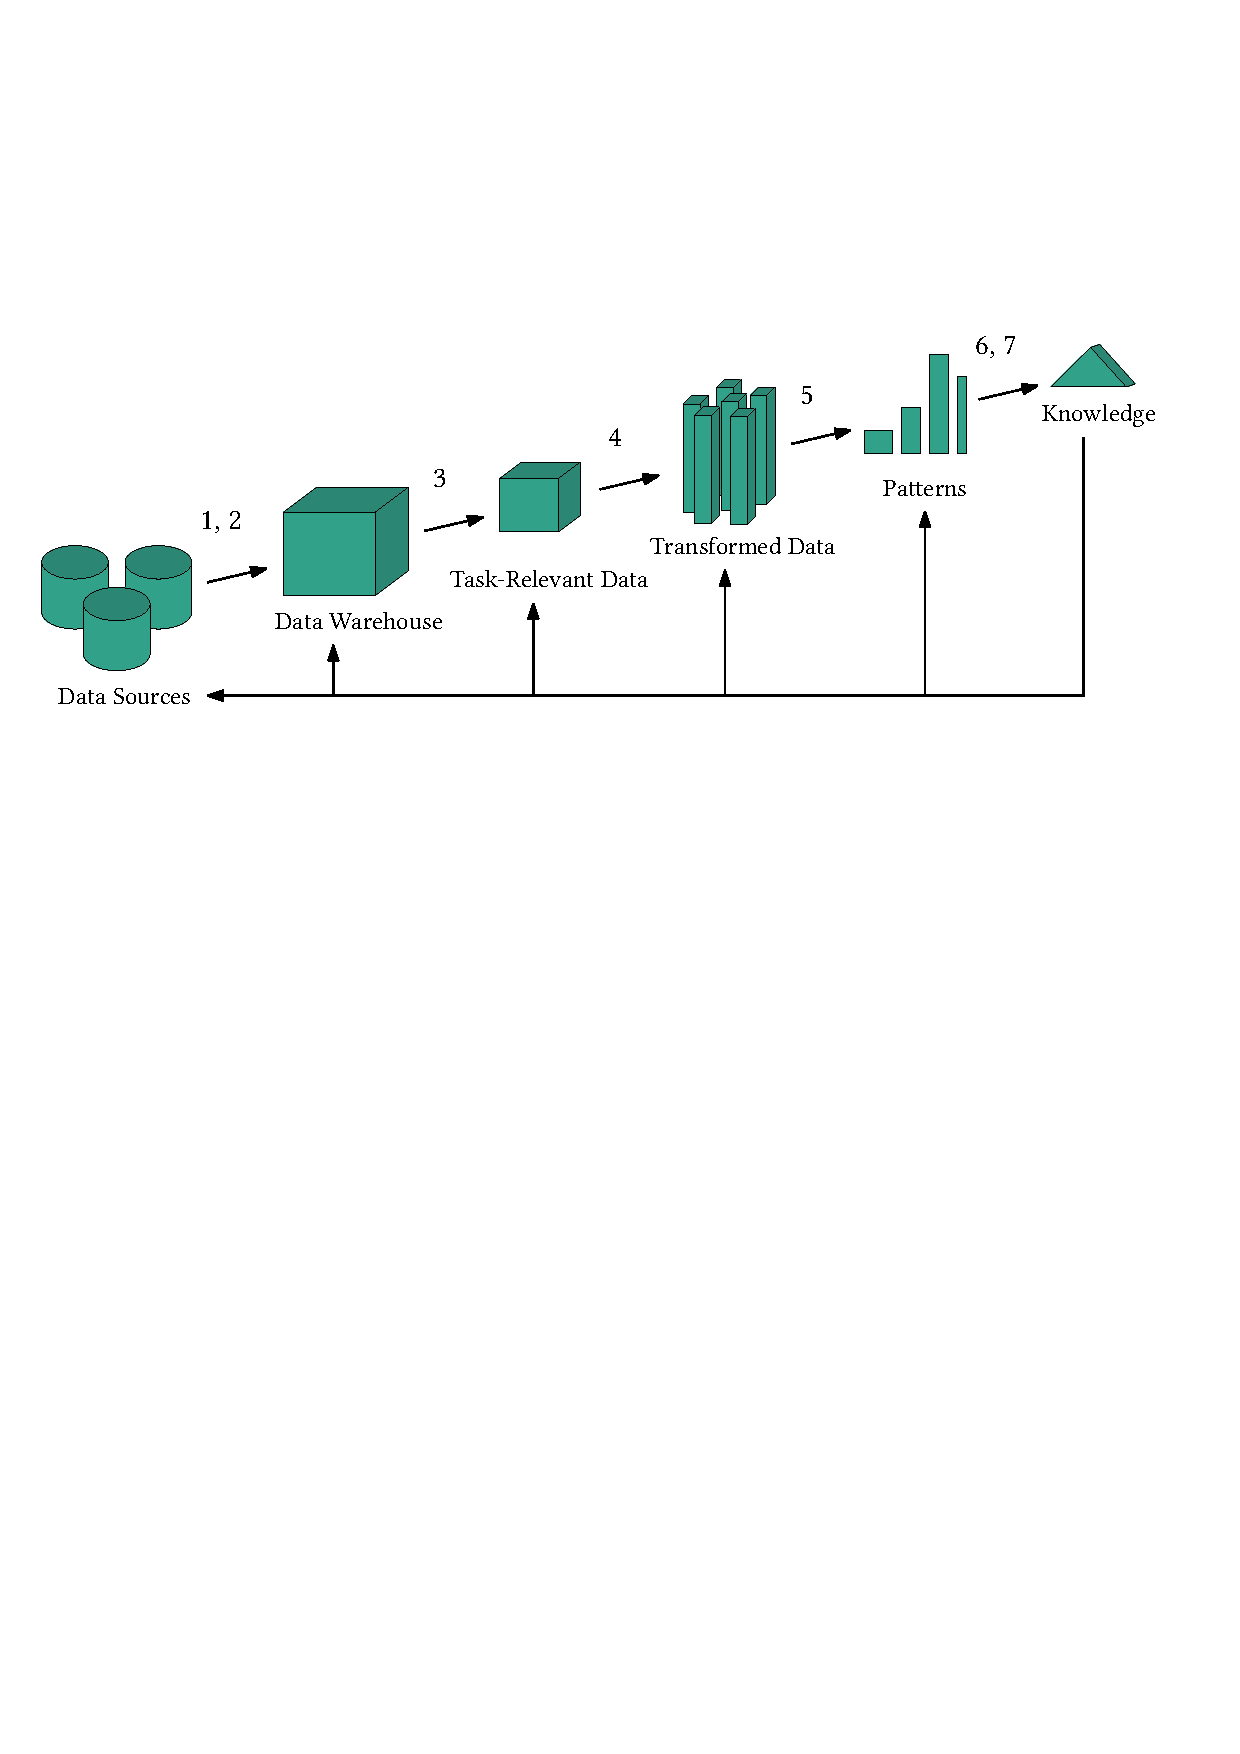
\includegraphics[width=0.95\textwidth]{part1-figures/kdd-compressed.pdf}
	\caption{\acrfull{KDD}, according to \cite{DBLP:books/mk/HanKP2011}.}
	\label{fig:KDD}
\end{figure} 

As we can see, Data Mining also refers to the core step of this process (Step 5). The literature uses the term Data Mining interchangeably with \gls{KDD}, perhaps for conciseness \cite{DBLP:books/mk/HanKP2011}. In turn, the community usually describes Data Mining as a discipline at the frontier of multiple fields: Database Management, Artificial Intelligence, Machine Learning, Pattern Recognition, Data Visualisation. In this dissertation, we refer to Data Mining or Knowledge Discovery as the whole process and leave the debate on the semantic differences w.r.t.\ Machine Learning, Data Science, etc., to the literature \cite{DBLP:books/aw/TanSK2005, Friedman97datamining}.

Researchers have examined every step of the process, and a wide range of methods is now available to extract patterns from data. 
%Note: At this point, we could have examples of for what Data Mining is useful for (but we have this in abstract now so I guess it's good enough)
However, Data Mining remains challenging under certain circumstances. In particular, when (1) the data is high-dimensional, i.e., it has many attributes, and when (2) the data comes as a stream. These two problems have raised the interest of the research community for years \cite{DBLP:journals/sadm/ZimekSK12,DBLP:books/sp/Aggarwal2013,DBLP:journals/ijon/Ramirez-Gallego17,DBLP:journals/pai/Gama12}. While the literature separately addressed them to some extent, the intersection of both has received less attention. For example, recent clustering  \cite{DBLP:journals/csur/SilvaFBHCG13,DBLP:books/daglib/0030859,DBLP:journals/jcst/AminiTS14,DBLP:journals/ijon/WuLH12} or prediction  \cite{DBLP:conf/ijcai/TanTL11,DBLP:conf/aaai/WangRNBMX17,DBLP:journals/sadm/ZimekSK12,DBLP:conf/dasfaa/AssentKBS12,DBLP:conf/icdm/SatheA16,DBLP:conf/sdm/ChenSAT17} algorithms tend to tackle at most one of those aspects: either high-dimensionality restricted to static data, or the streaming scenario, limited to few variables. 
The difficulty is that both the high-dimensionality and the streaming setting come with distinct sets of challenges. 

Data Mining at the intersection of both problems remains mostly unaddressed \cite{DBLP:journals/sigkdd/SalehiR18}, i.e., there is a gap in the current research landscape (Figure~\ref{unexplored}). While one option is to extend or invent specific methods for high-dimensional data streams, as in \cite{DBLP:conf/icde/ZhangGW08, DBLP:conf/sdm/NtoutsiZPKK12}% see also \cite{ DBLP:conf/vldb/AggarwalHWY04,  DBLP:conf/icde/ZhangGW08, DBLP:conf/icde/CaoYWYWR14}, % DBLP:conf/ssdbm/HassaniKSS14, 10.1145/3219819.3220107
, a perhaps more general -- but not less effective -- contribution is to develop fundamental tools for Knowledge Discovery in this particularly challenging setting. 

This observation forms the starting point of our dissertation. We bridge this gap by proposing algorithms to address both sets of challenges. We start with a fundamental task: dependency estimation. We show that, combined with efficient monitoring techniques, our algorithms support further Knowledge Discovery in high-dimensional data streams.

\begin{figure}
	\centering
	\begin{tikzpicture}[thick]
	
	\begin{scope}
	\clip (2.5,2) circle (2.5cm);
	\fill[pattern=crosshatch, pattern color=uiucred] (6.5,2) circle (2.5cm);
	\end{scope}
	\draw (2.5,2.25) node { High};
	\draw (2.5,1.75) node { Dimensionality};
	\draw (2.5,2) circle (2.5cm);
	
	\draw (6.5,2) circle (2.5cm);
	\draw (6.5,2.25) node { Data};
	\draw (6.5,1.75) node { Streams};
	
	\end{tikzpicture}
	\caption{A gap in the Data Mining research landscape.}
	\label{unexplored}
\end{figure}

In the remaining of this chapter, we detail the challenges associated with high-dimensionality and data streams. Then, we show that the task of dependency estimation is critical to most Data Mining applications and present our running use case: the \acrshort{Bioliq} power plant. Finally, we detail our contributions and the outline of this dissertation.  

\subsection{Challenges of High-Dimensionality}
\label{challenges:highdimensionality}

When the data is high-dimensional, several effects, summarised as the \textit{curse of dimensionality} \cite{bellman1957}, bog down the performance of traditional statistical approaches \cite{DBLP:conf/icdt/BeyerGRS99}. 

A linear increase in the number of dimensions in the euclidean space leads to an exponential increase in volume. The space becomes extremely sparse, and the distances between each pair of points converge to the same value. This effect is known as \textit{distance concentration}. \cite{DBLP:conf/icdt/BeyerGRS99} showed that, under broad conditions, the probability that the minimum $\mathcal{D}_{\text{min}}^n$ and the maximum distance $\mathcal{D}_{\text{max}}^n$ differ by a factor smaller than $1 + \epsilon$ converges to $1$ as the number of dimensions $n$ increases, i.e., 
\begin{align}
\lim_{n \rightarrow \infty} \Pr\left[\mathcal{D}_{\text{max}}^n \leq (1 + \epsilon) \cdot \mathcal{D}_{\text{min}}^n\right] = 1, \quad \forall \epsilon > 0. 
\end{align} 

Figure~\ref{fig:cod} illustrates this via simulation. We report the maximum, average and minimum euclidean pairwise normalised distances within $100$ \textit{i.i.d.} observations in $\mathcal{U}[0,1]$. We average the results over $1000$ independent trials; The coloured areas show the standard deviation. As we can see, the distances converge as $n$ increases. Thus, in high-dimensional spaces, observations tend to be equally far from each other. The performance of most Data Mining algorithms, which rely on local neighbourhoods, drastically decreases.  

\begin{figure}
	\centering
	\subfigure[The \textit{distance concentration} effect]{
		\label{fig:cod}
		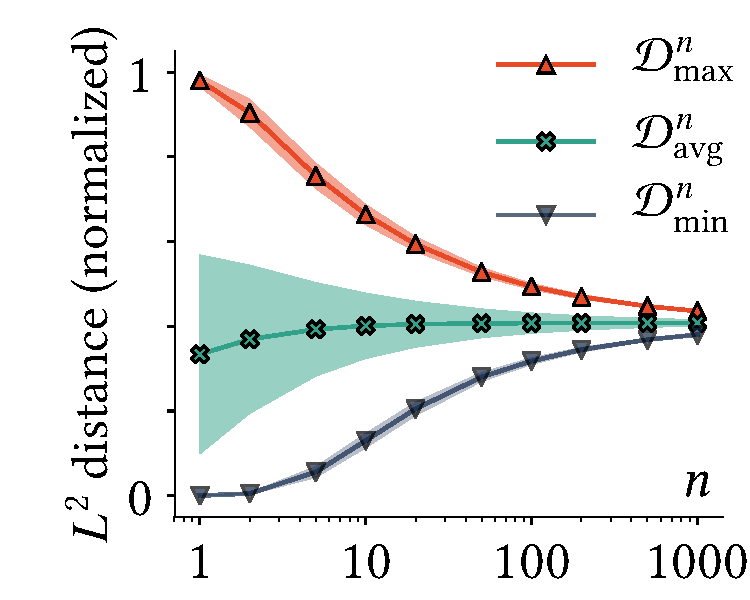
\includegraphics[width=0.36\linewidth]{part1-figures/cod_illustration-compressed.pdf}
	}
	\hfill
	\subfigure[Number of pairs]{
		\label{fig:cod_pairs}
		\begin{tikzpicture}[thick]
		\begin{axis}[width=0.34\textwidth, height=0.35\textwidth, axis lines=middle,xlabel=$n$,enlargelimits,
		scaled y ticks={base 10:-3}] 
		\addplot[domain=2:100, color=uiucblue] {x*(x-1)/2} node[left]{$f(n) = \frac{n \cdot (n-1)}{2}$};
		
		\end{axis}
		\end{tikzpicture}}
	\hfill
	\subfigure[Number of subspaces]{
		\label{fig:cod_subspaces}
		\begin{tikzpicture}
		\begin{axis}[width=0.34\textwidth, height=0.35\textwidth, axis
		lines=middle,xlabel=$n$,enlargelimits] 
		\addplot[domain=2:20, color=uiucred] {2^x - 1} node[left]{$g(n) = 2^n - 1$};
		\end{axis}
		\end{tikzpicture}}
	\caption{Illustration of the effects of the \textit{curse of dimensionality}.}
	\label{fig:searchspace}
\end{figure}
%Note: "Conventional method such as Kernel Density Estimation (KDE) performs poorly for high-dimensionaldata (d >3)." -> Nonparametric Density Estimation for High-Dimensional Data - Algorithms and Applications (Zhipeng Wang∗and David W. Scott)
% Source saying that density estimation in high-dimensional space does not work -> Scott (Multivariate Dependency Estimation, page 202)

A common workaround consists in restricting the analysis to small sets of attributes (subspaces) of interest, e.g., via \textit{dimensionality reduction} methods. 
However, \textit{dimensionality reduction} also is challenging: the number of pairs for a number $d$ of attributes is $\frac{n \cdot (n-1)}{2}$ for symmetric measures (Figure~\ref{fig:cod_pairs}), while the number of subspaces is $2^n - 1$ (Figure~\ref{fig:cod_subspaces}). As a result, they grow quadratically/exponentially with $n$, so that, even for a moderate amount of attributes, one cannot afford to investigate each attribute pair or subspace. 

For example, with $20$ attributes, the number of subspaces is already more than one million (Figure~\ref{fig:cod_subspaces}).
\cite{DBLP:books/sp/Aggarwal2013} famously compared the task of finding a pattern (e.g., an outlier) in high-dimensional spaces to that of searching for a needle in a haystack, while the haystack is one from an exponential number of haystacks. Subspace search methods, such as \cite{DBLP:conf/sdm/BohmKMNV13, DBLP:conf/bigdataconf/NguyenMB13, DBLP:conf/icde/KellerMB12, DBLP:journals/ijdsa/TrittenbachB19}, efficiently solve this problem to some extent. 

%The problem is that patterns, such as outliers, may only be visible within a few of those subspaces \cite{DBLP:conf/icde/KellerMB12}. 

We refer to \cite{DBLP:books/lib/HastieTF09} for further illustrations of the effect of the \textit{curse of dimensionality} and to \cite{DBLP:journals/sadm/ZimekSK12} for a discussion centred on outlier detection. 

\subsection{Challenges of Data Streams}
\label{challenges:datastreams}

In the real world, data often is a stream, i.e., data is collected online and may evolve in unforeseeable ways. In this setting, static approaches are ineffective \cite{DBLP:journals/pai/Gama12} because of changes in the data generation, characterised by a phenomenon known as \textit{concept drift}.

Thus, patterns are meaningful only in the right time context. For example, in Figure~\ref{fig:drift}, an observed outlier at time $T=1$ might not be relevant any more at time $T=2$ and vice-versa. Next, the scale of this time context also is unknown. In broader time contexts, e.g., $T=\{1,2,3\}$, the outliers may not be visible as such.

\begin{figure}
	\centering
	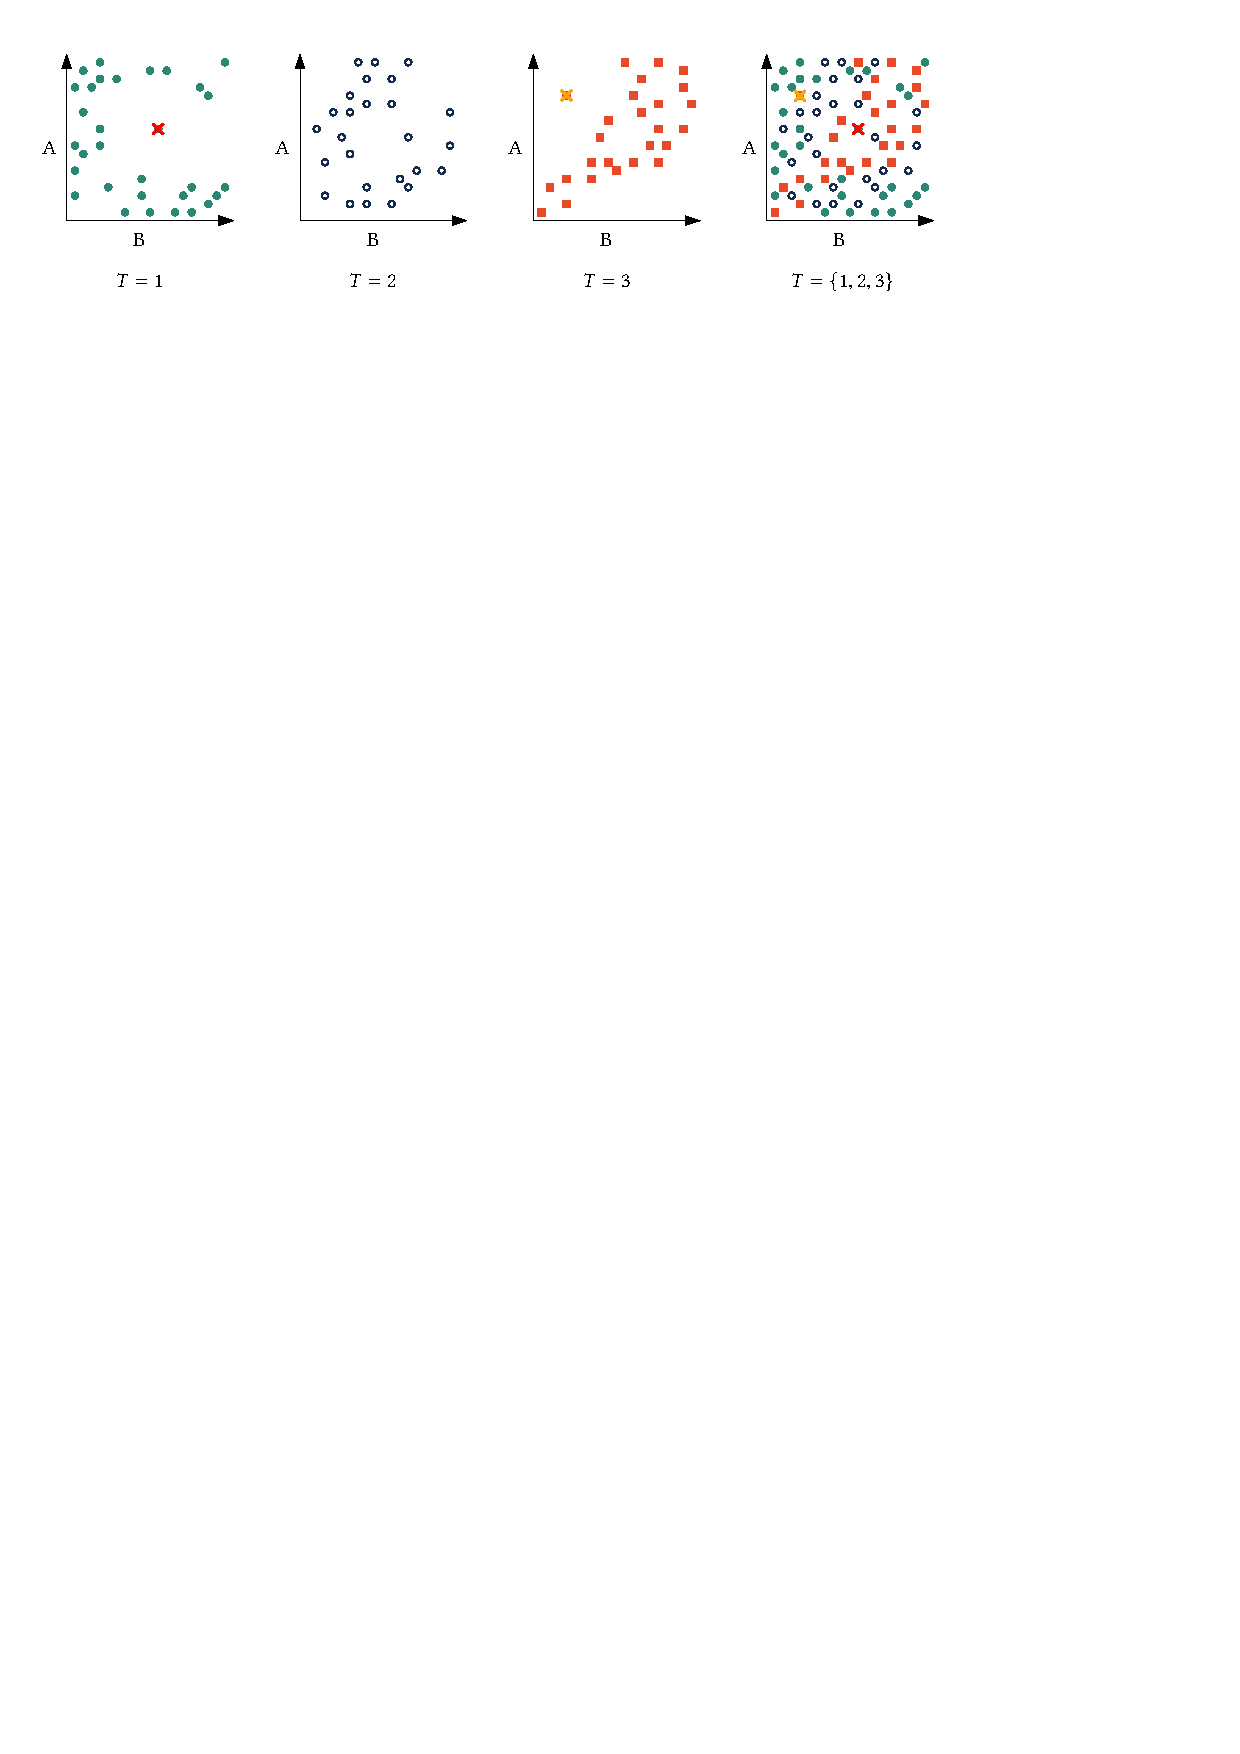
\includegraphics[width=1.0\textwidth]{part1-figures/time_example-compressed.pdf}
	\caption{Concept drift -- Patterns are only visible in their local context.}\label{fig:drift}
\end{figure} 

Data streams are subject to various types of \textit{concept drifts} \cite{DBLP:conf/ictai/BarddalGE15}, which can vary in speed and intensity and may also have seasonal components. 
The streaming nature of the data constrains system design in several ways, laid out by \cite{doi:10.1198/1061860032544} as follows:  
\begin{itemize}[noitemsep]
	\item \hypertarget{C1}{\textbf{Efficiency (C1):}}  The system must spend a short constant time and a constant amount of memory to process each incoming record.
	\item \hypertarget{C2}{\label{C2} \textbf{Single Scan (C2):}} The system may perform at most one scan over the data since access to past observations is often unavailable or impractical. 
	\item \hypertarget{C3}{\textbf{Adaptation (C3):}} Whenever the data distribution changes over time, the system must adapt, e.g., by forgetting outdated information.
	\item \hypertarget{C4}{\label{C4} \textbf{Anytime (C4):}} The system must be available at any point in time, with an output ideally equivalent (or nearly identical) to the one of a non-streaming system, operating without the streaming constraints. 
\end{itemize}   
The streaming scenario is particularly challenging because one needs to monitor the evolution of data. Data Mining algorithms must integrate an adequate forgetting mechanism to discard obsolete information and monitor the stream.

%Additionally, the high-dimensionality challenges the efficiency and effectiveness of streaming algorithms. In the end, the computational effort of existing methods generally is too high to allow for their deployment in real-time.

Furthermore, streams often consist of observations with various types, e.g., numerical, ordinal, or categorical. Such data sources are known as \textit{Heterogeneous Data Streams} \cite{DBLP:conf/icdm/YangZ06}. \cite{DBLP:journals/cim/DitzlerRAP15} identified mining from heterogeneous data as one of the most challenging problems of Data Mining. Thus, \textit{heterogeneity} adds up to the list of constraints above:
\begin{itemize}
	\item \hypertarget{C5}{\label{C5} \textbf{Heterogeneity (C5)}}: The system must handle not only numerical types but ideally all data types such as strings, categories, ordinal values. 
\end{itemize} 
The main challenge is to provide Data Mining techniques that can cope both with the streaming constraints and high-dimensionality -- our goal in this dissertation.  

\subsection{The Central Role of Estimating Dependency}
\label{sec:centralrole}

Dependency estimation is a fundamental technique in Data Mining \cite{DBLP:journals/tkde/ChenHY96} and consists of quantifying the strength of the statistical relationship between attributes, based on the available observations. It helps to find the relevant variables for the task at hand, which leads to a better understanding of data and improves both the runtime and the outcomes of downstream mining tasks, e.g., classification, outlier detection, or clustering.

To this end, dependency estimators such as the \textit{Pearson correlation coefficient}, or \textit{mutual information} \cite{DBLP:journals/bstj/Shannon48} as a non-linear counterpart, are perhaps the most well-known examples. Dependency estimation techniques are a building block of many Data Mining approaches, and play a role at every step of the process (see Figure~\ref{fig:KDD}), for example:
\begin{itemize}[noitemsep]
	\item \gls{EDM} \cite{DBLP:books/wi/DasuJ03, DBLP:journals/sigkdd/AssentKMS07, DBLP:conf/ieeevast/TatuMFBSSK12} is fundamental for \textbf{Data Cleaning} and \textbf{Data Integration}. \gls{EDM} reveals structures in the data, e.g., artefacts and inconsistencies that one should clean, or relevant attributes to integrate before subsequent analysis. Dependency estimators \cite{DBLP:journals/sigkdd/ParsonsHL04, DBLP:conf/vldb/ZhuS02, DBLP:conf/sigmod/MayfieldNP10} are a characteristic tool of \gls{EDM} to discover such structures.  
	\item Filtering out the attributes irrelevant for the task at hand is key to deal with high-dimensionality. \textit{Feature Selection} \cite{DBLP:journals/jmlr/GuyonE03} methods are critical for \textbf{Data Selection} and heavily rely on dependency estimators \cite{DBLP:journals/pami/PengLD05, DBLP:journals/tkde/HallH03, DBLP:journals/eswa/BennasarHS15, DBLP:journals/pr/LiuSLZ09}. 
	\item \textbf{Data Transformation}, also known as \textit{Feature Engineering}, consists in transforming the data into an adequate format, and possibly enhancing the original data with additional features. Dependency estimates can be used as feature to improve the results of downstream analysis \cite{DBLP:conf/vldb/ZhuS02, DBLP:journals/jmlr/Torkkola03, DBLP:conf/icml/YuanH09, DBLP:conf/eenergy/VollmerETBKB19}. 
	\item Numerous \textbf{Data Mining} algorithms, e.g., clustering \cite{DBLP:conf/sdm/BohmKMNV13, DBLP:conf/bigdataconf/NguyenMB13} or outlier detection \cite{DBLP:conf/icde/KellerMB12, DBLP:journals/ijdsa/TrittenbachB19} algorithms, intrinsically rely on dependency estimation. 
	\item Finally, dependency estimation also helps for \textbf{Pattern Evaluation} and \textbf{Knowledge Representation}. For example, \cite{DBLP:journals/pvldb/GebalyAGKS14, DBLP:journals/debu/GebalyFGKS18, DBLP:conf/ssdbm/VollmerGBS19} leverage \textit{mutual information} to evaluate and represent rules learned from data. 
\end{itemize}
Also, dependency estimation is essential in high-dimensional data streams, because most tasks are \textit{unsupervised}, i.e., the nature of objects (e.g., inlier/outlier) may be unknown or revealed only with some latency \cite{DBLP:journals/cim/DitzlerRAP15}. Such tasks %, e.g., clustering or outlier detection, 
typically boil down to discovering structures in data, which in turns often relies on dependency estimation. 

However, there are -- to our knowledge -- no dependency estimation technique suitable for high-dimensional data streams. The existing methods are impractical, because they either are inefficient or restricted to the bivariate case. 

Next, there exists no efficient solution to maintain an overview of statistics (e.g., dependency estimates) concerning numerous subspaces. One often has no choice but to recompute the measures of interest periodically, which can be very expensive. While there exist a few monitoring techniques \cite{DBLP:conf/vldb/ZhuS02, DBLP:conf/sdm/BifetG07}, they can either (1) only monitor a single statistic or (2) only support a specific estimator, and do not generalise beyond. 

Data Mining algorithms currently are unable to leverage dependency estimation in high-dimensional data streams. Therefore, developing new methods for dependency estimation and monitoring in this setting is much needed.
%Note: Maybe talk about multivariate dependency estimation. Go into the problems of the existing dependency estimators. Have a small paragraph about this.

%Also, dependency estimation is even more critical in the streaming setting, because problems typically are \textit{unsupervised}. Unsupervised learning refers to a branch of Machine Learning, in which no ground truth, i.e., category labels or clusters, is known beforehand. In essence, \textit{unsupervised} methods boil down to discovering structure in the data and make heavy use of dependency estimation techniques.  
%For example, the problem of detecting anomalies from a large number of sensors in a factory should be considered \textit{unsupervised}: It is apriori unknown what an anomaly looks like before it occurs. Since anomalies are rare and need to be prevented, there are no or only very few examples available from which one could learn. 
%So far, an overwhelming majority of the literature focused on \textit{supervised} settings. Let us think a typical \textit{supervised} learning problem formulation: Given a set of training objects, each of them known to belong to one class among $N$ specific ones, learn a model to predict the class of future objects. Such a problem does not fit the streaming setting, because the characteristics of classes may change over time (i.e., because of \textit{concept drift}), making the strict definition of classes meaningless. Next, the actual label of objects may be unknown or revealed only with some latency \cite{DBLP:journals/cim/DitzlerRAP15}. 

\subsection{The \acrshort{Bioliq}\texorpdfstring{\textsuperscript{\textregistered}}{} Power Plant: A Real-World Use Case}
\label{sec:bioliqexample}

%Identifying patterns in high-dimensional streams is extremely useful in many scenarios: The prompt extraction of knowledge from data may lead to an increase of production volumes, or the avoidance of additional costs. 

Throughout this dissertation, we illustrate our results against a real-world use case: the \acrshort{Bioliq} power plant. %\footnote{\url{https://www.bioliq.de}}. 
In a nutshell, the goal of the \gls{Bioliq} project is to develop the process chain for producing fuels from biomass at an industrial scale. The \gls{Bioliq} plant provides real-world data that we use to motivate and validate our research. 

We focus in particular on the first part of the \gls{Bioliq} process: the fast pyrolysis, which takes place in the `Bioliq I' pilot plant in the surroundings of Karlsruhe \cite{pfitzer2016fast}. We show in Figure~\ref{fig:bioliq_schematics} a simplified representation of the process. The following example illustrates the importance of monitoring statistics, such as dependency estimates, at \gls{Bioliq}:
\begin{figure}
	\centering
	\hfill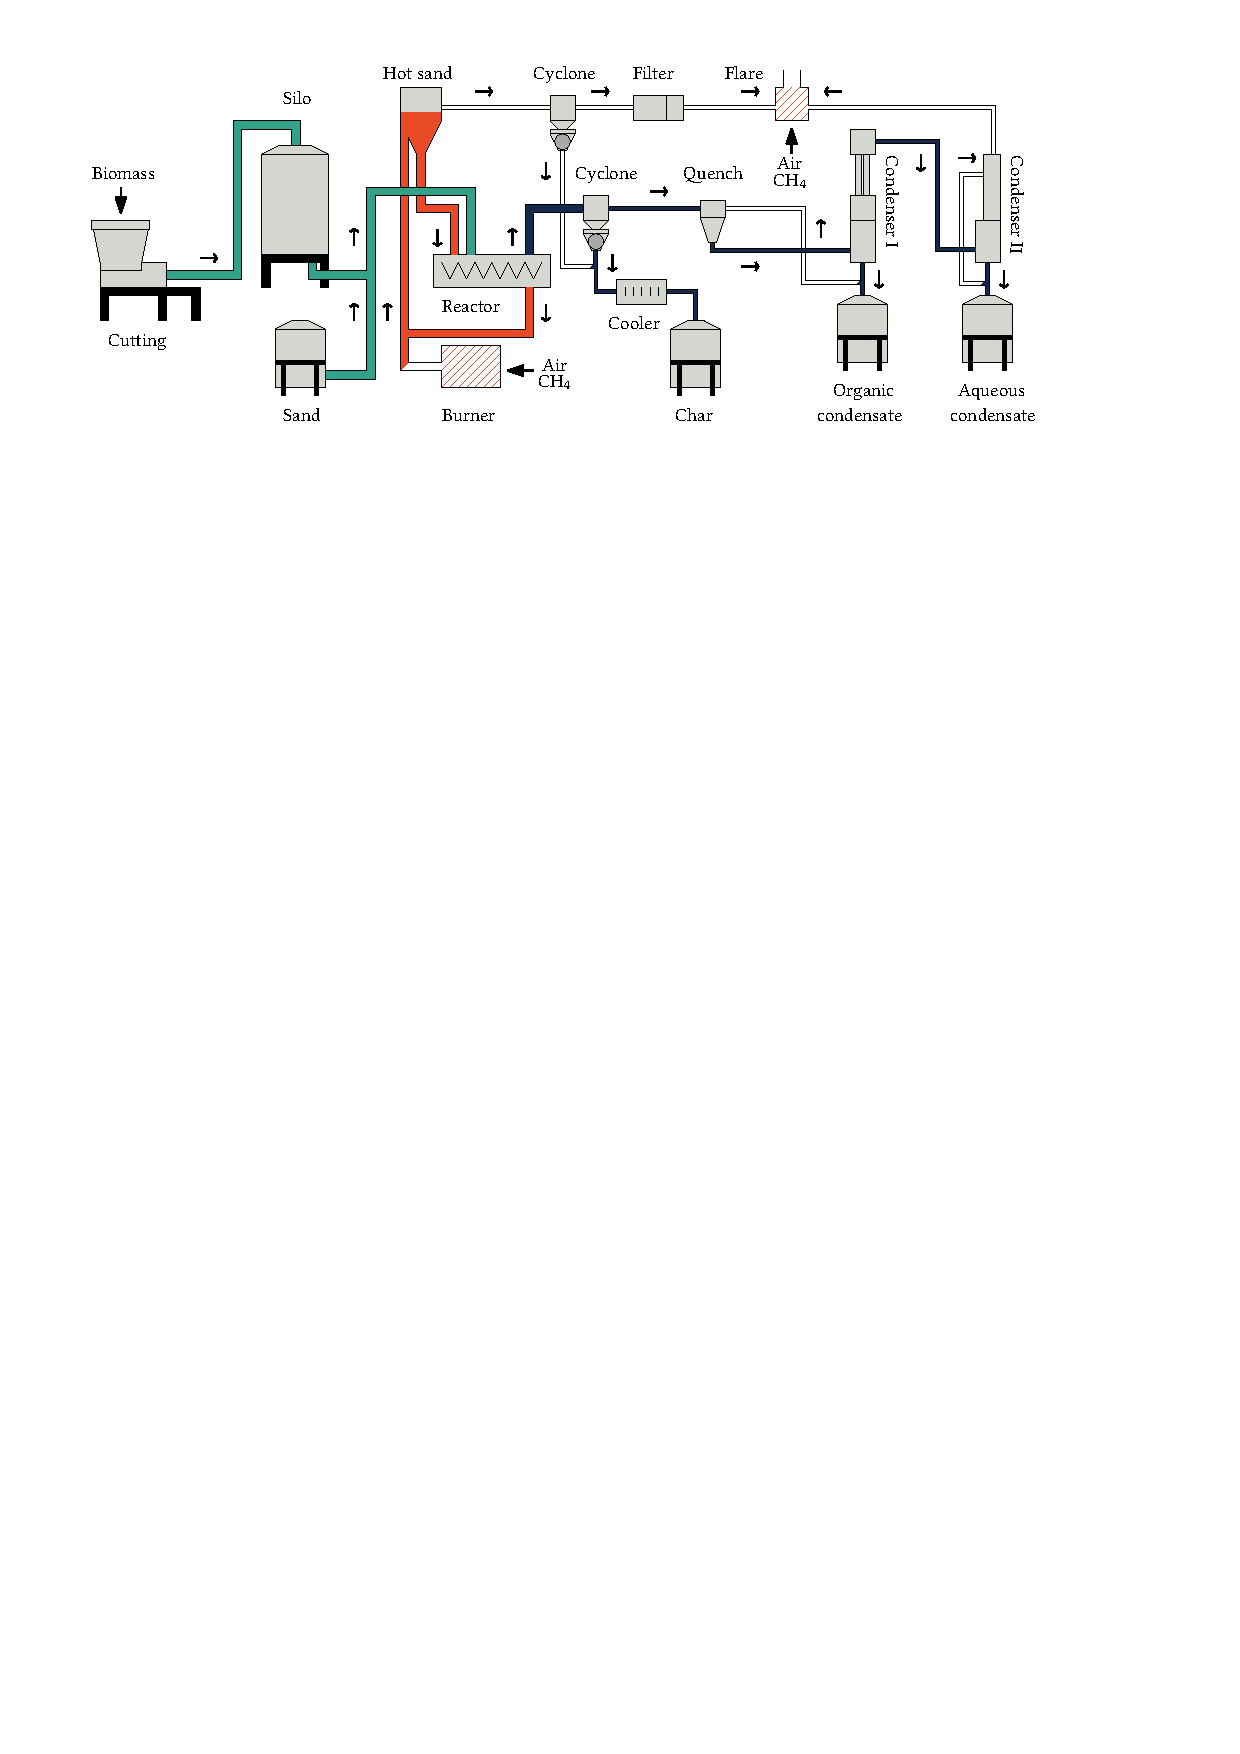
\includegraphics[width=0.95\textwidth]{part1-figures/bioliq_schematics_2-compressed.pdf}\hfill
	\vspace{0.3cm}
	\hfill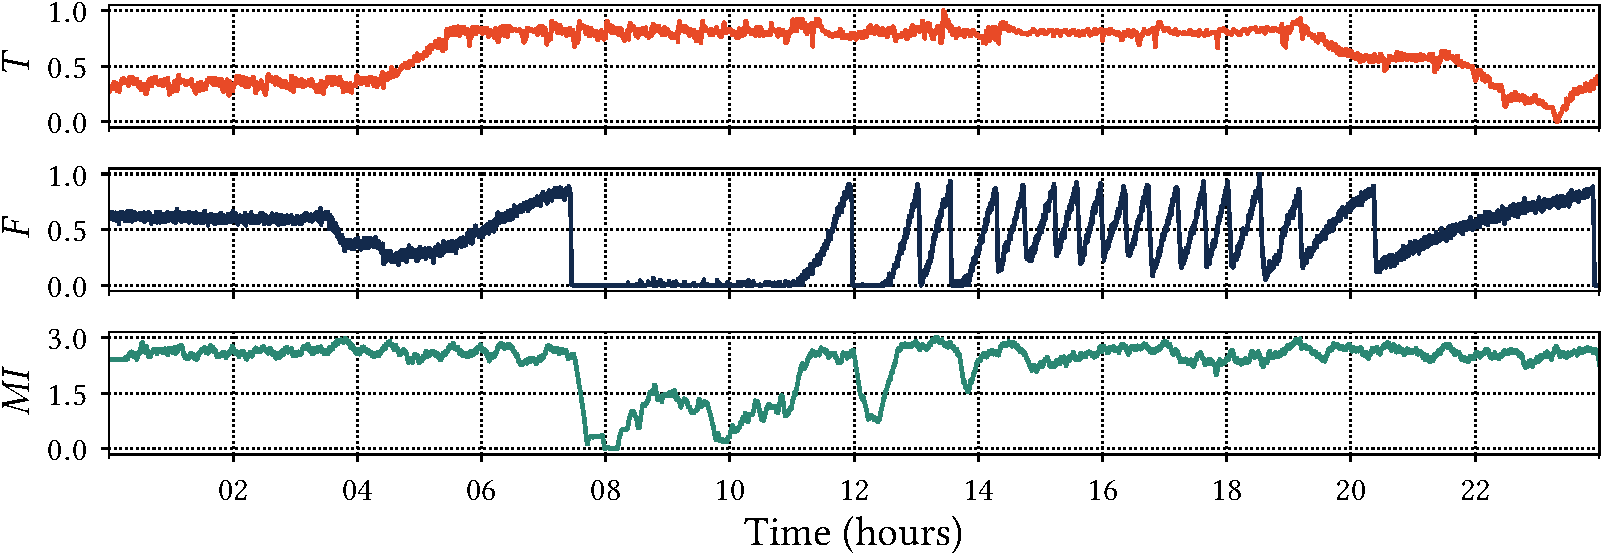
\includegraphics[width=0.95\textwidth]{part1-figures/bioliq_prep_s-crop-compressed.pdf}\hfill
	\caption{Schematics of the \acrshort{Bioliq} fast pyrolysis and monitoring example.}\label{fig:bioliq_schematics}
\end{figure}

\begin{example}[Monitoring at \acrshort{Bioliq}]
	Let us observe a 24-hours measurement period of two sensors at \gls{Bioliq}: $T$ is the temperature in the reactor, and $F$ is the filling level of the flue gas cyclone connected to its output. We report the \gls{MI} between $T$ and $F$ at any time over the last 15 minutes. 
	In the beginning, the reactor heats up to its operational temperature. The material introduced leads to the exhaustion of flue gas, stored temporarily in the cyclone for further processing. The  \gls{MI} between the two streams suddenly drops from 2.5 bits to 0 at 7:45. The cyclone does not seem to operate as it should, i.e., as in the later timespan between 12:00 and 20:00. The data indicates an interruption in production. Such interruptions can become very costly if unnoticed. Thus, the careful monitoring of plant elements is essential, as drifting dependencies might indicate abnormal events \cite{DBLP:journals/tim/Hashemian11}. 
	%See \url{https://www.bioliq.de} for more information about the Bioliq process.
\end{example}
%Note: I am not sure that this is very conclusive at this point 
%We discuss here one possible use case, but the Bioliq plant provides numerous similar examples. The Bioliq plant capture typical use cases from the field of \textit{predictive maintenance}, which represent a primary application of our research.  
%Maybe add a small paragraph saying what the bioliq data is made of. (attributes... etc) and that we will release it. 

\section{Contributions}

The goal of this dissertation is to address the challenges of Data Mining w.r.t. high-dimensionality and streaming data. To this end, we first focus on fundamental problems of Data Mining: estimating dependency and monitoring. Then, we show how our new methods help to address Knowledge Discovery in high-dimensional data streams. We organise our contributions around the three following research questions: 

\begin{itemize}[noitemsep]
	\item \hypertarget{Q1}{\textbf{Q1 (Estimating Dependency):}} The increasing number of dimensions and observations challenge dependency estimation. How to estimate dependency in high-dimensional data streams efficiently and effectively? 
	\item \hypertarget{Q2}{\textbf{Q2 (Monitoring):}} By nature, data streams are infinite and may evolve, so the relationship between variables might change. How can we keep track of the evolution of statistics (e.g., dependency estimates) in streams with high-dimensionality?  
	\item \hypertarget{Q3}{\textbf{Q3 (Knowledge Discovery):}} We see the answer to \hyperlink{Q1}{\textbf{Q1}} and \hyperlink{Q2}{\textbf{Q2}} as fundamental to extract knowledge from high-dimensional streams. Thus, we ask: how to leverage our contributions to mine patterns (e.g., anomalies) in this setting?  
\end{itemize} 

To deal with \hyperlink{Q1}{\textbf{Q1}}, we propose a list of desirable features an estimator must ideally fulfil for high-dimensional data streams. Then, we introduce \gls{MCDE}, a framework that quantifies multivariate dependency as the average statistical discrepancy between marginal and conditional distributions, via Monte Carlo (MC) simulations. \gls{MCDE} handles heterogeneity by leveraging three statistical tests: the Mann-Withney U, the Kolmogorov-Smirnov and the Chi-Squared test. We determine a lower bound for the quality of our estimates, which only depends on the number of MC simulations. Such bound allows users to trade estimation accuracy for a computational advantage. We demonstrate that \gls{MCDE} goes beyond the current state of the art regarding dependency estimation by meeting all the features defined previously. Finally, we show against our real-word use case (\gls{Bioliq}) that \gls{MCDE} can discover useful patterns in high-dimensional data streams. We recently published those results in \cite{DBLP:conf/ssdbm/FoucheB19, DBLP:conf/ssdbm/FoucheBMKB20}. 

Concerning \hyperlink{Q2}{\textbf{Q2}}, we propose to formulate the problem of monitoring statistics in high-dimensional data streams as a \gls{MAB} problem. We find that our setting requires to extend the existing models, and call our extension the \gls{S-MAB}. We propose a new algorithm based on \gls{TS}, with strong theoretical guarantees and excellent empirical performance. Furthermore, we combine our algorithm with \gls{ADWIN}, a state-of-the-art change detector, to deal
with non-static environments. We illustrate the benefits of our contribution using synthetic data, as well as data from our real-world use case. We published our findings in \cite{DBLP:conf/kdd/FoucheKB19}. 

Finally, we address \hyperlink{Q3}{\textbf{Q3}} by exploiting synergies between our previous contributions. We show that, by combining the ideas behind \gls{MCDE} and \gls{S-MAB}, we can facilitate the search for subspaces in data streams. We introduce a new algorithm, \gls{SGMRD}, and show that \gls{SGMRD} leads to state-of-the-art performance for Knowledge Discovery tasks, such as outlier detection. Then, we propose a new method, \gls{kj-NN}, to detect outlying documents within large text corpora. Those contributions are featured here \cite{DBLP:conf/ssdbm/FoucheMGZBH20, DBLP:conf/review/FoucheKB20}.

%All in all, the goal of this dissertation is to establish fundamental tools for knowledge discovery in high-dimensional data streams. We propose efficient methods for estimating and monitoring dependency, which plays a central role in most Data Mining approaches.

\section{Outline}

We structure the rest of this dissertation as follows: 

\begin{itemize}
	\item Chapter \ref{chapter:preliminaries} is a joint introduction to our contributions w.r.t. \hyperlink{Q1}{\textbf{Q1}}, \hyperlink{Q2}{\textbf{Q2}} and \hyperlink{Q3}{\textbf{Q3}}. We introduce a set of desirable features for dependency estimators in high-dimensional data streams and formulate the problem of monitoring in high-dimensional data streams as a \acrfull{MAB} problem. Then, we discuss our applications to Knowledge Discovery in high-dimensional data streams.
	\item Chapter \ref{chapter:relatedwork} presents the related work concerning each of our contributions. 
	\item Part \ref{partII} focuses on \hyperlink{Q1}{\textbf{Q1}}. In Chapter \ref{chapter:MCDE}, we present a new framework for dependency estimation: \acrfull{MCDE}. 
	\item Part \ref{partIII} answers \hyperlink{Q2}{\textbf{Q2}}. Chapter \ref{chapter:S-MAB} introduces the \acrfull{S-MAB} algorithms, our solution to monitor high-dimensional data streams. 
	\item Part \ref{partIV} deals with \hyperlink{Q3}{\textbf{Q3}}. Chapter \ref{chapter:subspacesearch} introduces a general method for Subspace Search in Data Streams, named \acrfull{SGMRD}. Chapter \ref{chapter:textoutlier} presents a new algorithm, \acrfull{kj-NN}, to detect outlying documents within large text corpora.
	\item Part \ref{partV} concludes by summarising the outcome of this dissertation in Chapter \ref{chapter:summary}, while Chapter \ref{chapter:futurework} provides an outlook on future work and research directions.  
\end{itemize}

The content relevant to this dissertation extends beyond the scope of this document. Readers may find complementary information about Bioliq in the literature \cite{pfitzer2016fast} and the official website of the Bioliq project: 
\begin{itemize}
	\item Bioliq: \url{https://www.bioliq.de}
\end{itemize}

Furthermore, we systematically release our source code, data and experiments via open-source platforms, under the GNU Affero General Public License version 3 (\href{https://www.gnu.org/licenses/agpl-3.0.en.html}{AGPLv3}): 

\begin{itemize}
	\item \gls{MCDE}: \url{https://github.com/edouardfouche/MCDE-experiments}; \url{https://github.com/edouardfouche/MCDE}; \url{https://github.com/edouardfouche/MCDE-extended}
	\item \gls{S-MAB}: \url{https://github.com/edouardfouche/S-MAB}
	\item \gls{SGMRD}: \url{https://github.com/edouardfouche/SGMRD} 
	\item \gls{kj-NN}: \url{https://github.com/edouardfouche/MiningTextOutliers} 
\end{itemize}

See also the related entries on the author's website  (\url{https://edouardfouche.com}) and the sources of this document (\url{https://github.com/edouardfouche/phd-thesis}), under the Creative Commons Attribution-ShareAlike 4.0 International License (\href{https://creativecommons.org/licenses/by-sa/4.0/}{CC BY-SA 4.0}).

\chapter{Preliminaries}
\glsresetall
\label{chapter:preliminaries}

This chapter is a joint introduction to our core contributions. % and bases on several publications associated with this dissertation, in particular: \cite{DBLP:conf/ssdbm/FoucheB19, DBLP:conf/ssdbm/FoucheBMKB20, DBLP:conf/kdd/FoucheKB19, DBLP:conf/ssdbm/FoucheMGZBH20, DBLP:conf/review/FocuheKB20}. 
We describe the underlying motivations and the notation for our work. %, organised around our three main topics: Estimating Dependency, Monitoring and Knowledge Discovery.

\section{Estimating Dependency}

\subsection{Motivations}  

The discovery of relationships between attributes is fundamental to many Data Mining applications, e.g., Feature Selection \cite{DBLP:journals/pami/PengLD05}, Clustering \cite{DBLP:conf/sdm/BohmKMNV13} or Outlier Detection \cite{DBLP:conf/icde/KellerMB12}, and it is a prominent topic in the database community \cite{DBLP:journals/tkde/ChenHY96, DBLP:conf/vldb/ZhuS02, DBLP:journals/tkde/HallH03}. 

One typically estimates the strength of a relationship by estimating the `dependence' among the attributes of a subspace. To do so, one often leverages well-known `dependency estimators' such as the Pearson correlation coefficient (also known as \textit{correlation}), or \gls{MI} \cite{DBLP:journals/bstj/Shannon48} as a non-linear counterpart. 

Dependency estimation not only plays a central role in Data Mining -- as we discussed in Section~\ref{sec:centralrole} -- but also delivers useful information per se: knowing the relationship between attributes helps to predict and understand certain outcomes. 

\glsunset{Bioliq}
For instance, knowing that weight and arterial pressure correlate with the odds of contracting certain diseases may guide physicians, when predicting whether a patient will become sick within a year or not. Dependency may also reflect natural physio-chemical relationships, say, between the temperature and pressure of a fluid in a pipe. When dependency changes, it either means that the system's state is transitioning, e.g., the fluid solidifies, or that equipment deteriorates, e.g., there is a leak. Fluctuations of dependency often reflect changes in the stream, i.e., the dependency matrix delivers information about the state of a system. This applies, for example, to the \gls{Bioliq} plant (Figure \ref{fig:bioliq_schematics}). 

However, concerning real-world settings, dependency estimation remains mostly unaddressed: data often comes as an open-ended, ever-evolving stream of sensor signals. The signals can be noisy, redundant or generated at a varying speed. In this setting, the timely detection of changes in the stream is crucial; the early discovery of anomalies can, say, facilitate predictive maintenance and yield tremendous cost savings.

Also, most dependency estimators only deal with numerical data, while the stream often consists of measurements or indicators of various types, e.g., numerical, ordinal, or categorical observations. Such data sources are known as \textit{Heterogeneous Data Streams} \cite{DBLP:conf/icdm/YangZ06}. In Section \ref{challenges:datastreams}, we reviewed the constraints associated with data streams. Naturally, addressing those constraints is a prerequisite for any algorithm operating on streams. 
%Knowledge discovery in H-DS is known as one of the most challenging problems in Data Mining  \cite{DBLP:journals/cim/DitzlerRAP15}, as we discussed previously.  

With this in mind, and orthogonally to the constraints of the streaming setting, modern dependency estimators also have their own set of requirements -- or desirable features -- that they ideally must fulfil. We describe those requirements hereafter. 
%\enlargethispage{\baselineskip}

\subsection{Requirements}

Based on our observation of the current state of the art, our first contribution is to establish the following set of requirements, that any dependency estimator must ideally satisfy:

\begin{itemize}[noitemsep]
	\item \hypertarget{R1}{\textbf{Multivariate (R1):}} Bivariate measures only apply to two entities (i.e., variables, vectors). Estimating the dependency between more than two entities is useful as well, but existing attempts to generalise bivariate measures lack efficiency or effectiveness. %\cite{DBLP:conf/aaai/WangRNBMX17}. 
	
	\item \hypertarget{R2}{\textbf{General-purpose (R2):}} Estimators should not restrict to specific types of dependencies. Otherwise, they may miss relevant attribute relationships. Existing multivariate estimators are typically limited to, say, monotonous or functional dependencies. 
	
	\item \hypertarget{R3}{\textbf{Intuitive (R3):}} A method is intuitive if its parameters are easy to set, i.e., users understand their impact on the estimation. 
	Existing solutions tend to have unintuitive parameters, and the suggestion of `good' parameter values happens (or does not happen) at the discretion of the inventors. 
	
	\item \hypertarget{R4}{\textbf{Non-parametric (R4):}} Since real data can exhibit virtually any kind of distribution, it is not reasonable to use measures relying on parametric assumptions. The risk is to miss relevant effects systematically.
	
	\item \hypertarget{R5}{\textbf{Interpretable (R5):}} The results of dependency estimators should be interpretable. In particular, the returned estimate should have a maximum and a minimum, so that one can interpret and compare two given estimates.
	
	\item \hypertarget{R6}{\textbf{Sensitive (R6):}} Dependency estimation is not only about detecting the existence of a relationship, but also about quantifying its strength. Data points generally are observations sampled from a potentially noisy process. The same dependency should get a higher score when observed with more observations, as the size of the observed effect -- the `effect size' -- is larger. 
	
	\item \hypertarget{R7}{\textbf{Robust (R7):}} Real-world data may be of poor quality. Measuring devices often have limited precision, so that values are rounded or trimmed, leading to points with the same values. It is also common to discretise attributes, for a more compact representation. Such artefacts can have a negative influence on the estimation. Thus, estimators need to be robust against duplicates and imprecision. 
\end{itemize}

To the best of our knowledge, any existing solution only fulfils some of those requirements at best.
For example, the Pearson correlation coefficient is parametric (\hyperlink{R4}{\textbf{R4}}), targets at linear dependencies (\hyperlink{R2}{\textbf{R2}}) and is only applicable to numerical data (\hyperlink{C5}{\textbf{C5}}). 
%Note: Maybe we could talk about alternative requirement definitions

There exist alternative criteria to compare dependency estimators. For example, \cite{doi:10.1007/BF02024507} propose a set of rules that dependency estimators should satisfy. However, there is no standard benchmark and, for most estimators, whether they meet those rules or not is unknown. \cite{Reshef1518} propose to evaluate measures against a notion of `equitability'. However, there is so far no commonly accepted formalisation of this notion \cite{Kinney2013, MurrellE2160}. In contrast, we introduce a set of pragmatic characteristics, focusing on the real-world requirements of dependency estimators in high-dimensional data streams.

In this dissertation, we propose a framework, \gls{MCDE}, which features these characteristics and compare \gls{MCDE} via systematic experiments with the existing competitors. In the next section, we introduce our notation. 

\subsection{Notation}
\label{sec:mcdenotations}

A data stream is a set of attributes $\gls{D}=\{s_1, \dots, s_{|\gls{D}|}\}$ and an open list of observations $\gls{B} = (\vec{\gls{x}}_{1}, \vec{\gls{x}}_{2}, \dots)$, where $\vec{\gls{x}}_i = \langle x_{ij} \rangle_{j \in \{1, \dots, |\gls{D}|\}}$ is a vector of values with $|\gls{D}|$ attributes, and we see an attribute $\gls{s_i} = (x_{1i},x_{2i},\dots)$, with $i \in \{1,\dots,|\gls{D}|\}$, as an open list of values. %Note that we use the terms attribute, dimension and variable interchangeably. 

Since the stream is virtually infinite, we use the sliding window model: At any time $\gls{t} > 1$, we only keep the $\gls{w}$ latest observations, $\gls{W_t} = \left(\vec{\gls{x}}_{\gls{t}-\gls{w}+1}, \dots, \vec{\gls{x}}_{\gls{t}} \right)$. We assume, without loss of generality, that observations arrive at equidistant time steps. Note that one could easily adapt our methods to accommodate other summarisation techniques, such as the landmark window or reservoir sampling \cite{DBLP:journals/pai/Gama12}. %Note: Maybe emphasize why is it so
Figure \ref{fig:slidingwindow} illustrates our notation. 

\begin{figure}
	\centering
	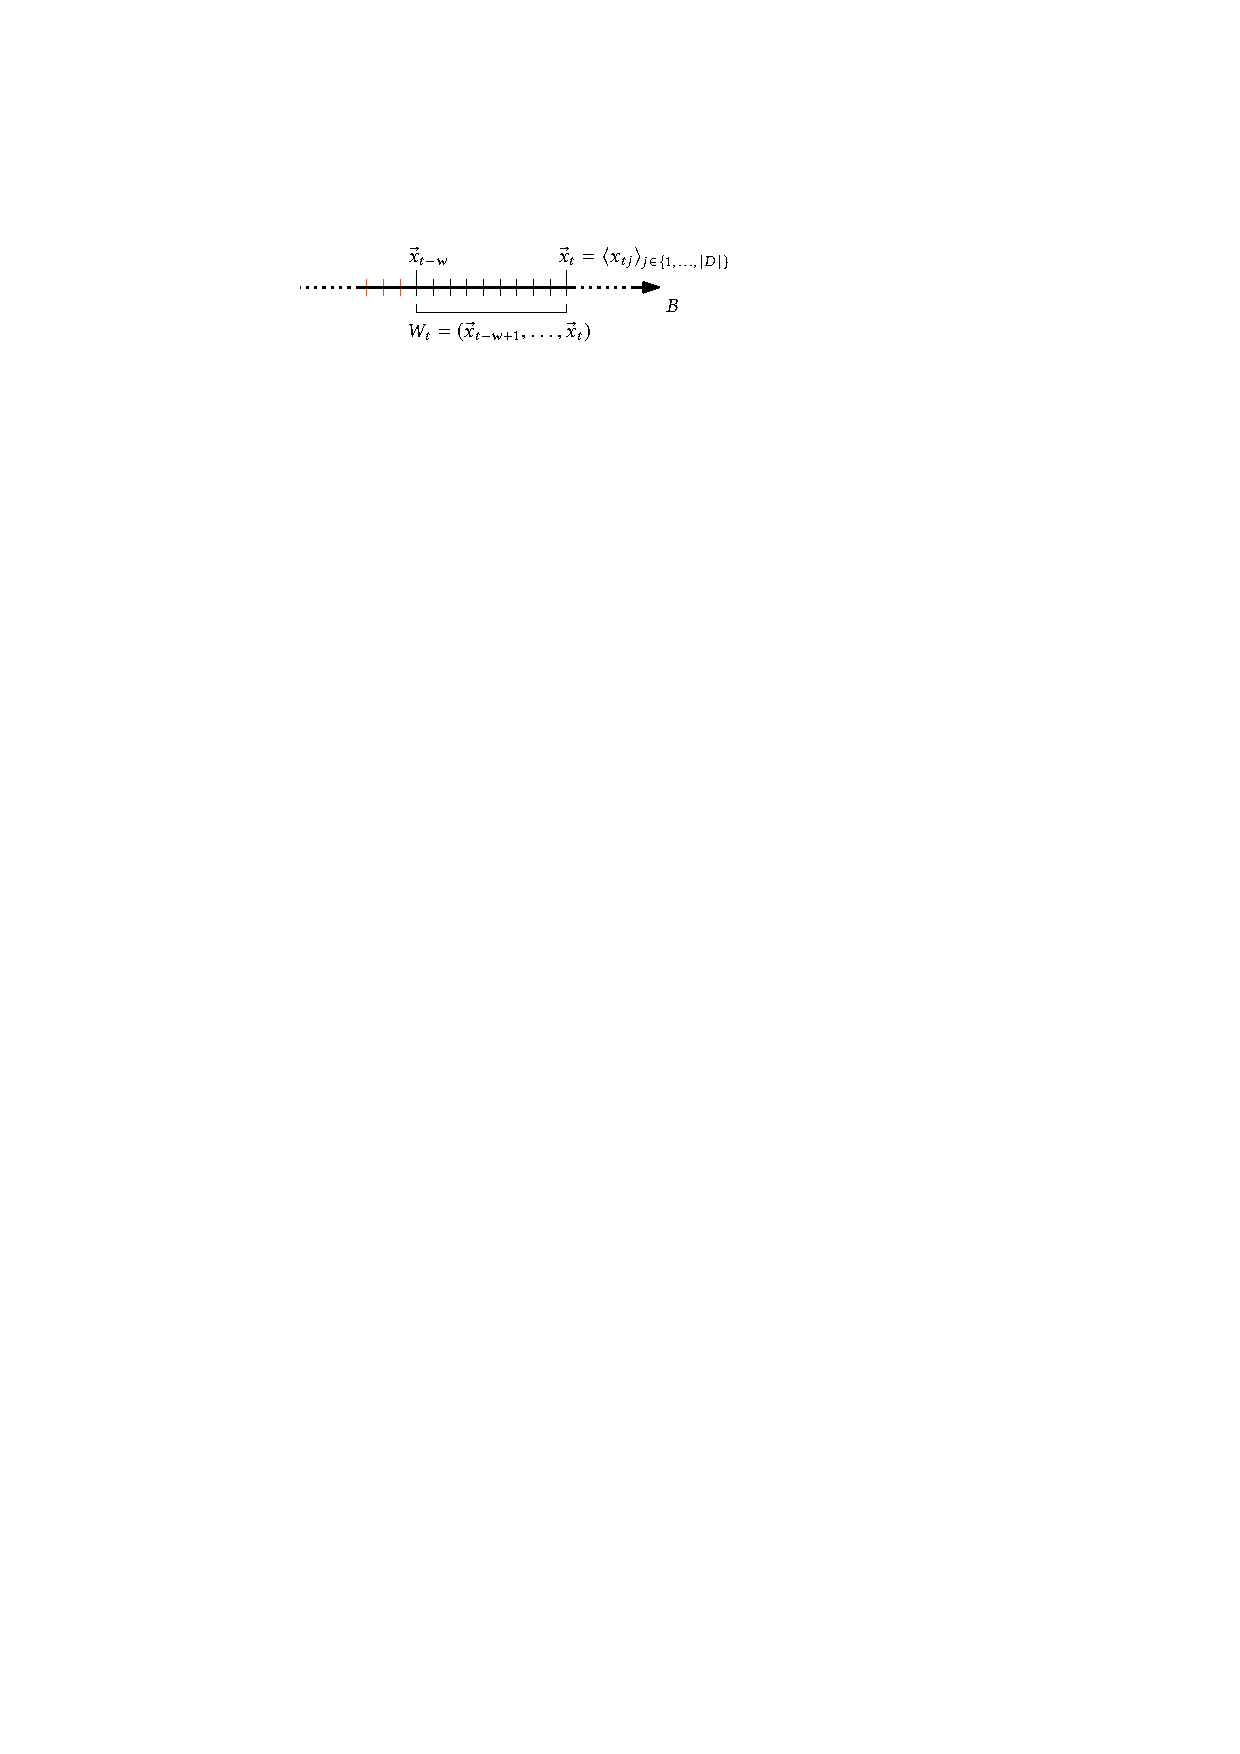
\includegraphics[width=0.6\textwidth]{part1-figures/slidingwindow-compressed.pdf}
	\caption{The sliding window contains the $\gls{w}$ latest observations (here, $\gls{w}=10$).}\label{fig:slidingwindow}
\end{figure}

We call a subspace $\gls{S}$ a projection of the window $\gls{W_t}$ on $|\gls{S}|$ attributes, with $\gls{S} \subseteq \gls{D}$ and $|\gls{S}| \leq |\gls{D}|$. 
We treat an attribute $\gls{s_i} \in \gls{D}$ as a random variable $\gls{X_{s_i}}$.  To address \textit{heterogeneity}, we also make the distinction between numerical, ordinal and categorical attributes:
\begin{itemize}[noitemsep]
	\item We say that $\gls{s_i}$ is of numerical type ($\gls{s_i} \in \mathit{\gls{Num}}$) 
	if one can see $\gls{X_{s_i}}$ as a continuous variable on a given interval. 
	\item We say that $\gls{s_i}$ is of ordinal type ($\gls{s_i} \in \mathit{\gls{Ord}}$) if one can see  $\gls{X_{s_i}}$ as a discrete variable, i.e., it can take a finite number of ordered values.
	\item We say that $\gls{s_i}$ is of categorical type ($\gls{s_i} \in \mathit{\gls{Cat}}$) if  one can see $\gls{X_{s_i}}$ as a categorical variable, with a fixed amount of nominal categories.
\end{itemize}

Naturally, knowing whether a given attribute is numerical, ordinal or categorical requires domain knowledge. Typically, ordinal attributes have many tying values, while values from a numerical attribute are unique, given enough precision. On the other hand, values from categorical attributes might not be numeric and do not have any meaningfully ordering. 

Then, $\gls{p(X)}$ is the joint probability distribution function (\textit{pdf}) of a random vector $\gls{X} = \left \langle \gls{X_{s_i}}\right \rangle  _{\gls{s_i} \in \gls{S}}$, and $\hat{p}(X)$ denotes the empirical estimation of this distribution. 
We use $\gls{p_{s_{i}}(X)}$ and $\hat{p}_{s_{i}}(X)$ for the marginal \textit{pdf} and its estimation for each variable $\gls{s_i}$.
$\gls{P}(\gls{S})$ is the power set of $\gls{S}$, i.e., the set of all attribute subsets. 
For any subset $S' \in \gls{P}(\gls{S})$, its random vector is $\gls{X}_{S'}= \left \langle \gls{X_{s_i}}\right \rangle _{\gls{s_i} \in S'}$ and its complement $\overline{X_{S'}} = X_{\gls{S}  \setminus S'} = \left \langle \gls{X_{s_i}}\right \rangle _{\gls{s_i} \in \gls{S} \setminus S'}$. 
In our algorithms, `$\oplus$' and `$\wedge$' stand for concatenation and element-wise logical conjunction. 

Dependency estimation determines to which extent a relationship differs from randomness. In this spirit, \gls{MCDE} quantifies a dependency, i.e., a degree of independence violation, based on marginal and conditional distributions. In Part \ref{partII}, we extensively describe \gls{MCDE}. 

Nonetheless, \gls{MCDE} only estimates the dependency within a given subspace. In the next section, we abstract from the underlying dependency estimator and consider the problem of monitoring numerous estimates in high-dimensional data streams. 

\section{Monitoring}

\subsection{Motivations} 
%Note: According to S. Muthukrishnan et al. Data streams: Algorithms and applications, I am using the time-series model (as opposed to additive and turnstile) (source: Boidol)

Monitoring, i.e., the real-time computation of statistics (such as dependency estimates), is crucial for Knowledge Discovery in data streams. Transient statistics may reveal the
current state of manufacturing machines or the ongoing behaviour of financial markets. 

However, monitoring is computationally demanding, especially when the number of dimensions and the rate of incoming data increase (cf. Sections \ref{challenges:highdimensionality} and \ref{challenges:datastreams}). %First, the number of pairs/subspaces grows quadratically/exponentially with the number of variables (cf. Section \ref{challenges:highdimensionality}). Second, a stream may evolve in unforeseen ways, i.e., each statistics become a time-dependent concept (cf. Section \ref{challenges:datastreams}). 
In this setting, recomputing the statistics at every time step does not scale. Thus, stream statistics monitoring -- for say, high-frequency trading or the monitoring of large factories -- is impractical with current methods. At the same time, it can be advantageous. Think for example of monitoring dependency in the \gls{Bioliq} plant: 

\begin{example}[Dependency Monitoring]
	\label{bandit:runningexample}
	Dependency often results from physical relationships between, say, the temperature and pressure of a fluid. 
%	When dependency changes, this means that the system is transitioning into another state, e.g., the fluid solidifies, or that equipment deteriorates or fails, e.g., there is a leak.
	When monitoring the pyrolysis process at \gls{Bioliq}, it is useful to maintain an overview of dependencies to keep operation costs down.  
	However, continuously updating the complete dependency matrix is impractical with current methods since the data is typically high-dimensional and ever-evolving. 
\end{example}

From a practical point of view, all statistics are not equally interesting. For example, for Knowledge Discovery, one is often interested in high dependency. Our idea is to update only a few elements of the matrix, based on a notion of `utility', e.g., high dependency values. The system must minimise the cost of monitoring while maximising the total utility. %, in a possibly non-static environment. 
In other words, the system faces a trade-off between exploitation and exploration: Should the system keep updating estimates known to deliver large utility (gain) or use resources to update other estimates, for which the potential utility is not yet well-known? 

%Put differently, one idea is to periodically update only a portion of the statistics over time, following a strategy that is learned online, i.e., the monitoring system decides which estimate to update. Based on the outcome, the system adjusts its strategy for future decisions. 

In this dissertation, we see the problem of monitoring as a generalisation of the \gls{MAB} problem. The \gls{MAB} problem captures the dilemma between exploration and exploitation in sequential decision-making. At every time step, a forecaster selects a set of arms and observes a reward from each arm. The name of the \gls{MAB} problem finds its origin in the typical trade-off a gambler faces in a casino: given a set of slot machines (see Figure \ref{fig:MAB}), a.k.a.\ `one-armed bandits', which machine should the gambler play to maximise their expected gains? Should they try different machines (exploration) or keep playing the machine that they believe to be the best so far (exploitation)?   

\begin{figure}
	\centering
	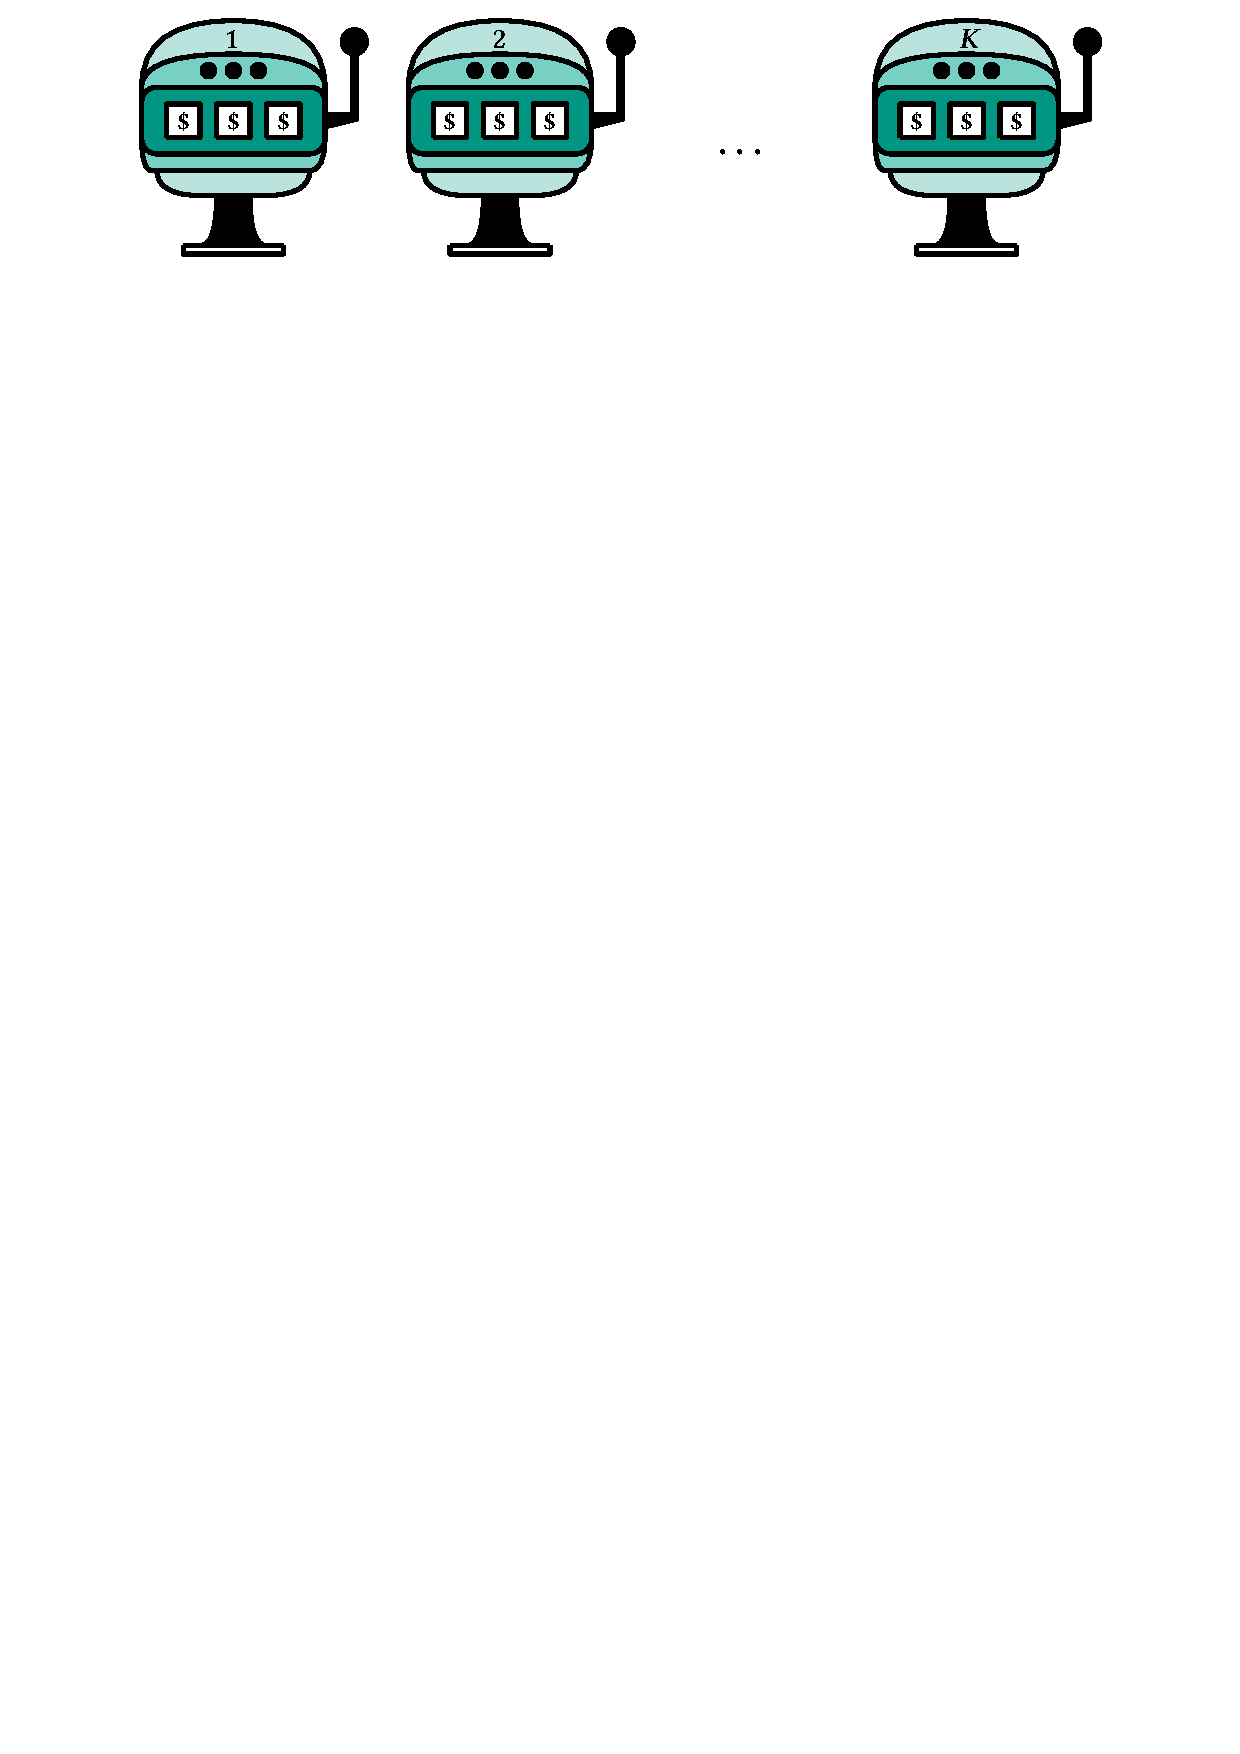
\includegraphics[width=0.70\textwidth]{part1-figures/bandit_1tok-compressed.pdf}
	\caption{The \acrshort{MAB} problem with $\gls{K}$ arms (one-armed bandits).}
	\label{fig:MAB}
\end{figure} 

However, the existing \gls{MAB} formulations do not quite match our problem, as we will see. In what follows, we propose to cast data stream monitoring as a new bandit problem, that we call the \gls{S-MAB}. 

\subsection{Monitoring as a Bandit Problem} 

In the classical \gls{MAB} problem, a forecaster must choose one of $\gls{K}$ arms at each round, and playing it yields a reward. Their goal is to maximise the cumulative reward over time. In a variant of the problem, known as the \gls{MP-MAB} \cite{1104491,DBLP:conf/icml/KomiyamaHN15}, the forecaster must choose $\gls{L}$ distinct arms per round, where $\gls{L}$ is an exogenous parameter. However, while it is relevant for some applications (e.g., web content optimisation), adequately setting $\gls{L}$ is not easy when monitoring streams. %, as well as further applications. %While in some applications, such as web content optimisation
%, $L$ is given, when monitoring data streams, an appropriate value of $L$ is not obvious. 

Thus, we consider a new variant of the \gls{MP-MAB} where the forecaster not only must choose the best arms but also must `scale' $\gls{L}$, i.e., change the number of plays, to maximise the rewards and minimise the costs. % at any time. 
By doing so, the forecaster controls the efficiency of playing. We name this setting the \acrfull{S-MAB} problem.

Think of a new casino game, which we call the `blind roulette': the player places bets on distinct numbers, and each number has an independent but unknown probability of being drawn. Bets correspond to a fixed amount, e.g., one can only bet $1$\$ on a number or nothing. 
In each round, the player must decide how many bets to place, and on which numbers. 
The casino then reveals to the player which ones of their bets were successful and pays the corresponding reward. To make the game more challenging, the casino may sometimes change the underlying probability of each number without notice.  

While placing a few but confident bets may seem to be an economically efficient option, the absolute gain at the end of the day will not be significant. 
On the other hand, placing many bets may not be a good strategy, as many numbers typically have a low chance to be drawn. 
To maximise their gain, the player must place as many bets as possible, as long as their expected gain is higher than the amount bet. 
Whenever the probabilities change, the player needs to adapt their behaviour; otherwise, they may lose most of their bets and experience much regret w.r.t.\ an optimal (but unknown) strategy.

This game matches not only dependency monitoring (cf. Example \ref{bandit:runningexample}) but also many other real-world applications, such as the placement of online advertisements or the investment in financial portfolios. The \gls{S-MAB} problem introduces a new trade-off: one wants to maximise the reward, but at the same time minimise the cost of each round/observation. The problem consists of the following challenges: 

\begin{itemize}[noitemsep]
	\item \hypertarget{*1}{\textbf{*1: Top-arms Identification.}} To maximise the reward from $\gls{L}$ plays, one needs to find the $\gls{L}$ arms with the highest expected reward; This is the traditional exploration-exploitation dilemma known from the \gls{MP-MAB} problem.
	
	\item \hypertarget{*2}{\textbf{*2: Scale Decision.}} One should not play more arms than necessary: playing many arms leads to high costs, but playing only a few arms leads to low rewards. One should set $\gls{L}$ to control the efficiency, i.e., the ratio of the rewards to the costs.
	
	\item \hypertarget{*3}{\textbf{*3: Change Adaptation.}} The environment can either be static or non-static. In the second case, one needs to `forget' prior knowledge whenever a change occurs. Forgetting that is too aggressive or too conservative leads to suboptimal results.
\end{itemize}
In the next section, we formalise the \gls{S-MAB} problem considering those challenges\footnote{See also \url{https://youtu.be/wVogcI3fr7Q} for a 3-minute introduction to this problem.}. We use the most common notation from the bandit literature, e.g., as in \cite{DBLP:journals/ftml/BubeckC12}. 

\subsection{Problem Definition}
\label{section:notationsbandits}

Let there be $\gls{K}$ arms. We associate each arm $i \in [\gls{K}]  = \left\{1,\dots,\gls{K}\right\}$ with an unknown probability distribution $v_i$ with mean $\gls{mu_i}$. 
At each round $\gls{t} = 1, \dots, \gls{T}$, the forecaster selects arms $\gls{I(t)} \subset [\gls{K}]$, then receives a reward vector $\gls{X(t)}$. 
$\gls{L}_{\gls{t}} \le \gls{K}$ is the number of these arms.
The rewards $\gls{X_i(t)} \in \gls{X(t)}$ of each arm $i$ are i.i.d.\ samples from $v_i$. We make the classical assumption from bandit analysis that the rewards $\gls{X_i(t)}$ are $0$ or $1$, i.e., the distribution of rewards from arm $i \in [\gls{K}]$ follows a Bernoulli distribution with mean $\gls{mu_i}$. 
Selecting an arm $i \in [\gls{K}]$ leads to a unit cost $1$, where cost and reward do not need to have the same unit. Note that it is not very difficult to generalise our results to other reward distributions, as long as they are bounded. 

Let $\gls{N_i(t)}$ and $\gls{S_i(t)}$ be the number of draws of arm $i$ and the sum of the rewards obtained from it respectively before round $t$. Let $\hat{\mu}_i(t) = \gls{S_i(t)}/\gls{N_i(t)}$ be the empirical estimation of $\gls{mu_i}$ at time $\gls{t}$. 
The forecaster is interested in maximising the sum of the rewards over arms drawn, under the constraint that the sum of the rewards must be greater than the sum of the costs by an efficiency factor $\gls{eta^*}$. The parameter $\gls{eta^*} \in [0,1]$ controls the trade-off between the cost of playing and the reward obtained, which is application-dependent. 

Let us think of our `blind roulette' metaphor and assume that, whenever a bet is successful, the casino awards the double of the bet. Then, for positive expectations, the player must set $\gls{eta^*} > 0.5$ and control $\eta_t$, the admitted cost per arm, to be higher than $\gls{eta^*}$. Thus, at each step $\gls{t}$, the forecaster is facing the following constrained optimisation problem: 
\begin{equation}
\underset{\gls{I(t)} \subset [\gls{K}]}{\max} \sum_{i \in \gls{I(t)}} \gls{S_i(t)} \quad s.t. \quad \eta_{\gls{t}} = \frac{\sum_{i \in \gls{I(t)}} \gls{mu_i}}{\gls{L}_{\gls{t}}}  > \gls{eta^*} 
\label{eq1}
\end{equation} 
The difficulty here is that the forecaster does not know $\gls{mu_i}$, but only has access to an estimate $\hat{\mu}_i$ from previous observations. 

$\sum_{i \in \gls{I(t)}} \gls{S_i(t)} $ is maximised when the forecaster chooses the arms with the highest expectation $\gls{mu_i}$. 
For simplicity, we assume that all arms have distinct expectations (i.e., $\gls{mu_i} \neq \mu_j, \forall i \neq j$) and we assume without loss of generality that $\mu_1 > \mu_2 > \dots > \mu_{\gls{K}}$, and thus $[\gls{L}_{\gls{t}}]$ is the top-$\gls{L}_{\gls{t}}$ arms. Under the assumption that the forecaster always chooses $[\gls{L}_{\gls{t}}]$, the value of $\eta_{\gls{t}}$ is only determined by $\gls{L}_{\gls{t}}$, i.e., Eq. \eqref{eq1} is equivalent to finding the optimal number of plays $\gls{L^*}$:
\begin{equation} \label{eq2}
\gls{L^*} = \underset{{1 \leq \gls{L} \leq \gls{K}}}{\max}{\gls{L}} \quad s.t. \quad \frac{\sum_{i=1}^{\gls{L}} \gls{mu_i}}{\gls{L}} > \gls{eta^*}
\end{equation}
Thus, the correct identification of the top-$\gls{L}_{\gls{t}}$ arms (\hyperlink{*1}{\textbf{*1}}) is sine qua non to find the optimal number of plays $\gls{L^*}$ (\hyperlink{*2}{\textbf{*2}}).
Next, in non-static environments, the expected rewards may change, i.e., $\gls{mu_i}: \gls{t} \mapsto [0,1]$ becomes a function of $\gls{t}$, as does $\gls{L^*}$. 
So the forecaster must adapt its estimation $\hat{\mu}_i$ (\hyperlink{*3}{\textbf{*2}}) to correctly select the arms with the highest reward, i.e., it needs to discard outdated observations. 

In Part \ref{partIII}, we present algorithms that solve the \gls{S-MAB} problem and those challenges. Using our contribution, one can monitor dependency in data streams very efficiently. In the next section, we start to reflect on the implications of those contributions w.r.t.\ Knowledge Discovery in high-dimensional data streams. 

\section{Knowledge Discovery}

Part \ref{partIV} shows the impact of our contributions towards a higher-level goal: Knowledge Discovery in high-dimensional data streams. Chapter \ref{chapter:subspacesearch} shows that combining our contributions from Part \ref{partII} and \ref{partIII}, namely \gls{MCDE} and \gls{S-MAB}, helps to transfer the task of subspace search to the streaming setting. We show that the efficient monitoring of subspaces of interest helps with outlier detection in high-dimensional data streams. Then, we deal in Chapter  \ref{chapter:textoutlier} with a real-world use case: the discovery of text outliers from large text corpora and propose a new method to detect such outliers. 

\subsection{Subspace Search in Data Streams}
\label{prelim:subspacesearch}

Analysing high-dimensional data is notoriously difficult (cf. Section \ref{challenges:highdimensionality}). As we discussed in Section \ref{sec:centralrole}, a fundamental task of Data Mining is to quantify the dependence between attributes. %This information helps to understand the data and often improves the result of subsequent Data Mining tasks. 
With this in mind, researchers have proposed \textit{subspace search} methods, mainly for static data, to find interesting low-dimensional projections. Such projections tend to much structure, i.e., high dependence among their dimensions. 
Subspace search is state-of-the-art to deal with data of high dimensionality and has numerous applications, including Exploratory Data Mining \cite{DBLP:journals/sigkdd/AssentKMS07, DBLP:conf/ieeevast/TatuMFBSSK12}, outlier detection \cite{DBLP:conf/icde/ZhangGW08, DBLP:conf/icde/KellerMB12,  DBLP:journals/ijdsa/TrittenbachB19}% vanea2012instant,
, or clustering \cite{DBLP:conf/sigmod/ProcopiucJAM02, DBLP:conf/pkdd/KailingKKW03, DBLP:conf/icdm/BaumgartnerPKKK04, DBLP:conf/cikm/ParkL07, DBLP:conf/icdm/ZhangLW07}.  %Some contributions \cite{DBLP:conf/aaai/WangRNBMX17, DBLP:conf/sdm/BohmKMNV13, DBLP:conf/cikm/KellerMWB13} explicitly address both clustering and outlier detection with the same subspace search approach. 

One can see subspace search as an ensemble \textit{feature selection} method \cite{DBLP:journals/jmlr/GuyonE03}, as the goal is to find several projections (subspaces), not just one. 
The underlying assumption of subspace search is that patterns (e.g., outliers, clusters) may hide in various subspaces \cite{DBLP:books/sp/Aggarwal2013}, and that, when restricting the search to a single subspace, one may miss some patterns. 
In a nutshell, existing subspace search methods consist of two building blocks: 

(1) A \textit{quality measure} to quantify the `interestingness' of a subspace, i.e., the potential to reveal patterns. Intuitively, subspaces with `structure' are more likely to contain outliers or clusters \cite{DBLP:phd/dnb/Keller15}. That measure often is a multivariate measure of dependence. 

(2) A \textit{search scheme} to explore the set of subspaces. Since this set grows exponentially with dimensionality, inspecting every subspace is not possible, and the search typically is a heuristic, i.e., a trade-off between completeness of the search and result quality.

These two items tend to be specific for a given Data Mining algorithm, e.g., a certain clustering method. 
The search then is helpful for this particular algorithm, but does not generalise beyond \cite{DBLP:conf/ieeevast/TatuMFBSSK12}. Next, existing approaches for subspace search tend to assume that the data is static. 
A straightforward generalisation to streams -- i.e., repeating the search periodically -- is computationally expensive and limited by the speed of new observations arriving. 

In Chapter \ref{chapter:subspacesearch}, we exploit synergies between our contributions \cite{DBLP:conf/ssdbm/FoucheB19, DBLP:conf/kdd/FoucheKB19, DBLP:conf/ssdbm/FoucheBMKB20} to facilitate subspace search in streams by fulfilling the constraints of this setting (see Section \ref{challenges:datastreams}). %Our algorithm, \gls{SGMRD}, facilitate subspace search for streams. 
The core idea of our method, \gls{SGMRD}, is to maintain a set of high-quality subspaces over time, by updating subspace-search results continuously. We show that it is advantageous to detect patterns (e.g., outliers) in high-dimensional data streams, and that existing approaches are much less efficient. To describe our approach, we use the same notation as in Section \ref{sec:mcdenotations}. 

%In the next section, we treat a more specific problem: The detection of outlying documents from large text corpora. 

\subsection{Mining Text Outliers}
\label{sec:textoutlierprelim}

\subsubsection{Motivations}

Recent technological developments have led to an ever-growing number of applications producing, sharing and managing text data. Document repositories, such as email accounts, digital libraries or medical archives, have grown so large that it is now a necessity to classify elements into categories, e.g., folders. 

This is far from trivial, as text corpora tend to be highly multi-modal, i.e., there are many classes/folders. 
Documents also may have ambiguous semantics or more than one semantic focus, so that they do not perfectly fit into just one class.
%EF: This introduces "Challenge 1: Multi-Modality"

Humans can order content to some extent and routinely do so: Users organise their emails into folders, authors classify their contributions into existing taxonomies, and physicians issue diagnoses as part of their duties. 
However, human classification is inherently sloppy and unreliable. %prone to errors. 
Humans may classify an email into an inadequate folder, assign scientific papers to the wrong field, or -- even more critical -- issue a wrong diagnosis. 
%EF: This introduces Type M (missclassification)

Sometimes one may not even notice these errors because the correct class is unknown. 
For instance, an email does not fit into any existing folder, a paper belongs to an emerging field, or a physician observes a new disease.  %EF: This introduces Type O (out-of-distribution)

\begin{figure}
	\centering
	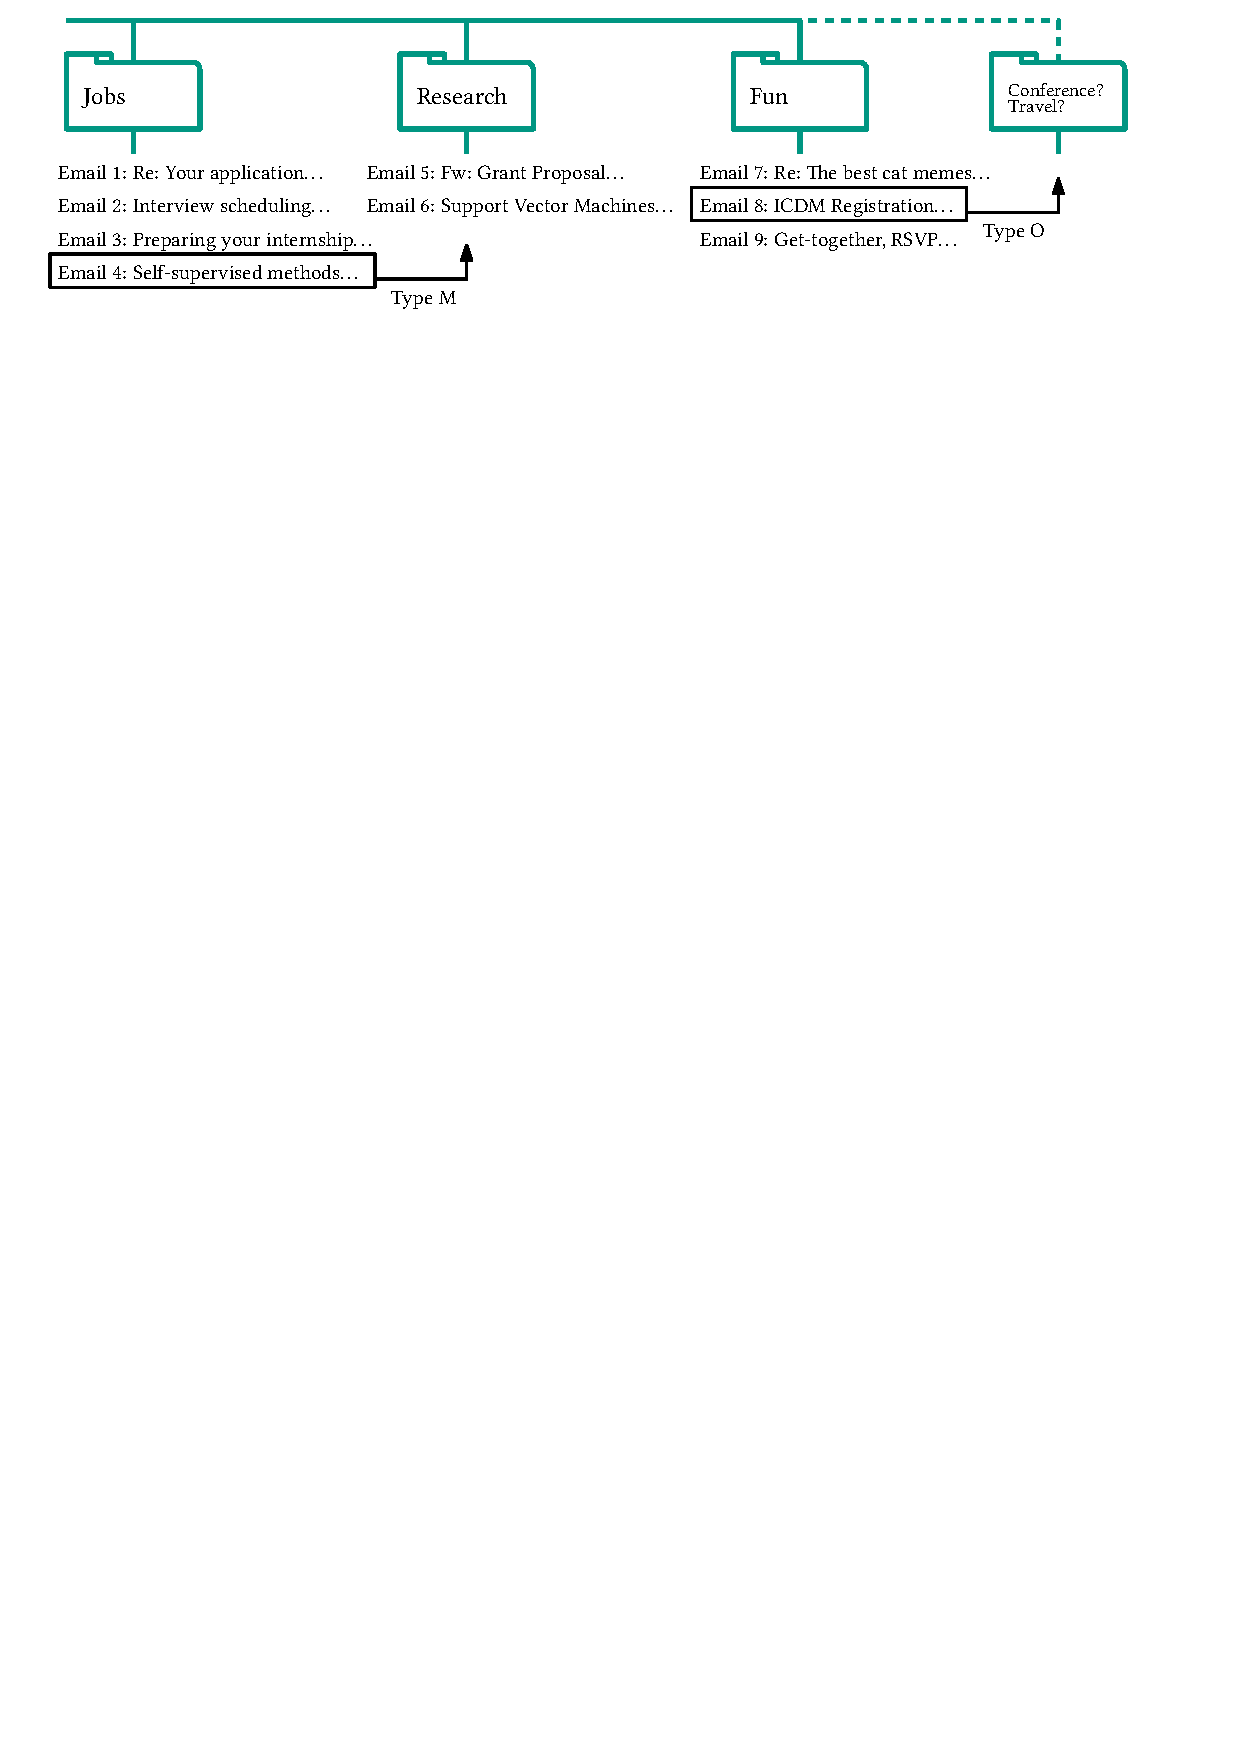
\includegraphics[width=\linewidth]{part1-figures/illustrative_example_2-compressed.pdf}
	\caption{Email Archiving: An Illustrative Example.}
	\label{fig:illustrative_example}
\end{figure}

Detecting documents classified erroneously is difficult \cite{DBLP:journals/tnn/FrenayV14, DBLP:series/isrl/2015-72}. This is because folder structures typically are domain-specific and are user-defined taxonomies. At the same time, documents can be misplaced in numerous, unforeseeable ways, which may or may not be folder-specific. 
So seeing this problem as a supervised one -- where a ground truth is available -- would be inadequate. Next, orthogonally to this `semantic' level, two types of errors/outliers can occur: \textbf{(O) Out-of-distribution}: A document does not belong to any existing folder --- the user should create a new class. % for Email 8.)
\textbf{(M) Misclassification}: A document belongs to another folder in the directory --- the user misclassified it.

We illustrate this in Figure~\ref{fig:illustrative_example}, with (fictitious) emails ordered into folders by a user: Email 4 is a Type~M outlier, as it belongs to the folder `Research'. Email 8 in turn is a Type~O outlier, because it does not fit into any existing folder --- we should create a new one. 
Intuitively, a document is a Type~O outlier when it does not appear to be similar to documents of any single class. 
In contrast, a document is a Type~M outlier when it appears to be most similar to documents from another class. 

In this work, we focus on mining text outliers in document directories. %Doing so improves existing text archives and supports the annotators. 
It is difficult  because documents are outlying w.r.t.\ their semantics, which is not easy to capture (even for humans). 
An additional issue, which makes this contribution unique, is that both outlier types must be detected jointly. 
Namely, the existence of one type harms the detection of the other one. 
The noise introduced by Type~M outliers hinders the detection of Type~O outliers. Conversely, Type~O outliers may be detected as Type~M by mistake, leading to a poor treatment of such outliers.
Existing methods only deal with one of these outlier types, cf.\ Section~\ref{relatedwork:MiningTextOutliers}. Interestingly, we show that the joint detection of both outlier types leads to better performance for each type than approaches only dealing with one of them. 
%This is suboptimal, as we will show.% in our study. 

To solve this problem, we propose a new approach to detect text outliers, which we name \gls{kj-NN}\footnote{See also \url{https://youtu.be/6dl3ZBxB3f0} for a 18-minute talk about our contribution.}. Our approach leverages similarities of documents and phrases, based on state-of-the-art embedding methods \cite{meng2019spherical}, to detect both Type~O/M outliers. By extracting semantically relevant labels and the documents similar to each outlier, it also supports interpretability. Our approach is efficient and robust to large proportions of erroneous labels thanks to a `self-supervision' mechanism, which estimates the relevance of the original labels. 
%Our idea is to weigh each decision by the relevance of neighbouring documents. A document is said to be relevant w.r.t.\ a given class when its semantics, characterised by its closest phrases in the embedding space, is representative of its class. 
Our experiments show that our approach improves the current state of the art by a large margin while delivering interpretable results. In the next section, we introduce our notation. 

\subsubsection{Notation}

Let $\gls{Doc} = \{\gls{d}_1, \gls{d}_2, \dots, \gls{d}_{|\gls{Doc}|}\}$ and $\gls{Phr} = \{\gls{p}_1, \gls{p}_2, \dots, \gls{p}_{|\gls{Phr}|}\}$ 
be a set of documents and phrases. We define $\gls{O} = \gls{Doc} \cup \gls{Phr}$ as the set of all text objects. 

A common practice in the community is to project each text object in an $n$-dimensional embedding space as a preprocessing step. In this paper, we use a recent technique \cite{meng2019spherical} capable of projecting both words and documents into the same embedding space, i.e., each object $\gls{o}$ has an embedding vector representation $\gls{V}: \gls{O} \mapsto \mathbb{R}^n$ with $n$ dimensions, with typically $n \geq 100$. The vectors are all normalised, thus $\| \gls{V}(\gls{o}) \| = 1,~\forall \gls{o} \in \gls{O}$.

We quantify the similarity between a pair of phrases, documents or phrases/documents with a function $\gls{Sim}: \gls{O}^2 \mapsto [0,1]$ where $1$ is the highest possible similarity (identity) and $0$ is the lowest one. In our setting, $\gls{Sim}$ is the normalised cosine similarity: 

\begin{equation}
\label{eq:cosinesimilarity}
\gls{Sim}(\gls{V}(\gls{o}_i), \gls{V}(\gls{o}_j)) = \frac{\gls{V}(\gls{o}_i) \cdot  \gls{V}(\gls{o}_j) + 1}{2} \quad \forall (\gls{o}_i, \gls{o}_j) \in \gls{O}^2
\end{equation}

For simplicity, we equivalently refer to the vectorial representation of each object, i.e., $\gls{o} \equiv \gls{V}(\gls{o})$, in what follows. We also assume that there exists an initial classification of documents into a set of classes $\gls{C} = \{\gls{c}_1, \dots, \gls{c}_{|\gls{C}|}\}$, expressed as a function $\mathit{\gls{y}}: \gls{Doc} \mapsto \gls{C}$. 

Our self-supervision mechanism relies on estimating the \textit{representativeness} of each phrase $\gls{p} \in \gls{Phr}$ w.r.t.\ each class $\gls{c} \in\gls{C}$. We denote it as a function $\mathit{\gls{r}}: \gls{Phr} \times \gls{C} \mapsto \mathbb{R}^+$. 

In Chapter \ref{chapter:textoutlier}, we extensively describe our approach and experiments. Note that for this study, we restricted our experiments to static text repositories. Nonetheless, our other contributions facilitate the extension of our approach to streams of text, e.g., news or twitter feeds. In that respect, one may see Chapter \ref{chapter:textoutlier} as preliminary work. Applying our methods for Knowledge Discovery in streams of text is future work (cf. Chapter \ref{chapter:futurework}). 


\chapter{Related Work}
\glsresetall
\label{chapter:relatedwork}

This chapter reviews the related work for each of our contributions.

\section{Estimating Dependency}

Estimating the dependency, or `correlation', between two or more variables, is a fundamental topic in data analysis and has motivated research for more than a century. Many bivariate measures exist, e.g., \cite{10.2307/1412159, 10.2307/1412159, 10.2307/2332226, Reshef1518}. Some of them also target at quantifying the association between two vectors which are possibly multivariate \cite{DBLP:conf/nips/GrettonFTSSS07, 10.2307/27801540, DBLP:conf/nips/Lopez-PazHS13, DBLP:conf/icml/BelghaziBROBHC18}. 
However, they can only quantify the dependency between two entities -- not between several ones (\hyperlink{R1}{\textbf{R1}}). %Note: this is known as canonical dependency estimation approaches 
They also may have other drawbacks. 
The Pearson correlation coefficient, for instance, is parametric  (\hyperlink{R4}{\textbf{R4}}), targets at linear dependencies (\hyperlink{R2}{\textbf{R2}}) and is only applicable to numerical data (\hyperlink{C5}{\textbf{C5}}).

There are attempts to extend bivariate dependency measures to the multivariate case. For example, there exists an extension of Spearman's $\rho$ to multidimensional data (\gls{MS}), but it is limited to monotonous relationships (\hyperlink{R2}{\textbf{R2}}). 
Several authors also propose multivariate extensions of \gls{MI} \cite{DBLP:journals/jcns/TimmeAFB14}. For example, \gls{II} \cite{DBLP:journals/tit/McGill54} quantifies the `synergy' or `redundancy' in a set of variables. Similarly, \gls{TC} \cite{DBLP:journals/ibmrd/Watanabe60} quantifies the total amount of information. 
However, information-theoretic measures are difficult to estimate, as they require knowledge about the underlying probability distributions. Density estimation methods, either based on kernels, histograms or local densities, 
all require setting unintuitive  parameters (\hyperlink{R3}{\textbf{R3}}) and may be computationally expensive (\hyperlink{C1}{\textbf{C1}}). Next, with many attributes, density estimation becomes meaningless due to the \textit{curse of dimensionality} \cite{bellman1957}. 
Information-theoretic measures also are difficult to interpret (\hyperlink{R5}{\textbf{R5}}), since they usually correspond to a number of bits or nats, which is theoretically unbounded. 

More recently, \gls{CMI},  \gls{MAC}, \gls{UDS},
\gls{UMC} and \gls{IID} were proposed as multivariate dependency measures. They are remotely related to concepts from information theory, as they rely on the so-called \gls{CE}. 
However, these measures are computationally expensive (\hyperlink{C1}{\textbf{C1}}) and unintuitive %to use
(\hyperlink{R3}{\textbf{R3}}). 
They also are difficult to interpret, because their theoretical maximum and minimum vary with the number of attributes (\hyperlink{R5}{\textbf{R5}}). 

Another approach, \gls{HiCS}, is somewhat similar to ours, \gls{MCDE}.
It uses \textit{subspace slicing} as a heuristic to quantify the potential of subspaces to contain outliers. Yet \gls{HiCS} only addresses static numerical data, and its suitability as a dependency estimator is not known. 

Also, most dependency estimators are designed to deal with numerical data only, and one assumes that all relevant observations are available during estimation. In the real world, however, data often consists of an open-ended, ever-evolving stream of measurements or indicators of various types, e.g., numerical, ordinal, or categorical observations.

The current state of the art to handle heterogeneity (\hyperlink{C5}{\textbf{C5}}) is to rely on discretisation, using methods such as the one proposed by \cite{DBLP:conf/ijcai/FayyadI93}. %,  as a pre-processing step. 
Then one can compute an information-theoretic measure, as in \cite{DBLP:conf/ssdbm/NguyenMAB14}. However, any discretisation essentially results in an information loss and may not work as dimensionality increases. %, because of data sparsity.

A recent line of work focuses on estimating \gls{MI} on numerical data streams. \gls{MISE} is a data summarisation technique to estimate \gls{MI} over arbitrary time windows. 
\cite{DBLP:conf/edbt/VollmerRB18} provide dynamic data structures to maintain \gls{MI} over a sliding window. % and provide lower bounds for the quality of estimates. 
\cite{DBLP:conf/edbt/VollmerB19} extend this method to propose an anytime estimator for \gls{MI}, with confidence bounds. 
However, the resulting estimates inherit the qualities and caveats from \gls{MI}. 

\section{Monitoring}

We refer to `monitoring' as the continuous surveillance of statistics in a multidimensional, potentially high-dimensional data stream. The existing approaches for monitoring statistics in streams fall into two classes: incremental and approximation schemes. 

\textbf{Incremental Schemes:} One can monitor statistics on  streams incrementally via a forgetting mechanism, to discard past observations. 
The approaches are usually based on a sliding window \cite{DBLP:conf/sdm/BifetG07, DBLP:conf/edbt/VollmerRB18} or a decaying factor \cite{koychev2000gradual, DBLP:journals/ida/Klinkenberg04, DBLP:conf/ssdbm/SchubertG18}. 
However, not every statistic can be computed incrementally, and the schemes only handle the computation of a single statistic, not of multiple ones. 

\textbf{Approximation Schemes:} Another line of research is approximating the statistics via sampling strategies \cite{DBLP:conf/soda/BabcockDM02, DBLP:conf/sac/BoidolH17, DBLP:conf/ssdbm/ArzamasovBR19} or data transformations, such as Fourier \cite{DBLP:conf/vldb/ZhuS02, DBLP:conf/iisa/SeliniotakiTCT14} or wavelet \cite{DBLP:journals/vldb/ChakrabartiGRS01, DBLP:conf/kdd/GuhaH05} transform. Other approaches explicitly target at high dependency \cite{DBLP:journals/ngc/KarguptaPKS06, DBLP:conf/kdd/ZhouX08}. However, most methods work only for specific statistics, e.g.,  Pearson's correlation, which limits their applicability to linear dependencies.  

Work on change detection also is related, as detecting whenever a change occurs in the stream helps with monitoring. \cite{DBLP:conf/sdm/NguyenV16a}, \cite{DBLP:conf/kdd/ReisFMB16} or \cite{DBLP:journals/tkde/BlancoCRBDM15} all aim to detect sudden changes. However, these approaches do not apply to stream data or require labels, which make them unsuitable for the high-dimensional streaming setting in general and further applications, e.g., predictive maintenance. % In Section \ref{bandits}, we give more details about how we intend to approach this problem. 

Our approach, \gls{S-MAB}, does not fall into these categories, since we target at monitoring virtually any statistics; the estimates are exact, but our algorithm decides when to update them. To do that, we show that our method can also leverage change detectors, such as \gls{ADWIN}. Thus, our contribution is orthogonal to the existing work. For a broader overview of stream monitoring methods, see \cite{DBLP:books/daglib/0030859}.

Since our approach bases on bandit theory, the existing bandit models also are related. Work on bandits traces back to \cite{Thompson1933}, with the design of clinical trials. %In 1953, behavioural psychologists \cite{Bush1953} coined the term \textit{bandit} in analogy to the well-known slot machines. 
The theoretical guarantees of bandits remained unknown until recently \cite{DBLP:journals/eccc/ECCC-TR00-068,DBLP:journals/ml/AuerCF02,Garivier2008, DBLP:conf/alt/KaufmannKM12}. Our work builds on several facets of bandits, which have been studied separately, such as anytime bandits \cite{DBLP:conf/soda/Kleinberg06, DBLP:conf/icml/DegenneP16}%slivkins2008adapting,garivier2018kl
, \gls{MP-MAB} \cite{1104491,DBLP:conf/alt/UchiyaNK10, DBLP:conf/icml/KomiyamaHN15} %agrawal1990multi 
and bandits in non-static environments \cite{DBLP:journals/siamcomp/AuerCFS02, DBLP:conf/colt/SlivkinsU08, DBLP:conf/alt/GarivierM11}. %However, to the best our knowledge, we are the first to consider all of these "complications" together. 

One can see the \gls{S-MAB} as an extension of the \gls{MP-MAB}, with the novelty that the player must control the number of plays over time. 
In particular, we build on the work from \cite{DBLP:conf/icml/KomiyamaHN15}.
It shows that \gls{MP-TS} has optimal regret while being efficient. We compare our results with other multiple-play models, such as variants of the celebrated \gls{UCB} and the \gls{Exp3}, namely \gls{CUCB}, \gls{MP-KL-UCB} and \gls{Exp3.M}. 

Our problem is different from the profitable bandits \cite{DBLP:conf/acml/AchabCG18} since they aim at maximising a static notion of profit -- as opposed to efficiency -- which boils down to finding the individual arms for which the rewards exceed the costs in expectation. 
Moreover, our problem is more challenging than the \gls{MP-MAB} and its extension called \gls{CMAB} in that we are interested in a set of arms where the model parameters $\mu_i$ satisfy an efficiency constraint (see Eq. \eqref{eq1}), and the algorithm needs to estimate them.

\glsunset{MAB}
The \gls{S-MAB} also is related to the budgeted \gls{MAB} model \cite{DBLP:conf/aaai/LongCCRJ10, DBLP:conf/ijcai/XiaQMYL16}%xia2015thompson
, because it aims at maximising a notion of efficiency, i.e., the ratio of the reward to the cost of playing arms.
In our case, the total number of plays -- the `budget' -- is not an external constraint. Instead, the \gls{S-MAB} decides how many arms to play based on its observations of the environment. %We also make the assumption that each arm is associated to the same cost. 

%Our approach also is related to \textit{combinatorial bandit} \cite{cesa2012combinatorial, chen2013combinatorial} and \textit{thresholding bandits} (link to clarify). % also restless bandits (Improving Online Marketing Experiments with Drifting Multi-armed Bandits)
%EF: Since our approach is "two-step", I find it a bit similar to Adapt-Eve too (which does not have any theoretical analysis, even if very good in practice)
%EF: The approach also shares similarities with Viappiani, Paolo. "Thompson sampling for bayesian bandits with resets." International Conference on Algorithmic DecisionTheory. (at difference of scaling and being multiple play, using ADWIN and not a particle filter)
% Also the multiple-play aspects is close to the "Non-Stochastic Bandit Slate Problems" (kale). 
%See also "A Change-Detection based Framework for Non-stationary Multi-Armed Bandit Problem") (UCB + Change point detection)
% Also,  SAO: Stochastic and Adversarial Optimal (Combines UCB1 and Exp3)
% "Surveillance in an Abruptly Changing World via Multiarmed Bandits" is somewhat related to the scaling bandit

% "On Upper-Confidence Bound Policies for Switching Bandit Problems" (Garivier11) is an archetypal example that considered abrupt changes, while "Slivkins, A., Upfal, E.: Adapting to a changing environment: the brownian restless bandits" considers distribution  of rewards that changes continuously
% According to "Hartland, C., Gelly, S., Baskiotis, N., Teytaud, O., Sebag, M.: Multi-armed bandit, dynamic environments and meta-bandits (2006)" standard soft-max and UCB policies are not appropriate for abruptly changing environments
% Some work on correlation monitoring: 
% COREQ: https://hpi.de/mueller/coreq.html
% FMC: "Minefleet: The vehicle data stream mining system for ubiquitous environments"
% Statstream: "Statstream: Statistical monitoring of thousands of data streams in real time"
% PeakSim: "Stream correlation monitoring for uncertainty-aware data processing systems"

Bandits have readily been applied to many real-world applications, such as packet routing \cite{DBLP:conf/stoc/AwerbuchK04}, online advertising \cite{DBLP:conf/nips/ChakrabartiKRU08}, recommendation systems \cite{DBLP:conf/www/LiCLS10}, robotic planning \cite{DBLP:conf/cdc/SrivastavaRL14} and resource allocation \cite{DBLP:journals/pvldb/LiZLWZ18}. 
Nonetheless, the application of bandits to monitoring (see Example \ref{bandit:runningexample}) has received much less attention.
For an overview of bandit algorithms, we refer the reader to recent surveys \cite{DBLP:journals/ftml/BubeckC12, DBLP:journals/corr/BurtiniLL15, lattimore18}.   

%\begin{itemize}
%	\item Useful fundamentals and formalisms: \cite{Bubeck2012}
%	\item Useful survey: \cite{burtini2015survey}
%	\item Non-static: Discounted UCB / Sliding Window UCB \cite{Garivier2008}, surveillance (switching window) \cite{srivastava2014surveillance}
%	\item Contextual Bandits: survey \cite{zhou2015survey}, efficient optimal learning \cite{dudik2011efficient}, mobile health \cite{tewari2017ads}
%	\item Adversarial and multiple play: \cite{uchiya2010algorithms}
%	\item Multiple play: ad placement \cite{louedec2015multiple}, thompson sampling \cite{komiyama2015optimal}, budgeted \cite{xia2016budgeted}
%	\item Budgeted: budget-limited (Ph.D. thesis) \cite{tran2012budget}, finite budget analysis \cite{xia2017finite}, many-arm \cite{li2017infinitely}, thompson sampling \cite{xia2015thompson}
%	\item Adversarial: adaptive algorithms \cite{wei2018more}, Exp3++ \cite{seldin2017improved}, Boltzmann exploration \cite{cesa2017boltzmann}
%	\item Anytime: \cite{besson2018doubling}, online portfolio choice \cite{shen2015portfolio}
%	\item Non-static: \cite{allesiardo2017non}, restless (website optimization) \cite{burtini2015improving}, restless (seminal paper) \cite{whittle1988restless} 
%	\item Following-the-perturbed-leader: \cite{hutter2005adaptive}
%\end{itemize}

\section{Knowledge Discovery}

% Maybe relevant: Sliding window-based fault detection from high-dimensional data streams L Zhang, J Lin, R Karim
% Maybe relevant: An angle-based subspace anomaly detection approach to high-dimensional data: With an application to industrial fault detection L Zhang, J Lin, R Karim
% Maybe relevant: An adaptive algorithm for anomaly and novelty detection in evolving data streams Mohamed-Rafik Bouguelia, Slawomir Nowaczyk & Amir H. Payberah 
% Maybe also: Deep Incremental Learning for Big Data Stream Analytics SA Alex, JJV Nayahi 
% Maybe also: An improvement growing neural gas method for online anomaly detection of aerospace payloads L Song, T Zheng, J Wang, L Guo

Because of the unsupervised nature of tasks in high-dimensional streams, knowledge discovery mainly is limited to two classes of applications: outlier/anomaly detection and clustering. As mentioned in recent studies \cite{DBLP:conf/ssdbm/KriegelKNZ11,DBLP:conf/sdm/NtoutsiZPKK12}, little effort was devoted so far to the discovery of patterns in high-dimensional data streams. Most contributions focus instead on only one of the two aspects: high-dimensionality or data streams. 

While recent studies, such as \cite{DBLP:conf/vldb/AggarwalHWY04, DBLP:conf/icde/ZhangGW08, DBLP:conf/ssdbm/KriegelKNZ11, DBLP:conf/sdm/NtoutsiZPKK12}, attempt to address high-dimensional data streams, the dimensionality in benchmarks is limited -- usually, to less than $50$ dimensions. Thus, whether those approaches can scale is not known. Recent surveys \cite{DBLP:journals/tkde/GuptaGAH14, DBLP:journals/jcst/AminiTS14} provide a good overview of the state-of-the-art methods for Knowledge Discovery in data streams w.r.t. the task of outlier detection and clustering.

While addressing every Knowledge Discovery problem is out of the scope of this dissertation, the fundamental nature of our contributions helps towards this goal. We focus in particular on two Knowledge Discovery tasks: `Subspace Search in Data Streams' and `Mining Text Outliers', for which we detail the related work hereafter. 

\subsection{Subspace Search in Data Streams}

Many methods for subspace search exist, but almost all of them are either coupled to a specific Data Mining algorithm or are limited to the static setting. 
For example, various approaches for streams \cite{DBLP:conf/ideas/KontakiPM06, DBLP:conf/icdm/ZhangLW07, DBLP:conf/icde/ZhangGW08, DBLP:conf/icde/Aggarwal09a} % vanea2012instant
only tend to work with a given static algorithm. Other methods in turn \cite{DBLP:conf/icde/KellerMB12, DBLP:conf/sdm/BohmKMNV13, DBLP:conf/bigdataconf/NguyenMB13, DBLP:conf/sdm/NguyenMV16, DBLP:conf/aaai/WangRNBMX17, DBLP:journals/ijdsa/TrittenbachB19} decouple the search from the actual task, but none of them can handle streams. The existing work on subspace search mostly focuses on individual applications \cite{DBLP:journals/sigkdd/ParsonsHL04, DBLP:journals/tkdd/KriegelKZ09, DBLP:journals/sadm/ZimekSK12}, e.g., clustering or outlier detection, while `general-purpose' subspace search has received less attention. 

To our knowledge, there exist two proposals to extend subspace search to streams in a general way: HCP-StreamMiner \cite{vanea2012instant} and Stream\gls{HiCS} \cite{becker2016concept}. 
But these approaches boil down to a periodic repetition of the procedure in \cite{DBLP:conf/icde/KellerMB12} on synopses of the stream. 
We will see that our method outperforms these approaches. %, while requiring much less computation. 
\gls{GMD} is the approach most similar to ours. 
It uses a so-called contrast measure \cite{DBLP:conf/icde/KellerMB12} to quantify the interestingness of a given subspace and builds a set of subspaces via a greedy heuristic. 
However, \gls{GMD} assumes static data.

Subspace search has been used in the past to improve the results of Data Mining tasks such as outlier detection \cite{DBLP:conf/icde/ZhangGW08, DBLP:conf/icde/KellerMB12,  DBLP:journals/ijdsa/TrittenbachB19}. The authors compare their results with full-space static outlier detectors. %There exists a plethora of methods for outlier detection, both in the static and streaming setting. 
We perform an analogous evaluation in the streaming setting and compare our results against several baselines and state-of-the-art stream outlier detectors, such as xStream \cite{10.1145/3219819.3220107} and \gls{RS-Stream}. See \cite{DBLP:journals/tkde/GuptaGAH14} for a survey of outlier detection in streams.

\subsection{Mining Text Outliers}
\label{relatedwork:MiningTextOutliers}
%In this section, we review existing studies for document-level outlier detection. 
\glsunset{kj-NN}

To our knowledge, none of the existing methods handles both outlier types. 
So we categorise related work into two classes: (1) Type~O and (2) Type~M outlier detectors. 

\textbf{Type~O outlier detectors.} Type~O is the standard definition of outliers, and detecting such outliers has been studied for decades. 
Conventional outlier detection approaches typically fall into the following classes: distance-based \cite{knox1998algorithms,ramaswamy2000efficient}, neighbour-based \cite{DBLP:conf/sigmod/BreunigKNS00,kriegel2008angle}, probabilistic-based \cite{kim2012RKDE,tipping1999PPCA} and subspace-based methods \cite{DBLP:journals/kais/SatheA18,lazarevic2005feature,muller2012outlier,DBLP:conf/icde/KellerMB12,kriegel2012outlier}. Examples of conventional methods are the well-known \gls{LOF} or, more recently, \gls{RS-Hash}. However, textual data is typically extremely sparse, and thus few of the above proposals can detect outlier documents, as they do not model semantics.

There exist a few methods addressing text outliers: \cite{DBLP:conf/emnlp/ZhuangWTKH17} proposes a generative approach, which models the embedding space as a mixture of von \gls{vMF} distributions. They identify `outlier regions' that deviate from the majority of the embedded data. \acrshort{TONMF} \cite{DBLP:conf/sdm/KannanWAP17}, a Non-negative Matrix Factorisation (NMF) approach, bases on block coordinate descent optimisation. 
Recently, Ruff et al.\ proposed \gls{CVDD}, a one-class classification model leveraging pre-trained language models and a multi-head attention mechanism. However, all of these methods treat outlier detection as a one-class classification problem, i.e., they try to describe an `abnormal' class and a `normal' class; none of them addresses Type~M outliers. 

\textbf{Type~M outlier detectors.} Type~M outliers represent misclassified text. While this type of outlier is ubiquitous, it has received little attention so far. 
Few publications try to address the problem directly. 
Traditional supervised text classification methods, assuming the ground truth to be error-free, have no choice but to tolerate Type~M outliers during training. 
While one can extend the existing supervised document classification models (e.g., \cite{DBLP:conf/emnlp/Kim14, DBLP:conf/eacl/SchwenkBCL17, DBLP:conf/acl/ZhouSTQLHX16, DBLP:conf/aaai/LaiXLZ15}) to mitigate the effect of Type~M outliers, they are in turn not helpful to detect Type~O outliers. 

As we explained earlier, the existence of both outlier types calls for methods that can detect them simultaneously. In that respect, our method, \gls{kj-NN}, is the first of its kind. In our experiments, we compare our approach against the methods above and show that we outperform all of them. We refer the reader to \cite{DBLP:books/sp/Aggarwal2013} for an extensive overview of existing outlier detection methods. 

%Some further elements: 
%Novelty detection \cite{zhang2005probabilistic, zhang2002novelty, kasiviswanathan2012online, kasiviswanathan2013novel} [Handling type A only]. 
%\cite{DBLP:journals/sigkdd/SunH12} identifies our focus as an important challenge. 
%Document clustering, classification [...]. Clustering is often useful for Type A outliers, while classification for Type B. 
%WeSTClass \cite{DBLP:conf/cikm/MengSZ018}, WeSHClass \cite{DBLP:conf/aaai/MengSZH19} targets at text classification with weak supervision [No outlier detection, i.e., no Type A, different setup]. 
%Zero-shot classification \cite{DBLP:conf/naacl/ZhangLG19} [?]. 
%\cite{barigou2016improving} is related work, it uses k-NN for text classification (TODO: clarify the relationship). 
%Maybe rule out the effort made in the crowdsourcing community as we may not use any kind of majority voting (no consensus possible). 
%Maybe discuss that kNN can be used as an outlier detection method, but quite in a different way (usually extensions like LOF \cite{DBLP:journals/datamine/CamposZSCMSAH16}). 
%Topic modelling [?]. 
%Graph outlier ranking method \texttt{GOutRank} \cite{DBLP:conf/icde/MullerSMB13}. 
%Community distribution outlier detection CDODA \cite{DBLP:conf/pkdd/GuptaGH13}. 
%Embedding methods: JoSE \cite{meng2019spherical} on which we are building, probably need to consider Doc2Vec \cite{DBLP:conf/icml/LeM14} also. 
%\item \texttt{RankClus} \cite{DBLP:conf/edbt/SunHZYCW09}, historical word on heteregeneous information networks (bi-typed), as well as its follow-up \texttt{NetClus} \cite{DBLP:conf/kdd/SunYH09} (star-schema)
%\item \texttt{KnowSim} \cite{DBLP:conf/icdm/WangSLZH15} similarity measure on HIN
% See \url{https://github.com/brightmart/text_classification} for some type B baselines.

\part{Estimating Dependency}
\label{partII}

\chapter{\acrlong{MCDE}}
\glsresetall
\label{chapter:MCDE}

The content of this chapter bases on the following publications: 

\begin{itemize}[noitemsep]
	\item \fullcite{DBLP:conf/ssdbm/FoucheB19}
	\item \fullcite{DBLP:conf/ssdbm/FoucheBMKB20}
\end{itemize}
\textbf{Keywords:} Multivariate Statistics; Exploratory Data Analysis; Dependency Estimation % Data Mining;  

\section{Chapter Overview} 

Estimating dependencies from data is a fundamental task of Knowledge Discovery. Identifying the relevant variables leads to a better understanding of data and improves both the runtime and the outcomes of downstream Data Mining tasks. 
Dependency estimation from static numerical data has received much attention.
However, real-world data often occurs as heterogeneous data streams. In this chapter, we make the following contributions:

\textbf{We present \gls{MCDE}}, a framework which satisfies both the constraints of heterogeneous data streams and the requirements of dependency estimation. Over a given time window, \gls{MCDE} estimates the dependency of an attribute set as the average discrepancy between marginal and conditional distributions, via Monte Carlo (MC) simulations. %In each MC simulation, MCDE applies a condition on each attribute. Then a statistical test quantifies the discrepancy between the marginal and conditional distributions. 
We determine a lower bound for the quality of our estimates, which only depends on the number of MC simulations. Such bound allows users to trade estimation accuracy for a computational advantage. 

\textbf{We explore three instantiations of \gls{MCDE}}, i.e., three new dependency measures, dubbed \gls{MWP}, \gls{KSP} and \gls{CSP}, which base on the corresponding statistical test. We show that using them in combination allows dealing with heterogeneous data. 
We describe their implementation and compare them to the existing multivariate methods in our experiments. 

\textbf{We introduce index structures} for \gls{MWP}, \gls{KSP}, and \gls{CSP}, to speed up contrast estimation. Our indexes support insertion/deletion operations for efficient estimation in streaming settings, e.g., over a sliding window.

\glsunset{Bioliq}
\textbf{We feature a use case against real-world data} from \gls{Bioliq} (cf. Section \ref{sec:bioliqexample}) and show how one can leverage \gls{MCDE} to discover interesting and useful patterns. We release our source code and experiments on GitHub\footnote{\url{https://github.com/edouardfouche/MCDE-experiments}}\textsuperscript{,}\footnote{\url{https://github.com/edouardfouche/MCDE-extended}}, with documentation to ensure reproducibility.

\section{Theory of \acrshort{MCDE}}

Dependency estimation determines to which extent a relationship differs from randomness. In this spirit, \gls{MCDE} quantifies dependence, i.e., a degree of independence violation, based on marginal and conditional distributions. Section \ref{sec:mcdenotations} introduced our notation. 

\subsection{Quantifying Dependency via Contrast}

A set of variables is \textit{independent} or \textit{uncorrelated} if and only if all variables are pairwise \textbf{mutually independent}. 
By treating the attributes of a subspace as random variables, we can define the independence assumption of a subspace: 
\begin{definition}[Independence Assumption]
	\label{IA1}
	The independence assumption $\mathcal{A}$ of a subspace $\gls{S}$  holds if and only if the random variables $\{ \gls{X_{s_i}} : \gls{s_i} \in \gls{S} \}$ are mutually independent, i.e.:
	\begin{equation}
	\mathcal{A}(\gls{S}) \Leftrightarrow \gls{p(X)} = \prod_{\gls{s_i} \in \gls{S}} \gls{p_{s_{i}}(X)} \label{eq:IA1}
	\end{equation}
\end{definition}
Under the independence assumption, the joint distribution of subspace $\gls{S}$ is \textbf{expected} to be equal to the product of its marginal distributions. We can define a degree of dependency %, or correlation, 
based on the degree to which $\mathcal{A}$ does not hold: 
\begin{definition}[Degree of Dependency]
	\label{DependencyDegree}
	The degree of dependency $\mathcal{D}$ of a subspace $\gls{S}$ is the discrepancy, abbreviated as `$disc$', between the \textbf{observed} joint distribution $p^{o}(\gls{X})$ and the \textbf{expected} joint distribution $p^{e}(\gls{X})$: 
	\begin{equation}
	\mathcal{D}(\gls{S}) \equiv disc \left(p^{o}(\gls{X}),p^{e}(\gls{X})\right) 
	\end{equation}
\end{definition} 
The discrepancy is a random variable. 
While one can estimate it between two probability distributions, using for instance the Kullback-Leibler divergence, %\cite{kullback1951information}
 this is not trivial here because $p^o(\gls{X})$ and $p^{e}(\gls{X})$ are a priori unknown. We work around this as follows: 
\begin{lemma}[Independence Assumption and Joint Distribution]
	\label{lemma1}
	The independence assumption $\mathcal{A}$ of subspace $\gls{S}$ states that the joint distribution for all  $S' \subset \gls{S}$  is equal to its conditional distribution on $\gls{S} \setminus S'$:
	\begin{equation}
	\mathcal{A}(\gls{S}) \Leftrightarrow p(X_{S'}|\overline{X_{S'}}) =  p(X_{S'}) \quad \forall S' \in \gls{P}(\gls{S})
	\end{equation}
\end{lemma} 
\begin{proof}[Proof of Lemma \ref{lemma1}]
	Since all variables in $\gls{S}$ are mutually independent, for any subspace $S' \in \gls{P}(\gls{S})$ we also have $p(X_{S'}) = \prod_{\gls{s_i} \in S'} \gls{p_{s_{i}}(X)}$:
	\begin{align*}
	\mathcal{A}(\gls{S}) &\Leftrightarrow~ \gls{p(X)} = \prod_{\gls{s_i} \in \gls{S}} \gls{p_{s_{i}}(X)} &&~ \\
	\mathcal{A}(S) &\Leftrightarrow~ \gls{p(X)} = p(X_{S'}) * \prod_{\gls{s_i} \in \gls{S} \setminus S'} \gls{p_{s_{i}}(X)} && \forall S' \in \gls{P}(\gls{S}) \\
	\mathcal{A}(\gls{S}) &\Leftrightarrow~ \frac{\gls{p(X)}}{p(\overline{X_{S'}})} = p(X_{S'}) && \forall S' \in \gls{P}(\gls{S})
	\intertext{By the definition of the conditional \textit{pdf}:}
	\mathcal{A}(\gls{S}) &\Leftrightarrow~ p(X_{S'}|\overline{X_{S'}}) =  p(X_{S'}) && \forall S' \in \gls{P}(\gls{S}) \label{lastofproof1} 
	\qedhere
	\end{align*}
\end{proof}

Lemma \ref{lemma1} provides an alternative definition of $\mathcal{A}$. However, it still has issues. % for the following reasons: 
First, multivariate density estimation is required to estimate $p(X_{S'})$ and $p(X_{S'}|\overline{X_{S'}})$ with $|S'| \geq 1$. 
Second, even if one could estimate $p(X_{S'})$ and $p(X_{S'}|\overline{X_{S'}})$, estimating the densities for all $ S' \in \gls{P}(\gls{S})$ is intractable. 
We instead relax the problem by considering only subspaces with  $|S'| = 1$, i.e., we only look at the marginal distribution of single variables. 
\begin{definition}[Relaxed Independence Assumption]
	The relaxed independence assumption $\mathcal{A}^*$ of a subspace $\gls{S}$ states that 
	the marginal distribution $\gls{p_{s_{i}}(X)}$ of each variable $\gls{s_i} \in \gls{S}$ equals $p_{s_{i}}(X|\overline{X_{s_i}})$, i.e., the conditional distribution of $\gls{s_i}$:
	\begin{align*}
	\mathcal{A}^*(\gls{S}) \Leftrightarrow p_{s_{i}}(\gls{X}|\overline{X_{s_i}}) = \gls{p_{s_{i}}(X)} \quad \forall \gls{s_i} \in \gls{S} 
	\end{align*}
\end{definition}

\begin{lemma}[Independence Assumption Relaxation] 
	\label{IA2}
	$\mathcal{A}(\gls{S}) \Rightarrow \mathcal{A}^*(\gls{S})$, i.e., we can relax $\mathcal{A}$ into $\mathcal{A}^*$ for any subspace $\gls{S}$.
\end{lemma}
\begin{proof}[Proof of Lemma \ref{IA2}]
	Using Lemma \ref{lemma1}:
	\begin{align*}
	\mathcal{A}(\gls{S}) &\Leftrightarrow p(X_{S'}|\overline{X_{S'}}) =  p(X_{S'}) && \forall S' \in \gls{P}(\gls{S}) \\
	\mathcal{A}(\gls{S}) &\Rightarrow p(X_{S^1}|\overline{X_{S^1}}) = p(X_{S^1}) && \forall S^1 \in \gls{P}(\gls{S}) :|S^1| = 1\\
	\mathcal{A}(\gls{S}) &\Rightarrow p_{s_i}(X|\overline{X_{s_i}}) = \gls{p_{s_{i}}(X)} && \forall \gls{s_i} \in \gls{S} 
	\qedhere
	\end{align*}
\end{proof}

Loosely speaking, the relaxed independence assumption holds if and only if the values of all variables but $\gls{s_i}$ do not reveal any information on $\gls{s_i}$. 
Next, $\mathcal{A}(\gls{S}) \Rightarrow \mathcal{A}^*(\gls{S})$, then $\neg \mathcal{A}^*(\gls{S}) \Rightarrow \neg \mathcal{A}(\gls{S})$, i.e., showing that $\mathcal{A}^*$ does not hold is sufficient but not necessary to show that $\mathcal{A}$ does not hold. 
Thus, we can define a relaxed degree of dependency $\mathcal{D}^*$ of a subspace $\gls{S}$, namely the discrepancy $disc$ of the observed marginal distribution $p^o_{s_i}(\gls{X})$ 
and the expected one $p^{e}_{s_i}(\gls{X})$. Under the relaxed independence assumption $\mathcal{A}^*$, we have $p^{e}_{s_i}(\gls{X}) = p^o_{s_i}(\gls{X}|\overline{X_{s_i}})$. 
We define $\mathcal{D}^*$ as the expected value $\mathbb{E}[.]$ of this discrepancy: 
\begin{definition}[Relaxed Degree of Dependency]
	\label{def:RelaxedDegree}
	\begin{equation}
	\mathcal{D}^*(\gls{S}) \equiv \mathop{\mathbb{E}}_{\gls{s_i} \in \gls{S}}   \Big[disc \left( p^o_{s_{i}}(\gls{X}) , p^o_{s_i}(\gls{X}|\overline{X_{s_i}}) \right)  \Big]
	\end{equation}
\end{definition}
This definition includes a whole class of dependency estimators, e.g., \cite{DBLP:conf/icde/KellerMB12}, which aim at quantifying the so-called  \textit{contrast} of a subspace. 
$\mathcal{D}^*$ -- or \textit{contrast} -- is a variant of $\mathcal{D}$ which is much easier to estimate. 
First, it relies on the comparison of marginal against conditional distributions, 
i.e., multivariate density estimation is not required. 
Second, the number of degrees of freedom of $\mathcal{A}^*(\gls{S})$ increases linearly with $|\gls{S}|$, but exponentially for $\mathcal{A}(\gls{S})$. Thus, estimating $\mathcal{D}^*$ instead of $\mathcal{D}$ allows coping with the strict efficiency requirements for data streams.  

By definition, $\mathcal{D}^*$ does not take the dependency between multivariate subsets into account, but only of each variable versus all others. 
However, we argue that this relaxation is not problematic, and it even supports interpretability.  
In fact, the detection of dependency is only interesting as long as we can observe effects w.r.t.\ the marginal and conditional distributions: in real-world scenarios, one is typically looking for interpretable influences of particular variables -- so-called targets -- on the system and vice versa \cite{DBLP:books/lib/HastieTF09}.

\subsection{Estimating Conditional Distributions}
\label{sec:slicing}

The difficulty when estimating $\mathcal{D}^*$ is estimating the conditional distributions, because the underlying data distributions are unknown. 
As proposed in \cite{DBLP:conf/icde/KellerMB12}, one can simulate conditional distributions by applying a set of conditions \mbox{to $\gls{S}$}, in a process called \textit{subspace slicing}. The concept of \textit{subspace slice} was defined so far only for numerical data. Here, we extend the definition of \textit{subspace slice} to handle heterogeneity by differentiating between numerical, ordinal and categorical attributes:  
\begin{definition}[Subspace Slice]
	\label{slice}
	A slice $c_{i}$ in a subspace $\gls{S}$ w.r.t. attribute $\gls{s_i}$ is a list of $\left |\gls{S} \right |-1$ conditions $C_j$ 
	 which restricts the values of each $s_j \in \gls{S} \setminus {\gls{s_i}}$: 
	\begin{equation*}
	\begin{split}
	c_i &= \left ( C_1, \dots, C_{i-1}, C_{i+1}, \dots, C_{|S|} \right ), \quad \text{where} \\
	C_j &= \begin{cases}
  \left[l_{j}, u_{j} \right]~s.t.~\left | \left \{\vec{\gls{x}}_k : x_{kj}  \in \left [l_{j}, u_{j} \right ] \right \} \right | = w' &\text{if}~ s_j \in \mathit{\gls{Num}}
\\ \left[l_{j} \dots u_{j} \right]~s.t.~\left | \left \{\vec{\gls{x}}_k : x_{kj}  \in \left [l_{j} \dots u_{j} \right ]\right \} \right | = w' &\text{if}~ s_j \in \mathit{\gls{Ord}}
\\ \left\{v_j: v_j \in s_j \right\}~s.t.~\left | \left \{\vec{\gls{x}}_k : x_{kj} \in \left\{v_j: v_j \in s_j \right\}  \right \} \right | = w' &\text{if}~ s_j \in \mathit{\gls{Cat}}
\end{cases} \\
&\forall j\in \{1, \dots, |\gls{S}|\} \setminus{i}
	\end{split} 
    \end{equation*} 
	where $\left[l_{j}, u_{j} \right]$ is a continuous interval,  $\left[l_{j} \dots u_{j} \right]$ is a discrete interval, and $\left\{v_j: v_j \in s_j \right\} $ is a set of values of $s_j$. $w' < \gls{w}$ is the number of observations per condition.  
	
	We call $\gls{s_i}$ the \textbf{reference} attribute, the only attribute without a condition.  
	We write that $\vec{\gls{x}}_k \in c_i$ if 
	$\vec{\gls{x}}_k$ fulfils all the conditions in $c_i$. We define $\overline{c}_i$ as the complementary slice, i.e., it contains all observations 
	which are not in $c_i$. 
	
	$p_{\gls{s_i} | c_i}(\gls{X})$ and $p_{\gls{s_i} | \overline{c}_i}(\gls{X})$ denote the conditional distribution of the observations in the slice $c_i$ and its complement $\overline{c}_i$, respectively.
$\mathcal{P}^{c}(\gls{S})$ is the set of all possible slices in subspace $\gls{S}$.
\end{definition}

We choose each condition in a slice independently at random, but so that they contain $w'$ observations. 
Note that ordinal and categorical attributes (e.g., gender) may have many tying values. In such a case, a random condition might not precisely have $w'$ elements. Our solution is to take a random condition containing at least $w'$ observations and randomly remove elements from the condition until only $w'$ observations remain.

We set $w' = \left \lceil \gls{w} \sqrt[|S|-1]{\alpha}\,  \right \rceil$ with $\alpha \in (0,1)$, so that, under the independence assumption, the expected share of observations in the slice equals $\alpha$. 
As a result, subspace slicing happens in a \textbf{di\-men\-sio\-na\-li\-ty-aware} fashion. 
When $\alpha$ is a constant, the expected number of observations per slice does not change with dimensionality. Thus, subspace slicing is a dynamic grid-based method based on the dimensionality of the subspace which alleviates to some extent the effects of the \textit{curse of dimensionality}.

Under the $\mathcal{A}^*$-assumption, the conditional distribution $p_{s_i|c_i}$ is equal to the marginal distribution $p_{s_i}$, for any attribute $\gls{s_i}$ and slice $c_i$. For brevity, we omit `$(\gls{X})$' in $\gls{p_{s_{i}}(X)}$ and  $p_{s_i|c_j}(\gls{X})$ in the following. 

\begin{lemma}[$\mathcal{A}^*$ and Conditional Distributions]
	\label{theorem2}
	\begin{align}
	\mathcal{A}^*(\gls{S}) \Leftrightarrow 
	p_{s_i | {c_i}} 
	&= 
	p_{s_i} 
	\quad \forall \gls{s_i} \in \gls{S},~\forall c_i \in \mathcal{P}^{c}(\gls{S}) 
	\end{align}
\end{lemma}

\begin{proof}[Proof of Lemma \ref{theorem2}]
By contradiction, using Lemma \ref{IA2}.
\begin{align*}
\intertext{`$\Leftarrow$': From  Lemma \ref{IA2}, assume $\mathcal{A}^*(\gls{S})$ and that } 
~& \exists s_j \in \gls{S} : p_{s_j}(\gls{X}|\overline{X_j}) \neq p_{s_j} \\
&\Rightarrow  \exists c_j \in \mathcal{P}^c(\gls{S}) : p_{s_j | c_j} \neq p_{s_j} \\
&\Rightarrow \text{Contradiction of Lemma \ref{theorem2}}  \notag
\intertext{`$\Rightarrow$': From Lemma \ref{theorem2}, assume $\mathcal{A}^*(\gls{S})$ and that }
~& \exists s_j \in S, \exists c_j \in \mathcal{P}^c(\gls{S}) : p_{s_j | c_j} \neq p_{s_j} \\
&\Rightarrow  p_{s_j}(\gls{X}|\overline{X_{s_j}}) \neq p_{s_j} \\
&\Rightarrow  \text{Contradiction of Lemma \ref{IA2}} \qedhere
\end{align*}
\end{proof}

\subsection{Discrepancy Estimation}

In reality, one only has a limited number of observations, i.e., one only has access to empirical distributions. 
A solution is to use a statistical test $\mathcal{T}$: 
\begin{align}
disc \left ( 
\hat{p}_{s_i} , \hat{p}_{s_i | {c_i}}
\right ) \equiv 
\mathcal{T}\left( \hat{p}_{s_i}, \hat{p}_{s_i | {c_i}} \right )
\end{align}
However, the number of observations is finite, and the observations that we use to estimate $\hat{p}_{s_i | {c_i}}$
are part of the ones used to estimate $\hat{p}_{s_i}$ so far. 
This is problematic, as statistical tests assume the samples to be distinct. Plus, when $\alpha \approx 1$, $\hat{p}_{s_i | {c_i}}$ converges to $\hat{p}_{s_i}$, i.e., the two populations are nearly the same. 
Conversely, $\alpha \approx 0$ yields spurious effects, since the sample from $\hat{p}_{s_i | {c_i}}$ then is small. 
We solve the problem by observing that $p_{s_i | {c_i}}$ and $p_{s_i | {\overline{c}_i}}$, the conditional distribution from the complementary slice $\overline{c}_i$, are equal under $\mathcal{A}^*$.  

\begin{theorem}[$\mathcal{A}^*$ and Complementary Conditions] \label{theorem3}
	\begin{align}
	\mathcal{A}^*(\gls{S}) \Leftrightarrow p_{s_i | {\overline{c}_i}} &= p_{s_i | {c_i}}
	\quad \forall \gls{s_i} \in \gls{S},~\forall c_i \in \mathcal{P}^{c}(\gls{S}) 
	\end{align}
\end{theorem}
\begin{proof}[Proof of Theorem \ref{theorem3}]
	By contradiction, using Lemma \ref{theorem2}.
	\begin{align*}
	\intertext{`$\Leftarrow$': From  Lemma \ref{theorem2}, assume $\mathcal{A}^*(\gls{S})$ and that $\exists s_j \in \gls{S}, \exists c_j \in \mathcal{P}^c(\gls{S}) : p_{s_j | c_j} \neq p_{s_j} $.}
	\intertext{\quad Since $p_{s_j} = p_{s_j | c_j \cup \bar{c}_j}$, then $\exists s_j \in \gls{S}, \exists c_j \in \mathcal{P}^c(\gls{S}) : p_{s_j | c_j} \neq p_{s_j | c_j \cup \bar{c}_j}$}
	&\Rightarrow \exists s_j \in \gls{S}, \exists c_j \in \mathcal{P}^c(\gls{S}) : p_{s_j | c_j} \neq p_{s_j | \bar{c}_j} \\
	&\Rightarrow  \text{Contradiction of Theorem \ref{theorem3}.} \\
	\intertext{`$\Rightarrow$': From  Theorem \ref{theorem3}, assume $\mathcal{A}^*(\gls{S})$ and that $\exists s_j \in \gls{S}, \exists c_j \in \mathcal{P}^c(\gls{S}) : p_{s_j | c_j} \neq p_{s_j | \bar{c}_j}$} 
	&\Rightarrow \exists s_j \in \gls{S}, \exists c_j \in \mathcal{P}^c(\gls{S}) : p_{s_j | c_j \cup c_j} \neq p_{s_j | \bar{c}_j \cup c_j}. \\
	\intertext{\quad Since $c_j \cup c_j = c_j$ and $p_{s_j} = p_{s_j | \bar{c}_j \cup c_j}$, then $\exists s_j \in \gls{S}, \exists c_j \in \mathcal{P}^c(\gls{S}) : p_{s_j | c_j} \neq p_{s_j}$}
	&\Rightarrow \text{Contradiction of Lemma \ref{theorem2}.} \qedhere
	\end{align*}
\end{proof}

Hence, one can evaluate $\mathcal{A}^*$ by looking at the discrepancies between the conditional distribution and its complementary conditional distribution. 
When doing so, the samples obtained from both distributions are distinct. 

We define our dynamic slicing scheme based on a parameter $\alpha$, the expected share of observations in the slice $c_i$. Thus, the expected share of observations $\overline{\alpha}$ in $\overline{c}_i$ equals $1-\alpha$. 
As a result, we set $\alpha = 0.5$ so that $\overline{\alpha} = \alpha$. 
This choice is judicious for statistical testing, as samples of equal size lead to higher statistical stability, and we get rid of parameter 
$\alpha$. 

\begin{figure}
	\begin{subfigure}[Numerical]
			{\label{fig:slicing-numerical}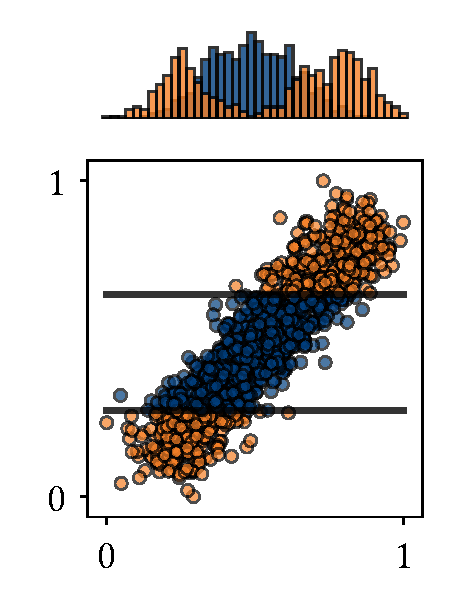
\includegraphics[width=0.241\textwidth]{part2-figures/mixed_1_2D_homo1-compressed.pdf}}
	\end{subfigure}
	\begin{subfigure}[Categorical]
			{\label{fig:slicing-categorical}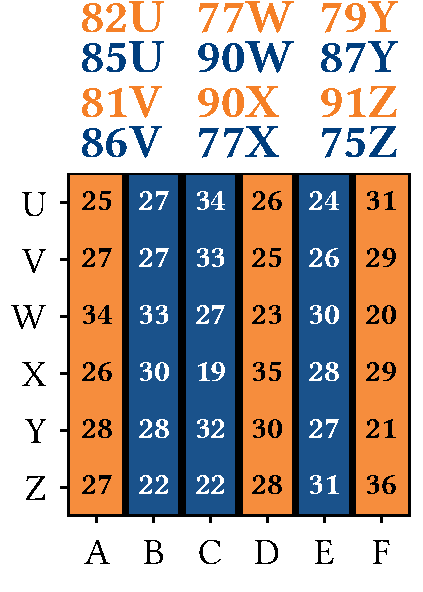
\includegraphics[width=0.241\textwidth]{part2-figures/mixed_0_2D_homo2-compressed-crop.pdf}}
	\end{subfigure} 
	\begin{subfigure}[Heterogeneous i.]
			{\label{fig:slicing-hetero1}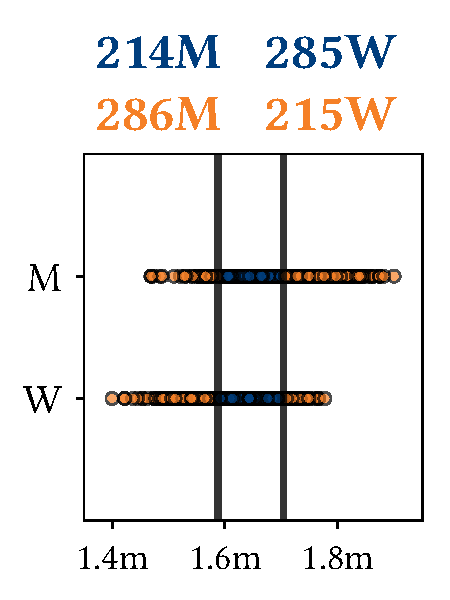
\includegraphics[width=0.241\textwidth]{part2-figures/mixed_0_2D_hetero1-compressed.pdf}}
	\end{subfigure}
	\begin{subfigure}[Heterogeneous ii.]
			{\label{fig:slicing-hetero2}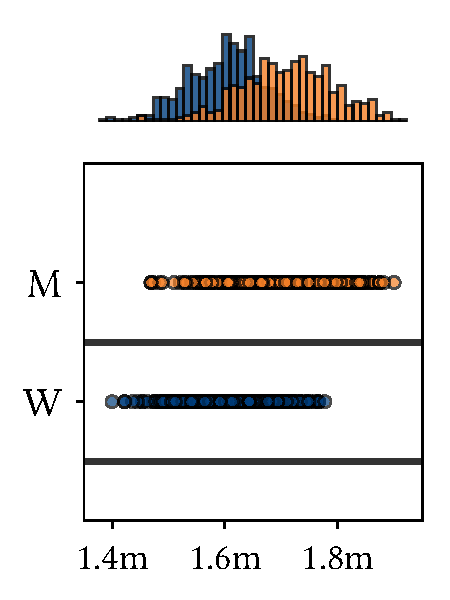
\includegraphics[width=0.241\textwidth]{part2-figures/mixed_1_2D_hetero2-compressed.pdf}}

	\end{subfigure} 
	\caption{Slicing in numerical, categorical, and heterogeneous subspaces ($|\gls{S}|=2$).} 
	\label{fig:slicing}
\end{figure} 

We illustrate slicing in heterogeneous subspaces in Figure \ref{fig:slicing}, with an exemplary numerical and categorical subspace in the left half and a heterogeneous subspace in the right half. 
The black lines show a random slice. The points in dark blue are in $c_i$, and the points in light orange are in $\overline{c}_i$. 
Figure \ref{fig:slicing-numerical} represents a numerical linear dependency. We can see from the histograms that, after slicing, the distribution of the points in each sample are very different. 
Figure \ref{fig:slicing-categorical} depicts the absolute frequencies of observing various symptoms $\{U \dots Z\}$ in different groups of patients $\{A \dots F\}$. 
Since there is no ordering within symptoms and patient groups, slicing in this case consists in selecting categories at random, here $\{B, C, E\}$. By comparing the absolute frequencies after slicing, we can determine whether there is a statistical association between groups and symptoms. 
Naturally, the statistical test that we use to estimate the discrepancy between $p_{s_i | {\overline{c}_i}}$ and $p_{s_i | {c_i}}$ might differ depending on the type of the reference attribute, as we will discuss later.  %This illustrate the major difference between slicing in a numerical or categorical space. 

Different attribute types can also be part of the same subspace, as we show in Figure \ref{fig:slicing-hetero1} and \ref{fig:slicing-hetero2}. We graph the height from a sample of individuals of two sexes. 
When we slice on the $x$-axis, the slice is a numerical interval. 
On the $y$-axis in turn, the slice is a category drawn at random. 

Intuitively, ordinal attributes share features from both numerical and categorical attributes: there exists an ordering between values, but typically also many tying values. In this case, we recommend using a similar slicing methodology as for numerical attributes, by selecting a discrete interval (see Definition \ref{slice}), and a statistical test that is robust to tying values to some extent. 

\subsection{Properties of Contrast}
\label{contrastproperties}

A statistical test $\mathcal{T}\left( B_1, B_2 \right)$ for two samples $B_1$ and $B_2$ typically yields a $p$-value. 
Traditionally, one uses $p$-values to assess the \textit{statistical significance}. %It is the probability to falsely reject a true null hypothesis, where the null hypothesis is the independence. 
Conversely, $\overline{p} = 1-p$ is known as \textit{confidence level}. % or probability to truly reject a false null hypothesis. 
The rationale behind estimating the degree of dependency $\mathcal{D}^*$ is to yield values quantifying the independence violation. 
We define \textit{contrast}, abbreviated as $\mathcal{C}$, as the expected value of the \textit{confidence level} of a statistical test $\mathcal{T}$ between the samples from the conditional distributions for all the possible attributes $\gls{s_i}$ and slices $c_i$:
\begin{definition}[Contrast $\mathcal{C}$]
	\label{def:contrast-test}
	\begin{align} 
	\mathcal{C}(\gls{S}) &\equiv
	\mathop{\mathbb{E}}_{c_i \in \mathcal{P}^{c}(\gls{S})}
	\Big [ \mathcal{T} \left (B(c_i), B(\overline{c}_i) \right ) \Big ]
	\end{align} 
	where $\mathcal{T}$ yields $\overline{p}$-values, and $B(c_i), B(\overline{c}_i)$ are the samples resulting from slicing. We draw the conditions in $c_i$ randomly and independently, w.r.t. any reference attribute $\gls{s_i}$ in subspace $\gls{S}$.
\end{definition}
By definition, %and independently from the underlying test,
$\mathcal{T} \sim \mathcal{U}[0,1]$ when the two samples are independent, and $\mathcal{T} \approx 1$ as the evidence against independence increases. The properties of $\mathcal{C}$ follow:
\begin{enumerate}[noitemsep]
	\item $\mathcal{C}$ converges to $1$ as the dependency in $\gls{S}$ increases.%, since the $p^c$-values converge to $1$ stochastically.
	\item $\mathcal{C}$ converges to $0.5$ when $\gls{S}$ is independent, since $\mathcal{T} \sim \mathcal{U}[0,1]$. %the distribution of the $p^c$-values converges to  $\mathcal{U}[0,1]$.
	\item $\mathcal{C}$ is bounded between $0$ and $1$.
\end{enumerate}
\label{mcde-properties}

\subsection{Monte Carlo Approximation}
\label{montecarlosimulation}
It is impossible to compute $\mathcal{C}$ exactly; one would need to know the distribution of $B(c_i)$ and $B(\overline{c}_i)$ 
for every slice. Instead, we approximate $\mathcal{C}$ via Monte Carlo (MC) simulations, with $M$ iterations. In each iteration, we choose the reference attribute $s_i$ and slice $c_i$ at random.  
We define the \textit{approximated contrast} $\mathcal{\widehat{C}}$:  

\begin{definition}[Approximated Contrast $\mathcal{\widehat{C}}$]
	\label{def:contrast-approx}
	\begin{align} 
	\mathcal{\widehat{C}}(\gls{S}) &= 
	\frac{1}{M} \sum_{m=1}^{M} \left [ \mathcal{T} \left(B\left(c_{i}  \right), B\left(\overline{c}_i\right)\right)~:~c_{i}  \overset{m}{\sim} \mathcal{P}^c(\gls{S}) \right ]
	\end{align} 
	where $c_{i} \overset{m}{\sim} \mathcal{P}^c(\gls{S})$ means that we draw $c_i$ randomly from $\mathcal{P}^c(\gls{S})$ in iteration~$m$.
\end{definition}

\label{bound} Interestingly, we can bound the quality of the approximation. From Hoeffding's inequality \cite{doi:10.1080/01621459.1963.10500830},
we derive a bound on the probability of $\mathcal{\widehat{C}}$ to deviate not less than $\varepsilon$ from $\mathcal{C}$. The bound decreases exponentially with increasing $M$:

\begin{theorem}[Hoeffding's Bound of $\mathcal{\widehat{C}}$]
	\label{"th:hoeffding-chernoff-contrast"}
	\begin{align}
	\Pr\left[| \mathcal{\widehat{C}} - \mathcal{C} | \geq \varepsilon \right] \leq 2e^{-2M \varepsilon^2}
	\end{align}
	where $M$ is the number of MC iterations, and $0 < \varepsilon < 1 - \mathcal{C}$. 
\end{theorem} 

\begin{proof}[Proof of Theorem \ref{"th:hoeffding-chernoff-contrast"}]
	Let us first restate Theorem 1 from \cite{doi:10.1080/01621459.1963.10500830} (see also Lemma \ref{hoeffdinginequality}): 
	Let $X_1, X_2, \dots, X_n$ be independent random variables $0 \leq X_i \leq 1$ for $i=1,\dots,n$ and let $\bar{X} = \frac{1}{n}(X_1 + X_2 + \dots + X_n)$ be their mean with expected value $E[\bar{X}]$. Then, for $0<t<1-E[\bar{X}]$, it holds that $\Pr[\bar{X}-E[\bar{X}] \geq t] \leq \e^{-2nt^2}$ and $\Pr[\bar{X}-E[\bar{X}] \leq t] \leq \e^{-2nt^2}$.

	We can treat each MC iteration $m_1, \dots, m_M$ as i.i.d. random variables $X_{m_1}, \dots, X_{m_M}$ with $0 \leq X_{m_i} \leq 1$. $\mathcal{\hat{C}}$ is the mean of the iterations with $E[\mathcal{\hat{C}}] = \mathcal{C}$ (\mbox{Definition \ref{def:contrast-test}}). Thus, for $0 < \varepsilon < 1 - \mathcal{C}$ it holds that
	\begin{align}
	\Pr[\mathcal{\hat{C}}-\mathcal{C} \geq \varepsilon] \leq \e^{-2M\varepsilon^2} && \Pr[\mathcal{\hat{C}}-\mathcal{C} \leq \varepsilon] \leq \e^{-2M\varepsilon^2}
	\end{align}
	since $\Pr[|\mathcal{\hat{C}}-\mathcal{C}| \geq \varepsilon] = \Pr[\mathcal{\hat{C}}+\mathcal{C} \geq \varepsilon] + \Pr[\mathcal{\hat{C}}-\mathcal{C} \geq \varepsilon]$ it is easy to verify Theorem~\ref{"th:hoeffding-chernoff-contrast"}.
\end{proof}

This is very useful. For instance, when $M=200$, the probability of $\mathcal{\widehat{C}}$ to deviate more than $0.1$ from its expected value is less than $2e^{-4} \approx 0.04$, and this bound decreases exponentially with $M$. Thus, one can adjust the computational requirements of $\mathcal{\widehat{C}}$ given the available resources, the desired quality level, or the rate of arrival of new observations in a stream. In other words, users can set $M$ intuitively, as it leads to an expected quality, and vice versa. Observe that $M$ is our only parameter. 

\subsection{Instantiating \gls{MCDE}}
\label{sec:instantiationMCDE}

One must instantiate $\mathcal{T}$ as a suitable statistical test. Ideally, $\mathcal{T}$ is non-parametric (\hyperlink{R4}{\textbf{R4}}) and suitable for the type of the reference attribute (numerical, ordinal, categorical). To facilitate meaningful experiments, we investigate instantiations  of \gls{MCDE}  based  on  three  well-known  non-parametric  tests: the Kolmogorov-Smirnov, the Mann-Whitney U and  the Chi-Squared test. We call the respective instantiations \gls{KSP}, \gls{MWP} and \gls{CSP}. 

The Kolmogorov-Smirnov test assumes the data to be continuous, i.e., it should be adequate for numerical attributes. 
The Mann-Whitney U test specifically handles tying values, so it might work well with ordinal attributes. 
Lastly, the Chi-Squared test bases on frequencies from a finite number of categories, i.e., we hypothesise it to be suitable for categorical attributes.
\begin{algorithm}\footnotesize
	\caption{\textsc{\gls{MCDE}}$(\gls{S} = \{s_1, \dots, s_{|\gls{S}|}\})$}\label{MCDE_alg}
	\begin{algorithmic}[1]
		\State $\mathcal{I} \gets$ \textsc{ConstructIndex}{$\left(\gls{S}\right)$} ; $\textit{result} \gets 0$ \label{MCDE_alg:line1}
		\For{$m \gets 1$ to $M$}
		\State $r \gets$ random integer in $\left[ 1,|\gls{S}| \right]$ 
		\State $slice \gets$ \textsc{Slice}{$\left(\mathcal{I}, r \right)$} \label{MCDE_alg:line4}
		\State $\textit{result} \gets \textit{result } +$ \textsc{Test}{$\left( \mathcal{I} , slice, r \right)$} \label{MCDE_alg:line5}
		\EndFor
		\State {\bfseries return} $(\textit{result} / M) \in (0,1)$
	\end{algorithmic}
\end{algorithm}

Algorithm \ref{MCDE_alg} summarises the general idea behind \gls{MCDE} for any arbitrary subspace $\gls{S} = \{s_1, \dots, s_{|\gls{S}|}\}$ of dimensionality $|\gls{S}|$. 
In practice, we can significantly improve the efficiency of slicing operations, which require the values of each attribute to be ordered, with an index structure (Line \ref{MCDE_alg:line1}). Afterwards, for $M$ iterations, we slice the data (Line~\ref{MCDE_alg:line4}) and carry out the statistical test (Line \ref{MCDE_alg:line5}). %We can do this efficiently thanks to the index, because tuples are sorted. 
The final estimate is the average of the test outcomes over $M$ iterations. In what follows, we present the specifics of the procedures \textsc{ConstructIndex}, \textsc{Slice} and \textsc{Test} for each instantiation of \gls{MCDE}. 

\section{Instantiation as \acrfull{MWP}}

We first consider the instantiation of $\mathcal{T}$ as a two-sided Mann-Whitney U test \cite{Mann1947}. %, as in our previous work \cite{DBLP:conf/kdd/FoucheKB19}. 
An advantage of this test is that it does not assume the data to be continuous, as it operates on ranks. So it is robust and applicable to numeric and ordinal measurements.  

\subsection{Estimating The Mann-Whitney U Statistics} 

In a nutshell, the Mann-Whitney U test compares the difference between the median of two samples. We review the definition of this test \cite{Siegel1956} between two samples $B_1$ and $B_2$ with size $n_1$ and $n_2$, and $n_1 + n_2 = \gls{w}$. It tests the null hypothesis that it is equally likely that a randomly selected value from one sample will be less than or greater than a randomly selected value from the other sample. $R_1$ and $R_2$ are the sums of ranks of the objects in $B_1$ and $B_2$, obtained by ranking the values of $B_1$ and $B_2$ together, starting with $0$. In case of ties, the ranks of the tying objects are \textit{adjusted}, i.e., become the average of their ranks. 
\begin{align}
p = \Phi(Z)~\text{or}~1-\Phi(Z) && Z = \frac{ U_i - \mu }{\sigma} && U_i = R_i - \frac{n_i(n_i-1)}{2}
\end{align}
Here, one can choose $U_i = U_1$ or  $U_i = U_2$ equivalently. $\Phi$ is the cumulative distribution function of the normal distribution, and $\mu$, $\sigma$ are defined as: 
\begin{align}
\mu = \frac{n_1 n_2}{2} && \sigma = \sqrt{\frac{n_1 n_2}{12} \left ( (\gls{w}+1) - \sum_{i=1}^{k} \frac{t_i^3 - t_i}{\gls{w}(\gls{w}-1)} \right ) }
\end{align}
The summation term of $\sigma$ is a correction for ties, where $t_i$ is the number of observations sharing rank $i$, and $k$ is the number of distinct ranks.
Typically, for $\gls{w} > 20$, the values of $U$ are normally distributed \cite{Mann1947} with mean $\mu$ and standard deviation $\sigma$. $Z$ is the standardised score, since \mbox{$Z \sim \mathcal{N}(0,1)$}. If $U = U_1$, then $Z \ll 0$ and $p \approx 0$ when the ranks of $A_1$ are stochastically smaller than those of $A_2$. Conversely, when the ranks of $A_1$ are stochastically larger, then $Z \gg 0$ and $p \approx 1$.
Both cases indicate an independence violation. As both directions are relevant, our test should capture them equally: %That is why we use the two-sided variant of the U test: 
\begin{align}
\text{MWP} = \Phi^{1/2}(Z') && Z' = |Z| && U = U_1
\end{align}
Since $Z  \sim \mathcal{N}(0,1)$, $Z'$ follows the so-called half-normal distribution with \textit{cdf} $\Phi^{1/2}$. Since $|U_1 - \mu|$ = $|U_2 - \mu|$, we can simply set $U = U_1$ or $U = U_2$ arbitrarily.%, i.e., one only needs to sum the ranks of one of the samples.

However, the ability of this test to detect dependency --  the `power' -- declines in the case of unequal variance of the two samples \cite{zimmerman2003warning, fagerland2009wilcoxon}. %This effect becomes problematic in case of unequal variance between marginal and conditional distributions. 
Thus, we include an additional step into the slicing process. 
It restricts the domain of the reference attribute $\gls{s_i}$ to a share $\alpha$ of observations. Formally, we define the marginal restriction as follows: 

\begin{definition}[Marginal Restriction]
	A marginal restriction is a condition on the reference attribute $\gls{s_i}$, i.e., an interval $r_i:[l_{i}, u_{i}]$ or $r_i:[l_{i} \dots u_{i}]$, so that $|\{ \vec{\gls{x}}_j : x_{ji} \in r_i \} | = \left \lceil \alpha \cdot \gls{w} \right \rceil = \left \lceil w' \right \rceil$ and the subspace slice becomes $c_i \cup r_i$.
\end{definition}

\begin{figure}
	\centering
	\hfill
	\begin{subfigure}[without MR]
		{\label{fig:circle-nomarginal}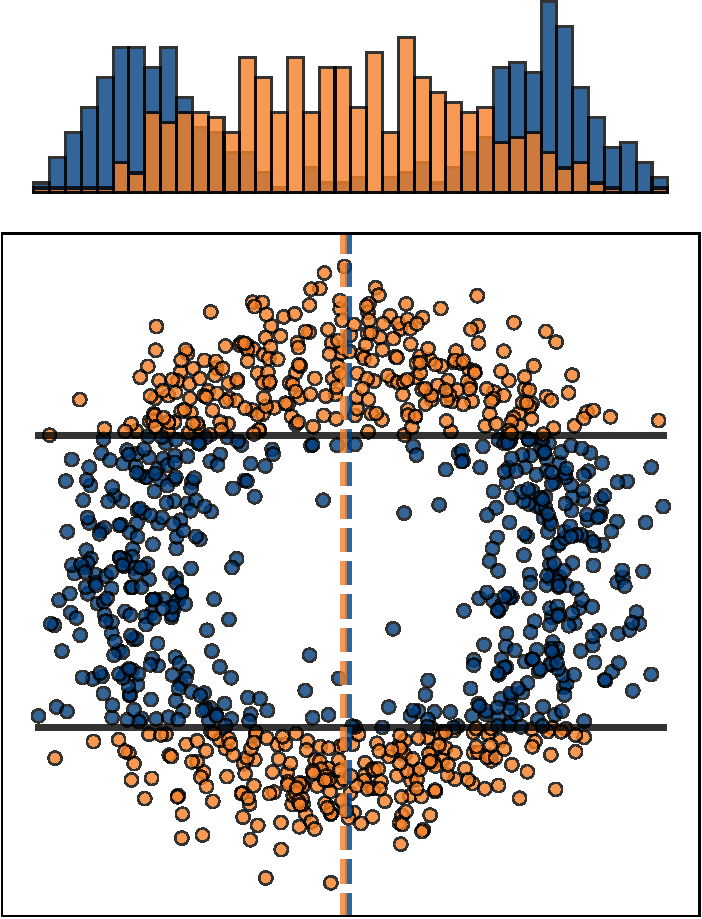
\includegraphics[width=0.21\textwidth]{part2-figures/circle_2D_0_nomarginal-crop-compressed.pdf}}
	\end{subfigure}
	\hfill
	\begin{subfigure}[with MR]
		{\label{fig:circle-marginal}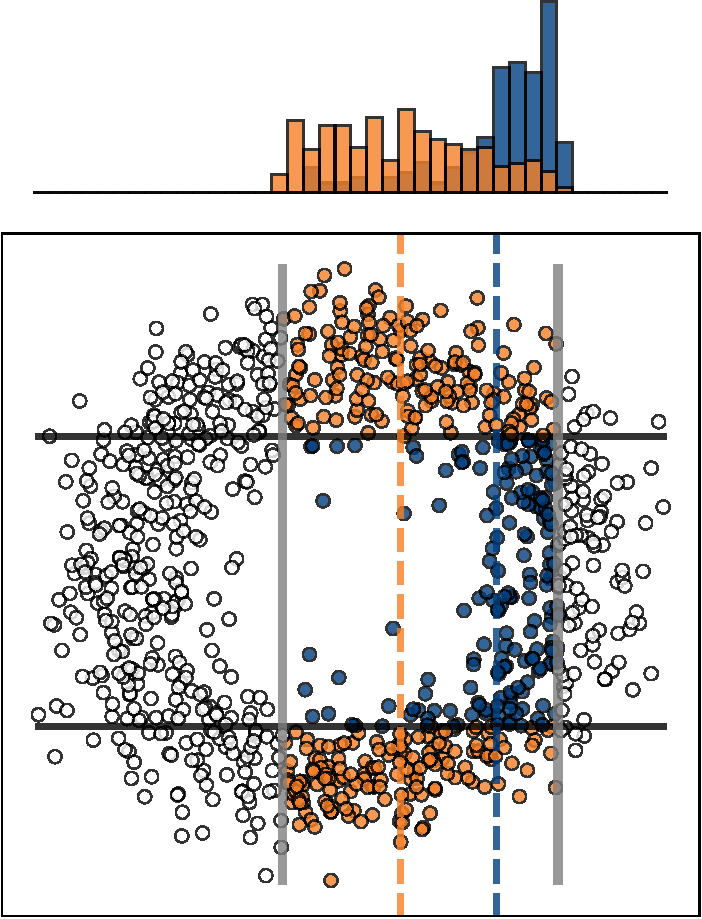
\includegraphics[width=0.21\textwidth]{part2-figures/circle_2D_0_marginal-crop-compressed.pdf}}
	\end{subfigure} 
	\hfill
	\begin{subfigure}[without MR]
		{\label{fig:linear-nomarginal}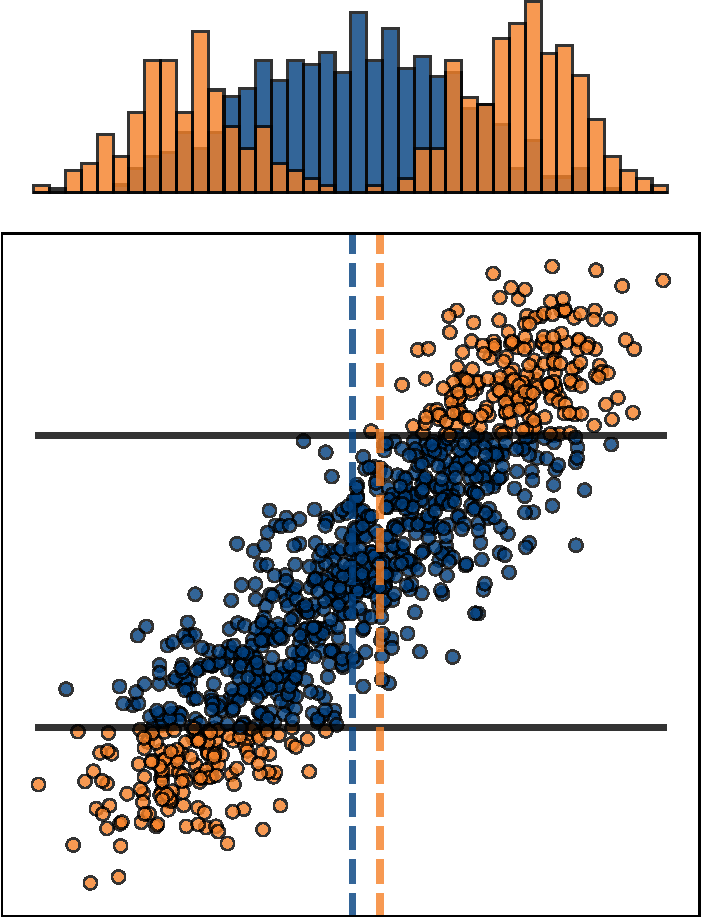
\includegraphics[width=0.21\textwidth]{part2-figures/linear_2D_0_nomarginal-crop-compressed.pdf}}
	\end{subfigure}
	\hfill
	\begin{subfigure}[with MR]
		{\label{fig:linear-marginal}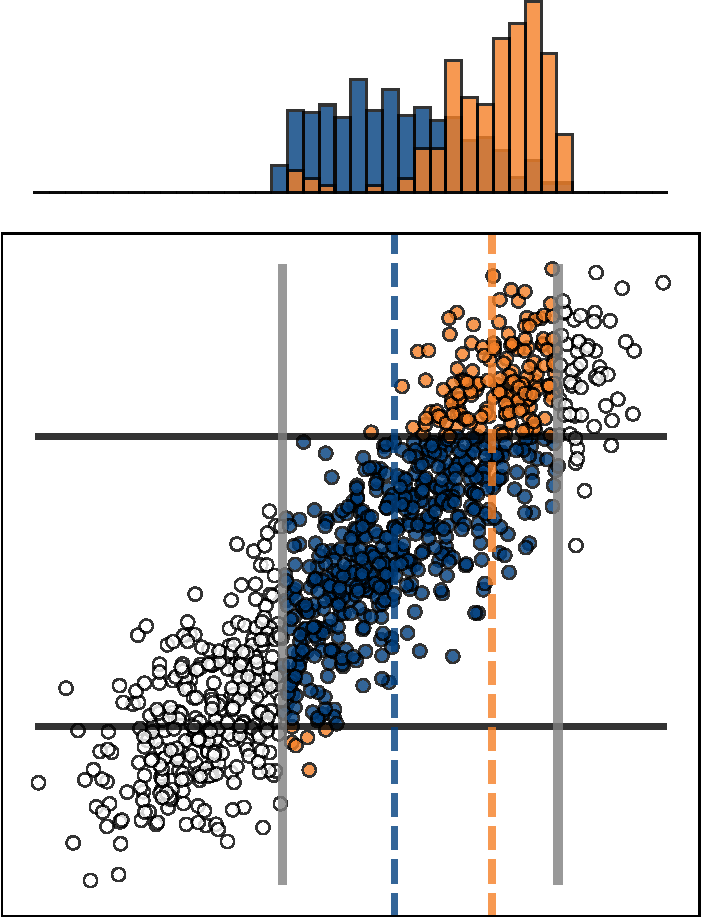
\includegraphics[width=0.21\textwidth]{part2-figures/linear_2D_0_marginal-crop-compressed.pdf}}
	\end{subfigure} 
	\hfill
	\caption{Marginal Restriction (MR) w.r.t. a circular and linear dependency ($|\gls{S}|=2$).} 
	\label{fig:slicing-marginal}
\end{figure}
We illustrate in Figure \ref{fig:slicing-marginal} the impact of the marginal restriction. 
We show in the left half a circular dependency and in the other half a linear dependency. 
Two grey lines show a marginal restriction (in \ref{fig:circle-marginal} and \ref{fig:linear-marginal}), and two vertical dashed lines stand for the median of each sample. 
%After slicing, both samples have highly unequal variance (see \ref{fig:circle-nomarginal} and \ref{fig:linear-nomarginal}). 
%However, in \ref{fig:circle-nomarginal}, the median of both distributions are nearly equal. Thus, this dependency remains undetected. 
We can see that in both cases, the marginal restriction leads to the median of the two samples having a larger difference. Thus, the discrepancy between both samples will be better detected by the Mann Whitney U test.
%The marginal restriction solves this problem, as we see in \ref{fig:circle-marginal}.  
%However, there is almost no difference between \ref{fig:linear-nomarginal} and \ref{fig:linear-marginal}. 
Intuitively, the marginal restriction `breaks the symmetry' between both distributions. 
Because of that, the MWP estimator with marginal restriction generally has higher statistical power.

\subsection{Implementation Details}
Algorithm \ref{indexconstruction} is the pseudo-code for the index construction. The index $\mathcal{I}$ is a 1-dimensional structure containing the adjusted ranks and tying value corrections for each attribute. It consists of $|\gls{S}|$ elements $\{I_1, \dots, I_{|\gls{S}|} \}$, where $I_i$ is an array of $4$-tuples sorted by $\gls{s_i}$ in ascending order.  
In this index, $l_i$ is the row numbers, $\tilde{x}_{i}$ are the sorted values
of $\gls{s_i}$, $a_i$ are the \textit{adjusted} ranks 
and $b_i$ the accumulated correction terms of the standard deviation $\sigma$.
$I_i[j]$ stands for the $j$-th tuple of $I_i$, and $l_{ji}$, $\tilde{x}_{ji}$, $a_{ji}$, $b_{ji}$ are its components.

Algorithm \ref{mwpslice} shows the slicing process. We can slice the input data efficiently because the tuples are already sorted in the index structure. 
We successively mask the row numbers based on a random condition for all but one reference attribute $s_r$. Additionally, we ensure that the condition boundaries do not split any tying values and that each condition has exactly $w'$ observations. 
The algorithm returns a $\mathit{slice}$, i.e., a list of $\gls{w}$ Boolean values, so we write $\mathit{slice} \in \mathbb{Z}_2^{\gls{w}}$. Since we visit each value at most once, the complexity is in  $O(|\gls{S}| \cdot\gls{w})$.

Algorithm \ref{TMWP} implements the statistical test based on our index. We determine a restriction $[\mathit{start}, \mathit{end}]$ on $s_{r}$ and sum the adjusted ranks of the observations in the slice. 
%Thanks to the marginal restriction, we compute the statistical test in a subsample of size $n' < n$. 
Since the ranks in this subset may not start from $0$, we adjust the sum of the ranks $R_1$ (Line \ref{adjustranks}). Then we compute a correction (Line \ref{corrects}) using the cumulative correction $b_r$ to adjust $\sigma$ for ties (Line \ref{tieshandling}). $\Phi^{1/2}$ is the cumulative distribution function of the half-Gaussian distribution.  
We compute the statistical test via a single pass, considering only elements between $\mathit{start}$ and $\mathit{end}$. Each operation requires constant time; The complexity is in $O(\gls{w})$.

\begin{algorithm}[ht]\footnotesize
	\caption{ \textsc{\gls{MWP}-ConstructIndex}$(\gls{S} = \{s_1, \dots, s_{|\gls{S}|}\})$}\label{indexconstruction}
	%\footnotesize
	\begin{algorithmic}[1]
		\For{$i = 1$ to $|\gls{S}|$} 
		
		\State $r_i \gets \left[0,\dots,\gls{w}-1\right]$
		\State $(l_i,\tilde{x}_i) \gets$ sort $(r_i, x_i)$ by $s_i$ in ascending order, break ties randomly
		\State $I_i \gets \left[(l_{1i}, \tilde{x}_{1i}, r_{1i}),\dots,(l_{wi}, \tilde{x}_{wi}, r_{wi})\right]$ %\COMMENT{Initialise $I_i:(l^i, r^i)$}
		\State $j \gets 1$ ; $\mathit{correction} \gets 0$
		\While{$j \leq \gls{w}$}
		\State $k \gets j$ ; $t \gets 1$ ; $\mathit{adjust} \gets 0$
		\While{$(k < \gls{w}-1) \wedge (s_{i}[l_{ki}] = s_{i}[l_{k+1,i}])$}
		\State $\mathit{adjust} \gets \mathit{adjust} + r_{ki}$ ; increment $k$ and $t$
		\EndWhile
		\If{$k > j$} %\COMMENT{Adjust the rank and correction}
		\State $\mathit{adjusted} \gets (\mathit{adjust} + r_{ki}) / t$ ; $\mathit{correction} \gets \mathit{correction} + t^3 - t$ 
		\State {\bfseries for} $m \gets j$ to $k$ {\bfseries do} $I_i[m] \gets (l_{mi}, \tilde{x}_{mi}, \mathit{adjusted}, \mathit{correction})$
		\EndIf
		\State {\bfseries else} $~~I_i[j] \gets (l_{ji}, \tilde{x}_{ji}, r_{ji}, \mathit{correction})$
		
		\State $j \gets j + t$
		\EndWhile
		
		\EndFor
		\State {\bfseries return} $\mathcal{I}: \{I_1, \dots, I_{|\gls{S}|} \}$ with $I_i: (l_i, \tilde{x}_i, a_i, b_i)$
	\end{algorithmic}
\end{algorithm}

\begin{algorithm}[ht]\footnotesize
	\caption{\textsc{\gls{MWP}-Slice}{$(\mathcal{I}: \{I_1, \dots, I_{|\gls{S}|} \}, r \in \{1,\dots,|\gls{S}|\})$}}\label{mwpslice} 
	\begin{algorithmic}[1]
		\State $w' \gets \left \lceil \gls{w} \cdot \sqrt[|\gls{S}|-1]{\alpha}\,  \right \rceil  $
		\For{$I_i \in \mathcal{I} \setminus I_{r}$} 
		\State $\mathit{slice}_i \gets$ Array of $\gls{w}$ Boolean values initialised to $\mathit{false}$
		\State $\mathit{start} \gets$ random integer in $[1,\gls{w}-w']$
		\State $\mathit{end} \gets$ $\mathit{start} + w'$
		\State {\bfseries while} $r_{\mathit{start},i} = r_{\mathit{start}-1,i}$ {\bfseries do} $\mathit{start} = \mathit{start} -1$
		\State {\bfseries while} $r_{\mathit{end},i} = r_{\mathit{end}+1,i}$ {\bfseries do} $\mathit{end} = \mathit{end} + 1$
		\State {\bfseries for} $j \gets \mathit{start}$ to $\mathit{end}$  {\bfseries do} $\mathit{slice}[l_{ji}] \gets \mathit{true}$
		
		\If{$\mathit{end} - \mathit{start} > w'$}
		\State $nb \gets \mathit{end} - \mathit{start} - w'$
		\State $\mathit{exclude} \gets$ draw $nb$ sample from $[\mathit{start}, \mathit{end}]$ without replacement
		\State {\bfseries for} $el \in \mathit{exclude}$ {\bfseries do} $\mathit{slice}[el] \gets \mathit{false}$
		\EndIf
		
		\EndFor
		\State $\mathit{slice}_r \gets$ Array of $\gls{w}$ Boolean values initialised to $\mathit{true}$
		\State $\mathit{slice} \gets \mathit{slice}_1 \wedge \dots \wedge \mathit{slice}_{|\gls{S}|}$
		\State {\bfseries return} $\mathit{slice} \in \mathbb{Z}_2^{\gls{w}}$
	\end{algorithmic}
\end{algorithm}

\begin{algorithm}[ht]\footnotesize
	\caption{\textsc{\gls{MWP}-Test}{$( \mathcal{I}: \{I_1, \dots, I_{|\gls{S}|} \}, \mathit{slice} \in \mathbb{Z}_2^{\gls{w}}, r \in \{1,\dots,|\gls{S}|\})$}}\label{TMWP}
	%\footnotesize
	\begin{algorithmic}[1]
		\State $\mathit{start} \gets$ random integer in $[1,\gls{w} \cdot (1-\alpha)]$ 
		\State $\mathit{end} \gets$ $\mathit{start} + \left \lceil \gls{w} \cdot \alpha \right \rceil$
		
		\State $R_1 \gets 0$ ; $n_1 \gets 0$
		\For{$j \gets \mathit{start}$ to $\mathit{end}$} 
		\If{$\mathit{slice}[l_{jr}] = \mathit{true}$}
		\State $R_1 \gets R_1 + a_{jr}$ 
		\State $n_1 \gets n_1 + 1$
		\EndIf
		\EndFor
		\State{$w' \gets \mathit{end} - \mathit{start} $} %
		\State {\bfseries if} $n_1 = 0$ or $n_1 = w'$ {\bfseries return} $1$
		\State $U_1 \gets R_1 - \mathit{start} \cdot n_1$   \label{adjustranks}
		\State $n_2 \gets w' - n_1$
		\State $\mu \gets (n_1 \cdot n_2)/ 2$
		\State $\mathit{correction} \gets (b_{\mathit{end}-1,r}-b_{\mathit{start}-1,r})/(w'\cdot (w'-1))$ \label{corrects}
		\State $\sigma \gets \sqrt{((n_1 \cdot n_2)/12) \cdot {(w'+1-\mathit{correction})}}$ \label{tieshandling}
		\State {\bfseries return}  $\Phi^{1/2}(|U_1 - \mu| / \sigma) \in (0,1)$
	\end{algorithmic}
\end{algorithm}

\clearpage

\section{Instantiation as \acrfull{KSP}}
\label{sec:instantiatingKSP}

\subsection{Estimating Kolmogorov-Smirnov Statistic}

We now describe another instantiation of \gls{MCDE}, which uses the two-sample Kolmogorov-Smirnov (KS) test. 
The KS test is non-parametric, and it is widely used to test the equality of two continuous one-dimensional probability distributions. 
It is adequate in case the reference attribute is numerical. However, it is known that the KS test has less power in the presence of ties \cite{DBLP:books/daglib/0023683}. %p584
So it may not work well with ordinal attributes. 
% See the discussion from here: https://stats.stackexchange.com/questions/1047/is-kolmogorov-smirnov-test-valid-with-discrete-distributions

In a nutshell, the two-sample Kolmogorov-Smirnov statistic $D$ is the supremum of the absolute differences of the empirical cumulative distribution functions $F_{1}(x)$ and $F_{2}(x)$ of Samples $1$ and $2$ with $n_1$ and $n_2$ elements: 
\begin{equation}
    D = \sup_{x} \left | F_{1}(x) - F_{2}(x) \right |
\end{equation}
\gls{HiCS} employed this test statistic to quantify contrast. 
However, to comply with the \gls{MCDE} framework, one must first derive the corresponding $\overline{p}$-value. 
The $\overline{p}$-values are not trivial to obtain, because the distribution of $D$ does not have any known closed form, and the time required for an exact computation increases with $n_1$ and $n_2$ in particular.  
To obtain the $\overline{p}$-values, we approximate them using the asymptotic Kol\-mo\-go\-rov-Smir\-nov distribution proposed in \cite{durbin1973distribution}: 
\begin{equation}
\label{asymptotic-ks}
\Pr \left[D \sqrt{ \frac{n_1 \cdot n_2}{n_1+n_2}} \leq x\right] = 1 -2 \sum_{i=1}^{\infty} (-1)^{i -1} e^{-2i^2x^2}
\end{equation}
Empirically, we found that summing up the first $1000$ terms of the expansion provides enough accuracy, without much impact on the execution time. %EF: Alternatively, we could have a fixed tolerance 
Using this approximation is common practice within most modern statistical software, such as R \cite{R}. 

\subsection{Implementation Details}

%EF: We could also have used the java program from "Computing the Two-Sided Kolmogorov-Smirnov Distribution" (https://core.ac.uk/download/pdf/6287952.pdf)
%EF: The code from Alan somewhat correspond to the approximation that R does as well. The ks.test function use this approximation as long as n*m > 10000, (which is our case mostly). See the function pkstwo from ks.c. However, the difference is that they don't have a fixed number of iteration, but a fixed tolerance (which is maybe nicer?). They refer to J. Durbin (1973), Distribution Theory for Tests Based on the Sample Distribution Function.  SIAM.
%EF: The other method which I implemented is exact (as long as there is no tie), it copies methods psmirnov2x and what it does is explained here: https://r.789695.n4.nabble.com/ks-test-The-two-sample-two-sided-Kolmogorov-Smirnov-test-with-ties-PR-13848-td923859.html
%EF: Found also here: https://stat.ethz.ch/pipermail/r-devel/2009-July/054106.html
%EF: I wonder whether we need to detail both alternatives (the exact the approximate one). Ideally, it would be nicer to have the approximation with a fixed tolerance (say 1e-6 or even 1e-3).  
%EF: I appears that "Marsaglia's algorithm" is for the exact computation of the one-sample test. It is also implemented in ks.c. However, "Computing the Two-Sided Kolmogorov-Smirnov Distribution" (https://core.ac.uk/download/pdf/6287952.pdf) argue that it is slow. 
%EF: Find the ks.c source in the R sources at /src/library/stats/src/ks.c
%EF: Statsexchange discussion: https://stats.stackexchange.com/questions/149595/ks-test-how-is-the-p-value-calculated
%Optional: The importance to break ties arbitrarily?

Algorithm \ref{kspconstructindex} is the pseudo-code for the index construction. The difference to \gls{MWP} is that we do not need to adjust ranks or precompute tie correction, because the Kolmogorov-Smirnov test assumes that there are no tying values. 
The resulting data structure contains the indices $l_i$ and the values $x_i$ of each attribute $\gls{s_i}$, ordered by $\gls{s_i}$ in ascending order. 

\begin{algorithm}\footnotesize
	\caption{ \textsc{\gls{KSP}-ConstructIndex}$(\gls{S} = \{s_1, \dots, s_{|\gls{S}|}\})$}\label{kspconstructindex}
	%\footnotesize
	\begin{algorithmic}[1]
		\For{$i = 1$ to $|\gls{S}|$} 
		
		\State $r_i \gets \left[0,\dots,\gls{w}-1\right]$
		\State $(l_i,\tilde{x}_i) \gets$ sort $(r_i, x_i)$ by $\gls{s_i}$ in ascending order, break ties randomly
		\State $I_i \gets \left[(l_{1i}, \tilde{x}_{1i}),\dots,(l_{wi}, \tilde{x}_{wi})\right]$ 
		\EndFor
		\State {\bfseries return} $\mathcal{I}: \{I_1, \dots, I_{|\gls{S}|} \}$ with $I_i: (l_i, \tilde{x}_i)$
	\end{algorithmic}
\end{algorithm}

Similarly, Algorithm \ref{kspslicing} is responsible for slicing, but does not require any further step to handle ties. Algorithms \ref{indexconstruction} and \ref{kspconstructindex} as well as Algorithms \ref{mwpslice} and \ref{kspslicing} respectively behave in the same way whenever the data does not have ties. 

\begin{algorithm}\footnotesize
	\caption{\textsc{\gls{KSP}-Slice}{$(\mathcal{I}: \{I_1, \dots, I_{|\gls{S}|} \}, r \in \{1, \dots, |\gls{S}|\})$}}\label{kspslicing}
	%\footnotesize
	\begin{algorithmic}[1]
		\State $w' \gets \left \lceil \gls{w} \cdot \sqrt[|\gls{S}|-1]{\alpha}\,  \right \rceil  $
		\For{$I_i \in \mathcal{I} \setminus I_{r}$} 
		\State $\mathit{slice}_i \gets$ Array of $\gls{w}$ Boolean values initialised to $\mathit{false}$
		\State $\mathit{start} \gets$ random integer in $[1,\gls{w}-w']$
		\State $\mathit{end} \gets$ $\mathit{start} + w'$
		\State {\bfseries for} $j \gets \mathit{start}$ to $\mathit{end}$  {\bfseries do} $\mathit{slice}[l_{ji}] \gets \mathit{true}$
		\EndFor
		\State $\mathit{slice}_r \gets$ Array of $\gls{w}$ Boolean values initialised to $\mathit{true}$
		\State $\mathit{slice} \gets \mathit{slice}_1 \wedge \dots \wedge \mathit{slice}_{|\gls{S}|}$
		\State {\bfseries return} $\mathit{slice} \in \mathbb{Z}_2^{\gls{w}}$
	\end{algorithmic}
\end{algorithm}

Algorithm \ref{KSPtest} implements the KS test. We compute the statistic $D$, i.e., the largest difference of the two empirical cumulative distribution functions in Lines \ref{start-computing-D}--\ref{end-computing-D}. 
Then we approximate the $\overline{p}$-value with Equation \ref{asymptotic-ks} in Line \ref{ks-approx}. 

% Scala code to pseudecode notation
% ref.length: n
% indexSelection: slice 
% reference: r 
% inSlice: n1
% outSlice: n2
% selectIncrement: u 
% refIncrement: v
% acc1: Zeta_1 
% acc2: Zeta_2
% currentMax: D
% summation: Phi

\begin{algorithm}\footnotesize
    \caption{\textsc{\gls{KSP}-Test}{$( \mathcal{I}: \{I_1, \dots, I_{|\gls{S}|} \}, \mathit{slice} \in \mathbb{Z}_2^{\gls{w}}, r \in \{1,\dots,|\gls{S}|\} )$}}\label{KSPtest}
    \begin{algorithmic}[1]
        \State $n_1 \gets \left|\{ i: i \in [1\dots \gls{w}] \wedge \mathit{slice}[l_{ir}] = \textit{true} \}\right|$ % Nb of elements being $true$ in $slice$
        \State $n_2 \gets \gls{w} - n_1$ 

        \State {\bfseries if} $n_1 = 0$  {\bfseries or} $n_2 = 0$ {\bfseries return} $1$
        \State $u \gets 1/n_1$ ; $v \gets 1/n_2$
        \State $\zeta_1 \gets 0$ ; $\zeta_2 \gets 0$
        \State $D \gets 0 ; \phi \gets 0$ 
        \For{$i \gets 1$ to $\gls{w}$} \label{start-computing-D}
            \State {\bfseries if} $\mathit{slice}[l_{ir}] = true$ {\bfseries then} $\zeta_1 \gets \zeta_1 + u $
            \State {\bfseries else} $\zeta_2 \gets \zeta_2 + v $
            \State $D \gets max \{D, |\zeta_2 - \zeta_1| \}$
        \EndFor \label{end-computing-D}
        \State $z \gets D \sqrt{n_1 n_2 / (n_1 + n_2)}$
        \State {\bfseries for} $i \gets 1$ to $1000$ {\bfseries do} $\phi \gets \phi + (-1)^{i-1}e^{-2i^2z^2}$ \label{ks-approx}
        \Return $(1 - 2 \phi) \in (0,1)$
    \end{algorithmic}
\end{algorithm}

\section{Instantiation as \acrfull{CSP}}

\subsection{Estimating Chi-Squared Statistic}

The Chi-Squared test, also known as Pearson's Chi-Squared test, perhaps is the most famous non-parametric test. In short, it determines whether there is a significant difference between the expected frequencies and the observed frequencies of a set of categories. 

For a reference variable $\gls{s_i} \in \mathit{\gls{Cat}}$ with categories $A = \{a_1, \dots, a_{|A|}\}$, we sketch the contingency table w.r.t.\ the two samples $B(c_i)$ and $B(\overline{c}_i)$ in Table~\ref{tab:contingencytable}, where $o^i_j$ is the absolute frequency of Category $a_{j}$ in Sample $i$, and we have:
\begin{align}
    \sum_{i=1}^{|A|}{o^j_i} &= o^j && j \in \{1,2\} \\
\sum_{j=1}^{2}{o^j_i} &= o_i && i \in \{1, \dots, |A|\} 
\end{align}
\begin{table}
\caption{Exemplary Contingency Table.}
\label{tab:contingencytable}
\centering
\renewcommand{\arraystretch}{1.3}
\begin{tabular}{lccccc}
\toprule
                    & $a_1$ & $a_2$ & \dots & $a_{|A|}$      & Total \\
\midrule
Sample 1: $B(c_i)$         & $o^1_{1}$ & $o^1_{2}$ & \dots & $o^1_{{|A|}}$ & $o^1$ \\
Sample 2: $B(\overline{c}_i)$ & $o^2_{1}$ & $o^2_{2}$ & \dots & $o^2_{{|A|}}$ & $o^2$ \\
Total                       & $o_{1}$   & $o_{2}$   & \dots & $o_{{|A|}}$   & $\gls{w}$  \\
\bottomrule
\end{tabular}
\end{table}
Then we can compute the test statistic $Q$ as follows:
\begin{equation}
    Q = \sum_{i=1}^{|A|}\sum_{j=1}^{2} \frac{(o_i^j-e_i^j)^2}{e_i^j}
\end{equation}
where $e_i^j = o_i \cdot o^j / \gls{w}$ 
is the expected absolute frequency. 

Under independence, $Q$ follows the $\chi^2$ distribution with cumulative distribution function $\chi^2_k: \mathbb{R}^+ \mapsto [0,1]$, where $k = |A|-1$ is the number of degrees of freedom. Thus, $\chi^2_k(Q)$ leads to the $\overline{p}$-value that we use for \gls{CSP}. 

\subsection{Implementation Details}

As with the other instantiations, we improve the execution time with an index. It contains the position of each occurrence of a categorical value binned into its respective category. 
Algorithm \ref{cspconstructindex} is our pseudo-code for its construction. We can construct the index in linear time with a single pass over each attribute, as it does not require any sorting.

Algorithm \ref{cspslicing} is our slicing procedure for \gls{CSP}. The main difference to \gls{MWP} and \gls{KSP} is that the index is not ordered. Thus, slicing consists in selecting a random set of categories per attribute. The algorithm ensures that exactly $w'$ observations are part of each condition.

Finally, Algorithm \ref{CSPtest} shows how to compute the Chi-Squared statistic, based on the information from the index and a subspace slice. 

\subsection{Complexity}

The overall complexity of \gls{MWP} and \gls{KSP} is in $O(|\gls{S}| \cdot (\gls{w} \cdot log(\gls{w}) + \gls{w}) + M \cdot(|\gls{S}| \cdot \gls{w} + \gls{w}))$. Since $|\gls{S}| \ll \gls{w}$, this simplifies to $O(\gls{w} \cdot log(\gls{w}) + M\cdot \gls{w})$. The index construction is asymptotically the most expensive step, as it is in $O(\gls{w} \cdot log(\gls{w}))$. Since the index construction for CSP does not require sorting, this step simplifies to $O(\gls{w})$. 
However, one only needs to construct the index once for a given data set or window. When the index is available, one can compute the estimator in linear time for the exponential number of subspaces. 

Interestingly, \gls{MCDE} is trivial to parallelise: one can compute the elements of the index structure $I_1, \dots, I_{|\gls{S}|}$ in parallel, as they are independent of each other. Similarly, one can parallelise each Monte Carlo iteration. This is useful, as multi-core architectures are ubiquitous in modern database systems. 
Thus, \gls{MCDE} scales well with the size of the data set. We will verify this claim via experiments in Section \ref{sec:scalability}.

\begin{algorithm}\footnotesize
	\caption{ \textsc{\gls{CSP}-ConstructIndex}$(\gls{S} = \{s_1, \dots, s_{|\gls{S}|}\})$}\label{cspconstructindex}
	%\footnotesize
	\begin{algorithmic}[1]
		\For{$i = 1$ to $|\gls{S}|$} 
		\State Define $I_i$ as a mapping of categories to  $\left\{\mathit{positions} \subset \{0,\dots, \gls{w}-1\}, \mathit{counts} \in  \mathbb{N}^+\right\}$
		\For{$x_{ji} \in \gls{s_i}$}
		\If{$I_i[x_{ji}] \neq \emptyset$}
		\State $I_i[x_{ji}] \gets \left\{ I_i[x_{ji}].\mathit{positions} \oplus x, I_i[x_{ji}].\mathit{counts} + 1 \right\}$
		\Else
		\State   $I_i[x_{ji}] \gets \left\{j, 1 \right\}$
		\EndIf
		\EndFor
		\EndFor
		\State {\bfseries return} $\mathcal{I}: \{I_1, \dots, I_{|\gls{S}|} \}$ where $I_i: el \in \gls{s_i} \mapsto \mathbb{N}^+$
	\end{algorithmic}
\end{algorithm}

\begin{algorithm}\footnotesize
	\caption{\textsc{\gls{CSP}-Slice}{$(\mathcal{I}: \{I_1, \dots, I_{|\gls{S}|} \}, r \in \{1,\dots,|\gls{S}|\})$}}\label{cspslicing}
	%\footnotesize
	\begin{algorithmic}[1]
		\State $w' \gets \left \lceil \gls{w} \cdot \sqrt[d-1]{\alpha}\,  \right \rceil  $
		\For{$I_i \in \mathcal{I} \setminus I_{r}$} 
		\State $\mathit{slice}_i \gets$ Array of $\gls{w}$ Boolean values initialised to $\textit{false}$
		\State $\mathit{slicesize} \gets 0$ 
		\State $\mathit{positions} \gets \emptyset$
		\State $\mathit{categories} \gets \mathcal{I}_i.\mathit{keys}$
		\While{$\mathit{slicesize} < w'$}
		\State $\mathit{category} \gets $ draw a random category from $\mathit{categories}$
		\State $\mathit{categories} \gets \mathit{categories} \setminus \mathit{category}$
		\State $\mathit{slicesize} \gets \mathit{slicesize} + \mathcal{I}_i[\mathit{category}].\mathit{counts}$
		\State $\mathit{positions} \gets \mathit{positions} \oplus \mathcal{I}_i[\mathit{category}].\mathit{positions}$
		\EndWhile
		\If{$\mathit{slicesize} > w'$}
		\State Delete $\mathit{slicesize}-w'$ random elements from $\mathit{positions}$
		\EndIf
		\For{$\mathit{pos} \in \mathit{positions}$}
		\State $\mathit{slice}_i[\mathit{pos}] \gets \mathit{true}$
		\EndFor
		\EndFor
		\State $\mathit{slice}_r \gets$ Array of $\gls{w}$ Boolean values initialised to $\mathit{true}$
		\State $\mathit{slice} \gets \mathit{slice}_1 \wedge \dots \wedge \mathit{slice}_{|\gls{S}|}$
		\State {\bfseries return} $\mathit{slice} \in \mathbb{Z}_2^{\gls{w}}$
	\end{algorithmic}
\end{algorithm} 

\begin{algorithm}\footnotesize
    \caption{\textsc{\gls{CSP}-Test}{$( \mathcal{I}: \{I_1, \dots, I_{|\gls{S}|} \}, \mathit{slice} \in \mathbb{Z}_2^{\gls{w}}, r \in \{1,\dots,|\gls{S}|\} )$}}\label{CSPtest}
    \begin{algorithmic}[1]
        \State $Q = 0$ ; $k = 0$
        \State $o^1 =  |\{\mathit{pos} \in [0\dots \gls{w}-1] : \mathit{slice}[\mathit{pos}] = true\}|$
        \State $o^2 = \gls{w} - o_1$
        \For{$\{\mathit{positions}, \mathit{counts}\} \in I_r$}
        \State $o_x^1 = |\{\mathit{pos} \in \mathit{positions} : \mathit{slice}[\mathit{pos}] = \mathit{true}\}|$
        \State $o_x^2 = \mathit{counts} - o_x^1$
        \State $o_x = o_x^1 + o_x^2$
        \State $e_x^1 = o_x \cdot o^1 / \gls{w}$
        \State $e_x^2 = o_x \cdot o^2 / \gls{w}$
        \State $k = k + 1$
        \State $Q = Q + (o_x^1 - e_x^1)^2 / e_x^1 + (o_x^2 - e_x^2)^2 / e_x^2$
        \EndFor
        \Return $\chi^2_{k-1}(Q) \in (0,1)$
    \end{algorithmic}
\end{algorithm}

\clearpage

\section{\gls{MCDE} in Heterogeneous Data Streams}

\subsection{Heterogeneity}

For simplicity, we have described \gls{KSP}, \gls{MWP} and \gls{CSP}, assuming a homogeneous data set, being numerical, ordinal and categorical respectively. 

In fact, each attribute is treated independently in each of our algorithms. So we can easily extend Algorithm \ref{MCDE_alg} to the heterogeneous setting, as we show in Algorithm \ref{Heterogeneous_MCDE_alg}. We construct the index of each attribute depending on its type (Lines \ref{Heterogeneous_MCDE_indexstart}--\ref{Heterogeneous_MCDE_indexend}) and use the corresponding slicing methodology (Lines \ref{Heterogeneous_MCDE_slicingstart}-\ref{Heterogeneous_MCDE_slicingend}). 
The resulting slice is the element-wise conjunction for each type (Line \ref{Heterogeneous_MCDE_sliceconjunction}). 
The type of the reference attribute determines which test we should use (Lines \ref{Heterogeneous_MCDE_teststart}-\ref{Heterogeneous_MCDE_testend}). 
Independently of the underlying statistical test, the $\overline{p}$-values have the properties described in Section \ref{mcde-properties}. 
So the final \gls{MCDE} score is the average of the $\overline{p}$-values over each iteration.

\begin{algorithm}\footnotesize
	\caption{\textsc{Heteorogeneous-\gls{MCDE}} $( \gls{S} = \{s_1, \dots, s_{|\gls{S}|}\})$}\label{Heterogeneous_MCDE_alg}
	\begin{algorithmic}[1]
		\State $\mathcal{I}_N \gets$ \textsc{\gls{KSP}-ConstructIndex}{$\left(\{\gls{s_i} \in \gls{S}: \gls{s_i} \in \mathit{\gls{Num}}\}\right)$} \label{Heterogeneous_MCDE_indexstart}
		\State $\mathcal{I}_O \gets$ 
		\textsc{\gls{MWP}-ConstructIndex}{$\left(\{\gls{s_i} \in \gls{S}: \gls{s_i} \in \mathit{\gls{Ord}}\}\right)$} 
		\State $\mathcal{I}_C \gets$  \textsc{\gls{CSP}-ConstructIndex}{$\left(\{\gls{s_i} \in \gls{S}: \gls{s_i} \in \mathit{\gls{Cat}}\}\right)$}  \label{Heterogeneous_MCDE_indexend}
		\State $\textit{result} \gets 0$ 
		\For{$m \gets 1$ to $M$} 
		\State $r \gets$ random integer in $\left[ 1,|\gls{S}| \right]$ 
		\State $\mathit{slice}_{N} \gets$ \textsc{\gls{KSP}-Slice}{$\left( \mathcal{I}_{N}, r \right)$} \label{Heterogeneous_MCDE_slicingstart}
		\State $\mathit{slice}_{O} \gets$ \textsc{\gls{MWP}-Slice}{$\left( \mathcal{I}_{O}, r \right)$}
		\State $\mathit{slice}_{C} \gets$ \textsc{\gls{CSP}-Slice}{$\left( \mathcal{I}_{C}, r \right)$} \label{Heterogeneous_MCDE_slicingend}
		\State $\mathit{slice} \gets$ $\mathit{slice}_{N} \oplus \mathit{slice}_{O} \oplus \mathit{slice}_{C} $ \label{Heterogeneous_MCDE_sliceconjunction}
		\State {\bfseries if} $s_r \in \mathit{\gls{Num}}$ {\bfseries do} $\textit{result} \gets \textit{result } +$ \textsc{\gls{KSP}-Test}{$\left( \mathcal{I}_N , \mathit{slice}, r \right)$}  \label{Heterogeneous_MCDE_teststart}
		\State {\bfseries if} $s_r \in \mathit{\gls{Ord}}$ {\bfseries do} $\textit{result} \gets \textit{result } +$ \textsc{\gls{MWP}-Test}{$\left( \mathcal{I}_O , \mathit{slice}, r \right)$} 
		\State {\bfseries if} $s_r \in \mathit{\gls{Cat}}$ {\bfseries do} $\textit{result} \gets \textit{result } +$ \textsc{\gls{CSP}-Test}{$\left( \mathcal{I}_C , \mathit{slice}, r \right)$} \label{Heterogeneous_MCDE_testend}
		\EndFor
		\State {\bfseries return} $(\textit{result} / M) \in (0,1)$
	\end{algorithmic}
\end{algorithm}

\subsection{Adaptation to the Streaming Setting}

\label{adaptation-stream}

To deal with streams, we adopt the well-known sliding window model, i.e., we only consider the $\gls{w}$ most recent observation. A naive way to support this model is to recompute the index at the arrival of each new observation. Instead, we propose  efficient insertion and deletion operations for our indexes. 

Furthermore, to maintain a dependency estimate over time, we propose to perform a number $M$ of MC iterations periodically and report the exponential moving average: 
\begin{equation}
    \gls{MCDE}_{\gls{t}} = \gamma \cdot \gls{MCDE}(W_{\gls{t}-\Delta}) + (1-\gamma) \cdot \gls{MCDE}(\gls{W_t}) 
    \label{eq:exp-decay}
\end{equation}
where $\gamma$ is the so-called decaying factor, and $\Delta$ is the step size. 

We update the \gls{MWP} index in Algorithm \ref{indexupdate} in two steps: \textsc{Step 1: Insert/Delete} and \textsc{Step 2: Refresh}. 
Our algorithm maintains two data structures: a queue, which determines for each new point the value of the point to delete in the current window, in a first-in-first-out fashion, and a variant of our static index which supports binary search. 
In the first step, we store the values for each attribute in a queue, in chronological order. 
Then we find the positions where to insert the new point and where to delete the oldest point in the index via binary search. Then, we shift all the values to insert the point. 
In the second step, we recompute the adjusted ranks and cumulative correction as in Algorithm~\ref{indexconstruction}.

Using an adequate data structure like a binary tree, \textsc{Step 1} only has logarithmic complexity, while \textsc{Step~2} has linear complexity. 
Besides this, one must perform \textsc{Step~1} for each new point, but \textsc{Step~2} only once before slicing. 
So when re-estimating contrast only every $\Delta$-th 
step, we perform \textsc{Step~1} for each point, but \textsc{Step~2} lazily. 
As a result, we can update the index in $O(|\gls{S}| \cdot log(\gls{w}))$ in \textsc{Step~1} for each observation and postpone \textsc{Step~2}, which is in $O(|\gls{S}| \cdot \gls{w})$, to contrast estimation. Updating the \gls{KSP} index is somewhat simpler because \gls{KSP} does not handle tying values. The \gls{CSP} index is unsorted, and thus \textsc{Step~1} only requires constant time. We refer to \textsc{\gls{KSP}-Update} and \textsc{\gls{CSP}-Update} as variants of Algorithm~\ref{indexupdate} for those indexes. We summarise the complexity of each step in Table \ref{tab:complexity}.

For efficiency, Algorithm~\ref{indexupdate} simultaneously inserts and deletes observations. Note that one could also perform each operation via two independent methods. This way, one may handle time-based windows, in which observations may arrive at arbitrary time steps.%, or in batches. 

\begin{algorithm}\footnotesize
	\caption{ \textsc{\gls{MWP}-Update}$(\mathcal{I}: \{I_1, \dots, I_{|\gls{S}|} \}, \vec{\gls{x}}_{\mathit{new}} = \langle x_{\mathit{new},i} \rangle_{i \in \{1,\dots,|\gls{S}|\}})$}\label{indexupdate}
	%\footnotesize
	\begin{algorithmic}[1]
		\For{$i = 1$ to $|\gls{S}|$} 
		\State $\mathit{queue}_i.\mathit{insert}(x_{\mathit{new},i})$ ; $x_{\mathit{old},i}$ = $\mathit{queue}_i.\mathit{pop}()$ \Comment{\textsc{Step 1: Insert/Delete}}
		\State $\mathit{offset}_i$ = $\mathit{offset}_i + 1$
		\State $\mathit{insert} = \mathit{binarysearch}(I_i, x_{\mathit{new},i})$ ; $\mathit{delete} = \mathit{binarysearch}(I_i, x_{\mathit{old},i})$
		\State {\bfseries if} $\mathit{insert} < \mathit{delete}$ {\bfseries for} $x \gets \mathit{insert}$ to $\mathit{delete}$ {\bfseries do} $I_i[x+1] = I_i[x]$
		\State {\bfseries else for} $x \gets \mathit{delete}$ to $\mathit{insert}$ {\bfseries do} $I_i[x] = I_i[x+1]$
		\State $I_i[\mathit{insert}] = (\gls{w} + \mathit{offset}_i,x_{\mathit{new},i}, -1, -1)$
		\State {\bfseries for} $\mathit{pos} \gets 1$ to $\gls{w}$ {\bfseries do} $I_i[\mathit{pos}] = (l_{\mathit{pos},i}-\mathit{offset}_i,\tilde{x}_{\mathit{pos},i}, \mathit{pos}, 0)$ \Comment{\textsc{Step 2: Refresh}}
		\State $\mathit{offset}_i \gets 0$ ; $j \gets 1$ ; $\mathit{correction} \gets 0$
		\While{$j \leq \gls{w}$}
		\State $k \gets j$ ; $t \gets 1$ ; $\mathit{adjust} \gets 0$
		\While{$(k < \gls{w}-1) \wedge (s_{i}[l_{ki}] = s_{i}[l_{k+1,i}])$}
		\State $\mathit{adjust} \gets \mathit{adjust} + a_{ki}$ ; increment $k$ and $t$
		\EndWhile
		\If{$k > j$} %\COMMENT{Adjust the rank and correction}
		\State $\mathit{adjusted} \gets (\mathit{adjust} + a_{ki}) / t$ ;  $\mathit{correction} \gets \mathit{correction} + t^3 - t$ 
		\State {\bfseries for} $m \gets j$ to $k$ {\bfseries do} $I_i[m] \gets (l_{mi}, \tilde{x}_{mi}, \mathit{adjusted}, \mathit{correction})$
		\EndIf
		\State {\bfseries else} $~~I_i[j] \gets (l_{ji}, \tilde{x}_{ji}, a_{ji}, \mathit{correction})$
		\State $j \gets j + t$
		\EndWhile
		\EndFor
		\State {\bfseries return} $\mathcal{I}: \{I_1, \dots, I_{|\gls{S}|} \}$ with $I_i: (l_i, \tilde{x}_i, a_i, b_i)$
	\end{algorithmic}
\end{algorithm}

\begin{table}
\caption{Algorithmic Complexity of \gls{MCDE} instantiations.}
\label{tab:complexity}
%% local settings
\sisetup{detect-weight,mode=text}
\centering
\addtolength{\tabcolsep}{-1pt}
\centering
\small
\renewcommand{\arraystretch}{0.8}% Tighter
\begin{tabular}{lccc}
\toprule
& \gls{MWP} & \gls{KSP} & \gls{CSP} \\
\midrule
Index Construction & $O(|\gls{S}| \cdot \gls{w} \cdot log(\gls{w}))$ & $O(|\gls{S}| \cdot \gls{w} \cdot log(\gls{w}))$ & $O(|\gls{S}| \cdot \gls{w})$ \\
Slicing & $O(|\gls{S}| \cdot \gls{w})$              & $O(|\gls{S}| \cdot \gls{w})$              & $O(|\gls{S}| \cdot \gls{w})$ \\
Test & $O(\gls{w})$                      & $O(\gls{w})$                      & $O(\gls{w})$         \\
Update (\textsc{Step 1}) & $O(|\gls{S}| \cdot log(\gls{w}))$                 & $O(|\gls{S}| \cdot log(\gls{w}))$                 & $O(1)$         \\
Update (\textsc{Step 2})   & $O(|\gls{S}| \cdot \gls{w})$                      & $O(|\gls{S}| \cdot \gls{w})$                      & $O(|\gls{S}| \cdot \gls{w})$         \\
\bottomrule
\end{tabular}
\end{table}

\section{Experiments}
\label{evaluation}

\subsection{Methodology}

To evaluate our dependency estimators, i.e., \gls{MWP}, \gls{KSP}, \gls{CSP} and our competitors, we look at how they behave w.r.t.\ an assortment of dependencies. See Figure \ref{fig:deps-plot}; The dependencies are scaled to $[0,1]$. \cite{DBLP:conf/ssdbm/FoucheB19} displays in appendix our algorithms for generating each dependency. 
For benchmarking, we repeatedly draw $\gls{w}$ objects with $|\gls{S}|$ dimensions, to which we add Gaussian noise with standard deviation $\sigma$, which we call \textit{noise level}. 
Intuitively, noise-free dependencies should lead to higher scores than noisier ones. 

We also show that \gls{MCDE} handles heterogeneity by simulating numerical, ordinal, and categorical attributes. To simulate ordinal attributes, we discretise numerical attributes into a number $\Omega$ of values from $1$ to $20$. To simulate categorical attributes, we randomly permute the discretised values, to mimic the absence of an order. As in other studies \cite{DBLP:conf/sdm/NguyenMV16, Reshef1518, Kinney2013}, we compute the statistical power, defined as follows: 

\begin{definition}[Power]
	The power of an estimator $\mathcal{E}$ w.r.t.\ dependency O with $\sigma$, $\gls{w}$ and $|\gls{S}|$ is the probability of the \textit{score} of $\mathcal{E}$ to be larger than a $\gamma$-th percentile of the \textit{scores} w.r.t. the independent subspace \textup{I}:
	\begin{align*}
	\Pr\left[ \mathcal{E}\left(Inst_{\gls{w} \times |\gls{S}|}^{\textup{O},\sigma}\right) > \left \{\mathcal{E}\left(Inst_{\gls{w} \times  |\gls{S}|}^{\textup{I},0}\right) \right \}^{P_\gamma} \right]
	\end{align*} 
\end{definition}

$Inst_{\gls{w} \times |\gls{S}|}^{\text{O},\sigma}$ is a random instantiation of a subspace as dependency O with noise level $\sigma$, which has $\gls{w}$ objects and $|\gls{S}|$ dimensions. $\{x\}^{P_\gamma}$ stands for the $\gamma$-th percentile of the set $\{x\}$, i.e., a value $v$ so that $\gamma \%$ of the values in $\{x\}$ are smaller than $v$.

The attributes of the independent subspace I are i.i.d.\ in $\mathcal{U}[0,1]$. Note that, since the attributes of I are independent, adding noise does not have any effect on dependence, so we set noise to 0 when instantiating I. 
To estimate the power, we draw two sets of $500$ estimates from $\text{O}$, $\sigma$ and $\text{I}$, respectively: 
\begin{align*}
\Sigma^\mathcal{E}_{\text{O}, \sigma} : \left \{ \mathcal{E}\left(Inst_{\gls{w} \times |\gls{S}|}^{\text{O},\sigma}\right) \right \}_{i=1}^{500} ~ &&\Sigma^{\mathcal{E}}_\text{I} : \left \{ \mathcal{E}\left(Inst_{\gls{w} \times |\gls{S}|}^{\text{I},0}\right) \right \}_{i=1}^{500}
\end{align*}
Then we count the elements in $\Sigma^\mathcal{E}_{\text{O}, \sigma}$ greater than $\left \{\Sigma^{\mathcal{E}}_\text{I} \right \}^{P_\gamma}$: 
\begin{align*}
\text{power}^{\text{O},\sigma,\gamma}_{\gls{w} \times |\gls{S}|}(\mathcal{E})  = \frac{\left|\left\{x:x \in \Sigma^\mathcal{E}_{\text{O}, \sigma} ~\wedge~  x > \left \{\Sigma^{\mathcal{E}}_\text{I} \right \}^{P_\gamma}\right \}\right|}{500}
\end{align*}

One can interpret `power' as the probability to correctly reject the independence hypothesis with $\gamma \%$ confidence. I.e., the power quantifies how well a dependency measure can differentiate between the independence I and a given dependency O with noise level $\sigma$. 
For our experiments, we set $\gamma =95$, $\gls{w}=1000$. We let the noise $\sigma$ vary linearly from $0$ to $1$, with $30$ distinct levels. We consider dependencies with dimensionality $|\gls{S}|$ from $2$ to $20$.

\begin{figure}
    \begin{subfigure}[C]
			{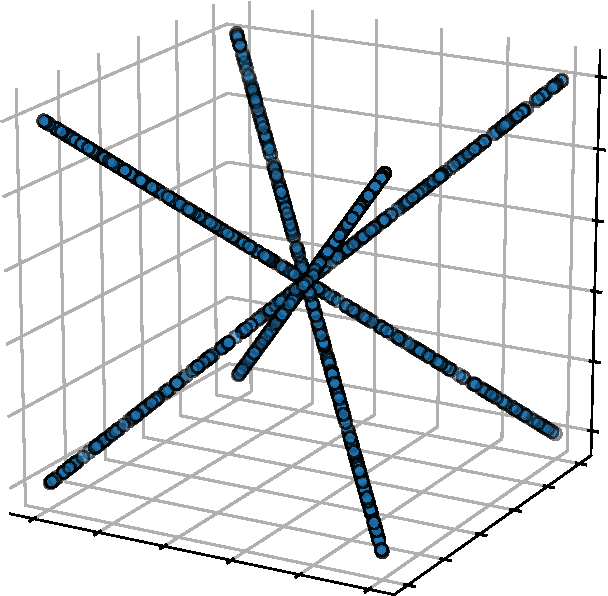
\includegraphics[width=0.14\textwidth]{part2-figures/Cross-3-00-crop-compressed.pdf}}
	\end{subfigure}
	\hfill
    \begin{subfigure}[Dl]
			{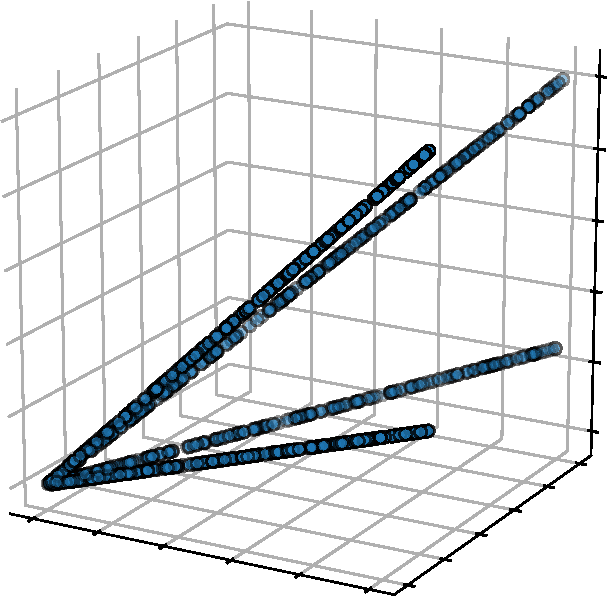
\includegraphics[width=0.14\textwidth]{part2-figures/DoubleLinear_025-3-00-crop-compressed.pdf}}
	\end{subfigure}
	\hfill
	\begin{subfigure}[H]
			{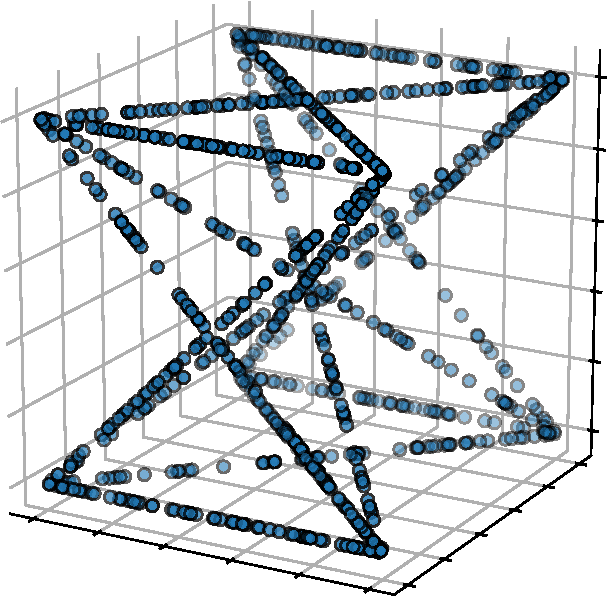
\includegraphics[width=0.14\textwidth]{part2-figures/Hourglass-3-00-crop-compressed.pdf}}
	\end{subfigure}
	\hfill
	\begin{subfigure}[Hc]
			{
			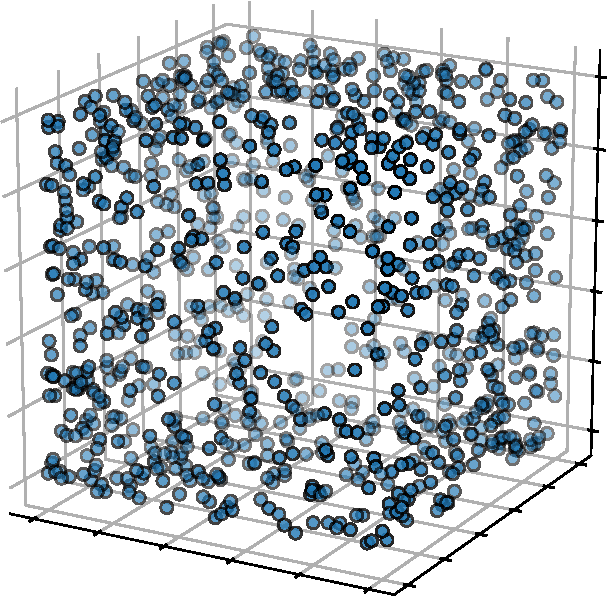
\includegraphics[width=0.14\textwidth]{part2-figures/Hypercube-3-00-crop-compressed.pdf}}
	\end{subfigure}
	\hfill
	\begin{subfigure}[HcG]
			{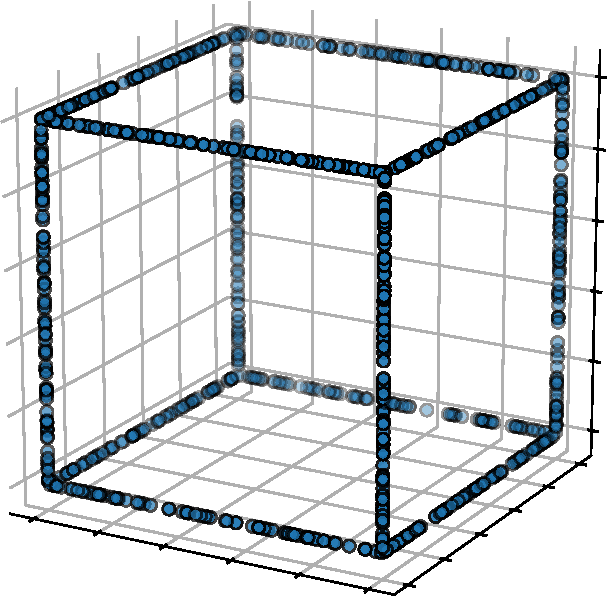
\includegraphics[width=0.14\textwidth]{part2-figures/Hollowcube-3-00-crop-compressed.pdf}}
	\end{subfigure}
	\hfill
	\begin{subfigure}[Hs]
			{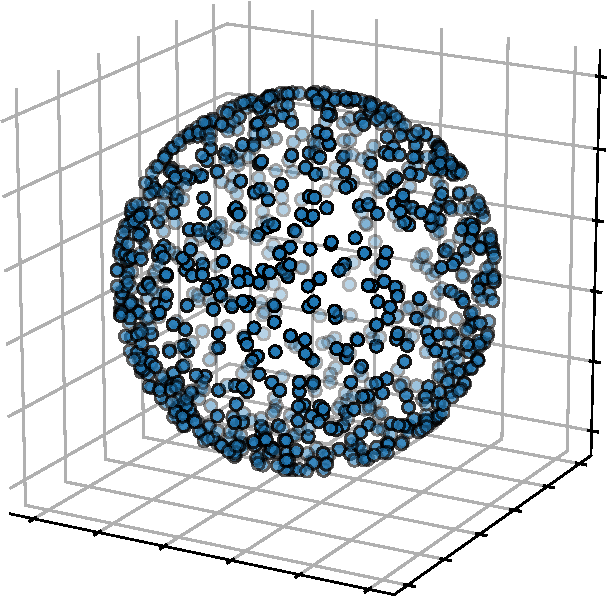
\includegraphics[width=0.14\textwidth]{part2-figures/Sphere-3-00-crop-compressed.pdf}}
	\end{subfigure} 
    
    \begin{subfigure}[L]
			{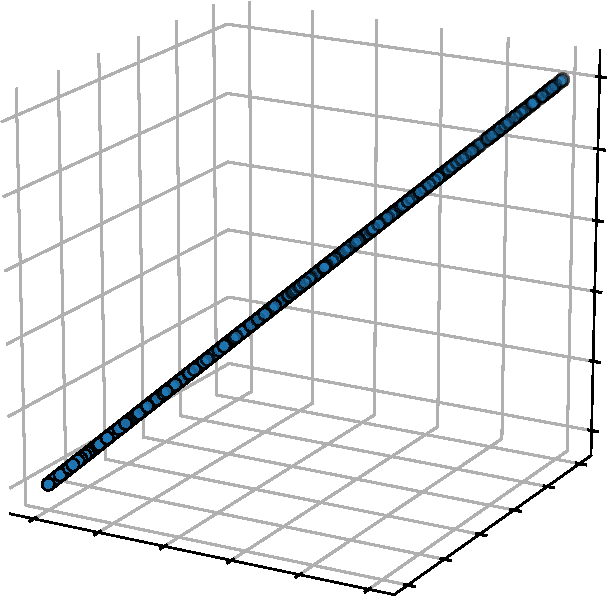
\includegraphics[width=0.14\textwidth]{part2-figures/Linear-3-00-crop-compressed.pdf}}
	\end{subfigure}
	\hfill
    \begin{subfigure}[P]
			{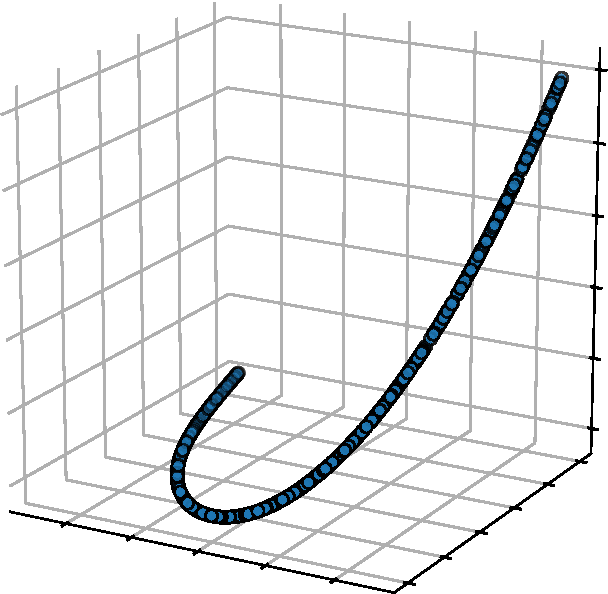
\includegraphics[width=0.14\textwidth]{part2-figures/EvenPower_1-3-00-crop-compressed.pdf}}
	\end{subfigure}
	\hfill
	\begin{subfigure}[S1]
			{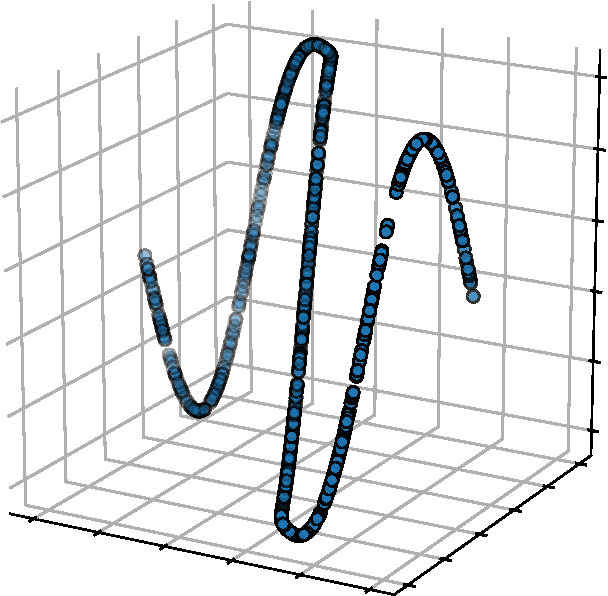
\includegraphics[width=0.14\textwidth]{part2-figures/Sine_1-3-00-crop-compressed.pdf}}
	\end{subfigure}
	\hfill
	\begin{subfigure}[S5]
			{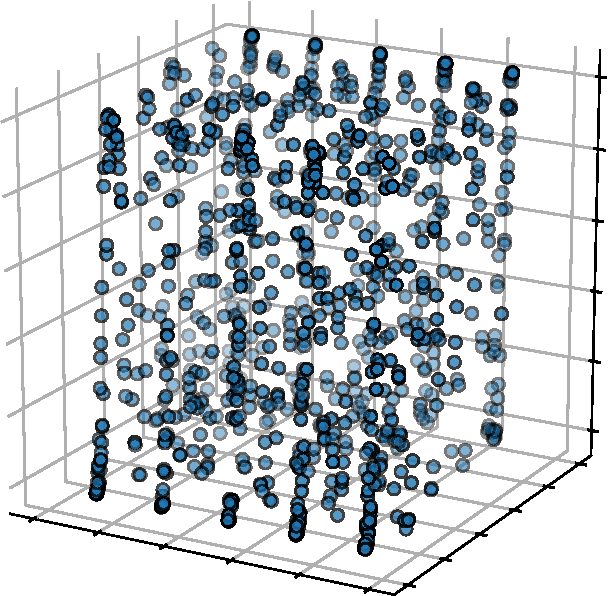
\includegraphics[width=0.14\textwidth]{part2-figures/Sine_5-3-00-crop-compressed.pdf}}
	\end{subfigure}
	\hfill
	\begin{subfigure}[St]
			{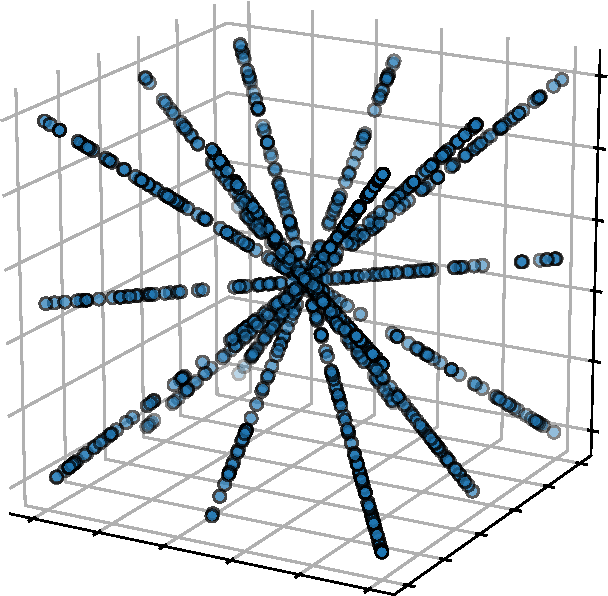
\includegraphics[width=0.14\textwidth]{part2-figures/Star-3-00-crop-compressed.pdf}}
	\end{subfigure}
	\hfill
	\begin{subfigure}[Zi]
			{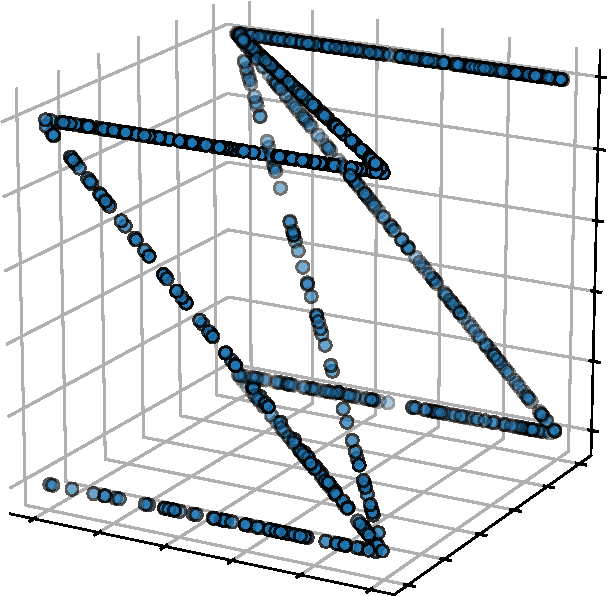
\includegraphics[width=0.14\textwidth]{part2-figures/Zinv-3-00-crop-compressed.pdf}}%\hfill
	\end{subfigure} 
	\caption{An assortment of 12 dependencies (displayed here with three dimensions, $\sigma=0$). C: Cross, Dl: Double linear, H: Hourglass, Hc: Hypercube, HcG: Hypercube Graph, Hs: Hypersphere, L: Linear, P: Parabolic, S1: Sine (P=1), S5: Sine (P=5), St: Star, Zi: Z inversed.}
	\label{fig:deps-plot}
\end{figure}

In our figures, $\text{O}_{\Omega}$ denotes each dependency, where $\text{O}$ stands for the dependency type (e.g., L stands for `Linear'), and $\Omega$ is the discretisation level, i.e., the number of distinct values; $\text{O}$ means that the attributes are numerical. 
`$|\gls{S}|$D' indicates the dimensionality, and $\text{O}^*_\Omega$ indicates that the attributes are categorical, with a number $\Omega$ of nominal values.

\subsection{Evaluation}

In our evaluation, we first compare our three estimators (\gls{MWP}, \gls{KSP} and \gls{CSP}) together. Then, we compare \gls{MWP} to our competitors and present our case study. 

\subsubsection{Specifics of Attributes Types}

We first observe how \gls{MCDE} handles numerical, ordinal, and categorical attributes. 
Figure~\ref{fig:distribution} displays the empirical distribution of \gls{MWP}, \gls{KSP} and \gls{CSP} iterations w.r.t.\ a $2$-dimensional independent (I) and a linearly dependent (L) space. 
Each distribution is estimated as a histogram from $10\,000$ independent iterations. The vertical dashed lines show the means of the distributions, and we display a scatter plot illustrating the corresponding scenario. 

According to Figure \ref{fig:distributuon-independent}, \gls{MWP}, \gls{KSP} and \gls{CSP} values are uniformly distributed in the case of an independent subspace, with a few exceptions: 
First, the \gls{CSP} values are all close to $0$ in the case of numerical attributes. 
Since each point is unique, they are all treated as a single category, 
and the Chi-Squared test does not have power in this setting. 
We observe the same effect with L (in \ref{fig:distributuon-linear}). 
Second, we see that the values of \gls{MWP} and \gls{CSP} are also $0$ with I$_1$. 
This corresponds to the desired behaviour. In this situation, every observation in the subspace is equal, so contrast is undefined. 
\gls{KSP} assumes that values are continuous, and thus does not handle this case.

Also, we can see from \ref{fig:distributuon-linear} that the \gls{KSP} values are generally closer to $1$ with L and L$_{10}$. 
This indicates a larger power than \gls{MWP} and \gls{CSP}. 
However, we can see that the \gls{CSP} distribution does not change between L$_{10}$ and L$^*_{10}$, while the mean of the \gls{MWP} and \gls{KSP} distribution decreases significantly. 
Thus, \gls{CSP} detects dependency from categorical attributes better than \gls{MWP}/\gls{KSP}. 

\begin{figure}
	\begin{subfigure}[Independent]
			{\label{fig:distributuon-independent}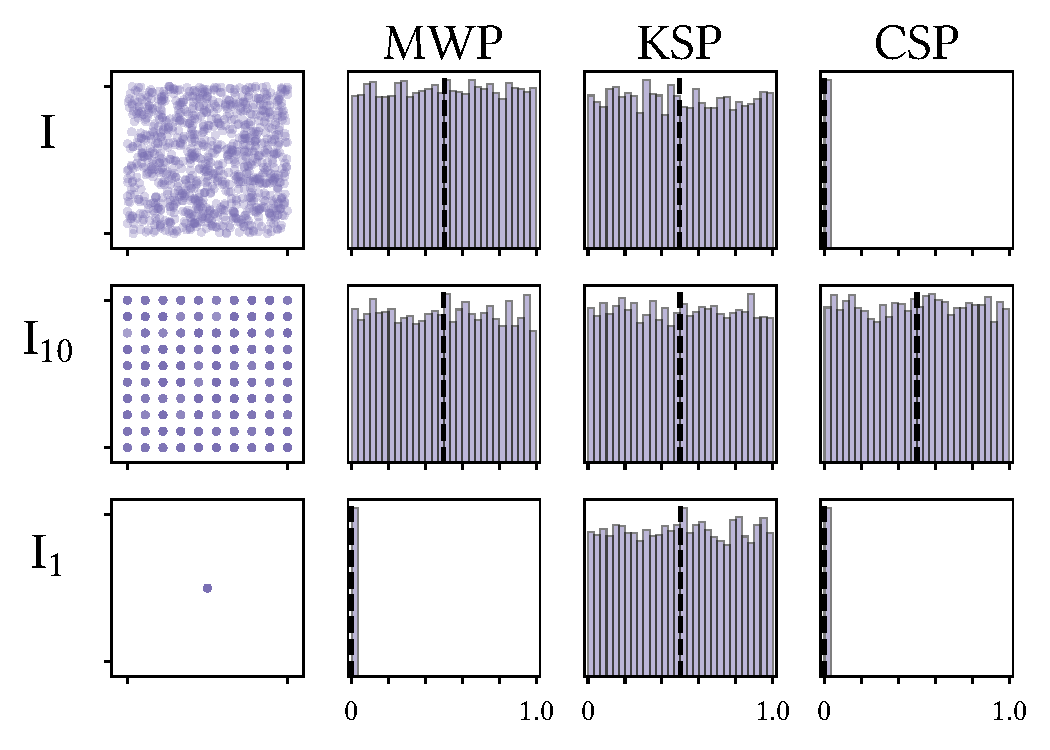
\includegraphics[width=0.49\textwidth, trim=0 0 0 0.5cm]{part2-figures/contrast_distribution_data_I_thesis-compressed.pdf}}
	\end{subfigure}
	\hfill
	\begin{subfigure}[Dependent (Linear, $\sigma=0.4$)]
			{\label{fig:distributuon-linear}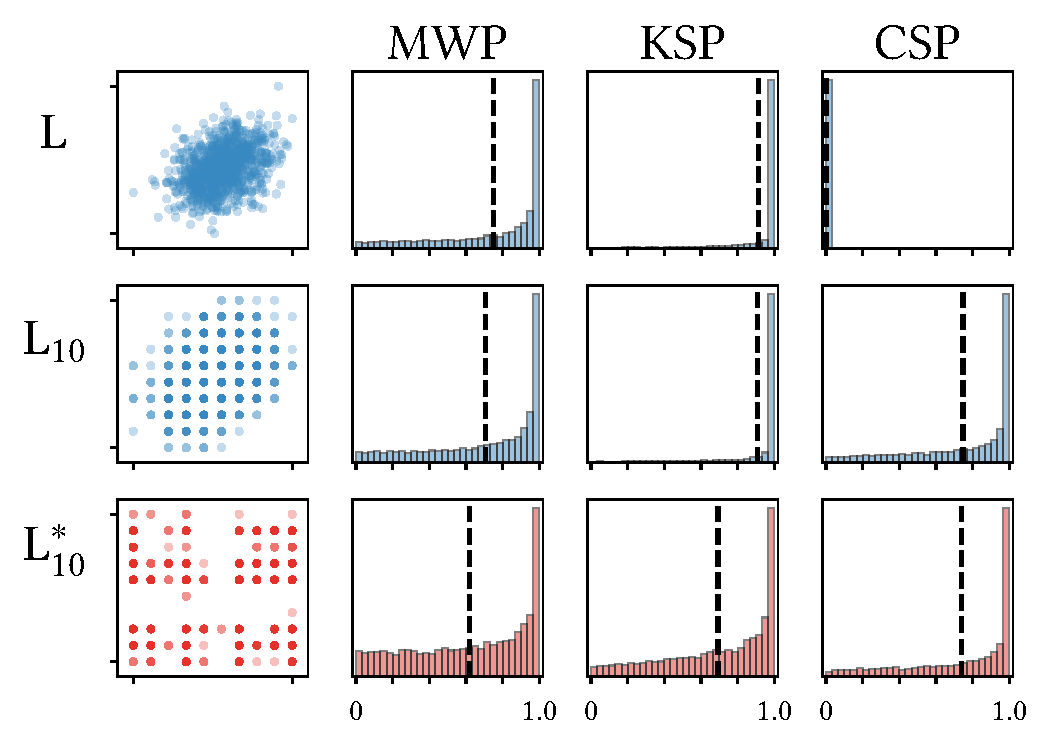
\includegraphics[width=0.49\textwidth, trim=0 0 0 0.5cm]{part2-figures/contrast_distribution_data_L_thesis-compressed.pdf}}
	\end{subfigure} 
	\caption{Distribution of the contrast estimation iterations ($|\gls{S}| = 2$).} 
	\label{fig:distribution}
\end{figure}

\subsubsection{Statistical Power of \gls{MWP}, \gls{KSP} and \gls{CSP}}

We first look at the statistical power of \gls{MWP}, \gls{KSP} and \gls{CSP} with confidence level $\gamma = 0.95$  against a linear dependency of increasing dimensionality $|\gls{S}|$, discretisation level $\Omega$, and noise level $\sigma$. 
Please note that the figures are best seen in colour. 
The expectation is that the scores and statistical power are high for noiseless dependencies, i.e., the left side of the plot is blue, and decrease gradually as we add noise. A noise level $\sigma = 1$ is comparably high since the data is scaled to $[0,1]$. Thus, the right side of the plot should be red, standing for low scores, or low power. 
From Figure \ref{fig:power} (upper part), we see that \gls{MWP} without marginal restriction does not work well in high-dimensional and highly discretised spaces. 

The marginal restriction alleviates this problem to some extent, in particular for numerical subspaces. 
In fact, as dimensionality increases, it becomes more and more likely that the points selected in the slice are `at the centre' of the distribution. 
As a result, the mean of the point in the slice and the point outside of the slice become nearly equal, leading to low power with the Mann-Whitney U test, and thus a slight performance decrease of \gls{MWP}. %In general, MWP has less power than KSP. 
This calls for further research on the \gls{MWP} slicing scheme, or alternatives to the Mann-Whitney U test. 
Nonetheless, the results indicate that \gls{MWP} with marginal restriction works well against numerical attributes. Next, we see that \gls{KSP} has high power in every case, although slightly decreasing with $\Omega$. 
\gls{CSP} does not work with numerical spaces but has more power in discrete spaces. \gls{CSP} works best with categorical attributes. 
% We also see that KSP is more robust against noise. 

We now compare the power of our estimators against the assortment of dependencies from Figure \ref{fig:deps-plot}. 
\gls{CSP} does not apply to numerical attributes. Thus, for comparability, we discretise the values with $\Omega = 10$. We can see from Figure \ref{fig:power} (lower part) that \gls{KSP} consistently has more power than \gls{MWP}, and even alleviate some of its drawbacks, such as the low power against the noiseless Hypercube (Hc). 
\gls{CSP} generally has less power than \gls{KSP} but can detect categorical dependencies. 

Our experiments show that \gls{MWP} has a slight performance decrease in high-dimensional discrete spaces. 
\gls{KSP} seems to perform better, but its statistical power decreases with discretisation. 
Overall, we recommend to use \gls{KSP} for numerical and ordinal data but to use \gls{CSP} for categorical data. 
\gls{MWP} still is a valid alternative with numerical attributes. %In the future, it would be interesting to come up with better subspace slicing schemes for MWP. 

\begin{figure}
	\centering 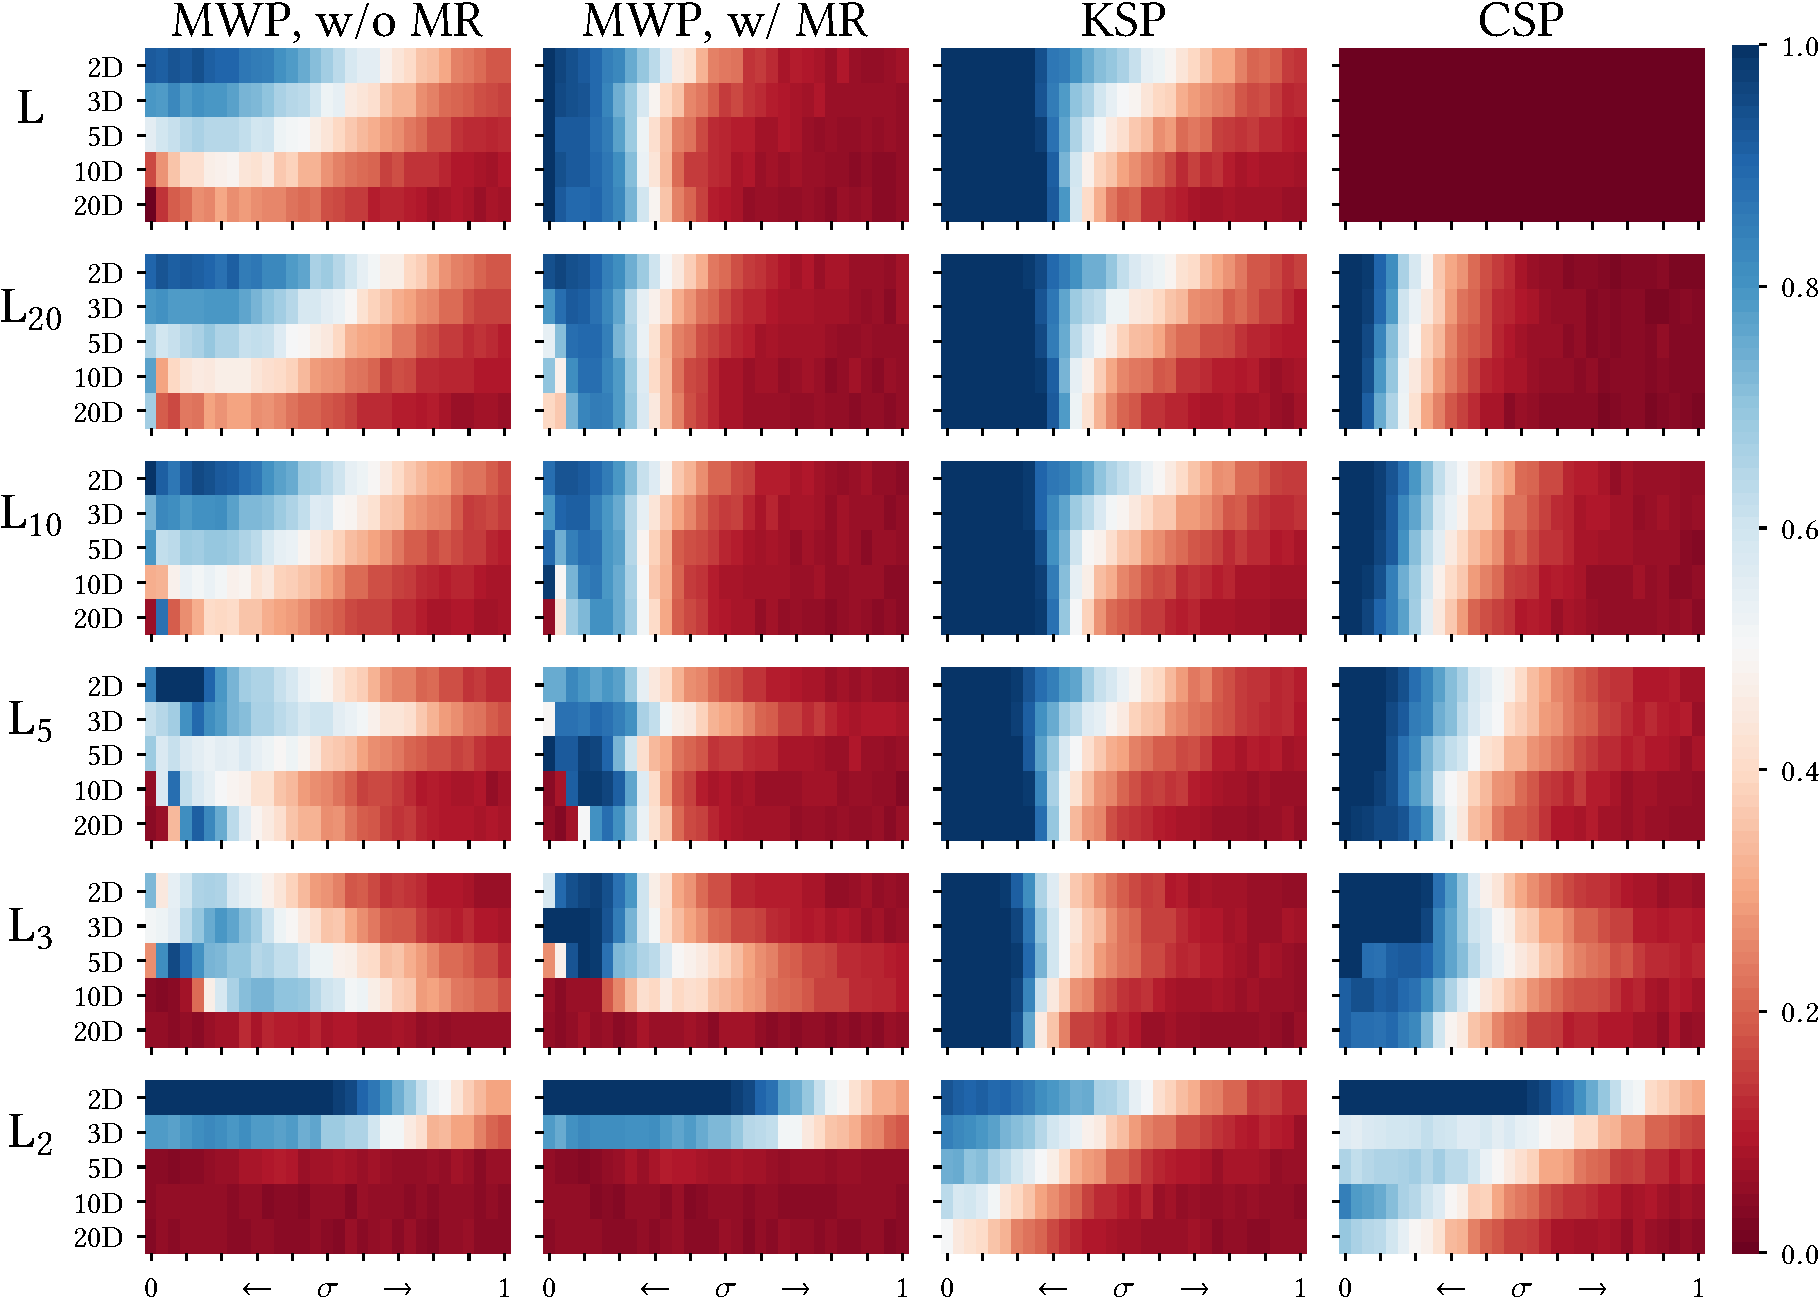
\includegraphics[width=0.98\linewidth, trim=0 0.25cm 0 0.25cm]{part2-figures/power_L_thesis-crop-compressed.pdf} \hfill \\
	\vfill
	\hfill
	\vfill
    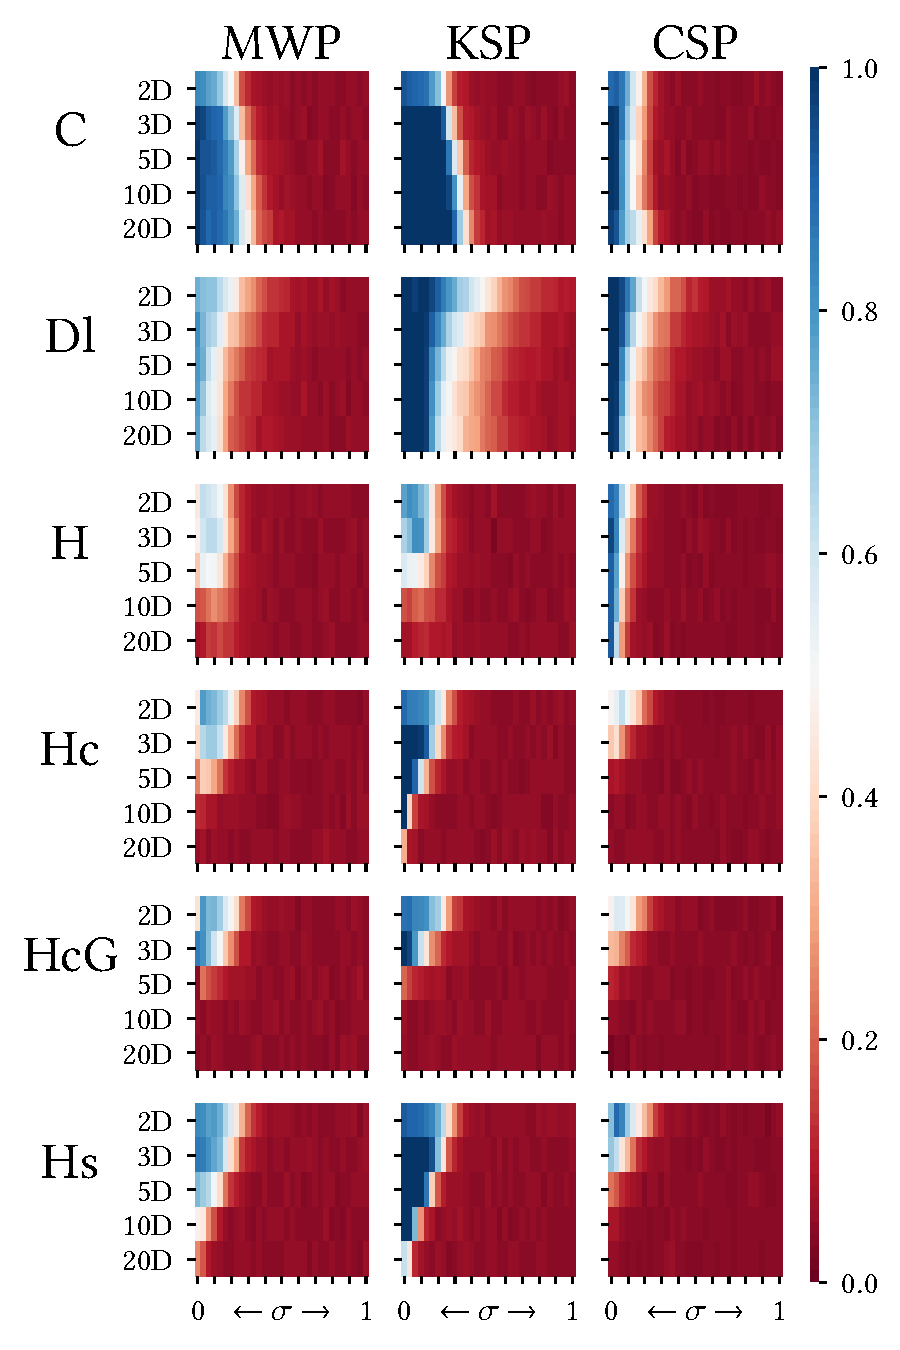
\includegraphics[width=0.49\linewidth, trim=0 0.25cm 0 0.25cm]{part2-figures/power_1_thesis-compressed.pdf}
    \hfill
    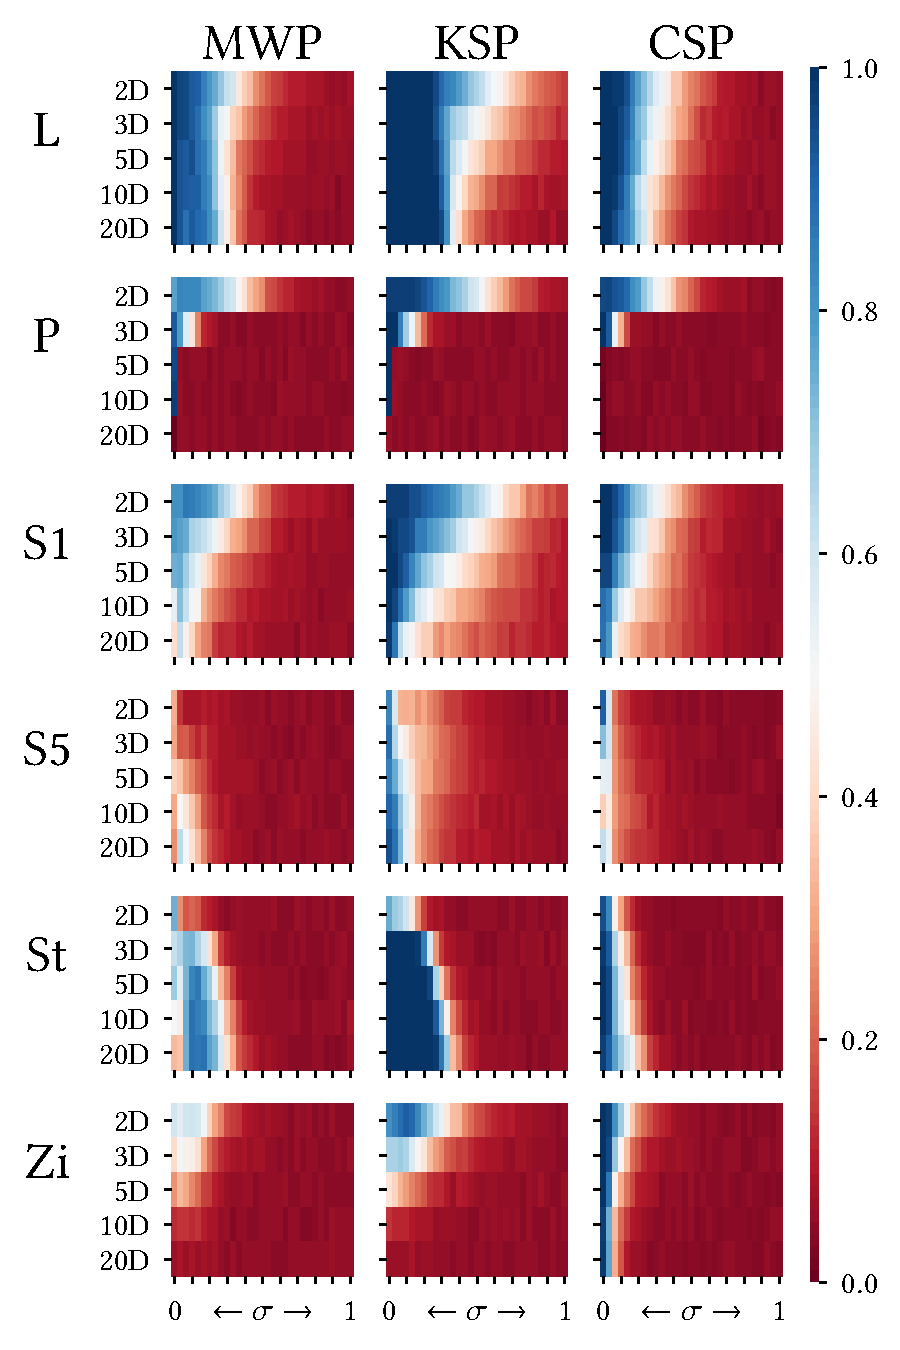
\includegraphics[width=0.49\linewidth, trim=0 0.25cm 0 0.25cm]{part2-figures/power_2_thesis-compressed.pdf}
    \hfill
    \caption{Power of \gls{MWP}/\gls{KSP}/\gls{CSP} against continuous/discrete linear distributions (upper part) and our assortment of dependencies (lower part).}
    \label{fig:power}
\end{figure} 

\subsubsection{Influence of parameters, $\gls{w}$, $M$ and $|\gls{S}|$}

\begin{figure}
	\centering
	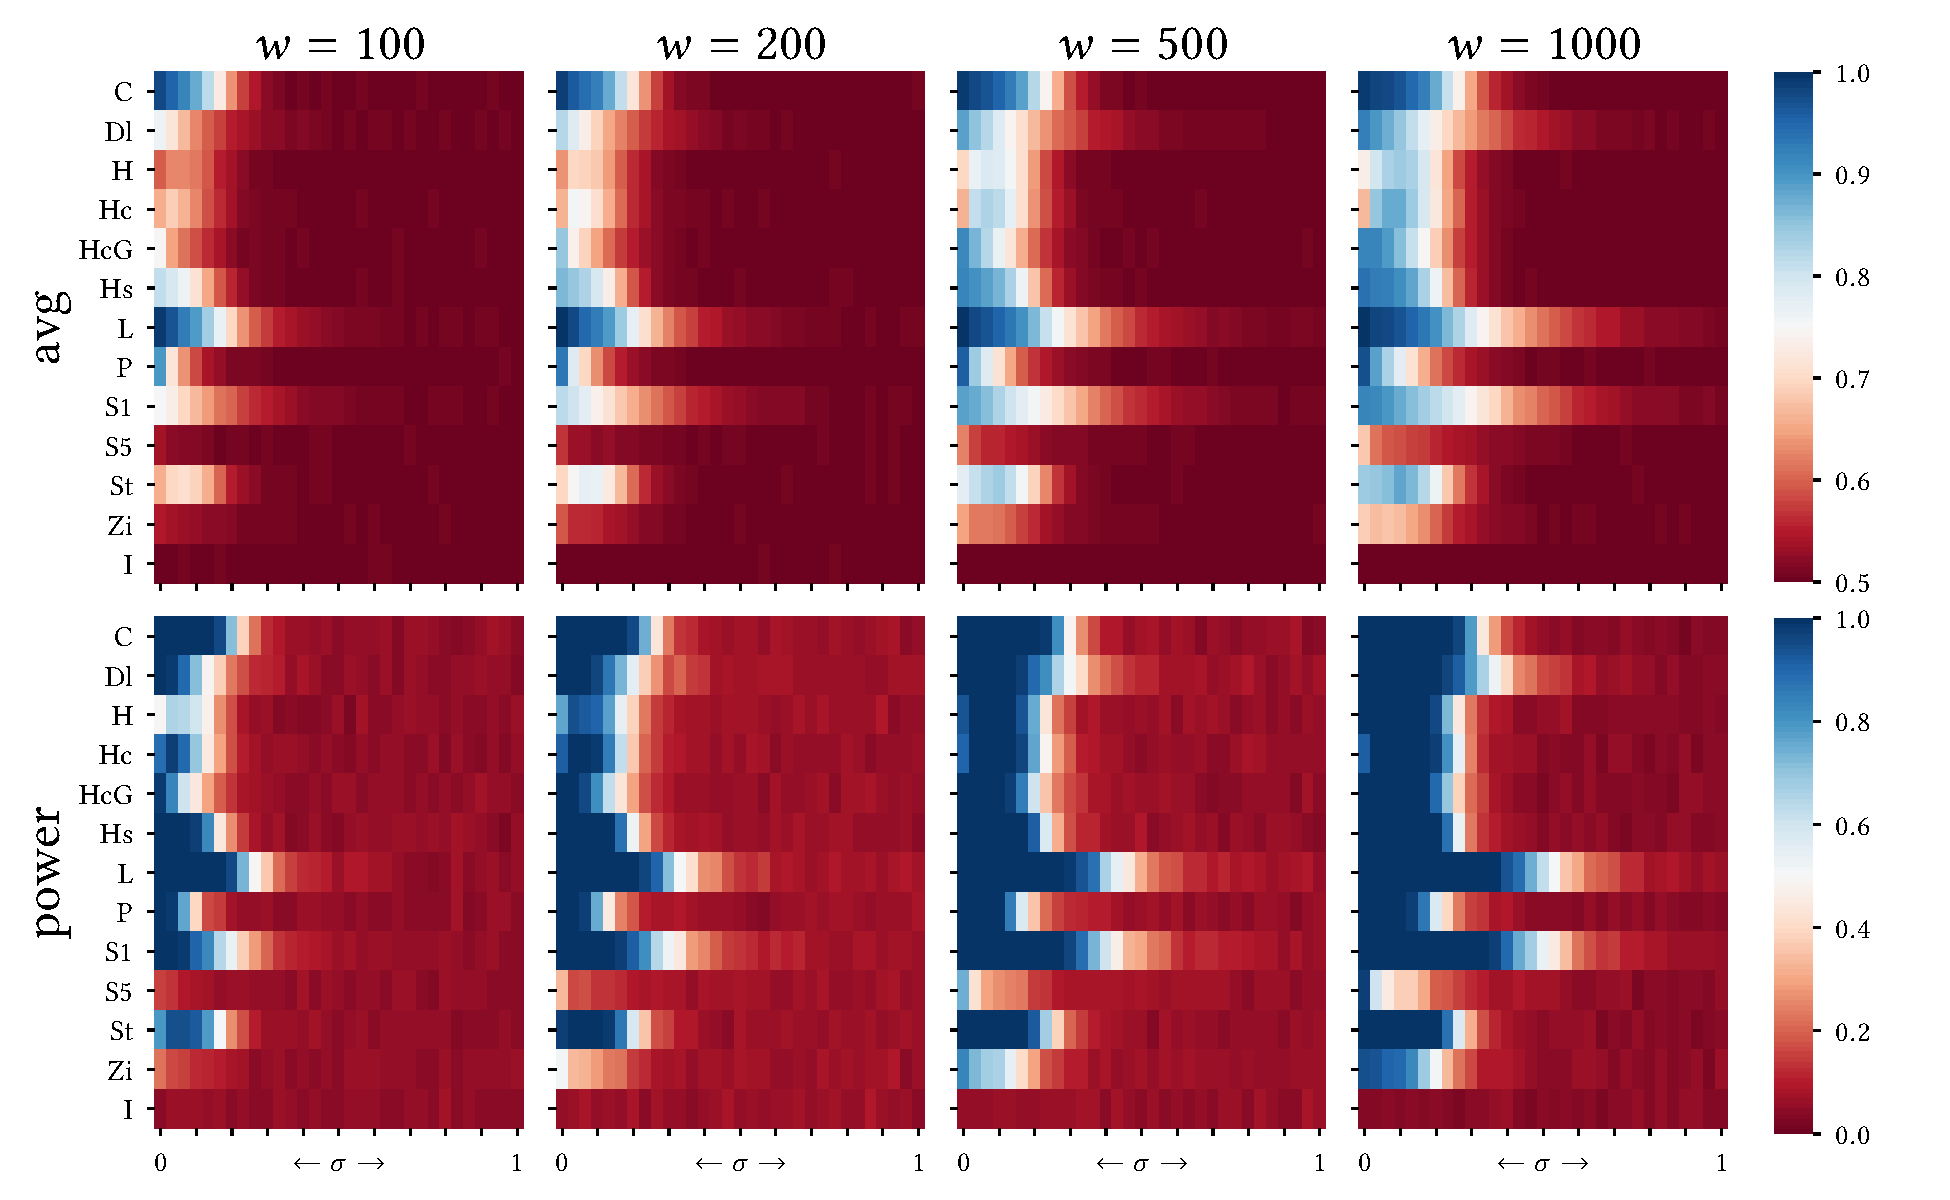
\includegraphics[width=\linewidth, trim=0 0.5cm 0 0.5cm]{part2-figures/Fig5_1-2_thesis-compressed.pdf}
	\caption{Power of \gls{MWP} w.r.t. $\gls{w}$.}
	\label{fig:N_MWP}
\end{figure}

\begin{figure}[ht]
	\centering
	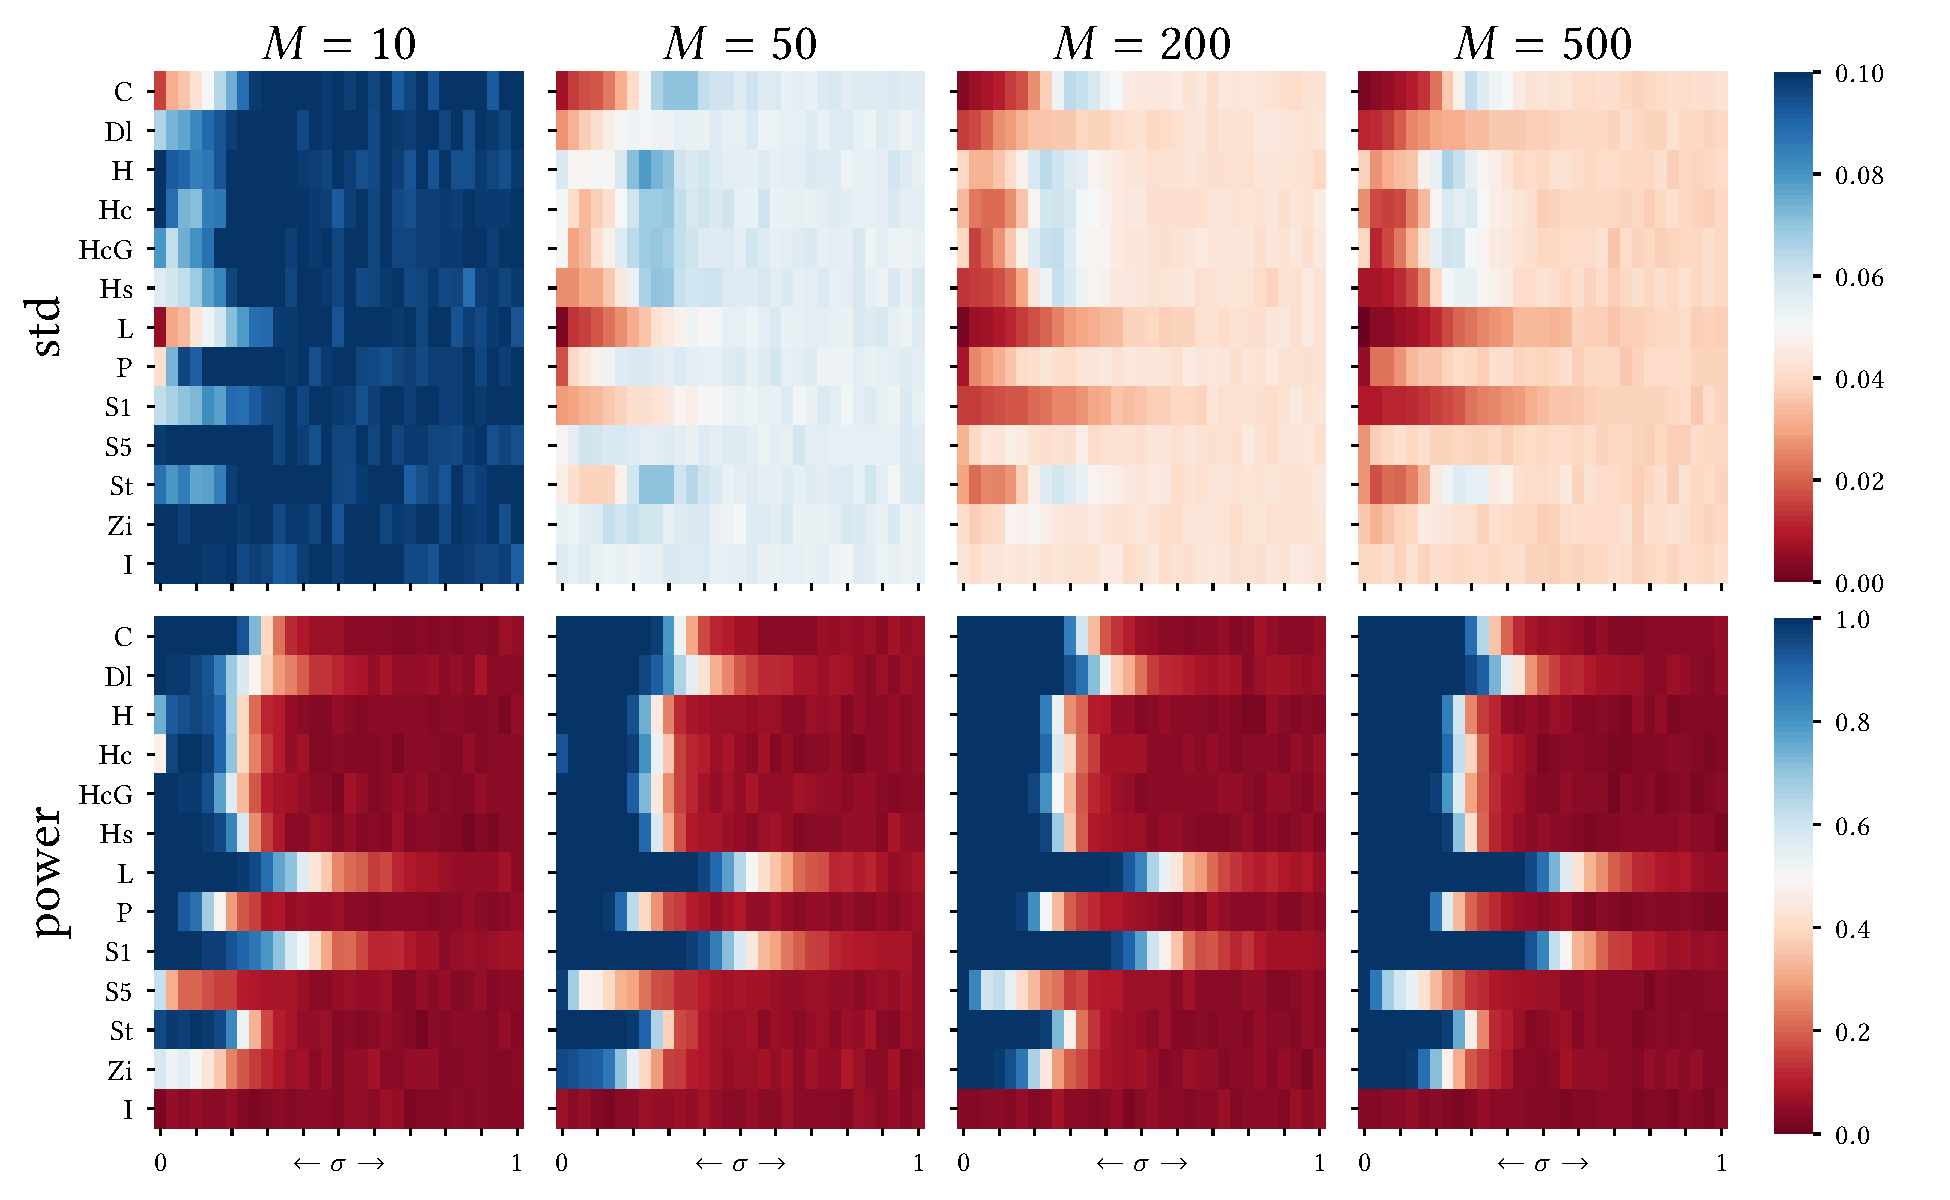
\includegraphics[width=\linewidth, trim=0 0.5cm 0 0.5cm]{part2-figures/Fig5_2-2_thesis-compressed.pdf}
	\caption{Power of \gls{MWP} w.r.t. $M$.}
	\label{fig:M_MWP}
\end{figure}

Figure~\ref{fig:N_MWP} shows that power globally increases with $\gls{w}$, but it is still high for most dependencies with low $\gls{w}$, provided noise is moderate. 
As we can see, the average score of \gls{MWP} tends to increase with $\gls{w}$, which explains the gain in power. That is because \gls{MWP} is sensitive (\hyperlink{R6}{\textbf{R6}}), as we discuss in \mbox{Section \ref{sensitivity}}.
Similarly, Figure~\ref{fig:N_MWP} shows that power increases slightly as $M$ increases, but the effect is visible only for S5 and Zi. We can explain this increase of power easily by the fact that the standard deviation of \textit{\gls{MWP}} decreases, which is what Theorem \ref{"th:hoeffding-chernoff-contrast"} predicted: with more iterations, the values concentrate around $\mathcal{C}$. 
In the end, we see that \gls{MWP} is already useful for small $\gls{w}$ or small $M$, even though more iterations or more data samples yield higher power when data is noisy. 

\begin{figure}
	\centering
	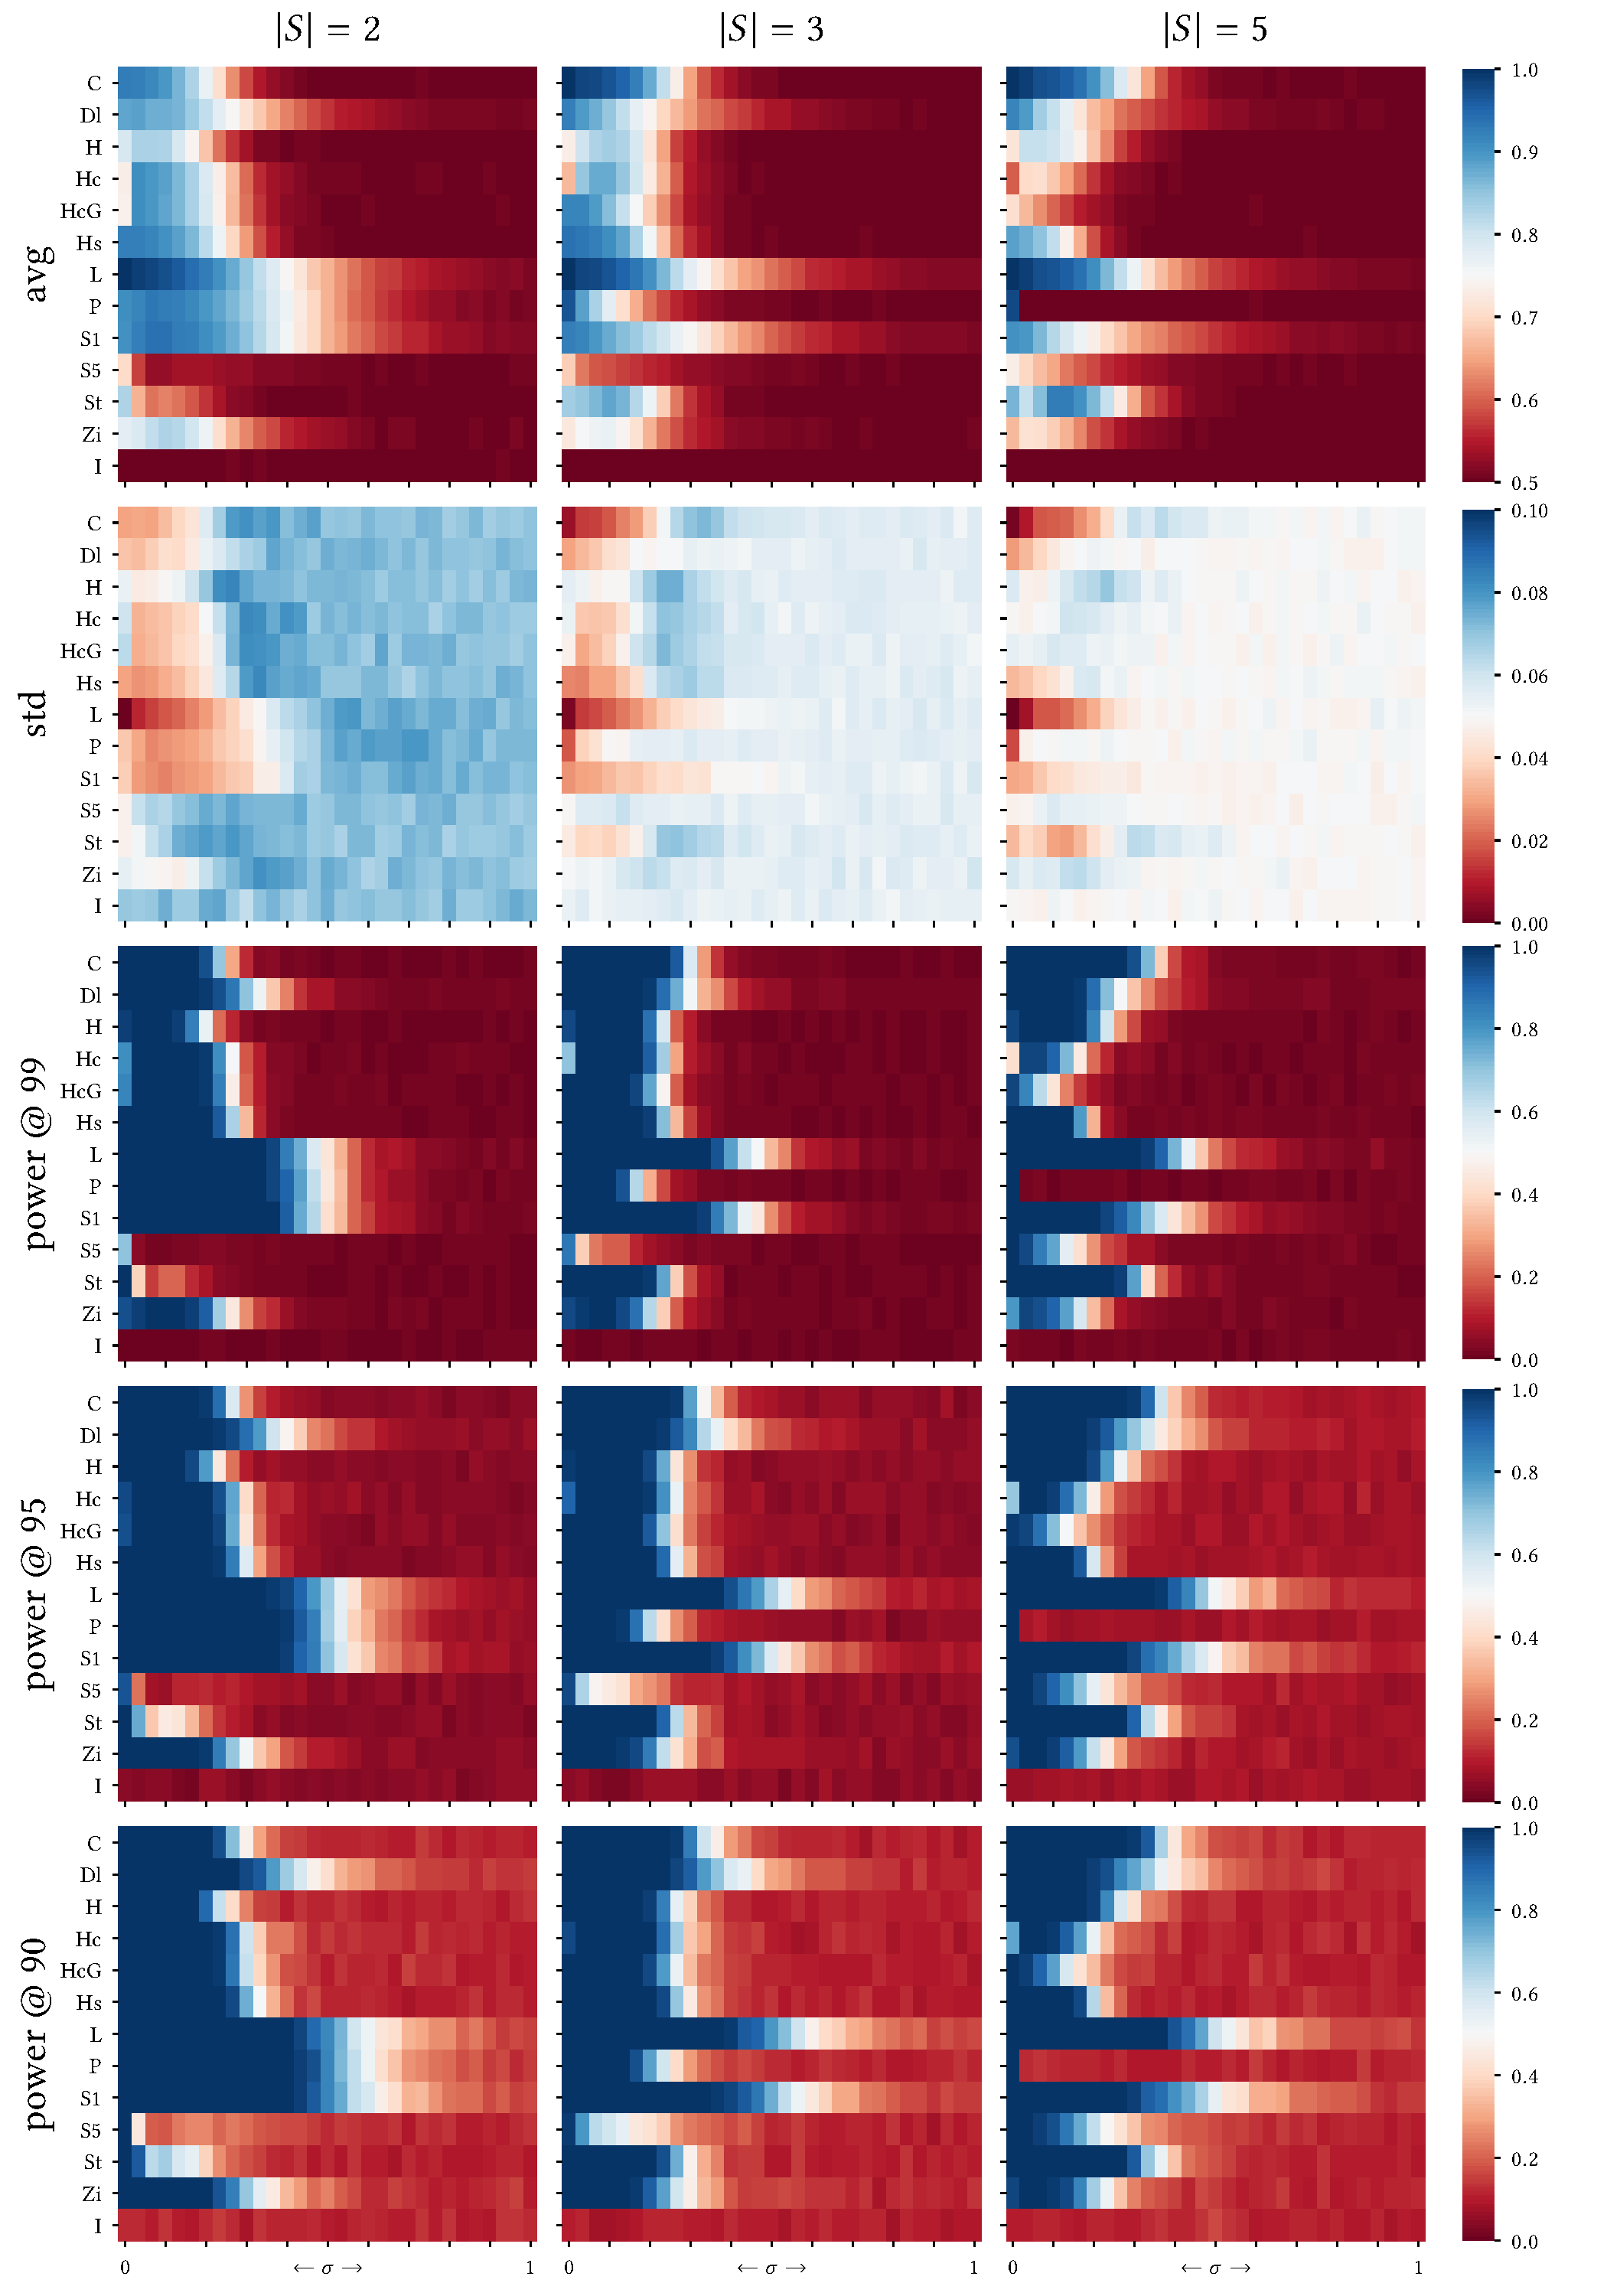
\includegraphics[width=1.0\linewidth]{part2-figures/Fig4-3_thesis-compressed.pdf}
	\caption{\gls{MWP} w.r.t. dimensionality $|\gls{S}|$.}
	\label{fig:momentsMWP}
\end{figure}

Figure~\ref{fig:momentsMWP} graphs the evolution of \gls{MWP} for $|\gls{S}| = 2,3,5$. 
As we see, the average \gls{MWP} decreases gradually for each dependency. The same level of noise does not seem to affect each estimate equally, also regarding dimensionality. 
For instance, the estimates of L, P and S1 are larger at $|\gls{S}|=2$.
While the estimates of Hc, HcG, P and Zi decrease with increasing $|\gls{S}|$, they increase for C and St. While some dependencies (e.g., Hc, HcG) appear to have lower contrast without noise, we see that this effect is not as visible when we decrease the threshold for measuring power. 
The standard deviation of \gls{MWP} increases with noise and decreases with $|\gls{S}|$. In particular, L, C and Hs have a low standard deviation. This means that fewer iterations are required to estimate stronger dependencies. 
Power does not seem to vary much with dimensionality for most dependencies. It decreases with $|\gls{S}|$ for Hc, HcG, Hs, P and Zi, while it increases for C, S5 and St. 

All in all, each dependency yields a score larger than I up to a certain level of noise, leading to high power. Thus, \gls{MWP}, and, by extension, \gls{MCDE}, are general-purpose (\hyperlink{R2}{\textbf{R2}}).

\subsubsection{Comparison to Competing Approaches}

\begin{figure*}
	\centering
	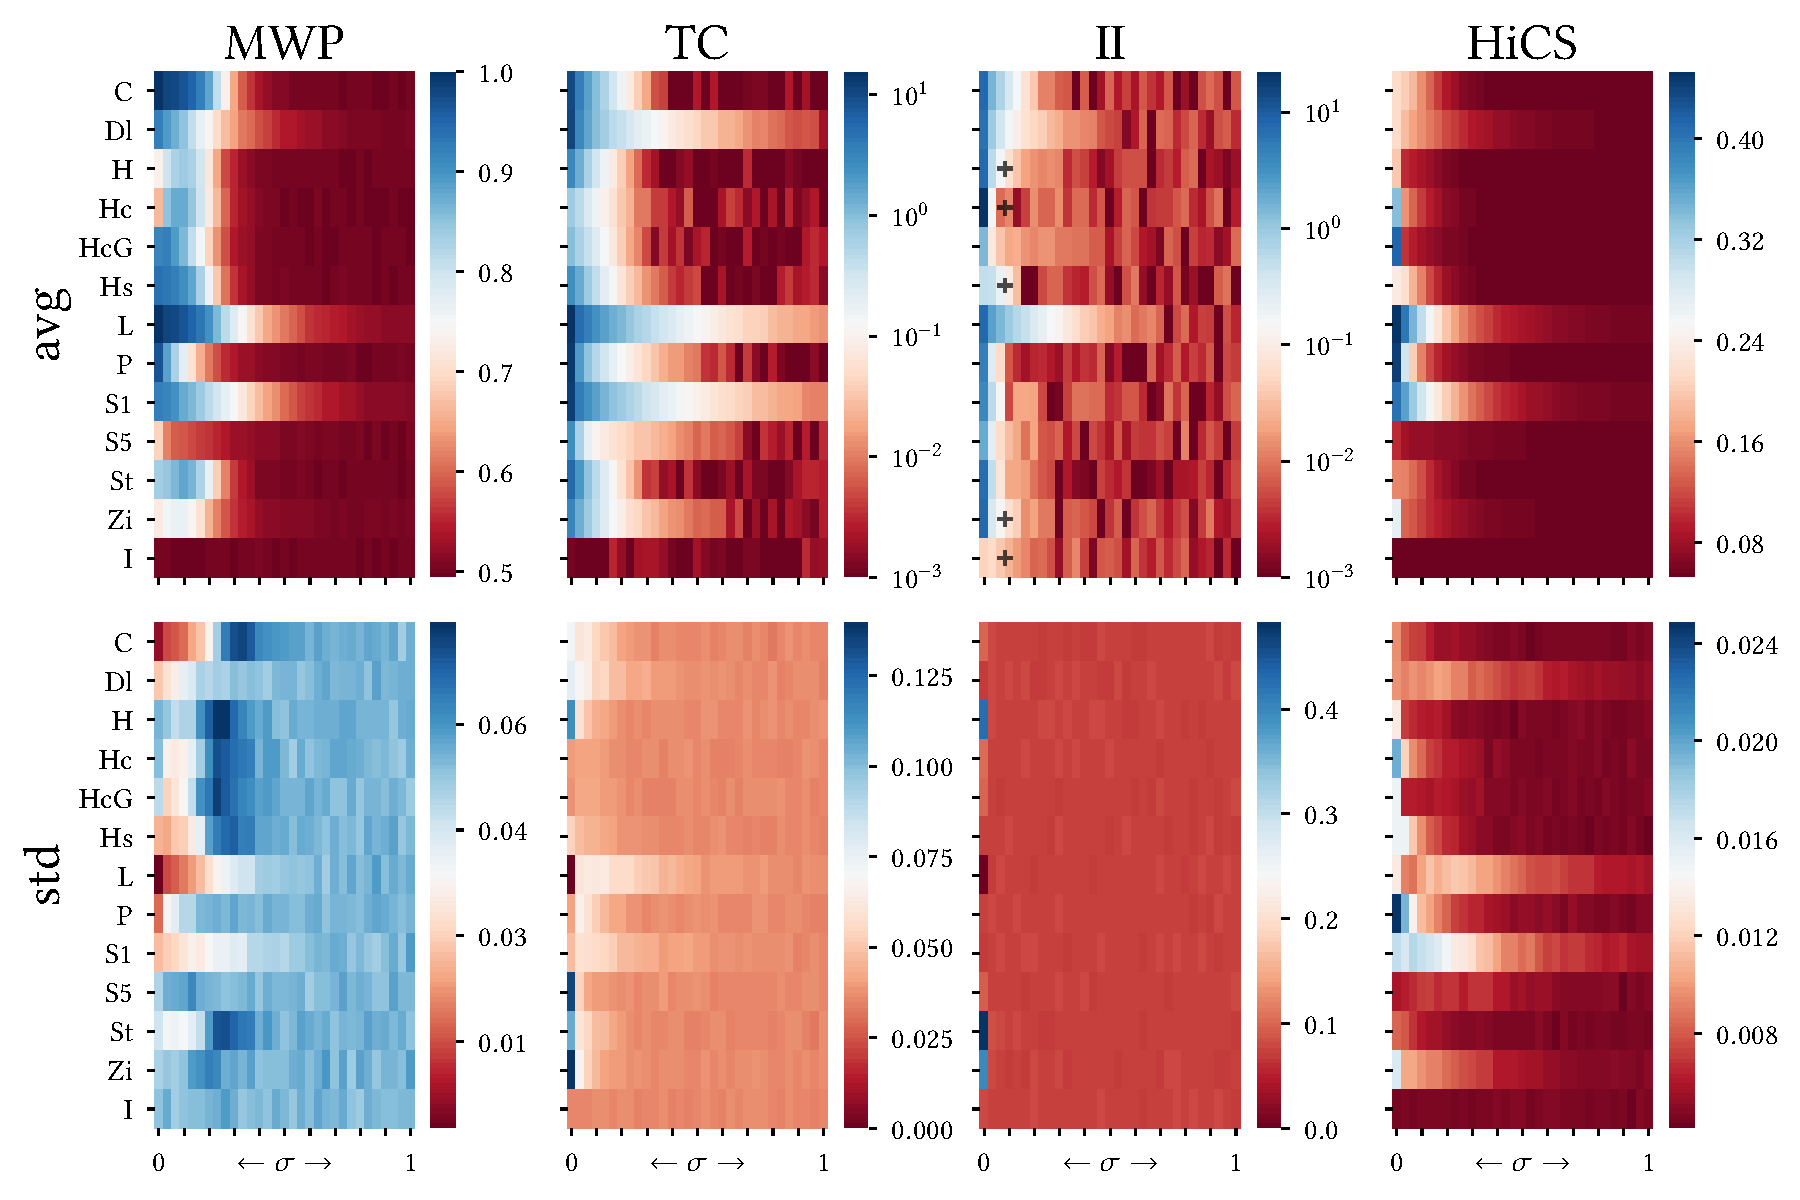
\includegraphics[width=1.0\linewidth]{part2-figures/Fig6_large_1-2_thesis-compressed.pdf}
	\hfill
	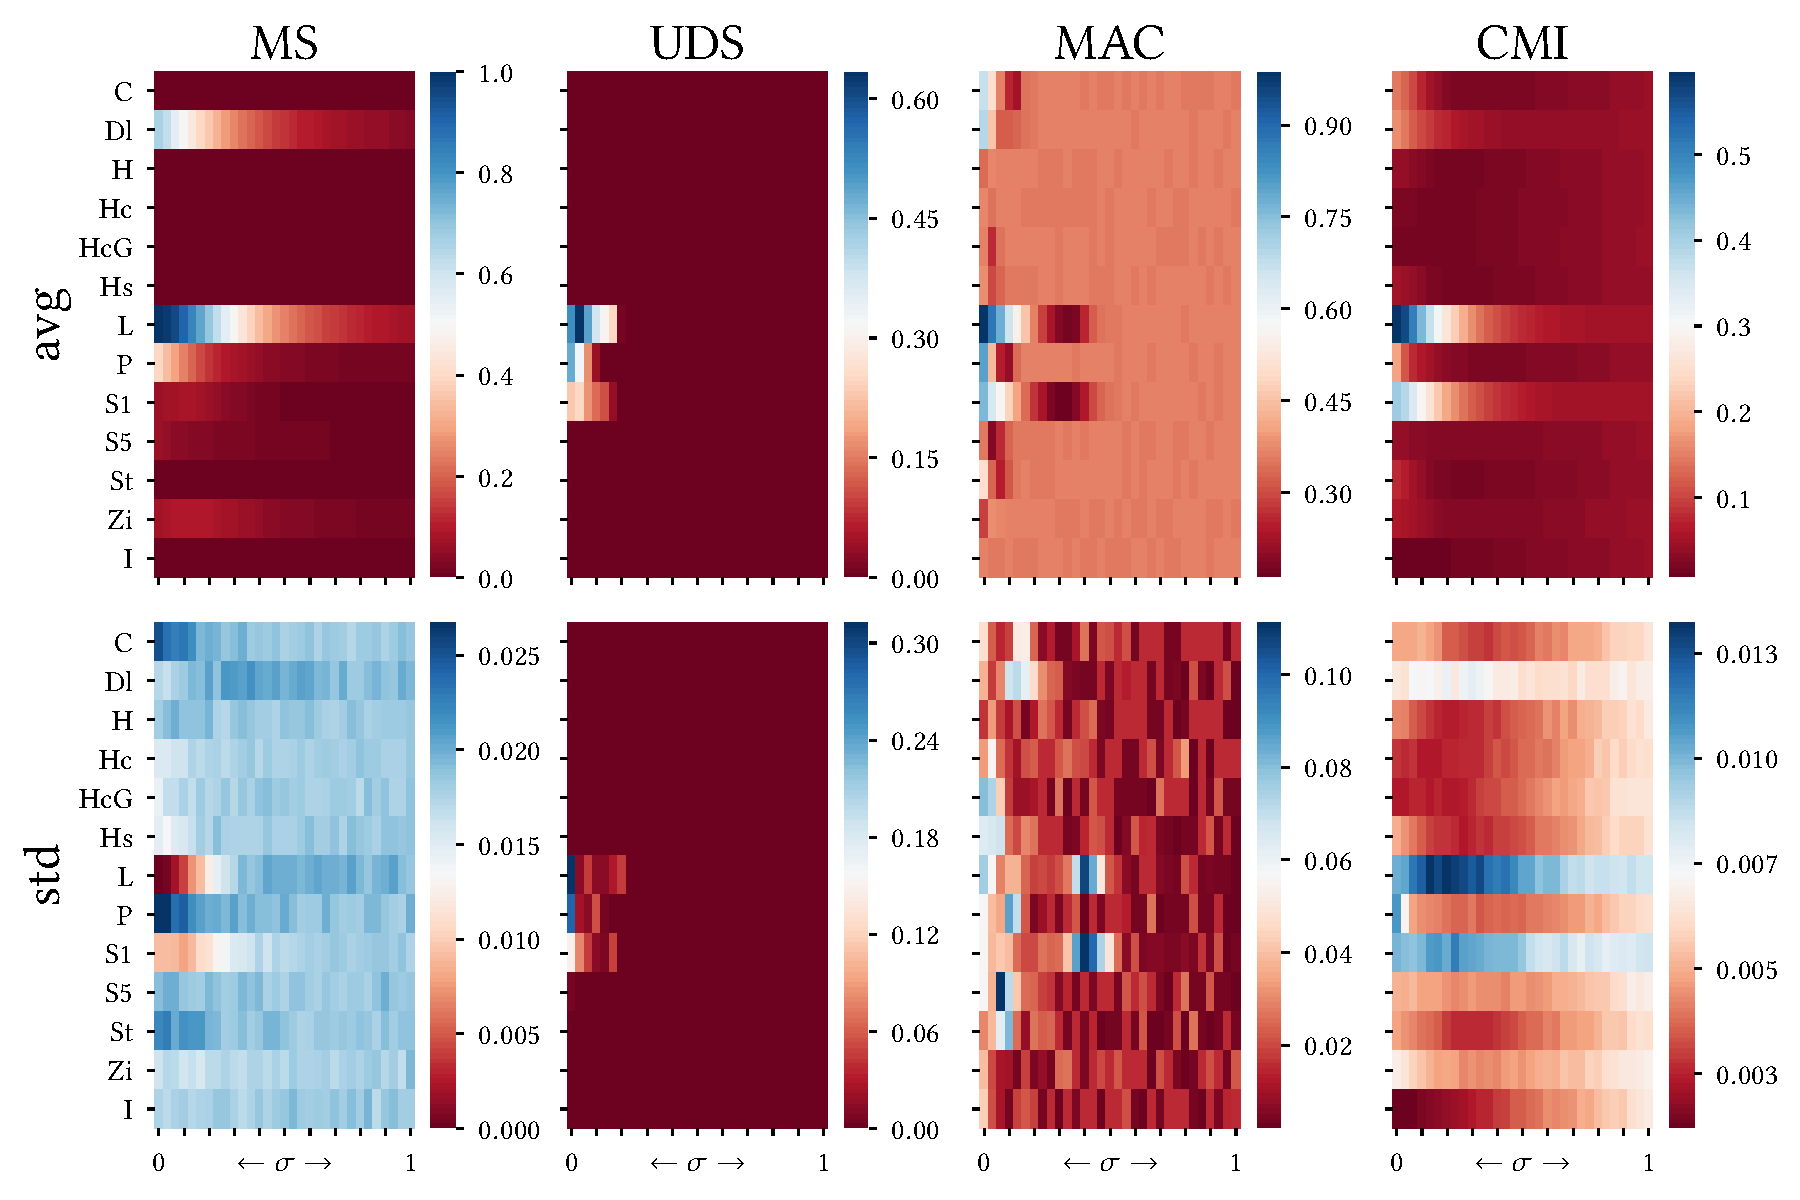
\includegraphics[width=1.0\linewidth]{part2-figures/Fig6_large_2-2_thesis-compressed.pdf}
	\caption{Distribution of dependency estimation scores, $|\gls{S}|=3$.}
	\label{fig:contrast_all}
\end{figure*} 

We compare the score distribution for each competing approach with \gls{MWP} in Figure~\ref{fig:contrast_all}. First, we see that the average score of \gls{MWP} is most similar to \gls{TC}. However, \gls{TC} is unbounded, and its scores follow a logarithmic scale. This means that the estimates of \gls{TC} change very abruptly. We see that \gls{MWP} scores are slightly smaller for noiseless dependencies with many ties w.r.t. marginal distributions, such as H and Hc, which we attribute to the correction for ties in the Mann-Whitney U test.
 
\gls{II} can yield positive or negative values. %Since both cases are interesting, 
We visualise the absolute value of \gls{II} with a logarithmic scale. We mark the dependencies which obtain a positive score in their noiseless form with a plus sign.
\gls{II} assigns high scores to every noiseless dependency. However, the score decreases rapidly with noise, except for L.

\gls{HiCS} shows a similar behaviour as \gls{MWP}, except that the scores decrease faster, and that many dependencies start with a relatively 
low score, even in the noiseless form, such as C, Dl, H,  Hs, S5 and St. 
Next, \gls{MS} and \gls{UDS} are restricted to monotonous and bijective functional relationships, respectively. They can detect only 3 out of 12 dependencies. \gls{MAC} and \gls{CMI} behave curiously. Their scores change noticeably only for C, Dl, L, P and S1.
The values of \gls{MAC} also change abruptly and even non-monotonously with noise. For example, L and S1 obtain lower scores with a noise level of 0.3 than with higher noise levels. 
\gls{CMI} evolves smoothly. However, for many dependencies, including I, the score increases again with more noise: the shades on the right are lighter, which shows a bias towards noise, independently of the underlying relationship.

By looking at \gls{MWP} and \gls{MS}, we see that the standard deviation behaves similarly: it decreases as the score increases. We observe the opposite for \gls{HiCS}. The standard deviation of \gls{CMI} reaches its highest level at a certain noise level, around $0.2$ for \gls{L}, and tends to increase slightly again with more noise. %For \gls{UDS} and \gls{MAC}, the evolution of the standard deviation looks very unstable. The standard deviation of \gls{TC} and \gls{II} does not change much, except for noiseless dependencies.

While \gls{HiCS}, \gls{UDS}, \gls{MAC} and \gls{CMI} are expected to be in $[0,1]$, the theoretical maximum or minimum is never reached, even if our benchmark features both strong and weak dependencies. On the other hand, \gls{MWP} and \gls{MS} exploit all the values of their range, being $[0.5,1]$ and $[0,1]$ respectively. Thus, they are interpretable (\hyperlink{R6}{\textbf{R6}}).

\begin{figure}
	\centering
\begin{subfigure}[$|\gls{S}|=3$]
	{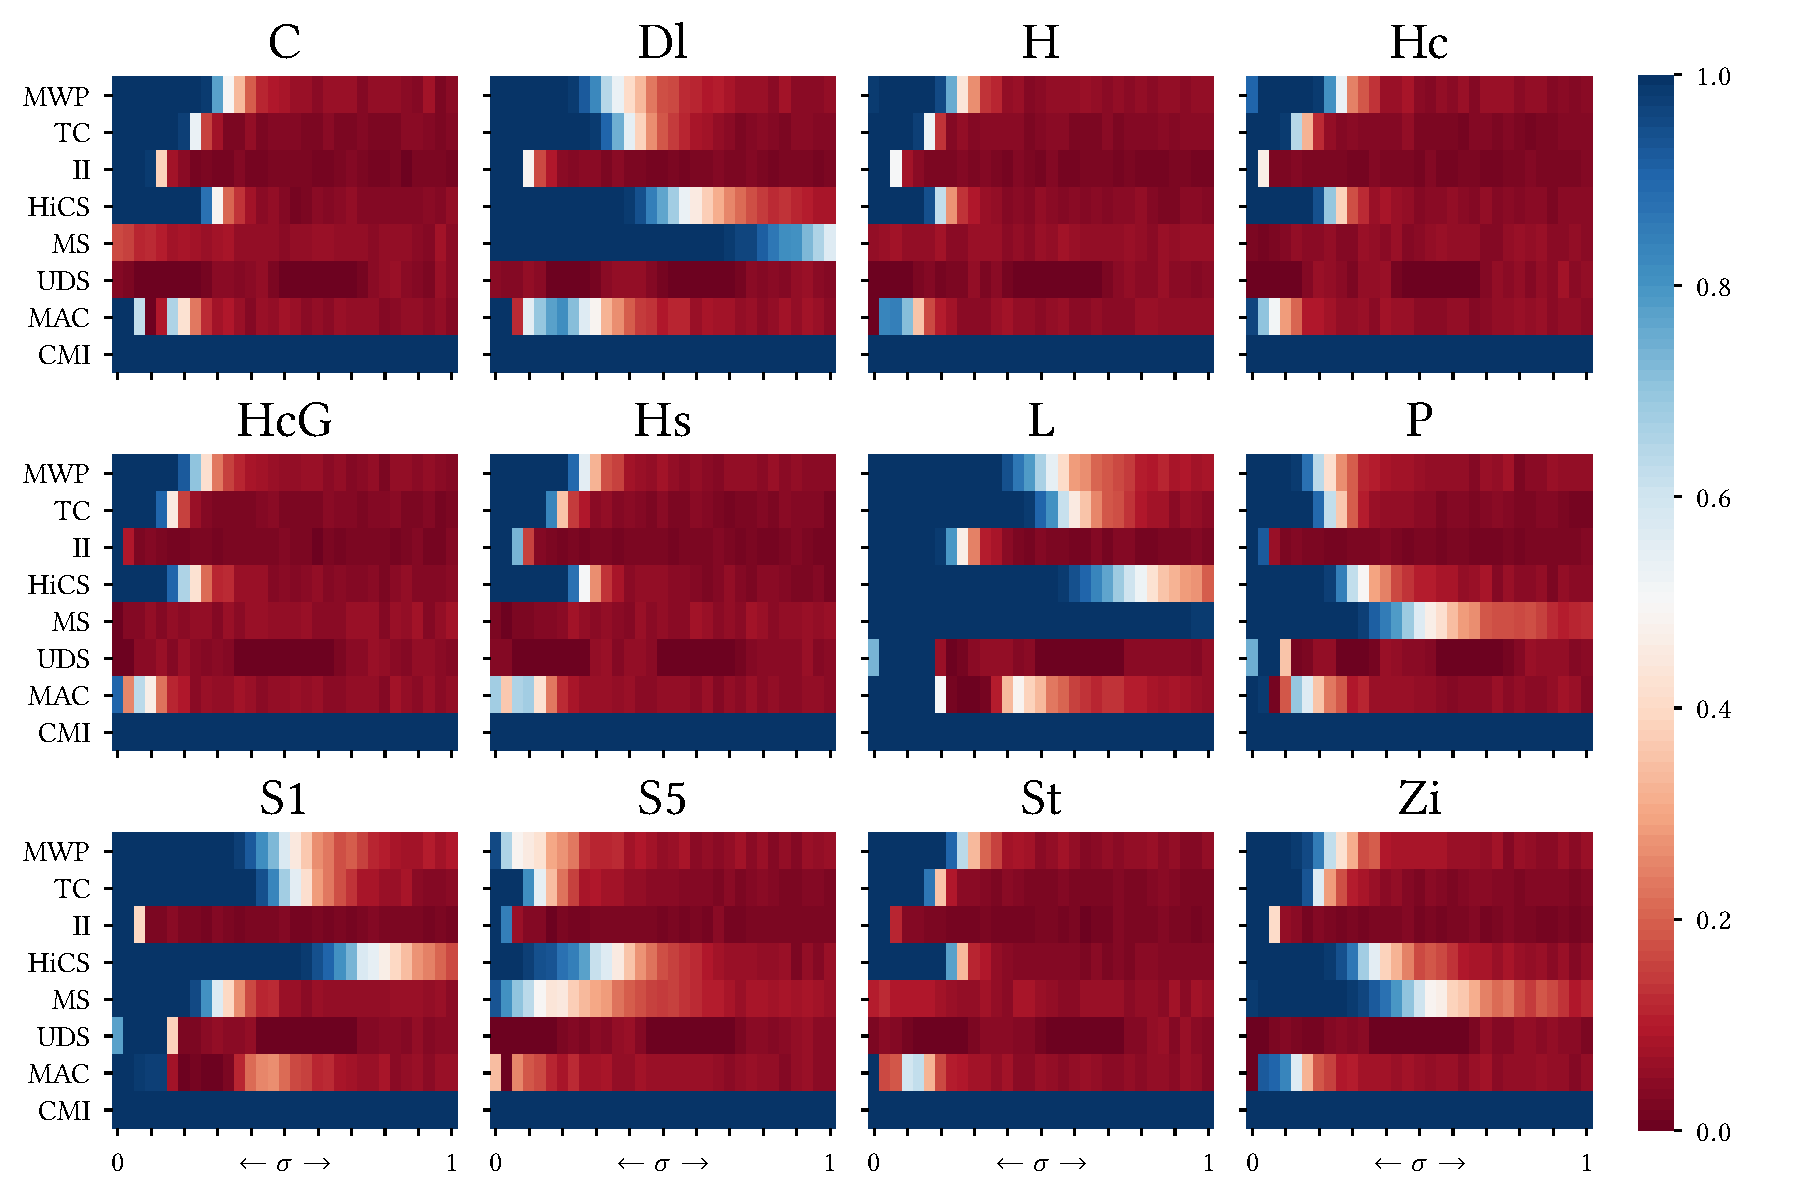
\includegraphics[width=1.0\linewidth]{part2-figures/Fig7_d3-2_thesis-compressed.pdf}}
\end{subfigure}
\begin{subfigure}[$|\gls{S}|=5$]
	{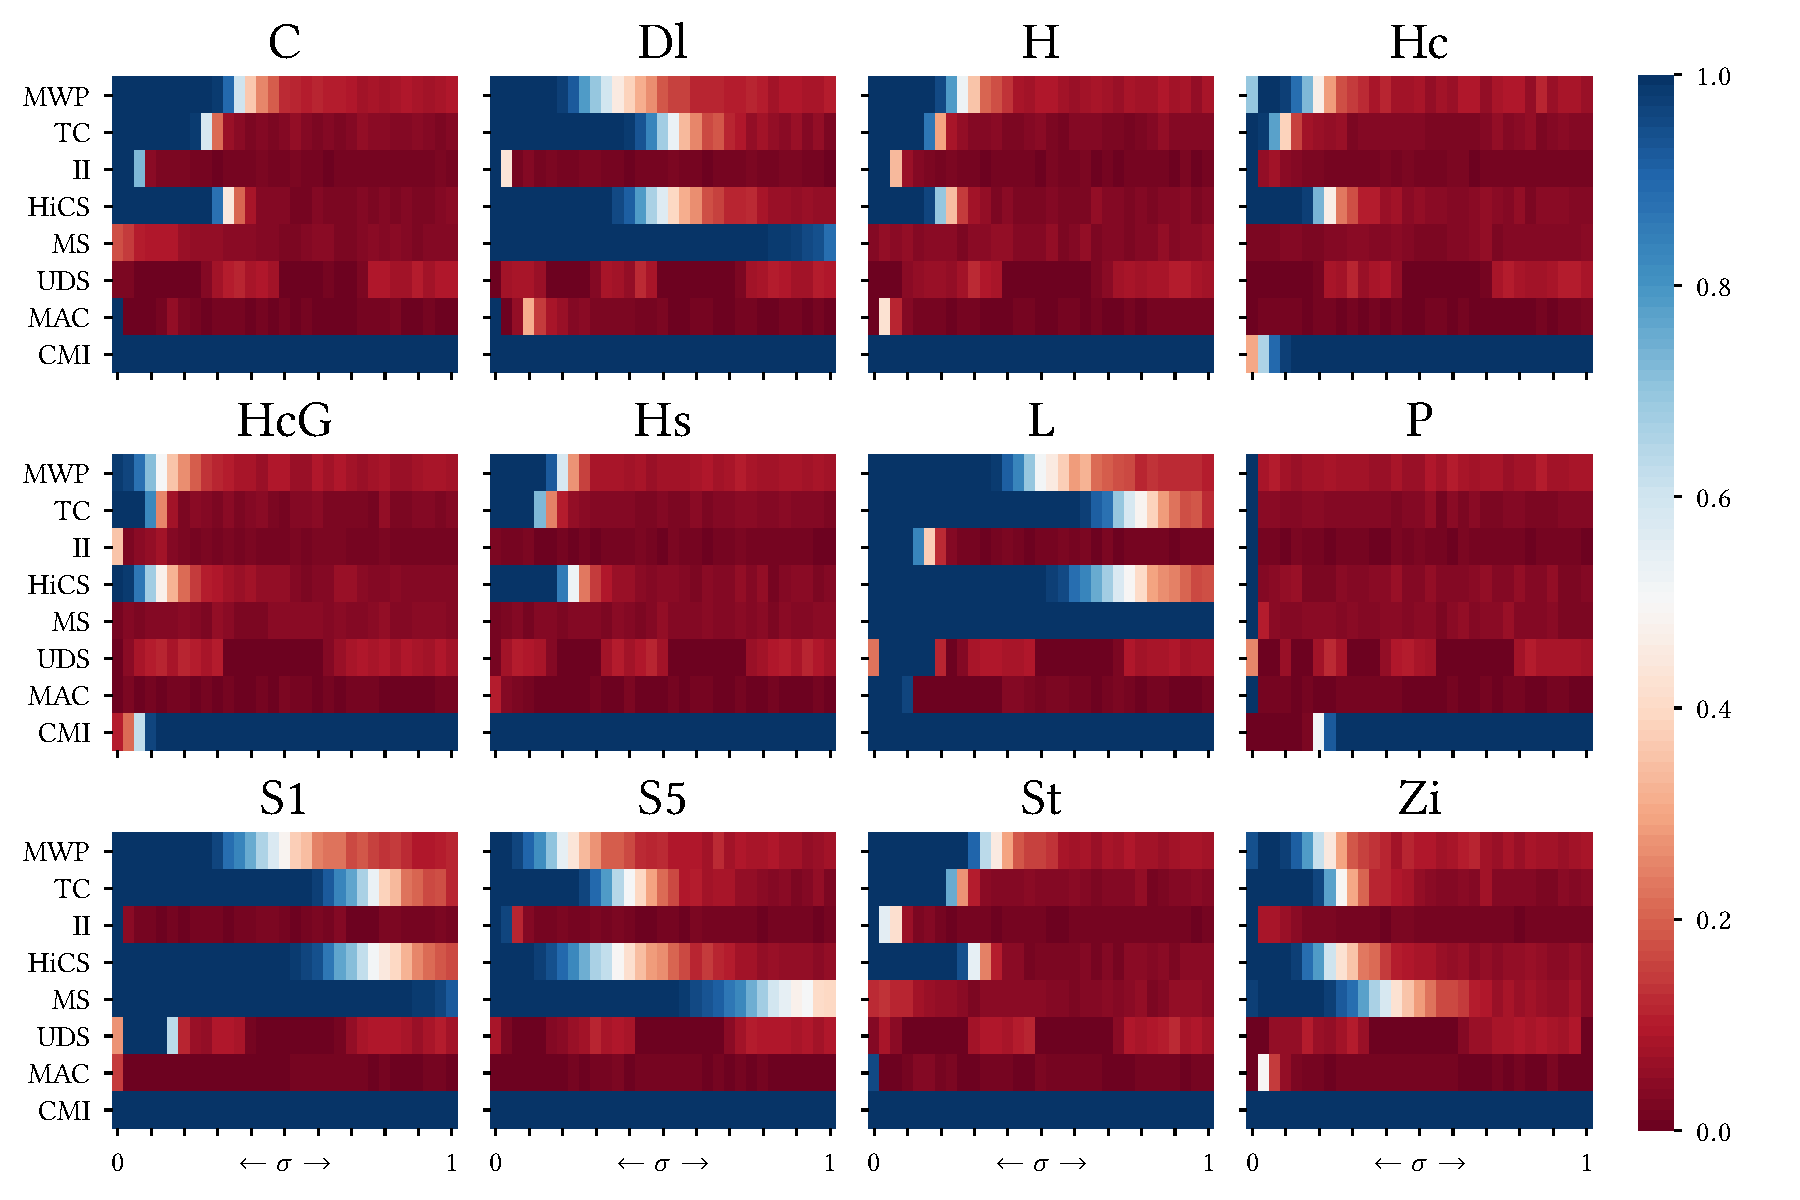
\includegraphics[width=1.0\linewidth]{part2-figures/Fig7_d5-2_thesis-compressed.pdf}}
\end{subfigure}
\caption{Power against each dependency.}
\label{fig:E_Power}
\end{figure}

Figure \ref{fig:E_Power} reveals that \gls{MWP}, \gls{TC} and \gls{HiCS} achieve high power in any situation up to a certain extent of noise. 
\gls{MWP} shows slightly more power with C, H, Hc, HcG, Hs and St.  
\gls{II} can detect almost every dependency, but the power decreases rapidly with noise and dimensionality. \gls{MS} detects Dl, L, P, S1, S5 and Zi, but misses all other dependencies. 
\gls{MAC} looks unstable since its power evolves in a non-monotonous way and decreases with increasing dimensionality by much. In fact, it is not able to detect most dependencies for $|\gls{S}|=5$.  
\gls{UDS} can only detect L, P and S1, a clear limitation. 
\gls{CMI} has maximal power for each dependency and noise level for $|\gls{S}|=3$, which is unrealistic: \gls{CMI} reaches its lowest score against the noiseless I, our baseline for power. This means that \gls{CMI} does not clearly distinguish noise from dependence. 

\subsubsection{Sensitivity}
\label{sensitivity}

\hyperlink{R6}{\textbf{R6}} states that estimators should reflect the strength of the observed effect w.r.t. the number of observations. Figure \ref{fig:All_sensitivity} graphs the average score from 500 instances of each dependency with a minimal noise of $1/30$. The average of \gls{MWP} obtained for each dependency converges to 1 consistently with more samples, except for I, which stabilises around $0.5$. This means that \gls{MWP} is sensitive (\hyperlink{R6}{\textbf{R6}}). 

\gls{TC} behaves similarly to \gls{MWP}. %: When the sample size increases, the score tends to increase as well. 
However, it is not bounded. While the scores of \gls{II} seem to increase with sample size, their absolute value decreases. %, except for \textbf{Hs}. 
\gls{MS} is %completely 
insensitive to changes in sample size. \gls{HiCS}, \gls{UDS}, \gls{MAC} and \gls{CMI} behave differently: their scores tend to go down as the sample size increases, even with I. This implies that their minimum or maximum score varies with the sample size, also highlighting interpretability (\hyperlink{R5}{\textbf{R5}})  problems. 

\begin{figure}
	\centering
	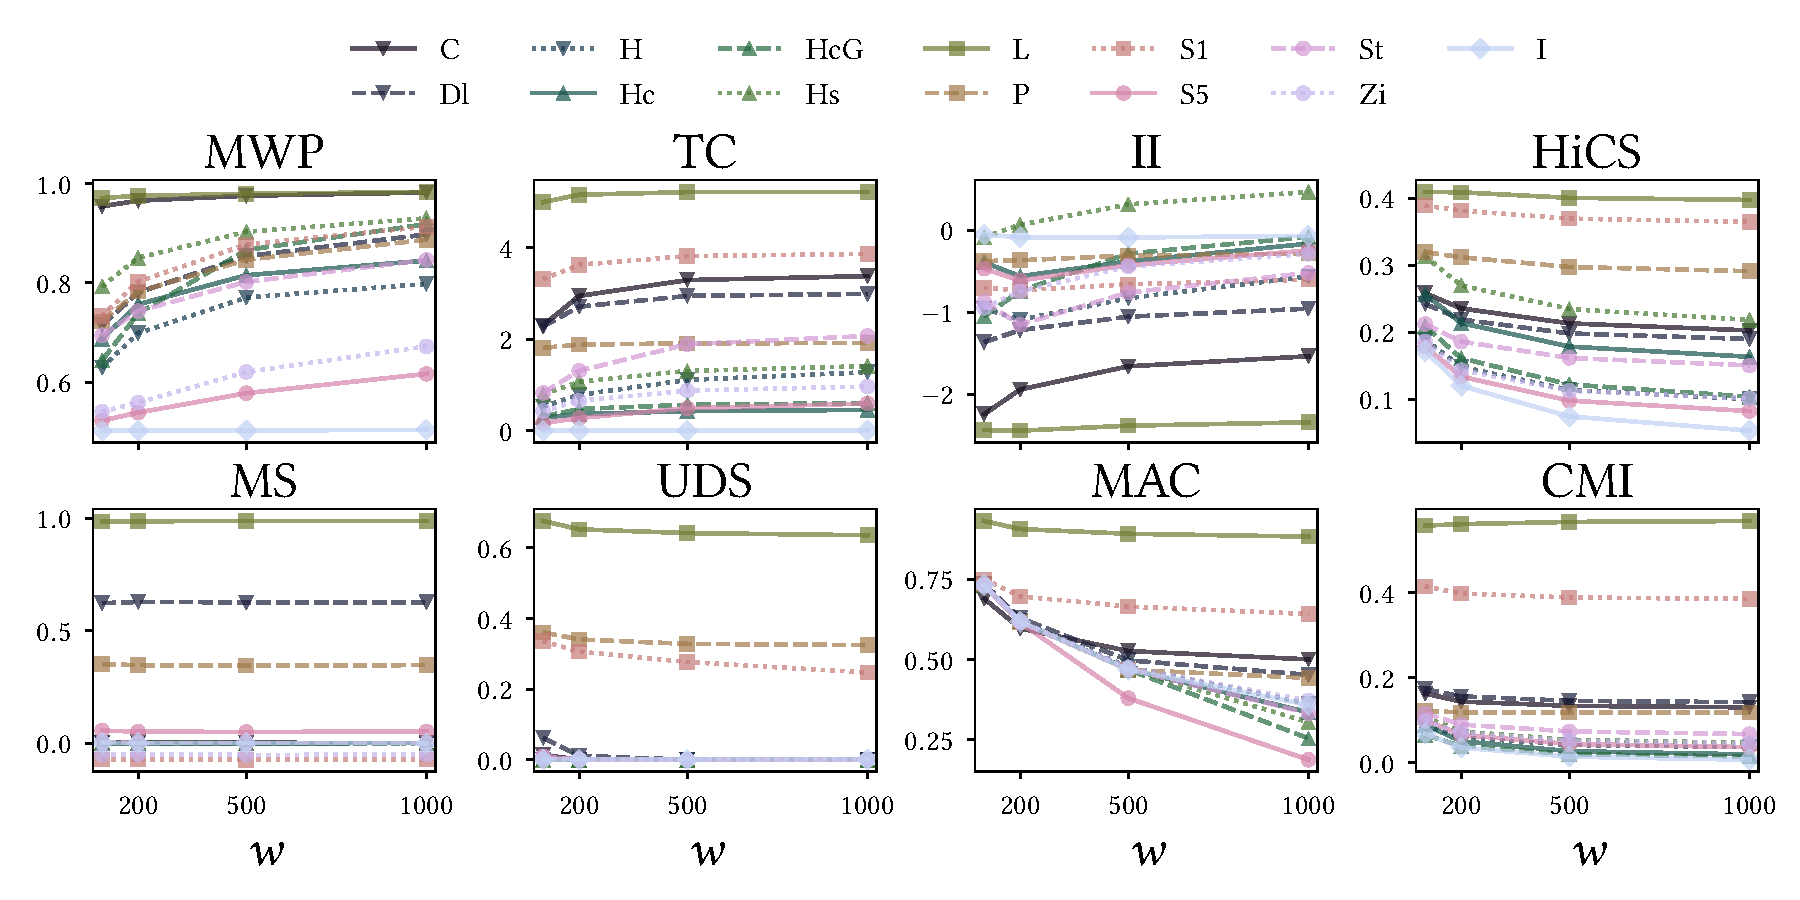
\includegraphics[width=\linewidth]{part2-figures/Fig8-2_thesis-compressed.pdf} 
	\caption{Average score w.r.t. $\gls{w}$, $\sigma = 1/30$.}
	\label{fig:All_sensitivity}
\end{figure} 

\subsubsection{Robustness}
\label{robustness}

\begin{figure}
	\centering
	\begin{subfigure}[Power]
		{\label{fig:E_Discrete_Power}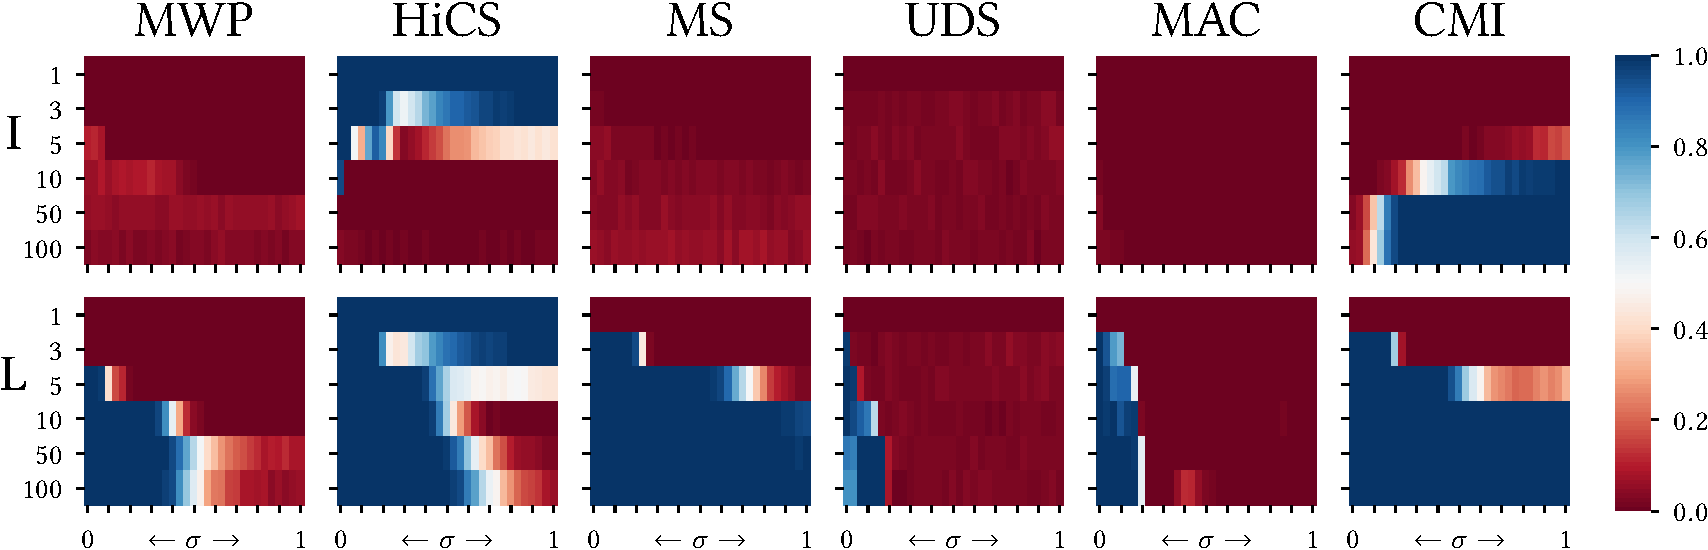
\includegraphics[width=\linewidth]{part2-figures/Fig9_1_thesis-crop-compressed.pdf} }
	\end{subfigure}
	\begin{subfigure}[Average]
		{\label{fig:E_Discrete_average}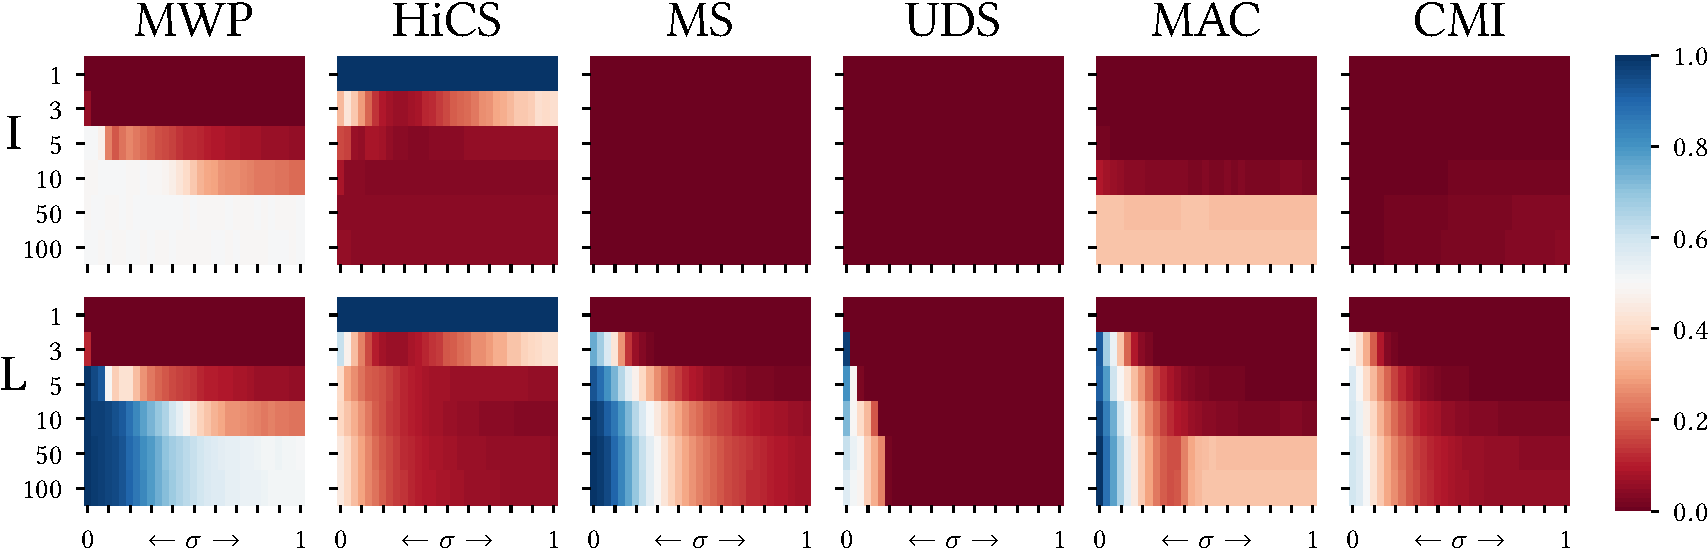
\includegraphics[width=\linewidth]{part2-figures/Fig9_2_thesis-crop-compressed.pdf}  }
	\end{subfigure}
	\caption{Power and average score w.r.t. $\omega$.}
	\label{fig:E_Discrete}
\end{figure} 

Data is often imperfect, i.e., values are rounded or trimmed. In some cases, this may lead to wrong estimates, e.g., an independent space is declared as strongly dependent. 

We simulate data imperfections by discretising a 3-dimensional linear dependency into a number $\omega$ of discrete values from 100 to 1. With only one value, the space is entirely redundant, i.e., its \textit{contrast} should be minimal. We compare the power of \gls{MWP} and the other approaches against L and I for different levels of discretisation. Since \gls{TC} and \gls{II} base on local neighbourhoods, they do not work in this setting%they fail when the same observation is present more than $k$ times, i.e., they are by design not robust
; We exclude them from the analysis. Figure \ref{fig:E_Discrete_Power} displays the results.

\gls{HiCS} yields high power in the case of discrete values, even for I. %This is because \gls{HiCS} uses the \textit{Kolmogorov-Smirnov} test which assumes continuous data. 
Thus, \gls{HiCS} is not robust. Also, the power of \gls{CMI} wrongly increases as we add noise to I, provided that $\omega \geq 10$. 
This is why the power of \gls{CMI} is high for every dependency in Figure \ref{fig:E_Power}. \gls{CMI} rejects the independence for independent spaces, i.e., it is not robust. On the other hand, \gls{MWP}, \gls{MS}, \gls{UDS} and \gls{MAC} seem robust (\hyperlink{R7}{\textbf{R7}}).

In Figure \ref{fig:E_Discrete_average}, we see that the score of \gls{CMI} tends to increase slightly for I as we add noise, whenever $\omega > 5$. Also, the score of \gls{HiCS} increases for both I and L when $\omega \leq 5$. \gls{MAC} converges to $0.4$ as noise increases for $\omega > 10$. On the other hand, \gls{MWP} converges to $0$ as the space becomes discrete. This is an interesting feature of our estimator: discrete spaces are of lower interest since the notion of \textit{contrast} is not clearly defined there. It allows analysts to draw a line between discrete and real-valued attributes, characterizing their relevance for further analysis.   

\subsubsection{Scalability}
\label{sec:scalability}

\begin{figure}
	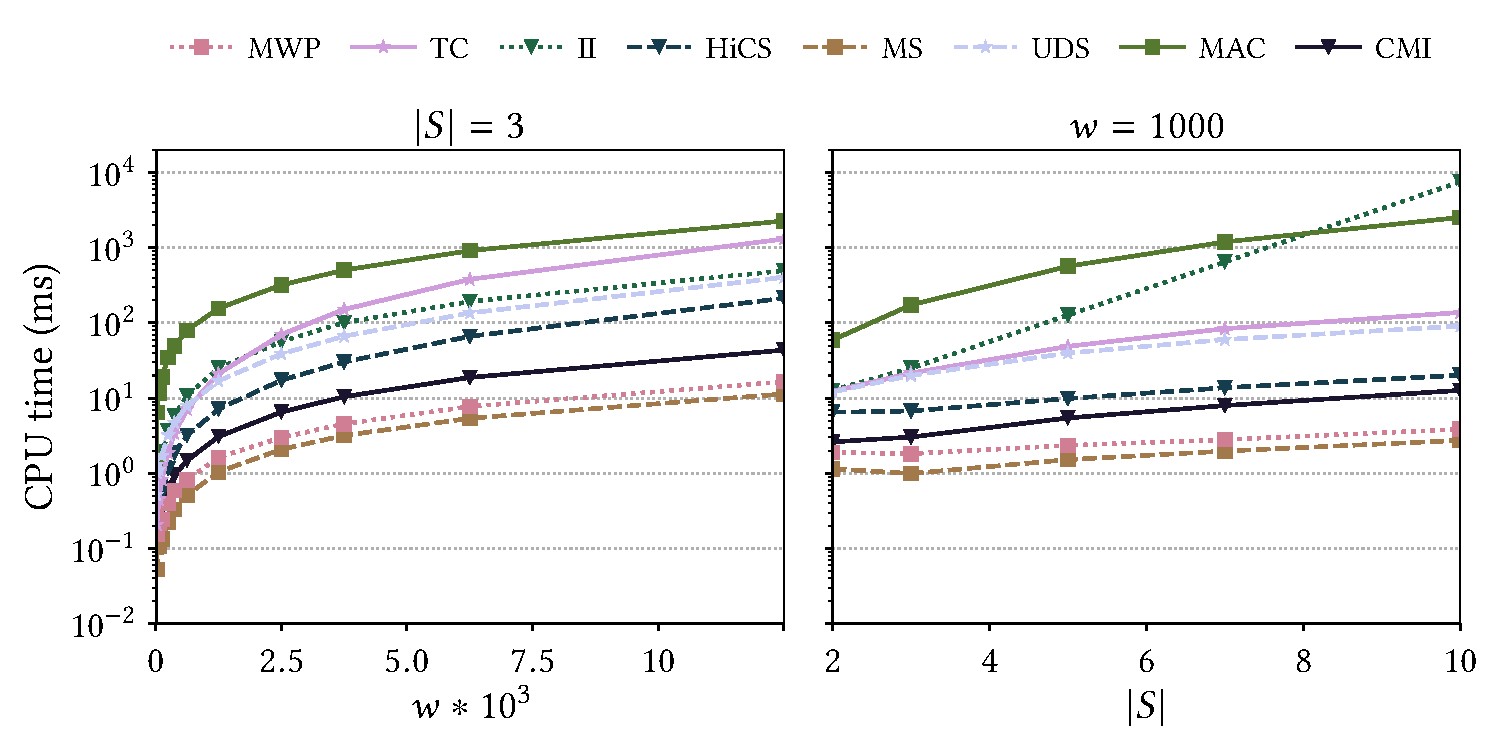
\includegraphics[width=1.0\linewidth]{part2-figures/Fig10-2_thesis-compressed.pdf} 
	\caption{Execution time w.r.t. $\gls{w}$ and $|\gls{S}|$.}
	\label{fig:Runtime_n_d}
\end{figure} 

We now look at the runtime requirements of our approach. We measure the average time for each estimator against $500$ independent data sets with growing $\gls{w}$ and $|\gls{S}|$. Note that which data set we use only has a marginal effect on the measured time. For consistency, we use instantiations of I for every estimator. 
Figure \ref{fig:Runtime_n_d} graphs the results. As we can see, \gls{MWP} is the second fastest after \gls{MS}. 
\gls{HiCS} and \gls{CMI} scale relatively well with $\gls{w}$ and $|\gls{S}|$. There is a second group formed by \gls{TC}, \gls{II} and \gls{UDS} one order of magnitude slower. However, \gls{II} does not scale well with $|\gls{S}|$. \gls{MAC} is way behind all others. One should note that the runtime of \gls{MWP} can be further improved via parallelisation and prior indexing.

We evaluate the scalability of index construction for each approach, by increasing the size of the sliding window $\gls{w}$ from $10^2$ to $10^5$ in an independent space I with three dimensions. 
The red line (`Construction') is the average time for creating the index with window size $\gls{w}$ (Algorithms \ref{indexconstruction}/\ref{kspconstructindex}/\ref{cspconstructindex}). 
The other lines show the average time to insert a new point into the window.   
\begin{figure}
    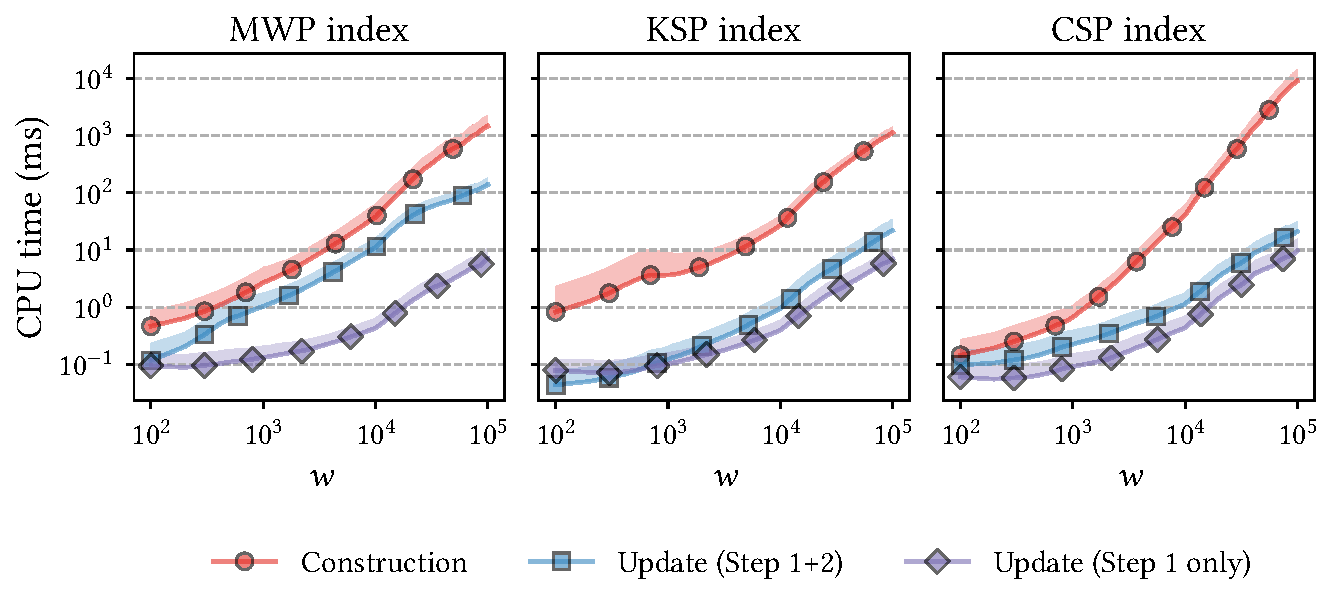
\includegraphics[width=\linewidth]{part2-figures/indexperformance_thesis-compressed.pdf}
    \caption{Time required for index construction and update w.r.t. window size $\gls{w}$.}
    \label{fig:scalability-index}
\end{figure}

In Figure \ref{fig:scalability-index}, we can see that the construction time of each index increases almost linearly with increasing window size $\gls{w}$. 
The \gls{KSP} index is less expensive to update than \gls{MWP}, regarding \textsc{Step 2} in particular. 
The first step of the \gls{CSP} index update is very efficient, as it requires more or less constant time (see Table \ref{tab:complexity}). 
We can see that only performing \textsc{Step 1} in our update operations, while delaying \textsc{Step 2} to the contrast estimation step, reduces the execution time by up to 3 orders of magnitude, compared to standard index construction. 
So we can significantly speed up the monitoring of \gls{MCDE} contrast using the index update operations. 

In Figure \ref{fig:scalability-contrast}, we compare the execution time estimating \gls{MWP}, \gls{KSP}, and \gls{CSP}, with increasing window size $\gls{w}$. 
We can see that the three approaches have a comparable execution time. 
\gls{KSP} is slightly slower for small window sizes because the $\overline{p}$-values are more difficult to obtain than with the other approaches. 
However, as the window size increases, \gls{KSP} and \gls{MWP} have the same execution time. 
\gls{CSP} contrast estimation appears to be slightly slower as the window size increases but scales similarly. 

\begin{figure}
    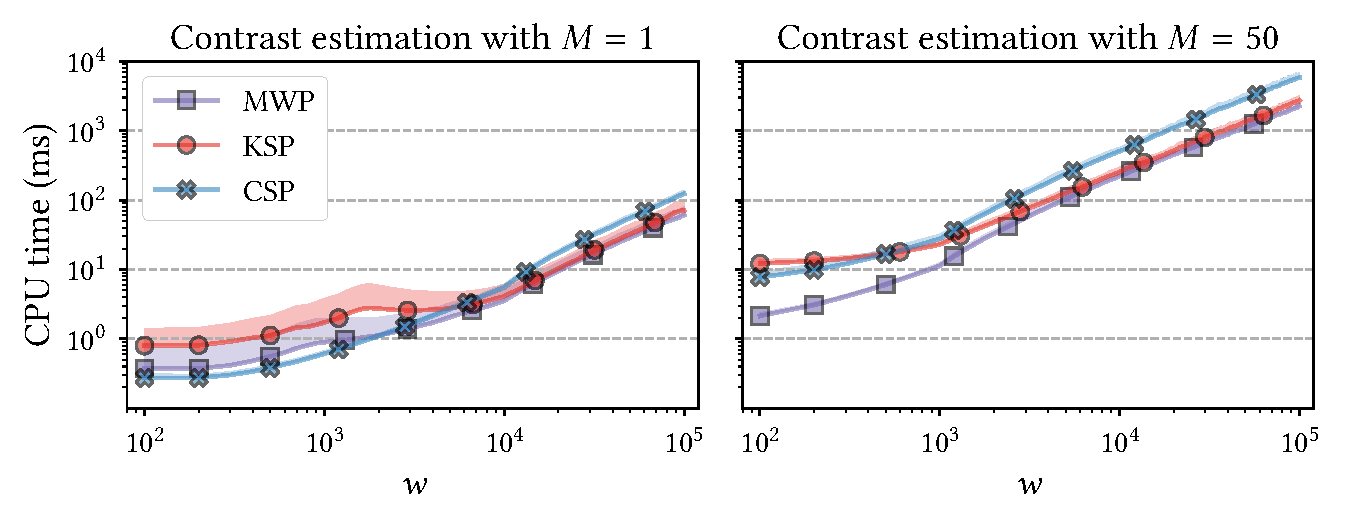
\includegraphics[width=\linewidth]{part2-figures/contrastperformance_thesis-compressed.pdf}
    \caption{Time required for contrast estimation w.r.t. window size $\gls{w}$.}
    \label{fig:scalability-contrast}
\end{figure} 

\subsubsection{Deployment to the Streaming Setting}

We monitor contrast when the dependency gradually evolves. 
We simulate this setting by concatenating $100$ three-dimensional linear dependencies with $1\,000$ observations each and a level of noise $\sigma$ 
linearly increasing from $0$ to $1$. 
We use the approach described in Section \ref{adaptation-stream}, Equation \ref{eq:exp-decay} and instantiate \gls{MCDE} with \gls{MWP}. We estimate the dependency over a sliding window of size  $w=1\,000$ and with a decaying factor $\gamma = 0.99$. 

We let $\Delta$ vary from $1$ to $1\,000$ and $M$ from $1$ to $500$. 
We compare each configuration to a baseline, which is the most expensive configuration ($\Delta=1$, $M=500$), without the benefit of our update operations. 
When $\Delta > 1$, we simply set the current contrast estimate to the value from the latest estimation. We define the following measures: 
\begin{itemize}[noitemsep]
    \item The \textbf{Absolute Error} is the average absolute difference between the values obtained with the tested configuration and the values from the baseline. 
    \item The \textbf{Relative Time} is the ratio of the time required by the tested con\-fi\-gu\-ra\-tion over the time required by the baseline.
    \item The \textbf{Index Speedup} is the ratio between the time required by the tested configuration without/with our index update operations.  
\end{itemize}

We can see from Figure \ref{fig:stream-experiment} that the absolute error decreases with $\Delta$, while the relative execution time increases. 
The speedup obtained by our index operations is responsible for this gain in efficiency to a large part. 
As we increase the number of iterations $M$, the errors tend to decrease, but at the same time, contrast estimation dominates the overall execution time. 
In such cases, we see less benefit from our efficient insert/delete operations. 

We identify the configuration $M=50$, $\Delta=50$ as a sweet spot: for an absolute error as small as $\approx0.01$, the computational burden is reduced by up to $100$ times, with a consistent index speedup of $3$. We mark this configuration with a star $*$ in the figure. 
 
\begin{figure}
	\centering
    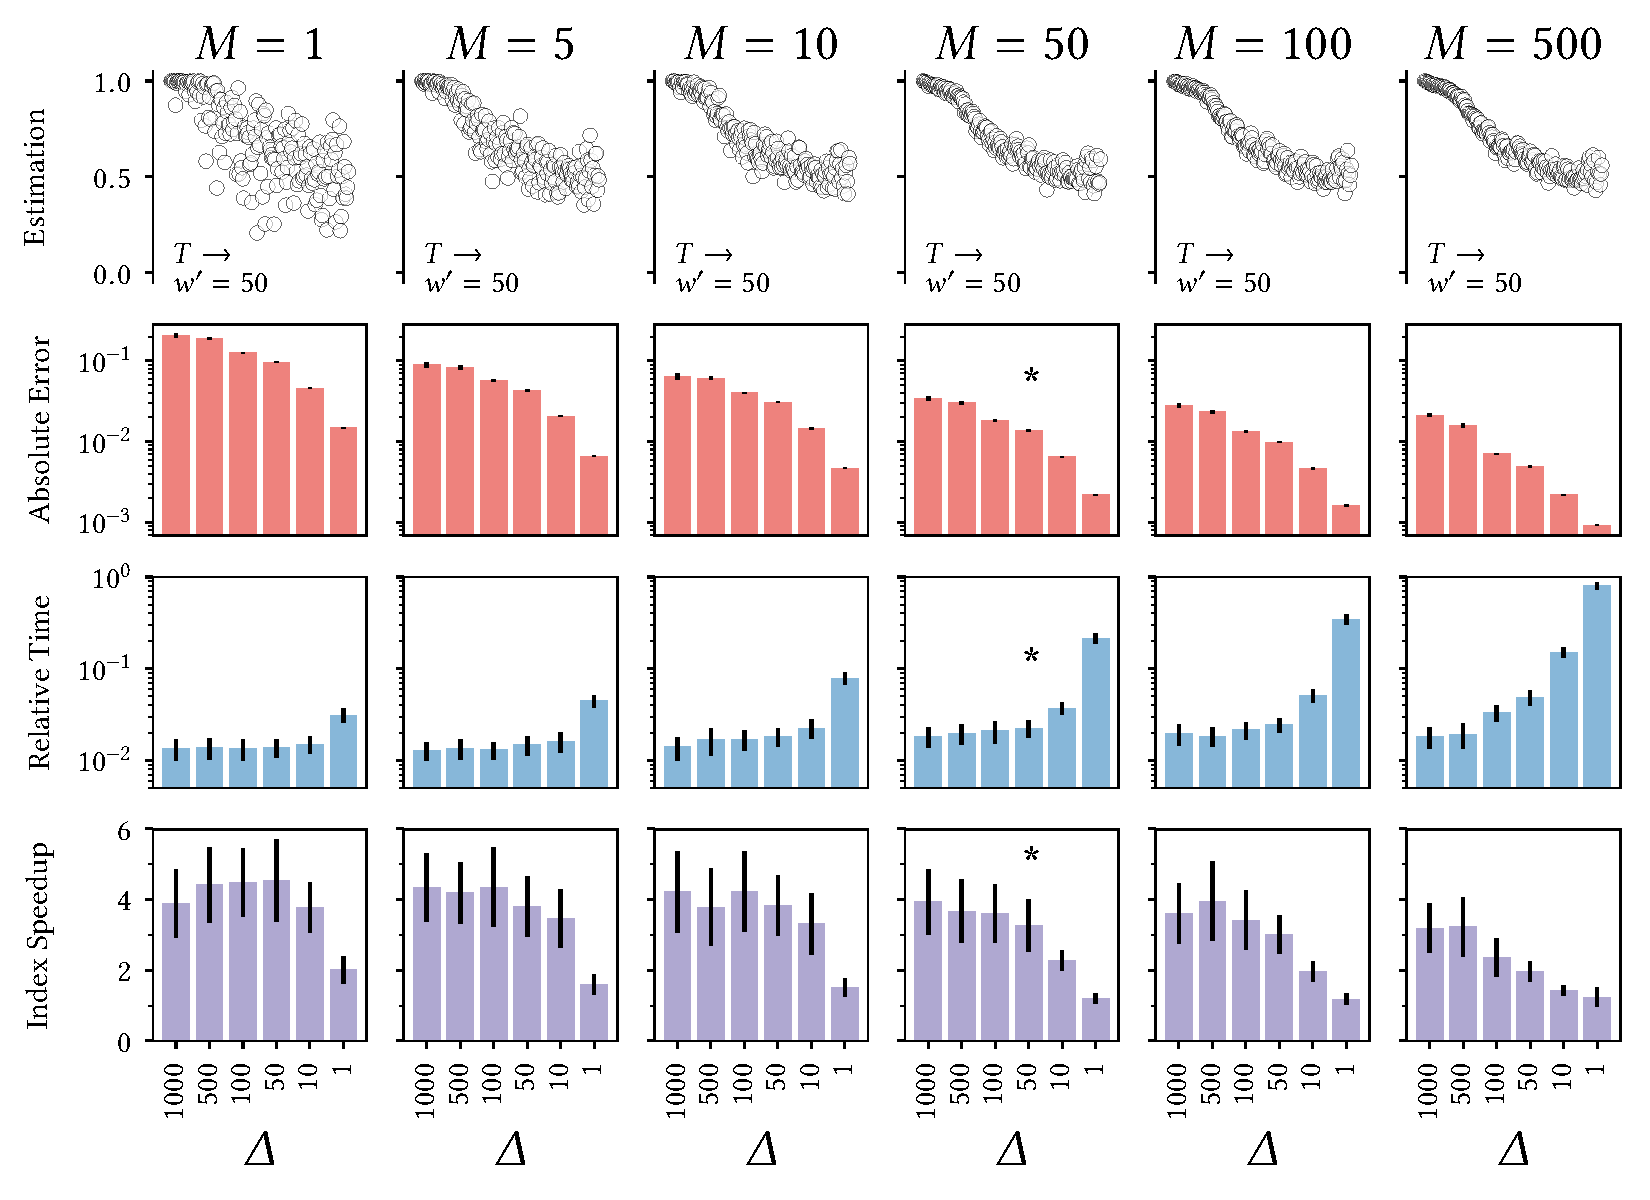
\includegraphics[width=\linewidth]{part2-figures/all_thesis-compressed.pdf}
    \caption{Performance of contrast estimation with \textit{concept drift} (* $\equiv$ sweet spot).}
    \label{fig:stream-experiment} 
\end{figure} 

\subsection{Case Study: Discovering Dependency Patterns}

\glsunset{Bioliq}
We now apply \gls{MCDE} to a real-world multivariate time series. 
The data was collected during a 4-day production campaign at \gls{Bioliq}, a pyrolysis plant in the surroundings of Karlsruhe  \cite{pfitzer2016fast}. It contains one measurement per second, i.e., $345\,600$ observations, from a selection of 20 physical sensors %, such as temperature or pressure, 
in various components of the plant. 
We monitored the evolution of dependency between each sensor pair with $\gls{w} = 1000,  \Delta = 50$, $M=50$, as just explained. 
We obtained the evolution of dependency between the $20$ sensors (i.e., $190$ pairs) using a single CPU core in about $2$ hours. Note that it would be easy to shorten the computation time significantly by parallel processing.  

We have presented the results of our monitoring technique to the plant operators. 
They have identified several patterns which they deemed `interesting', i.e., patterns yielding insights that could help with plant operation. 

Figure \ref{fig:real-world-pattern} displays one of these patterns. 
It is the result of monitoring two sensors, namely the pressure at the reactor input, and the oxygen concentration at the output. 
As we see, the dependency between these two measures changes significantly over time. 
Some changes, marked in the figure from 1 to 4, appear to represent different stages in the production process. 
A better understanding of the dynamics of the physical measures involved in the reaction will help the plant owners to operate smoothly and efficiently. 

\begin{figure}
\centering
    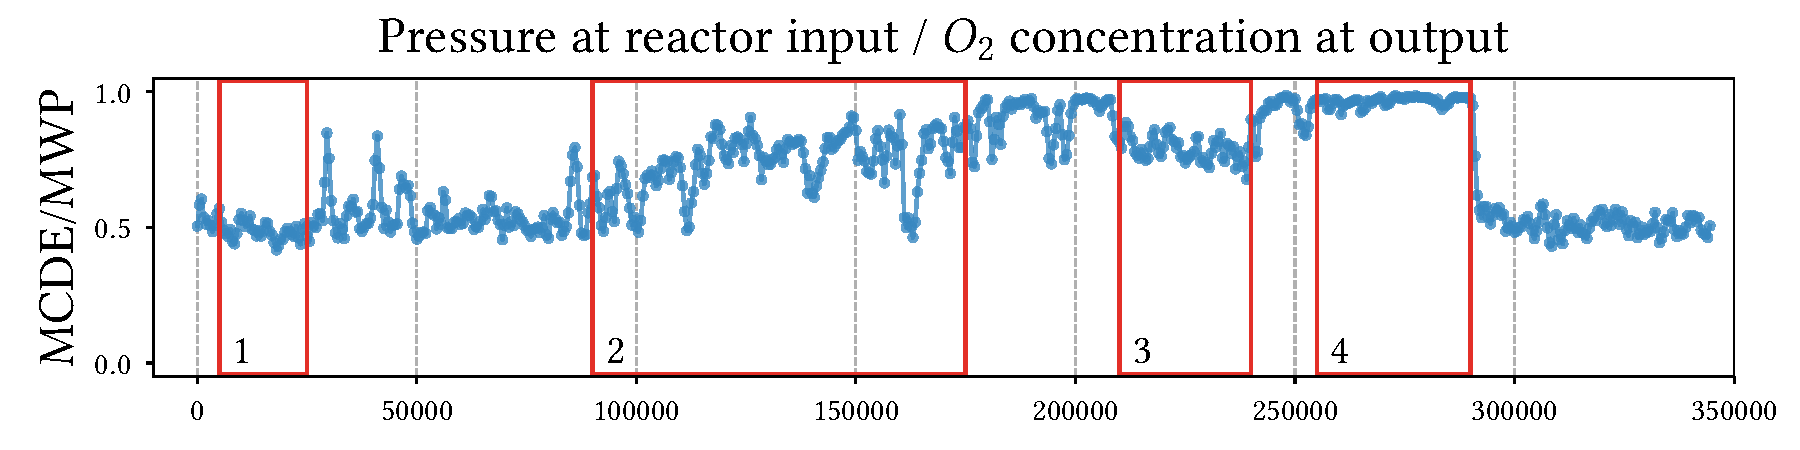
\includegraphics[width=1\linewidth]{part2-figures/Dep_example_thesis-compressed.pdf}
    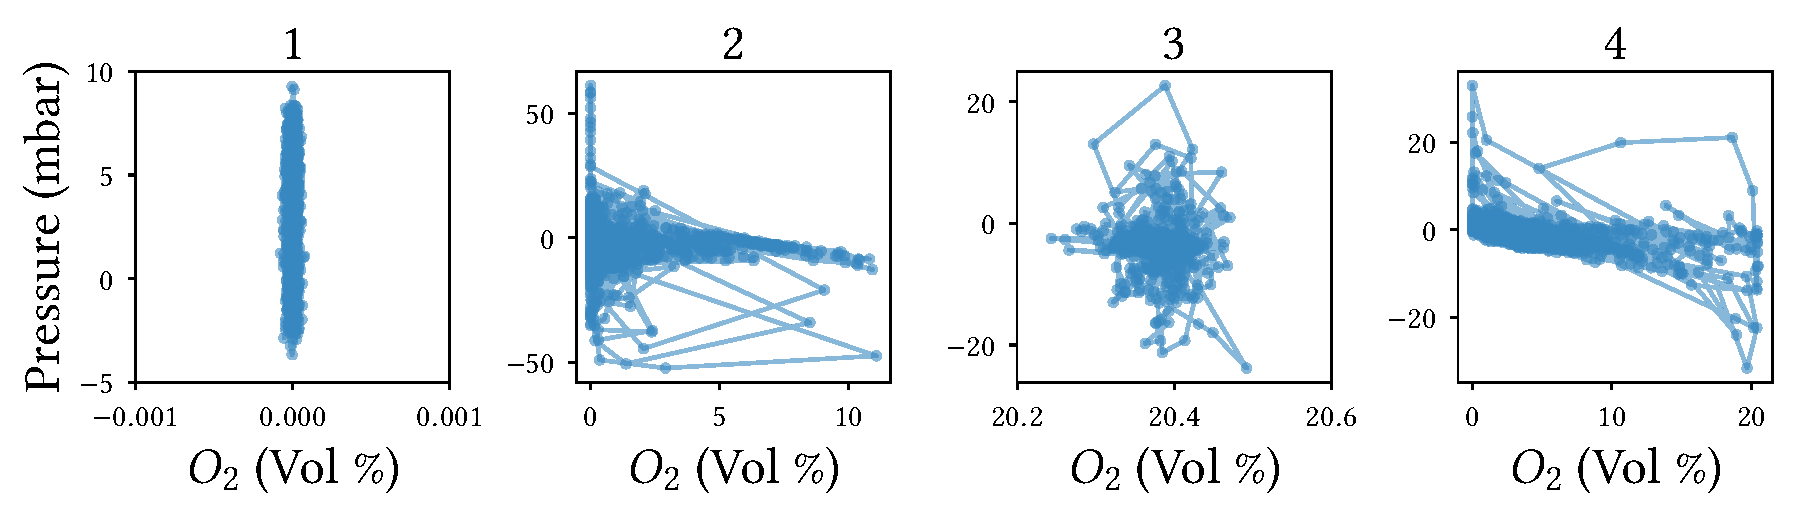
\includegraphics[width=1\linewidth]{part2-figures/Dep_example_details_thesis-compressed.pdf}
    \caption{Example of an interesting dependency pattern in the pyrolysis data.}
    \label{fig:real-world-pattern}
\end{figure}

\section{Discussion}

Our experiments show that \gls{MCDE} fulfils all requirements linked to heterogeneous data streams and has the desirable features of a framework for dependency estimation. %Each MCDE instantiations (MWP, KSP and CSP) are state of the art dependency estimators, which we can combine to tackle the challenging H-DS setting. 

First, we can see that \gls{MCDE} is efficient (\hyperlink{C1}{\textbf{C1}}), and, thanks to the index update operations, one can use it in combination with the sliding window model to mine data streams in a single scan (\hyperlink{C2}{\textbf{C2}}) and adapt (\hyperlink{C3}{\textbf{C3}}) the contrast estimation over time, taking \textit{concept drift} into account. 
Second, one can also reduce or increase the number of MC iterations $M$ to trade between accuracy and computation time, in an anytime (\hyperlink{C4}{\textbf{C4}}) fashion. \gls{MCDE} can handle heterogeneity (\hyperlink{C5}{\textbf{C5}})  via the instantiation of various statistical tests.

Each approach, except \gls{MCDE} and \gls{MS}, has at least one unintuitive parameter (\hyperlink{R3}{\textbf{R3}}): \gls{TC} and \gls{II} require $k \in \mathbb{N}$, \gls{CMI} requires $Q \in \mathbb{N}$, \gls{MAC} requires $\epsilon \in (0,1)$, \gls{UDS} requires $\beta \in \mathbb{N}$, \gls{HiCS} requires $\alpha \in (0,1)$. Next, only \gls{MCDE} and \gls{HiCS} allow trading accuracy for a computational advantage (\hyperlink{C4}{\textbf{C4}}). Note that, by adapting recent anytime estimators for \gls{MI} such as \cite{DBLP:conf/edbt/VollmerB19}, \gls{TC} and \gls{II} maybe potentially also fulfil \hyperlink{C4}{\textbf{C4}}. 

Last, \gls{MCDE} is non-parametric (\hyperlink{R4}{\textbf{R4}}) and interpretable (\hyperlink{R5}{\textbf{R5}}) by design. 
Our experiments against an assortment of dependencies show that it is multivariate (\hyperlink{R1}{\textbf{R1}}), general-purpose (\hyperlink{R2}{\textbf{R2}}) and robust (\hyperlink{R7}{\textbf{R7}}). \gls{MCDE} is sensitive (\hyperlink{R6}{\textbf{R6}}) because estimates are the average of $\overline{p}$-values. Table~\ref{table:requirements} summarises our findings.

\begin{table}[ht]
	\caption{Fulfilment of Constraints and Requirements.} 
	%\footnotesize
	\centering
	\small
	\setlength\extrarowheight{-4pt}
	\begin{tabular}{l | c c c c c | c c c c c c c} 
		\toprule 
		Estimator 		&\hyperlink{C1}{\textbf{C1}}	& \hyperref[C2]{\textbf{C2}} 	& \hyperlink{C3}{\textbf{C3}} &\hyperref[C4]{\textbf{C4}} &\hyperref[C5]{\textbf{C5}}	& \hyperlink{R1}{\textbf{R1}}	& \hyperlink{R2}{\textbf{R2}}  & \hyperlink{R3}{\textbf{R3}}	& \hyperlink{R4}{\textbf{R4}}	& \hyperlink{R5}{\textbf{R5}} 	& \hyperlink{R6}{\textbf{R6}}	& \hyperlink{R7}{\textbf{R7}} \\ 
		\midrule 
		\gls{MS} 	& ++ 			& \xmark 		& \xmark	& \xmark & \xmark 		& \cmark      	& \xmark 		& \cmark 	& \cmark 		& \cmark 		& \xmark		& \cmark \\ 
		\gls{TC} 	& -				& \cmark 		& \cmark 	& \cmark & \xmark 		& \cmark 		& \cmark 		& \xmark 	& \cmark 		& \xmark 		& \cmark		& \xmark \\
		\gls{II} 	& -{}- 			& \cmark 		& \cmark 	& \cmark & \xmark 		& \cmark 		& \xmark 		& \xmark 	& \cmark 		& \xmark 		& \xmark 		& \xmark \\
		\gls{CMI} 	& + 			& \xmark 		& \xmark 	& \xmark & \xmark 		& \cmark 		& \xmark 		& \xmark 	& \cmark 		& \xmark 		& \xmark		& \xmark \\
		\gls{MAC} 	& -{}- 			& \xmark 		& \xmark 	& \xmark & \xmark 		& \cmark 		& \xmark 		& \xmark 	& \cmark 		& \xmark 	 	& \xmark		& \cmark \\
		\gls{UDS} 	& - 			& \xmark 		& \xmark 	& \xmark & \xmark		& \cmark 		& \xmark  		& \xmark 	& \cmark 		& \xmark 		& \xmark		& \cmark \\ 
		\gls{HiCS} 	& +				& \xmark 		& \xmark 	& \cmark & \xmark		& \cmark 		& \cmark 		&  \xmark 	& \cmark 		& \xmark 		& \xmark		& \xmark \\ 
		\gls{MCDE} 	& ++ 			& \cmark 		& \cmark	& \cmark & \cmark		& \cmark 		& \cmark 		& \cmark 	& \cmark 		& \cmark 		& \cmark		& \cmark \\
		\bottomrule
	\end{tabular}
	\label{table:requirements}
\end{table}
 
All in all, \gls{MCDE} yields to state-of-the-art estimators: it is versatile, allowing quality-runtime trade-offs and parallelisation, which is useful when time is critical, e.g., in large data streams. At the same time, it shows excellent detection quality with no restriction on the dependency type, while being easy to use and interpret. \gls{MCDE} features a blend of properties that so far no competitor offers. 

In this chapter, we have described a framework to estimate multivariate dependency in heterogeneous data streams. 
It fulfils all requirements one would expect from a state-of-the-art dependency estimator. 
Compared to other approaches, it provides high statistical power on a large panel of dependencies, while being very efficient. Furthermore, we introduced index operations for the streaming setting and illustrated the benefits of our framework against a real-world use case. In the next part, we generalise the task of dependency estimation to monitoring large sets of statistics. 

\part{Monitoring}
\label{partIII}

\chapter{\acrlong{S-MAB} Algorithms}
\glsresetall
\label{chapter:S-MAB}

The content of this chapter bases on the following publication: 
\begin{itemize}[noitemsep]
	\item \fullcite{DBLP:conf/kdd/FoucheKB19}
\end{itemize}
\textbf{Keywords:} Bandit Algorithms; Thompson Sampling; Adaptive Windowing%; Data Stream Monitoring; Predictive Maintenance

\section{Chapter Overview}

The \gls{MAB} is a fundamental model capturing the dilemma between exploration and exploitation in sequential decision-making. 
At every time step, the decision-maker selects a set of arms and observes a reward from each of the chosen arms. 
In this chapter, we present a variant of the problem, which we call the \gls{S-MAB}: the goal of the decision-maker is not only to maximise the cumulative rewards, i.e., choosing the arms with the highest expected reward, but also to decide how many arms to select so that, in expectation, the cost of selecting arms does not exceed the rewards. 
This problem is relevant to many real-world applications, e.g., online advertising, financial investments or data stream monitoring. In Section \ref{section:notationsbandits}, we introduced the required notation to describe and analyse our algorithms. This chapter makes the following contributions:  

\textbf{We address the \gls{S-MAB} problem, a novel generalisation of the \gls{MAB} problem.} The novelty is that the decision-maker not only decides which arms to play, but also how many, to maximise her cumulative reward under an efficiency constraint. 
To our knowledge, we are the first to consider this setting.   

\textbf{We first propose \gls{S-TS}, an algorithm to solve this problem in the static setting}, i.e., when the distribution of rewards does not change over time. 
We leverage existing bandit algorithms, e.g., \gls{TS}, and show that the regret of our method (i.e., the difference from the outcome of a perfect oracle) %EF: Note that here we do not only talk about expected rewards, regret in our case is also "pull regret" so "outcome" is more general.
only grows logarithmically with the number of time steps. 

\textbf{Then, we generalise our method for the non-static setting.} To do so, we combine our algorithm with \gls{ADWIN}, a state-of-the-art change detector, which is at the same time efficient and offers theoretical guarantees. 

\textbf{Finally, we validate our findings via experiments.} We illustrate the benefits of our contribution via a real-world use case on predictive maintenance. The comparison with existing approaches shows that our method achieves state-of-the-art results. 
-- We release our source code and data on GitHub\footnote{\url{https://github.com/edouardfouche/S-MAB}}, to ensure reproducibility.

\section{\acrlong{S-TS}}
\label{sec:STS}

Let us first assume a static environment. Our algorithm consists of: 
\begin{enumerate}[noitemsep]
	\item A \gls{MP-MAB} to identify the top-$\gls{L}_{\gls{t}}$ arms (\hyperlink{*1}{\textbf{*1}}). \label{component1}
	\item A so-called `scaling policy', to determine the value of $\gls{L}_{\gls{t}+1}$ based on $\gls{L}_{\gls{t}}$ and the observations at time $\gls{t}$ (\hyperlink{*2}{\textbf{*2}}). \label{component2}
\end{enumerate}

For (\ref{component1}), we use an existing algorithm, \gls{MP-TS}. It is a Bayesian-inspired bandit algorithm, which maintains a Beta posterior with parameters $\alpha_i, \beta_i$ over each arm $i$. In each round, \gls{MP-TS} samples an observation $\theta_i$ from each posterior and selects the top-$\gls{L}_{\gls{t}}$ arms according to these observations. Then, the parameters of this posterior are adjusted based on the reward vector $\gls{X(t)}$. 

%Our experiments (Section \ref{evaluation}) will show that MP-TS yields better results than MP-MAB based on UCB \cite{Chen2016}, KL-UCB \cite{garivier2018kl} and Exp3 \cite{auer1995gambling}. 

For (\ref{component2}), we propose to use a scaling policy, i.e., a strategy to control the number of plays, such that the empirical efficiency $\hat{\eta}_{\gls{t}}$ remains larger than $\gls{eta^*}$. Whenever $\hat{\eta}_{\gls{t}} \leq \gls{eta^*}$, we `scale down', i.e., we set $\gls{L}_{\gls{t}+1} = \gls{L}_{\gls{t}} - 1$. Otherwise, we `scale up'. 
When we are confident that adding one arm will lead to $\hat{\eta}_{\gls{t}} \leq \gls{eta^*}$, we stop scaling. 
To do so, we estimate $B_{\gls{t}}$, an upper confidence bound for $\hat{\eta}_{\gls{t}+1}$, assuming that $\gls{L}_{\gls{t}+1} = \gls{L}_{\gls{t}} + 1$. $\hat{B}_{\gls{t}}$ is our estimator for $B_{\gls{t}}$, based on the observations from the environment so far. The confidence is derived from the Kullback-Leibler divergence, as the so-called \gls{KL-UCB} index \cite{DBLP:journals/jmlr/GarivierC11,DBLP:conf/alt/Maillard17}. 
We name our policy  \gls{KL-S}:
\begin{align}
\label{scalingpolicy_analysis}
\gls{L}_{\gls{t}+1} = 
\begin{cases}
\gls{L}_{\gls{t}}-1 
&\quad\text{if } \hat{\eta}_{\gls{t}}  \leq  \gls{eta^*}  \\
\gls{L}_{\gls{t}}+1
&\quad\text{if } \hat{\eta}_{\gls{t}} >  \gls{eta^*} \text{ and } \hat{B}_{\gls{t}} >  \gls{eta^*}\\ 
\gls{L}_{\gls{t}}
&\quad\text{otherwise} \\ 
\end{cases}
\end{align}
where $1 \leq \gls{L}_{\gls{t}+1} \leq  \gls{K}$ and
\begin{align}
\hat{\eta}_{\gls{t}} = \frac{1}{\gls{L}_{\gls{t}}} \sum_{i}^{\gls{I(t)}} \hat{\mu}_i &&
\hat{B}_{\gls{t}} = \frac{\gls{L}_{\gls{t}}}{\gls{L}_{\gls{t}}+1} \hat{\eta}_{\gls{t}} + \frac{1}{\gls{L}_{\gls{t}}+1} b_{\widehat{\gls{L}_{\gls{t}}+1}}(\gls{t})
\end{align}
$\hat{B}_{\gls{t}}$ is the empirical estimator of 
\[
B_{\gls{t}} = \frac{1}{\gls{L}_{\gls{t}}+1} \sum_{i=1}^{\gls{L}_{\gls{t}}} \gls{mu_i}(\gls{t}) + \frac{1}{\gls{L}_{\gls{t}}+1} b_{\gls{L}_{\gls{t}}+1}(\gls{t}).
\] 
where $b_i(\gls{t})$ is the  \gls{KL-UCB} index of arm $i$ and $\widehat{\gls{L}_{\gls{t}}+1}$ is the arm of the ($\gls{L}_{\gls{t}}+1$)-th largest index. The  \gls{KL-UCB} index is as follows: 
\begin{equation}
\label{kl-index}
b_i(\gls{t}) = \max_q \{  \gls{N_i(t)} \cdot d_{\text{KL}}(\hat{\mu}_i(\gls{t}), q) \le \log(\gls{t}/ \gls{N_i(t)})\}
\end{equation}
where $d_{\text{KL}}$ is the Kullback-Leibler divergence. Intuitively, our policy maximises $\gls{L}_{\gls{t}}$ such that the empirical efficiency $\hat{\eta}_{\gls{t}}$ remains larger than $ \gls{eta^*}$ at any time $\gls{t}$. We stop scaling up whenever $\hat{B}_{\gls{t}}$, which is an upper confidence bound of $\hat{\eta}_{\gls{t}}$, is greater than $ \gls{eta^*}$.

In  \gls{S-TS}, the algorithms of (\ref{component1})  \gls{MP-TS} and (\ref{component2})  \gls{KL-S} are intertwined. 
See Algorithm \ref{S-TS}.   \gls{S-TS} successively calls the two procedures  \gls{MP-TS} and  \gls{KL-S}, 
while maintaining the statistics $\gls{N_i(t)}, \gls{S_i(t)}$ for each arm. 
We initialise the scaling policy with $\gls{L}_1 =  \gls{K}$ (Lines~\ref{alg1line1}-\ref{alg1line2}).
The rationale is that nothing is known about the reward distribution of the arms initially, so pulling a maximum number of arms is informative. Previous studies showed that optimistic initialisation improves the empirical performance of bandit algorithms \cite{DBLP:journals/corr/KuleshovP14, DBLP:books/lib/SuttonB98}. 

\textbf{Computational complexity of Algorithm \ref{S-TS}:}
At each round,  \gls{MP-TS} draws a sample from a Beta distribution (Line \ref{betadrawing}), and  \gls{KL-S} computes the  \gls{KL-UCB} index for each arm (Line \ref{klindex-computation}), which can be done efficiently via Newton's method. 
Given that these operations are done in constant time and that finding the top-$\gls{L}_{\gls{t}}$ elements among $ \gls{K}$ elements takes $O( \gls{K} \log  \gls{K})$ in the worst case ($\gls{L}_{\gls{t}} =  \gls{K}$), each round of the proposed algorithm takes $O( \gls{K} \log  \gls{K})$ time. Therefore, the total computational complexity of the algorithm is $O(\gls{T} \gls{K} \log(\gls{K}))$.
The space complexity of the algorithm is $O( \gls{K})$, as it only keeps four statistics ($\alpha_i$, $\beta_i$, $N_i$, $S_i$) per arm $i \in [ \gls{K}]$. 

\begin{algorithm}
	\footnotesize
	\caption{ \gls{S-TS}($[\gls{K}], \eta^*$)}\label{S-TS} 
	\begin{algorithmic}[1]
		\Require Set of arms
		$[\gls{K}] = \{1,2,\dots, \gls{K}\}$, target efficiency $ \gls{eta^*}$
		\State $\alpha_i(1) = 0$, $\beta_i(1) = 0$ \quad $\forall i \in [ \gls{K}]$ \label{alg1line1}
		\State $N_i(1) = 0$, $S_i(1) = 0$ \quad $\forall i \in [ \gls{K}]$  \label{alg1line2}
		\State $\gls{L}_1 \gets  \gls{K}$ 
		\For{$t = 1,2,\dots,\gls{T}$}
		\State $ \gls{I(t)},  \gls{X(t)} \gets $ \Call{ \gls{MP-TS}}{$\gls{L}_{\gls{t}}$} \Comment{Play $\gls{L}_{\gls{t}}$ arms (as in  \gls{MP-TS})}
		\For{$i \in  \gls{I(t)}$}
		\State $N_i(\gls{t}+1) =  \gls{N_i(t)} + 1$
		\State $S_i(\gls{t}+1) =  \gls{S_i(t)} +  \gls{X_i(t)}$
		\EndFor
		\State $\gls{L}_{\gls{t}+1} \gets$ \Call{ \gls{KL-S}}{$\gls{L}_{\gls{t}}$} \Comment{Scale $\gls{L}_{\gls{t}}$ for the next round}
		\EndFor
		\Statex~
		\Procedure{ \gls{MP-TS}}{$\gls{L}_{\gls{t}}$} \label{line_mpts}
		\For{$i = 1,\dots, \gls{K}$}  
		\State $\theta_i(\gls{t}) \sim \text{Beta}(\alpha_i(\gls{t})+1, \beta_i(\gls{t})+1)$ \label{betadrawing}
		\EndFor 
		\State Play arms $ \gls{I(t)} := \argmax_{K' \subset [ \gls{K}], |K'| = \gls{L}_{\gls{t}}} \sum_{i}^{K'}\theta_i(\gls{t})$ \label{sorting-theta}
		\State Observe reward vector $ \gls{X(t)}$
		\For{$i \in  \gls{I(t)}$} \Comment{Update parameters}
		\State $\alpha_i(\gls{t}+1) = \alpha_i(\gls{t}) +  \gls{X_i(t)}$ 
		\State $\beta_i(\gls{t}+1) = \beta_i(\gls{t}) + (1- \gls{X_i(t)})$ 
		\EndFor
		\State \textbf{return} $ \gls{I(t)},  \gls{X(t)}$
		\EndProcedure
		\Statex~
		\Procedure{ \gls{KL-S}}{$\gls{L}_{\gls{t}}$}
		\State $S_i = S_i(\gls{t}+1), N_i = N_i(\gls{t}+1) \quad \forall i \in [ \gls{K}]$
		\State $\hat{\mu}_i = S_i/N_i \quad \forall i \in [ \gls{K}]$ \Comment{$\hat{\mu}_i = 1$, if $N_i = 0$}
		\State $\hat{\eta}_{\gls{t}} = \sum_{i \in  \gls{I(t)}} \hat{\mu}_i$
		\If{$\hat{\eta}_{\gls{t}} \leq  \gls{eta^*}$} \textbf{return} $\max(\gls{L}_{\gls{t}} - 1, 1) $
		\Comment{Scale down}
		\Else{
			\State  $KL = \left \{	\max_q \{ N_i\cdot d_{\text{KL}}(\hat{\mu}_i, q) \le \log\frac{\gls{t}+1}{N_i}\}: \forall i \in [ \gls{K}] \right\}$ \label{klindex-computation}
			\State $b_{\widehat{\gls{L}_{\gls{t}} +1}} = (\gls{L}_{\gls{t}} + 1)$-th largest element from $KL$ \label{sorting-kl}
			\State $\hat{B}_{\gls{t}}$ = $\frac{\gls{L}_{\gls{t}}}{\gls{L}_{\gls{t}} + 1} \hat{\eta}_{\gls{t}} + \frac{1}{\gls{L}_{\gls{t}} + 1} b_{\widehat{\gls{L}_{\gls{t}} + 1}}(\gls{t})$
			\If{$\hat{B}_{\gls{t}} >  \gls{eta^*}$}  \textbf{return} $\min(\gls{L}_{\gls{t}} + 1,  \gls{K})$ \Comment{Scale up}
			\Else ~\textbf{return} $\gls{L}_{\gls{t}}$ \Comment{Do not scale}
			\EndIf
		}
		\EndIf
		\EndProcedure
	\end{algorithmic}
\end{algorithm}

\section{\acrlong{S-TS-ADWIN}}
\label{non-static-adaptation}

To handle the non-static setting (\hyperlink{*3}{\textbf{*3}}), we combine  \gls{S-TS} with \gls{ADWIN} \cite{DBLP:conf/sdm/BifetG07}. We call the resulting algorithm \gls{S-TS-ADWIN}.

\gls{ADWIN} (Algorithm \ref{ADWIN}) monitors the expected value from a single (virtually infinite) stream of values $\{x_1,x_2,\dots\}$, where $x_i \in [0,1]$. 
\gls{ADWIN} maintains a window $W$ of varying size $|W| = \gls{w}$ so that the nature of the stream is consistent. \gls{ADWIN} reduces the size of the window whenever two neighbouring subwindows have different mean, based on a statistical test with %a given
confidence $\delta$. %Let $t$ be the current time step. 
For every two subwindows of size $|W_1| + |W_2| = |W|$ with corresponding means $\hat{\mu}_{W_1},\hat{\mu}_{W_2}$, \gls{ADWIN} shrinks the windows to $W_2$ if 
\begin{equation}
 |\hat{\mu}_{W_1} - \hat{\mu}_{W_2}| \ge \epsiloncut^\delta \quad \mathrm{where} \quad \epsiloncut^\delta = \sqrt{\frac{1}{2 m} \log\left(\frac{4 |W|}{\delta}\right)}
\end{equation}
and $m = 1/((1/|W_1|)+(1/|W_2|))$. %EF: We don't need the detail on \delta' (simpler)
\cite{DBLP:conf/sdm/BifetG07} showed that \gls{ADWIN} efficiently adapts to both gradual and abrupt changes with theoretical guarantees %on the rates of false positives and false negatives 
(see Theorem 3.1 therein).

\begin{algorithm}
	\footnotesize
	\caption{\gls{ADWIN}($B$, $\delta$)}\label{ADWIN} 
	\begin{algorithmic}[1]
		\Require Stream of values $B = (x_{1}, x_{2}, \dots)$, confidence level $\delta$ 
		\State $W \leftarrow \{\}$
		\For{$t = 1,2,\dots$}
		\State $W \leftarrow W \cup \{x_{\gls{t}}\}$
		\State Drop elements from the tail of $W$ until $|\hat{\mu}_{W_1} - \hat{\mu}_{W_2}| < \epsiloncut^\delta$ holds for every split $W = W_1 \cup W_2$. 
		\EndFor
	\end{algorithmic}
\end{algorithm}

The idea behind \gls{S-TS-ADWIN}, showed in Algorithm \ref{S-TS-ADWIN}, is to create an \gls{ADWIN}  instance $A_i$ per arm $i$.
At each step $t$, $A_i$ obtains as input the reward from the corresponding arm $\gls{X_i(t)}$ if $i \in \gls{I(t)}$. 
Thus, each instance $A_i$ maintains a time window $W_i$ of variable size, which shrinks whenever \gls{ADWIN} detects a change in $\gls{mu_i}$.  

However, for any bandit algorithm with logarithmic regret, the number of plays of suboptimal arms grows with $\log(\gls{T})$. 
That is, after some time, the $A_j$ of any suboptimal arm $j$ does not obtain any input, and thus no change can be detected for arm $j$. 

Thus, we use $\gls{w}_{\gls{t}} = \min\{|W_i|: \forall i \in [\gls{K}]\}$, i.e., the smallest window from each $A_i$, to estimate the statistics of any arm~$i \in [\gls{K}]$ at each step $\gls{t}$. 
Here, we implicitly assume that the change points are `global', i.e., that they are shared across the $\gls{mu_i}, \forall i \in [\gls{K}]$. In principle, changes may also be `local', e.g., a single $\gls{mu_i}$ changes. But we will show that despite this assumption, it works well in practice. %EF: That is not completely exact. It works well in our synthetic examples because the arms changing are top-arms. This would be a different story if suddenly suboptimal arm would become optimal. 

\begin{algorithm} 
	\footnotesize
	\caption{\acrshort{S-TS-ADWIN}($[\gls{K}], \gls{eta^*}, \delta$)}\label{S-TS-ADWIN} 
	\begin{algorithmic}[1]
		\Require Set of arms
		$[\gls{K}]$, target efficiency $\gls{eta^*}$, delta $\delta$
		%EF: We also initialise with 0 here. 
		\State $\alpha_i(1) = 0$, $\beta_i(1) = 0$ \quad $\forall i \in [\gls{K}]$  
		\State $\alpha_i(1) = 0$, $\beta_i(1) = 0$ \quad $\forall i \in [\gls{K}]$ 
		\State $\textit{N}_i(1) = 0$, $\textit{S}_i(1) = 0$ \quad $\forall i \in [\gls{K}]$ 
		\State$A_i \gets $ instantiate \gls{ADWIN} with parameter $\delta, \forall i \in [\gls{K}]$ \label{line3} 
		\State $\gls{L}_1 \gets \gls{K}$ 
		\For{$\gls{t} = 1,2,\dots,\gls{T}$}
		\State $\gls{I(t)}, \gls{X(t)} \gets $ \Call{\gls{MP-TS}}{$\gls{L}_{\gls{t}}$} \Comment{Play $\gls{L}_{\gls{t}}$ arms (as in \gls{MP-TS})}
		\For{$i \in \gls{I(t)}$}
		\State $N_i(\gls{t}+1) = \gls{N_i(t)} + 1$
		\State $S_i(\gls{t}+1) = \gls{S_i(t)} + \gls{X_i(t)}$
		\State\label{line10} Add $\gls{X_i(t)}$ into $A_i$
		\EndFor
		\State $\gls{L}_{\gls{t}+1} \gets$ \Call{\gls{KL-S}}{$\gls{L}_{\gls{t}}$} \Comment{Scale $\gls{L}_{\gls{t}}$ for the next round}
		\State\label{line11} $\gls{w}_{\gls{t}} \gets$ $ \min\{|W_i|: \forall i \in [\gls{K}]\}$ \Comment{Keep the smallest window}
		\State $N_i(\gls{t}+1) = \sum_{j = \gls{t} - w_{\gls{t}}}^{\gls{t}} \Ind(i \in I(j))$ 
		\State $S_i(\gls{t}+1) = \sum_{j = \gls{t} - \gls{w}_{\gls{t}}}^{\gls{t}} X_i(j) * \Ind(i \in I(j))$ 
		\State $\alpha_i(\gls{t}+1) = S_i(\gls{t}+1), \beta_i(\gls{t}+1) =  N_i(\gls{t}+1) - S_i(\gls{t}+1)$ 
		\EndFor
	\end{algorithmic}
\end{algorithm}

By default, we set $\delta = 0.1$ for each instance, since \cite{DBLP:conf/sdm/BifetG07} showed that it leads to a very low empirical false positive rate and good performance. 
We show in our experiments that this parameter does not have a significant impact on our results and that S-TS-ADWIN performs very well against synthetic and real-world scenarios.  

\textbf{Computational complexity of Algorithm \ref{S-TS-ADWIN}:} We use the improved version of \gls{ADWIN}, dubbed ADWIN2 \cite{DBLP:conf/sdm/BifetG07}. For a window of size $\gls{w}$, ADWIN2 takes $O(\log \gls{w})$ time per object. Since we have $\gls{K}$ instances of them, the time complexity of the ADWIN2 part is in $O(\gls{K} \log \gls{w}) = O(\gls{K} \log \gls{T})$ per round. The space complexity of ADWIN2 is in $O(\gls{w})$, but the window typically shrinks rapidly in the case of a non-static environment. We show in our experiments that the scalability of \gls{S-TS-ADWIN} is almost the same as \gls{S-TS}.

\section{Theoretical Analysis}

%After having established basic definitions, we divide our analysis into two parts: First we look at the static setting, i.e., for which the distribution of rewards $\mu_i$ do not change. Then, we extend our analysis to the non-static case. 
We analyse the properties of scaling bandits. In particular, we measure the capability of an algorithm to control the size of $\gls{L}_{\gls{t}}$ by introducing a quantity called `pull regret'.
Our analysis is general: we show that not only \gls{S-TS} (Algo\-rithm~\ref{S-TS}) but that \gls{KL-S}, combined with any \gls{MP-MAB} algorithm of logarithmic regret, has logarithmic pull regret. 
We introduce our notation in Sec\-tion~\ref{subsec_theory_prelim} and proceed to our main theorem in Section \ref{regretbound}.

\subsection{The General Scaling Bandit}
\label{subsec_theory_prelim}
%Without loss of generality, we assume that $1 > \mu_1 > \mu_2 > \dots > \mu_K > 0$.
%Let $L^*$ be the largest number of pulls such that $\eta_t > \eta^*$. Namely, $L^* = \max_{l \in [K]} (1/l) \sum_{i=1}^l \mu_i > \eta^*$. 
We assume there is a unique $\gls{L^*}$, such that 
$\sum_{i=1}^{\gls{L^*}} \gls{mu_i}/\gls{L^*} > \gls{eta^*}$ and $\sum_{i=1}^{\gls{L^*}+1} \gls{mu_i}/(\gls{L^*}+1) < \gls{eta^*}$. %JK: removed the case of \sum_{i=1}^{L^*} \mu_i/L^* = \eta^*: At least this is highly non-trivial...I am not sure the alg works in this case or not.
Let $\Delta = \min(\Delta_a, \Delta_b)$ be the `gap', i.e., the absolute difference between $\gls{eta^*}$ and the closest possible $\eta_{\gls{t}}$, with $\Delta_a = (\sum_{i=1}^{\gls{L^*}} \gls{mu_i}- \gls{eta^*}) > 0$ and $\Delta_b = (\gls{eta^*} - \sum_{i=1}^{\gls{L^*}+1} \gls{mu_i}) > 0$. 

Let us first generalise \gls{S-TS} in Algorithm \ref{S-Gen}. 
A `base bandit' (\textsc{MP-Base-Bandit}, Line \ref{line_mpbase}) is an abstract bandit algorithm that, given the reward information up to the last round and the current number of plays $\gls{L}_{\gls{t}}$, decides on $\gls{I(t)}$, i.e., which arms to draw, and returns the reward vector $\gls{X(t)}$ at each round $\gls{t}$.

\begin{algorithm}
	\footnotesize
	\caption{General Scaling Bandit ($[\gls{K}], \gls{eta^*}$)}\label{S-Gen} 
	\begin{algorithmic}[1]
		\Require Set of arms
		$[\gls{K}]$, target efficiency $\gls{eta^*}$
		\State $\textit{N}_i(1) = 0$, $\textit{S}_i(1) = 0$ \quad $\forall i \in [\gls{K}]$ 
		\State $\gls{L}_1 \gets \gls{K}$ 
		\For{$t = 1,2,\dots,\gls{T}$}
		\State $\gls{I(t)}, \gls{X(t)} \gets $ \Call{MP-Base-Bandit}{$\gls{L}_{\gls{t}}$} \Comment{Play $\gls{L}_{\gls{t}}$ arms} \label{line_mpbase}
		\For{$i \in \gls{I(t)}$}
		\State $N_i(\gls{t}+1) = \gls{N_i(t)} + 1$
		\State $S_i(\gls{t}+1) = \gls{S_i(t)} + \gls{X_i(t)}$
		\EndFor
		\State $\gls{L}_{\gls{t}+1} \gets$ \Call{\gls{KL-S}}{$\gls{L}_{\gls{t}}$} \Comment{Scale $\gls{L}_{\gls{t}}$ for the next round}
		\EndFor
	\end{algorithmic}
	
\end{algorithm}

If we set \textsc{MP-Base-Bandit} $\equiv$ \gls{MP-TS}, then Algorithm \ref{S-Gen} becomes Algorithm \ref{S-TS}. As an alternative to \gls{MP-TS}, one could consider for example \gls{MP-KL-UCB} (resp.\ \gls{CUCB}) that draws the top-$\gls{L}_{\gls{t}}$ arms in terms of the \gls{KL-UCB} indices (resp.\ \gls{UCB} indices) or \gls{Exp3.M} that uses exponential weighting. 

To evaluate whether our scaling strategy converges to the optimal number of pulls $\gls{L^*}$, we define a new notion of `pull regret' as the absolute difference between the number of pulls $\gls{L}_{\gls{t}}$ and $\gls{L^*}$: 
\begin{align}
\text{PReg}(\gls{T}) = \sum_{\gls{t}=1}^{\gls{T}}  \left| \gls{L^*} - \gls{L}_{\gls{t}} \right|
\end{align}
The `standard' multiple-play regret, with varying $\gls{L}_{\gls{t}}$, measures how many suboptimal arms the algorithm draws. It is defined as:
\begin{align} \label{ineq_regret}
\text{Reg}(\gls{T}) = \sum_{\gls{t}=1}^{\gls{T}}{\left[\max_{\mI \subseteq [\gls{K}], |\mI|=\gls{L}_{\gls{t}}} \sum_{i \in \mI} \gls{mu_i} - \sum_{i \in \gls{I(t)}} \gls{mu_i} \right]}
\end{align}
Notice that, when an algorithm uses $\gls{L}_{\gls{t}} = \gls{L^*}$ in each round, 
the pull regret is $0$, and the regret boils down to the existing \gls{MP-MAB}. 
Achieving sublinear pull regret means that the algorithm satisfies the efficiency constraint, while sublinear regret means that it maximises the total reward, so we need to minimise both regrets. 

\subsection{Regret Bound}

\subsubsection{Logarithmic Regret} 

\label{regretbound}
For any event $\mX$, let $\mX^c$ be its complementary. For $\mX$, $\Ind(\mX) = 1$ if $\mX$ holds or $0$ otherwise.

\begin{definition}[Top-$\gls{L}_{\gls{t}}$ Set] 
$\gls{I(t)}: |\gls{I(t)}|=\gls{L}_{\gls{t}}$ is a top-$\gls{L}_{\gls{t}}$ set if it contains the $\gls{L}_{\gls{t}}$ arms with highest expectation $\gls{mu_i}$. Let $\mA_{\gls{t}}$ be the event that $\gls{I(t)}$ is the top-$\gls{L}_{\gls{t}}$ set. 
\end{definition}%
\begin{definition}[Logarithmic Regret Algorithm]\label{def_base} 
A base bandit algorithm has logarithmic regret if there exists a distribution-de\-pen\-dent constant $C_{\mathrm{alg}} = C_{\mathrm{alg}}(\{\gls{mu_i}\})$ such that 
\[
\sum_{\gls{t}=1}^{\gls{T}} \Pr\left[\mA^c_ {\gls{t}}\right] \le C^{\mathrm{alg}} \log \gls{T}
\] 
\end{definition}
\begin{remark}[Logarithmic Regret of Multiple-Play Bandits]\label{rem_co} Note that Definition \ref{def_base} is equivalent to state that the regret of Eq. \eqref{ineq_regret} is logarithmic. 
Based on the existing analyses \cite{DBLP:conf/nips/ChenHLLLL16}, one can prove that \gls{MP-KL-UCB} \cite{DBLP:journals/jmlr/GarivierC11} and \gls{MP-TS} \cite{DBLP:conf/icml/KomiyamaHN15} have logarithmic regret for varying $\gls{L}_{\gls{t}}$. For completeness, we show that \gls{MP-TS} has logarithmic regret in Section \ref{subsec_rem_mpts}, using techniques from \cite{DBLP:conf/aistats/AgrawalG13}. 
\end{remark}

The following theorem states that our policy has logarithmic pull regret, i.e., that the number of pulls converges to $\gls{L^*}$ when we combine it with a base bandit algorithm of logarithmic regret. 

\begin{theorem}[Logarithmic Pull Regret]
\label{thm_pullregret}
Let the general scaling bandit of Algorithm \ref{S-Gen} with a base bandit algorithm of logarithmic regret be given. Then, there exist two distribution-dependent constants $C_*^{\mathrm{preg}},C_*^{\mathrm{reg}} = C_*^{\mathrm{preg}}(\{\gls{mu_i}\}), C_*^{\mathrm{reg}}(\{\gls{mu_i}\})$ such that
\begin{equation}\label{ineq_pregsublin}
\mathbb{E}[\text{PReg}(\gls{T})] \le C_*^{\mathrm{preg}} \log \gls{T},
\end{equation}
Moreover, the standard regret of the proposed algorithm is bounded as
\begin{equation}\label{ineq_regsublin}
\mathbb{E}[\text{Reg}(\gls{T})] \le C_*^{\mathrm{reg}} \log \gls{T}.
\end{equation}
\end{theorem}%
Let us first define the events needed for the proof:
\begin{align}
\mB_{\gls{t}} &= \{\gls{L}_{\gls{t}} \le \gls{L^*} \cap \hat{\eta}_{\gls{t}} > \gls{eta^*}\} \cup \{\gls{L}_{\gls{t}} > \gls{L^*} \cap \hat{\eta}_{\gls{t}} \le \gls{eta^*}\} \\
\mC_{\gls{t}} &= \{\gls{L}_{\gls{t}} \ge \gls{L^*} \cup \hat{B}_{\gls{t}} > \gls{eta^*}\} \\
\mD_{\gls{t}} &= \{\gls{L}_{\gls{t}} < \gls{L^*} \cup \hat{B}_{\gls{t}} \le \gls{eta^*}\} 
\end{align}

The following lemmas are key to bound the pull regret: 
\begin{lemma}[Scaling]
	\label{lem_sufscalelb}
	$\gls{L}_{\gls{t}} \in \{\gls{L^*},\gls{L^*}+1\}$ holds if 
	\[
	\bigcap_{t' = \gls{t}-\gls{K},\dots,\gls{t}-1} \mB_{t'} \cap \mC_{t'}. 
	\]
\end{lemma}
\begin{proof}[Proof of Lemma \ref{lem_sufscalelb}]
	$\mB_{t'} \cap \mC_{t'}$ implies
	
	$\bullet \quad \gls{L}_{t'+1} = \gls{L}_{t'} + 1$ if $\gls{L}_{t'} < \gls{L^*}$, 
	
	$\bullet \quad \gls{L}_{t'+1} \in \{\gls{L^*}, \gls{L^*}+1\}$ if $L_{t'}=\gls{L^*}$
	
	$\bullet \quad \gls{L}_{t'+1} = \gls{L}_{t'} - 1$ if $\gls{L}_{t'} \ge \gls{L^*} + 1$ 
	
	As $\gls{L^*} - \gls{L}_{\gls{t}-\gls{K}} < \gls{K}$, there exists $t'_c \in \{\gls{t}-\gls{K},\gls{t}-\gls{K}+1,\dots,\gls{t}-1\}$ such that $\gls{L}_{t'_c} = \gls{L^*}$, and after the round $t'_c$, $\gls{L}_{t'} \in \{\gls{L^*},\gls{L^*}+1\}$ holds.  
\end{proof}
\begin{lemma}[Sufficient Condition of No-regret]
	\label{lem_sufnoregret}
	$\gls{L}_{\gls{t}} = \gls{L^*}$ holds if 
	\[
	\bigcap_{t' = \gls{t}-\gls{K},\dots,\gls{t}-1} \left\{\mB_{t'} \cap \mC_{t'}\right\} \cap \mD_{\gls{t}-1}.
	\]
\end{lemma}
\begin{proof}[Proof of Lemma \ref{lem_sufnoregret}]
	Lemma \ref{lem_sufscalelb} implies $\gls{L}_{\gls{t}-1} \in \{\gls{L^*},\gls{L^*}+1\}$, which, combined with $\mB_{\gls{t}-1} \cap \mC_{\gls{t}-1} \cap \mD_{\gls{t}-1}$ implies that, at round $\gls{t}-1$, it scales to $\gls{L}_{\gls{t}} = \gls{L^*}$.
\end{proof}
\clearpage
We can now proceed to the proof of Theorem \ref{thm_pullregret}:
\begin{proof}[Proof of Theorem \ref{thm_pullregret}]
Lemma \ref{lem_sufnoregret} implies that, if the direction of scaling is correct and the confidence bound is sufficiently small, then $\gls{L}_{\gls{t}}$ goes to $\gls{L^*}$. We decompose the pull regret using Lemma \ref{lem_sufnoregret}:
\begin{align}
\lefteqn{
	\text{PReg}({\gls{T}})  \le \gls{K} \sum_{\gls{t}=1}^{\gls{T}} \Ind[\gls{L}_{\gls{t}} \ne \gls{L^*}]
}\nn
&\ \ \text{(since $\text{PReg}(\gls{t})$ increases at most by $\gls{K}$ at each round)}\nn
&\le \gls{K} \sum_{\gls{t}=1}^{\gls{T}} \Ind\left[\left( \bigcup_{t'=\gls{t}-\gls{K}}^{\gls{t}-1} \left(\mA^c_{t'} \cup \mB^c_{t'} \cup \mC^c_{t'}\right) \cup \mD^c_{\gls{t}-1} \right) \cap \gls{L}_{\gls{t}} \ne \gls{L^*} \right] \nn
&\ \ \text{ (by the contraposition of Lemma \ref{lem_sufnoregret})}\nn
&\le \gls{K} + \gls{K} \sum_{\gls{t}=\gls{K}+1}^{\gls{T}} \Biggl( \Ind\left[\bigcup_{t'=\gls{t}-\gls{K}}^{\gls{t}-1} \left(\mA^c_{t'} \cup \mB^c_{t'} \cup \mC^c_{t'}\right)\right] \nn
&\ \ \ \ \ \ \ \ + \Ind\left[   \bigcap_{t'=\gls{t}-\gls{K}}^{\gls{t}-1} \left(\mA^c_{t'} \cap \mB^c_{t'} \cap\mC^c_{t'}\right) \cap \mD^c_{\gls{t}-1} \cap \gls{L}_{\gls{t}} \ne \gls{L^*} \right] \Biggr)\nn
&\le \gls{K} + \gls{K}^2 \sum_{t'=\gls{K}+1}^{\gls{T}} \left( \Ind[\mA^c_{t'}] + \Ind[\mA_{t'} \cap \mB^c_{t'}] + \Ind[\mA_{t'} \cap\mC^c_{t'}] \right) \nn
&\ \ + \gls{K} \sum_{\gls{t}=\gls{K}+1}^{\gls{T}} \Ind\left[ \bigcap_{t'=\gls{t}-\gls{K}}^{\gls{t}-1} \left(\mA_{t'} \cap \mB_{t'} \cap\mC_{t'}\right) \cap \mD^c_{\gls{t}-1} \cap \gls{L}_{\gls{t}} \ne \gls{L^*} \right] \label{preg_terms}
\end{align}
The following lemma bounds each term in Eq.\ \eqref{preg_terms} in expectation.

\begin{lemma}[Bounds on each Term] \label{lem_preg}
	The following bounds hold:
	\begin{align*}
	& \underbrace{\sum_{\gls{t}=1}^{\gls{T}} \Pr[\mA^c_{t'}]}_{\mathrm{(A)}} = O(\log \gls{T})  \quad;\quad \underbrace{\sum_{\gls{t}=1}^{\gls{T}} \Pr[\mA_{\gls{t}} \cap \mB^c_{\gls{t}}]}_{\mathrm{(B)}} = O(1/\Delta^2) \nn
	& \underbrace{\sum_{\gls{t}=1}^{\gls{T}} \Pr[\mA_{\gls{t}} \cap \mC^c_{\gls{t}}]}_{\mathrm{(C)}} = O(1/\Delta^2) + O(\log\log \gls{T}) \nn
	& \underbrace{\sum_{\gls{t}=\gls{K}+1}^{\gls{T}} \hspace{-0.5em}\Pr\left[ \bigcap_{t'=\gls{t}-\gls{K}}^{\gls{t}-1}\hspace{-0.5em} \left(\mA_{t'} \cap \mB_{t'}  \cap \mC_{t'}\right) \cap \mD^c_{\gls{t}-1}, \gls{L}_{\gls{t}} \ne \gls{L^*})\right]}_{\mathrm{(D)}}\hspace{-0.2em} =\hspace{-0.2em} O(1/\Delta^2). 
	\end{align*}
\end{lemma} 

Eq. \eqref{ineq_pregsublin} now follows from Lemma \ref{lem_preg}. Eq. \eqref{ineq_regsublin} follows from the fact that the base bandit algorithm has logarithmic regret. We will prove Lemma \ref{lem_preg} shortly after.
\end{proof}

\textbf{Discussion:} Following the bandit literature, we assume that parameters $\{\gls{mu_i}\}$ (and thus the gap $\Delta$) are constants. Although Lemma \ref{lem_preg} uses the Landau notation, all the terms\footnote{(including the involved underestimation term of Lemma \ref{lem_underest}, cf. \cite{DBLP:conf/alt/Maillard17} for an explicit bound)} in the analysis are explicitly written, i.e., they are finite-time. 
One can also see that the leading term of the pull regret and the regret are $O(\log {\gls{T}}/\Delta^2)$ when the regret of the base bandit algorithm (Definition \ref{def_base}) is $O(\log {\gls{T}}/\Delta^2)$: our scaling bandit algorithm targets at the largest $\gls{L}$ such that $(1/\gls{L})\sum_{i\le \gls{L}} \gls{mu_i} > \gls{eta^*}$, and the gap $\Delta$ characterises the hardness of finding such an $\gls{L}$. 
For ease of analysis, we omit the dependence on $\gls{K}$. 

In what follows, we show that Remark \ref{rem_co} holds for \gls{MP-TS}. Then, we prove Lemma \ref{lem_preg}. 

\subsubsection{Performance of \gls{MP-TS} as a `base bandit' algorithm}
\label{subsec_rem_mpts}

Let the posterior sample of \gls{TS} at round $\gls{t}$ be $\theta_i(\gls{t}) \sim \text{Beta}(\alpha_i(\gls{t})+1, \beta_i(\gls{t})+1)$.
Note that $\mA^c_{\gls{t}}, {\gls{T}} = l$ implies that there exists $i \le l$, $j > l$ such that $i \notin \gls{I(t)}$, $j \in \gls{I(t)}$.  Let $d = \gls{mu_i} - \mu_j > 0$ and $x, y = \mu_j + d/3, \mu_j + 2d/3$. Let the events $\mE_{i,\mu}(\gls{t}) = \{\hat{\mu}_i(\gls{t}) \le x \}$ and $\mE_{i,\theta}(\gls{t}) = \{\theta_i(\gls{t}) \le y\}$.
Let $\theta_{(l)}(\gls{t})$ be the $l$-th largest from $\{\theta_i(\gls{t})\}$ (ties are broken arbitrarily).
We have
\begin{align}
\sum_{\gls{t}=1}^{\gls{T}} \Pr\left[\mA^c_{\gls{t}}\right] 
&= \sum_{\gls{t}=1}^{\gls{T}} \sum_{l \in [\gls{K}]} \Pr\left[\mA^c_{\gls{t}} \cap {\gls{T}} = l\right] \nn
&\le \sum_{\gls{t}=1}^{\gls{T}} \sum_{l \in [\gls{K}]} \sum_{i \le l, j>l} \Pr\left[{\gls{T}} = l \cap i \notin \gls{I(t)} \cap j \in \gls{I(t)}\right].
\label{ineq_tsmain}
\end{align}
Here,
\begin{align}
\Pr&\left[{\gls{T}} = l \cap i \notin \gls{I(t)} \cap j \in \gls{I(t)}\right] \le \Pr\left[{\gls{T}} = l \cap y \le \theta_j(\gls{t})\right] 
\nn
&+ \Pr\left[{\gls{T}} = l \cap \theta_{(l)}(\gls{t}) \le y \cap \theta_i(\gls{t}) \le y\right].
\label{ineq_tsdecomp}
\end{align}
Let $p_{i,n} = \Pr[\theta_i(\gls{t}) > y \cap \gls{N_i(t)}=n]$.
The following discussion is essentially equivalent to Lemma 9 in \cite{DBLP:conf/icml/KomiyamaHN15}. 
Let $\theta_{(l)\setminus i}(\gls{t})$ be the value of the $l$-th largest among $\{\theta_j\}_{j \in [\gls{K}]\setminus i}$. Thus,
\begin{align*}
\lefteqn{
\sum_{\gls{t}=1}^{\gls{T}} \Ind\left[{\gls{T}} = l \cap \theta_{(l)}(\gls{t}) \le y \cap \theta_i(\gls{t}) \le y\right]
} \nn
&\le \sum_{n=1}^{\gls{T}} \sum_{\gls{t}=1}^{\gls{T}} \Ind\left[{\gls{T}} = l \cap \theta_{(l)}(\gls{t}) \le y \cap \theta_i(\gls{t}) \le y \cap \gls{N_i(t)}=n\right]\nn
&\le \sum_{n=1}^{\gls{T}} \sum_{\gls{t}=1}^{\gls{T}} \Ind\left[{\gls{T}} = l \cap \theta_{(l)\setminus i}(\gls{t}) \le y \cap \theta_i(\gls{t}) \le y \cap \gls{N_i(t)}=n\right]\nn
&\le \sum_{n=1}^{\gls{T}} \sum_{m=1}^{\gls{T}} \Ind\left[m \le \sum_{\gls{t}=1}^{\gls{T}} \Ind\left[{\gls{T}} = l \cap \theta_{(l)\setminus i}(\gls{t}) \le y \cap \theta_i(\gls{t}) \le y \cap N_i^{\gls{t}} =n\right] \right].
\end{align*} 
The event
\begin{equation}\label{ineq_underestm}
m \le \sum_{\gls{t}=1}^{\gls{T}} \Ind\left[\theta_{(l)\setminus i}(\gls{t}) \le y \cap \theta_i(\gls{t}) \le y \cap \gls{N_i(t)}=n\right] 
\end{equation}
implies that $\{\theta_{(l)\setminus i}(\gls{t}) \le y \cap \theta_i(\gls{t}) \le y \cap \gls{N_i(t)}=n\}$ occurred at least $m$ rounds, and $\{\theta_i(\gls{t}) \le y\}$ occurred for the first $m$ rounds such that Eq. \eqref{ineq_underestm} holds. 
By the statistical independence of $\theta_{(l)\setminus i}(\gls{t})$ and $ \theta_i(\gls{t})$, we have
\[
\Pr\left[m \le \Ind\left[{\gls{T}} = l \cap \theta_{(l)\setminus i}(\gls{t}) \le y \cap \theta_i(\gls{t}) \le y \cap N_i^{\gls{t}} =n\right] \right] \le (1 - p_{i,n})^m.
\]
and following the same steps as Lemma 9 in \cite{DBLP:conf/icml/KomiyamaHN15}, we have
\begin{align}
\sum_{n=1}^{\gls{T}} \sum_{m=1}^{\gls{T}} (1-p_{i,n})^m
&\le \sum_{n=1}^{\gls{T}} \frac{1-p_{i,n}}{p_{i,n}} \nn
&\le \frac{1}{(\gls{mu_i} - y)^2} \text{\ (by Lemma 2 in \cite{DBLP:conf/aistats/AgrawalG13})}. 
\label{ineq_tsunderestimate}
\end{align}
Moreover, by Lemma 4 and Lemma 3 in \cite{DBLP:conf/aistats/AgrawalG13}:
\begin{align}
&\Pr\left[{\gls{T}} = l \cap y \le \theta_j(\gls{t})\right] \le \Pr\left[{\gls{T}} = l \cap j \in \gls{I(t)} \cap y \le \theta_j(\gls{t}) \cap x > \hat{\mu}_j\right]
\nn
&\quad\quad\quad\quad\quad\quad\quad\quad\quad\quad + \Pr\left[{\gls{T}} = l \cap j \in \gls{I(t)} \cap x \le \hat{\mu}_j\right] \nn
&\le \left(\frac{\log \gls{T}}{\KL(x,y)} + 1\right) + \left(\frac{1}{\KL(x, \mu_j)} + 1\right),
\label{ineq_tsoverestimate}
\end{align}
where $\KL(p,q)=p\log(p/q)+(1-p)\log((1-p)/(1-q))$ be the KL divergence between two Bernoulli distributions. From Eqs. \eqref{ineq_tsmain}, \eqref{ineq_tsdecomp}, \eqref{ineq_tsunderestimate}, and \eqref{ineq_tsoverestimate},
$\sum_{\gls{t}=1}^{\gls{T}} \Pr\left[\mA^c_{\gls{t}}\right] = O(\log \gls{T})$.

\subsubsection{Proof of Lemma \ref{lem_preg}}
In this section, we bound each of the terms (A)--(D) in Lemma \ref{lem_preg}. Let us first describe the following required lemma:

\begin{lemma}[Uniform Bound] 
\label{lem_unifbound}

Let
\[
\mG_l(\gls{t}) = \bigcap_{i \le l}\left\{ |\hat{\mu}_i(\gls{t}) - \gls{mu_i}| \le \Delta \right\}.
\]
For $l \in [\gls{K}]$, the following inequality holds:
\begin{equation}
\sum_{\gls{t}=1}^{\gls{T}} \Pr[\mA_{\gls{t}} \cap {\gls{T}}=l \cap \mG_l^c(\gls{t}) ] = O(1/\Delta^2).
\end{equation}
\end{lemma}%
\begin{proof}[Proof of Lemma \ref{lem_unifbound}]
Event $\mA$ implies each arm $i \le l$ is drawn, and thus
\begin{align}
\lefteqn{
\sum_{\gls{t}=1}^{\gls{T}} \Pr[\mA_{\gls{t}} \cap {\gls{T}}=l \cap \mG_l^c(\gls{t}) ] 
\le 1 + \sum_{n=1}^{\gls{T}} \Pr[|\hat{\mu}_{i,n} - \gls{mu_i}| \le \Delta] 
}\nn
&\le 1 + \frac{1}{2 \Delta^2} \e^{-2 n_c \Delta^2}\ \text{(by Lemma \ref{lem_hp})} = O\left(\frac{1}{\Delta^2} \right). \qedhere
\end{align}
\end{proof}

\textbf{Bounding Term (A):} Term (A) is directly bounded by the fact that the base bandit algorithm has logarithmic regret.

\textbf{Bounding Term (B):}
Note that $\mB_{\gls{t}} = \{{\gls{T}} \le \gls{L^*} \cap \hat{\eta}_{\gls{t}} < \gls{eta^*}\} \cup \{{\gls{T}} > \gls{L^*} \cap \hat{\eta}_{\gls{t}} \ge \gls{eta^*}\}$, and $\{\mA_{\gls{t}} \cap \mG_l(\gls{t})\}$ implies $\mB_{\gls{t}}$. By Lemma \ref{lem_unifbound},
\begin{equation}
\sum_{\gls{t}=1}^{\gls{T}} \Pr[\mA_{\gls{t}} \cap \mB^c_{\gls{t}}] \le \sum_{l \in [\gls{K}]} \sum_{\gls{t}=1}^{\gls{T}} \Pr[\mA_{\gls{t}} \cap \mG_l^c(\gls{t})] = O(1/\Delta^2). \label{preg_terms_two}
\end{equation}
Note that $\mA_{\gls{t}} \cap L_{\gls{t}} = l$ implies arms $1,\dots,l$ are drawn.

\textbf{Bounding Term (C):}
The event $\mA_{\gls{t}} \cap B_i^l(\gls{t}) < \gls{eta^*}$ implies $\mG_l^c(\gls{t}) \cup b_{l+1}(\gls{t}) \le \mu_{l+1} - \Delta$. By using this, we have
\begin{align}
\lefteqn{
 \sum_{\gls{t}=1}^{\gls{T}} \Pr[\mA_{\gls{t}} \cap \mC^c_{\gls{t}}] \le \sum_{l = 1}^{\gls{L^*}-1} \sum_{\gls{t}=1}^{\gls{T}} \Pr[\mA_{\gls{t}} \cap {\gls{T}}=l \cap B_i^l(\gls{t}) \le \gls{eta^*}] } \nn
&\le \sum_{l = 1}^{\gls{L^*}-1} \sum_{\gls{t}=1}^{\gls{T}} \Pr\left[\mA_{\gls{t}} \cap {\gls{T}}=l \cap \left(\mG_l^c(\gls{t}) \cup b_{l+1}(\gls{t}) \le \mu_{l+1} - \Delta\right)\right] \nn
&\le \sum_{l = 1}^{\gls{L^*}-1} \sum_{\gls{t}=1}^{\gls{T}} \left( \Pr[\mA_{\gls{t}} \cap {\gls{T}}=l \cap \mG_l^c(\gls{t}))] + \Pr[b_{l+1}(\gls{t}) \le \mu_{l+1} - \Delta] \right)\nn
&\le \sum_{l = 1}^{\gls{L^*}-1} \sum_{\gls{t}=1}^{\gls{T}} \Pr[\mA_{\gls{t}} \cap {\gls{T}} = l \cap \mG_i^c(\gls{t}))] + O(\log\log \gls{T})\nn
&\ \ \text{\ (By the union bound of Lemma \ref{lem_underest} over $\gls{t} \in [\gls{T}]$)}\nn
&= O(1/\Delta^2) + O(\log\log \gls{T}) \quad \text{\ (by Lemma \ref{lem_unifbound})}.
\label{preg_terms_three}
\end{align}

\textbf{Bounding Term (D):}
Note that $\bigcap_{t'=\gls{t}-\gls{K}}^{\gls{t}-1} \left(\mA_{t'} \cap \mB_{t'} \cap \mC_{t'}\right)$ implies $\gls{L}_{\gls{t}-1} \in \{\gls{L^*}, \gls{L^*}+1\}$. Thus, ${\gls{T}} \ne \gls{L^*}$ implies $B_i^{\gls{L}_{\gls{t}-1}}(\gls{t}-1) > \gls{eta^*}$, and $B_i^{\gls{L}_{\gls{t}-1}}(\gls{t}-1) > \gls{eta^*}$ implies $\mG_{L_{\gls{t}-1}}^c(\gls{t}) \cup b_{\gls{L}_{\gls{t}-1}+1}(\gls{t}) > \mu_{\gls{L}_{\gls{t}-1}+1} + \Delta$. Moreover, $\bigcap_{t'=\gls{t}-\gls{K}}^{\gls{t}-1} \left(\mA_{t'} \cap \mB_{t'} \cap \mC_{t'}\right) \cap \mD^c_{\gls{t}-1}$ implies that arm $\gls{L^*}+1$ is drawn in either round $\gls{t}-1$ or round $\gls{t}$, and thus the event
\[
\bigcap_{t'=\gls{t}-\gls{K}}^{\gls{t}-1} \left(\mA_{t'} \cap \mB_{t'} \cap \mC_{t'}\right) \cap \mD^c_{\gls{t}-1} \cap N_{\gls{L^*}+1}(\gls{t})=n
\]
occurs at most twice for each $n$.

By using these, we obtain
\begin{align}
\lefteqn{
\sum_{\gls{t}=\gls{K}+1}^{\gls{T}} \Pr\left[ \bigcap_{t'=\gls{t}-\gls{K}}^{\gls{t}-1} \left(\mA_{t'} \cap \mB_{t'} \cap \mC_{t'}\right) \cap \mD^c_{\gls{t}-1} \cap {\gls{T}} \ne \gls{L^*})\right]
} \nn
&\le \gls{K} \sum_{l \in \{\gls{L^*}, \gls{L^*}+1\}}\sum_{\gls{t}=1}^{\gls{T}} \Pr[\mA_{\gls{t}} \cap \mG_l^c(\gls{t})] + \gls{K} + \frac{4\log \gls{T}}{\Delta^2}\nn
&\ \ \  + \sum_{\gls{t}=\gls{K}+1}^{\gls{T}} \Pr\left[b_{\gls{L^*}+1}(\gls{t}-1) \ge \mu_{\gls{L^*}+1} + \Delta \cap \gls{N_i(t)} \ge \frac{2\log \gls{T}}{\Delta^2}\right] \nn
&\le O(1/\Delta^2) + \gls{K} + \frac{4\log \gls{T}}{\Delta^2} \nn
&\ \ \ + \sum_{\gls{t}=\gls{K}+1}^{\gls{T}} \Pr\left[b_{\gls{L^*}+1}(\gls{t}-1) \ge \mu_{\gls{L^*}+1} + \Delta \cap N_{\gls{L^*}+1}(\gls{t}) \ge \frac{2\log \gls{T}}{\Delta^2}\right]\nn
&\ \ \ \text{(by Lemma \ref{lem_unifbound})} \nn
&\le O(1/\Delta^2) + \gls{K} + \frac{4\log \gls{T}}{\Delta^2}\nn
&\ \ \ + 2\sum_{n=\frac{2\log \gls{T}}{\Delta^2}}^{\gls{T}} \Pr\left[\bigcup_{\gls{t}} \left( b_{\gls{L^*}+1}^{\gls{t}} \ge \mu_{\gls{L^*}+1} + \Delta \cap N_{\gls{L^*}+1}^{\gls{t}} = n\right)\right], \label{preg_terms_four}
\end{align}
and the last term is bounded as
\begin{align}
\lefteqn{
\sum_{n=\frac{2\log \gls{T}}{\Delta^2}}^{\gls{T}} \Pr\left[\bigcup_{\gls{t}} \left( b_{\gls{L^*}+1}(\gls{t}) \ge \mu_{\gls{L^*}+1} + \Delta \cap N_{\gls{L^*}+1}(\gls{t}) = n\right)\right]
}\nn
&\le  \sum_{n=\frac{2\log \gls{T}}{\Delta^2}}^{\gls{T}} \Pr\left[n \KL(\hat{\mu}_{\gls{L^*}+1,n}, \mu_{\gls{L^*}+1}+\Delta) \le \log \gls{T}\right]\nn
&\le  \sum_{n=\frac{2\log \gls{T}}{\Delta^2}}^{\gls{T}} \Pr\left[2n(\hat{\mu}_{\gls{L^*}+1,n} - \mu_{\gls{L^*}+1} -\Delta)^2 \le \log \gls{T}\right]\nn
&\ \ \text{ (by Pinsker's inequality)}\nn
&= \sum_{n=\frac{2\log \gls{T}}{\Delta^2}}^{\gls{T}} \Pr\left[\hat{\mu}_{\gls{L^*}+1,n} \le \mu + \Delta - \sqrt{\frac{\log \gls{T}}{2 n}} \right]\nn
&\le \sum_{n=\frac{2\log \gls{T}}{\Delta^2}}^{\gls{T}} \Pr\left[\hat{\mu}_{\gls{L^*}+1,n} \le \mu + \Delta/2 \right] \le \sum_{n=\frac{2\log \gls{T}}{\Delta^2}}^{\gls{T}} \e^{-2 n (\Delta/2)^2} = O(1/\gls{T})\nn
&\ \ \text{ (by Hoeffding inequality)}.
\end{align}

\subsubsection{Concentration Inequalities}

The following inequalities are used to derive Lemma \ref{lem_preg}.

\begin{lemma}[Hoeffding's Inequality]\label{hoeffdinginequality}
Let $X_1,\dots,X_n$ be independent random variables taking values in $[0,1]$ with  mean $\mu = (1/n)\sum_i^n X_i$. Let $\hat{\mu} = (1/n)\sum_{i=1}^n X_i$.
Then we have:
\begin{equation}
\Pr[\hat{\mu} \ge \mu + \epsilon] \le \e^{-2 n \epsilon^2} \text{ and } \Pr[\hat{\mu} \le \mu -\epsilon] \le \e^{-2 n \epsilon^2}.
\end{equation}
\end{lemma}

\begin{lemma}[High-Probability Bound]
\label{lem_hp}
Let $\hat{\mu}_{i,n}$ be the empirical estimate of $\gls{mu_i}$ at $\gls{N_i(t)}=n$.
For any $\epsilon > 0$ and $n_c > 0$, the following bound holds:
\[
\Pr\left[\gls{N_i(t)} = n \cap \bigcup_{n=n_c}^\infty |\hat{\mu}_{i,n} - \mu| \ge \epsilon\right] 
 \le \frac{1}{2 \epsilon^2} \e^{-2 n_c \epsilon^2}.
\]
\end{lemma}
Lemma \ref{lem_hp} is derived by using the Hoeffding inequality and the union bound over $n$.
\begin{proof}[Proof of Lemma \ref{lem_hp}]
\begin{align}
\lefteqn{
\Pr \left[\gls{N_i(t)} = n \cap \bigcup_{n=n_c}^\infty |\hat{\mu}_i(\gls{t}) - \mu| \ge \epsilon \right] 
}\nn
&\le \sum_{n=n_c}^\infty \Pr\left[\gls{N_i(t)} = n \cap |\hat{\mu}_i(\gls{t}) - \mu| \ge \epsilon\right] \nn
&\le \e^{-2 n_c \epsilon^2} \sum_{n=0}^\infty \e^{-2 n \epsilon^2}\ \text{(by Hoeffding inequality)}\nn
&= \e^{-2 n_c \epsilon^2} \frac{\e^{2 \epsilon^2}}{\e^{2 \epsilon^2} - 1} \le \e^{-2 n_c \epsilon^2} \frac{1}{2 \epsilon^2}. \qedhere
\end{align} 
\end{proof}

\begin{lemma}[\acrshort{KL-UCB} Index Underestimation, Corollary 23 in \cite{DBLP:conf/alt/Maillard17}]
\label{lem_underest}
The following inequality holds:
Let $\epsilon > 0$ be arbitrary. There exists constants $T_c, C_{KL} = C_{KL}(\{\gls{mu_i}\},\epsilon)$ such that, for $\gls{t} > T_c$
\begin{equation}
\Pr[ b_i(\gls{t}) \le \gls{mu_i} - \epsilon ] \le \frac{C_{KL}}{\gls{t} \log \gls{t}}.
\end{equation}
\end{lemma}

\section{Experiments}
\label{bandit:evaluation}

This section evaluates the performance of \gls{S-TS} and \gls{S-TS-ADWIN}. We compare against alternative `base bandits' and to the state-of-the-art non-static bandit algorithms. We also highlight the benefits of scaling by comparing against non-scaling bandits. We simulate scenarios with $10^5$ steps to evaluate our approach in static (Sec\-tion~\ref{sec_statenv}) and non-static (Section \ref{sec_nonstatenv}) environments. Then, we present a study where we have monitored real-world data streams (Section \ref{sec_streammonitoring}). We will also verify the scalability of our approach. 

We have implemented every approach in Scala and averaged our experimental results across 100 runs. Each algorithm was run single-threaded in a server with 64 cores at 3~GHz and 128~GB RAM. 

\subsection{Static Environment}
\label{sec_statenv}

In this section, our goal is to verify the capability of \gls{S-TS} to find $\gls{L^*}$ and maximise the reward in a static environment. We compare \gls{S-TS} in terms of pull regret and standard regret against alternative scaling bandits, i.e., by replacing the base bandit with \gls{MP-KL-UCB} \cite{DBLP:conf/alt/GarivierM11, DBLP:conf/icml/KomiyamaHN15}, \gls{CUCB} \cite{DBLP:conf/nips/ChenHLLLL16}, and \gls{Exp3.M} \cite{DBLP:conf/alt/UchiyaNK10}.
We adapt each algorithm so that they `scale'.
The prefix `\textsc{S-}' stands for the use of \gls{KL-S}. For instance, \gls{S-KL-UCB} is Algorithm \ref{S-Gen} where the \textsc{MP-Base-Bandit} chooses the top-${\gls{L}}$ arms based on the \gls{KL-UCB} index \cite{DBLP:journals/jmlr/GarivierC11}. 
We simulate a static scenario with $\gls{K}$ Bernoulli arms with known means $\mu_1, \dots \mu_{\gls{K}}$ and $\gls{T} = 10^5$, such that
\begin{align}
\{\gls{mu_i}\}_{i=1}^{\gls{K}} = \left \{\frac{i}{\gls{K}} - \frac{1}{3\gls{K}} \right \}_{i=1}^{\gls{K}}
\end{align} %EF: Not for self: It is actually a nicer setting with 4K because the gap is the same on both sides. Also, somehow the 3 looked odd. But somehow results degrades a bit then. 
Given this, the means of the $\gls{K}$ arms are distributed linearly between $0$ and $1$, such that, when $\gls{eta^*} = 0.9$, then $\gls{L^*} = \gls{K}/5$, and when $\gls{eta^*} = 0.8$, then $\gls{L^*} = 2\gls{K}/5$, and so on. We set $\gls{K}=100$. We measure the regret and the pull regret of each approach against a \gls{SO}, which always pulls the top-$\gls{L^*}$ arms in expectation. S-SO is a `Scaling' Static Oracle, i.e., it uses \gls{KL-S} to determine $\gls{L}_{\gls{t}}$. 

In Figure \ref{static_experiment}, the first row shows the convergence to $\gls{L^*}$. The second and last rows show the pull regret and standard regret, respectively. We see that \gls{S-TS} and \gls{S-KL-UCB} perform best since they obtain the lowest regret for both measures.
%As one could have expected, \textsc{S-TS-ADWIN} is suboptimal in terms of regret, but still achieves the same pull regret as \textsc{S-KL-UCB}.
When $\gls{eta^*}$ is smaller, the number of pulls ${\gls{T}}$ converges faster to $\gls{L^*}$, for two reasons: (i) the optimal number of pulls $\gls{L^*}$ is closer to the starting condition $\gls{L}_1$, and (ii) a lower $\gls{eta^*}$ allows more exploration and more plays per rounds.
So the top-$\gls{L^*}$ arms are found in fewer rounds with higher confidence. 

We also see that S-\gls{Exp3.M} does not perform very well. 
S-\gls{Exp3.M} targets at the adversarial bandit problem \cite{DBLP:conf/alt/UchiyaNK10}. I.e., its assumptions regarding the rewards distribution are weaker.
The policy, based on exponential weighting, forces \gls{Exp3.M} to explore much so that our scaling policy \gls{KL-S} lets ${\gls{T}}$ quickly drop to $1$. Nonetheless, we see that after many steps, S-\gls{Exp3.M} increases ${\gls{T}}$ again.  

\begin{figure}[ht]
	\centering
		\includegraphics[width=0.9\linewidth, trim=0cm 0cm 0cm 0.0cm]{part3-figures/static_experiment_s-2-compressed.pdf}
\caption{Static experiment: \gls{S-TS} minimises both regrets.}
\label{static_experiment}
\end{figure}

\subsection{Non-Static Environment}
\label{sec_nonstatenv}

In this section, we want to verify whether \gls{S-TS-ADWIN} adapts to changes in the reward distribution. We compare our results against the following state-of-the-art non-static bandit algorithms: 
\begin{itemize}[noitemsep]
	\item \gls{dTS}  applies a discounting factor $\gamma$ to the parameter $\alpha_i$, $\beta_i$ of the Beta posterior for each arm $i \in \gls{K}$ at each time step $\gls{t}$. 
	\item \gls{EG} successively selects with probability $\epsilon$ the arm with the highest reward seen so far. Otherwise, it selects an arm randomly. \item \gls{SW-UCB} discards any information older than a sliding window of fixed size $\gls{w}$. 
\end{itemize}

We set $\gls{eta^*} = 0.6$ and use the previous static setup to generate our non-static scenarios. In line with the literature \cite{DBLP:journals/csur/GamaZBPB14}, we simulate `gradual' and `abrupt' changes: 
\begin{itemize}[noitemsep]
\item \textbf{Gradual}: We place 60 equidistant change points over the time axis. For the first 30 change points, we set $\mu_h = 0$ for the arm $h \in \gls{K}$ with the current highest expected reward. Then, we revert those changes in a `last in -- first out' way. 
Thus, $\gls{L^*}$ evolves gradually from $80$ to $20$, and back. 
\item \textbf{Abrupt}: We place two change points, equidistant from the start and end. 
At the first one, we set $\mu_h = 0$ for the top-$30$ arms. We revert this change at the second change point. 
Thus, $\gls{L^*}$ abruptly changes from $80$ to $20$ and back.
\end{itemize}

Since the environment is non-static, $\gls{mu_i}$ and $\gls{L^*}$ now vary as a function of $\gls{t}$. Thus, we measure regret against a piecewise static oracle, which `knows' $\gls{mu_i}(\gls{t})$ and $\gls{L^*}(\gls{t})$.

A key result from this experiment is that \gls{S-TS}, which assumes that arms do not change over time, fails to adapt to a changing environment. In contrast, our improvement, \gls{S-TS-ADWIN}, does (Fig\-ure~\ref{non-static-experiment-1}) and even outperforms all alternatives (Figure \ref{non-static-experiment-2}).

Figure \ref{non-static-experiment-1} shows that S-\gls{CUCB}(-\gls{ADWIN}) and \gls{S-KL-UCB}(-\gls{ADWIN}) behave similarly to \gls{S-TS}(-\gls{ADWIN}), but have slightly higher regret and pull regret. S-\gls{Exp3.M} has very high pull regret. 
Overall, we see that our adaptation based on \gls{ADWIN} made it possible to handle both gradual and abrupt changes.

\begin{figure}[ht]
	\centering
		\includegraphics[width=0.9\linewidth, trim=0cm 0cm 0cm 0.5cm]{part3-figures/gradual_abrupt_regret_small-2-compressed.pdf}
	\caption{Non-static experiment: \acrshort{S-TS} vs. \acrshort{S-TS-ADWIN}.} 
	\label{non-static-experiment-1}
\end{figure}

Figure \ref{non-static-experiment-2} compares our approach to the existing non-static bandit alternatives. S-\gls{dTS} tends to underestimate $\gls{L^*}$ in the case of a strong discounting factor, e.g., for $\gamma = 0.7$. 
On the contrary, S-\gls{SW-UCB} overestimates $\gls{L^*}$, in particular when the window size $\gls{w}$ is small. \textsc{S-\gls{EG}} behaves similarly as the static approaches: it does not adapt to change quickly. 

We also see that \gls{S-TS-ADWIN} is robust for a large range of $\delta$, except for very small values, e.g., $0.01$ and $0.001$. The best results are obtained with $\delta = 0.1$, which is consistent with the results in \cite{DBLP:conf/sdm/BifetG07}. 
Other approaches, in turn, are quite sensitive to their parameters. 
For example, we can see that a weak discounting factor of $\gamma = 0.99$ is beneficial for \gls{dTS} in the case of a gradual change, but that more aggressive discounting is better with abrupt changes. 
The figure shows that our approach adapts to different kinds of change, as opposed to the other approaches, without tuning its parameter. 
\begin{figure}[ht]
	\centering
		\includegraphics[width=0.85\linewidth, trim=0cm 0cm 0cm 0.5cm]{part3-figures/gradual_abrupt_regret_long-2-compressed.pdf}
	\vspace{-0.8cm}
	\caption{Non-static experiment: Non-static bandits.} 
	\label{non-static-experiment-2}
\end{figure}

\subsection{Case Study: Monitoring Dependency}
\label{sec_streammonitoring}

\glsunset{Bioliq}
In this section, we look at our real-world example: the \gls{Bioliq} power plant. We create a data set corresponding to a week of measurements.
It contains one measurement per second from a selection of 20 sensors, such as temperature, pressure, in various components. 

We consider \gls{MI} \cite{kraskov2004estimating} as a measure of correlation, which we have computed pair-wise between all attributes over a sliding window of size $1000$ ($\sim$ 15 minutes) with step size $100$ ($\sim$ 1.5 minute).
Our goal in this use case is to employ bandit algorithms as a `monitoring system' to keep an overview of large correlation values in the stream. Whenever the monitoring system detects a \gls{MI} value higher than a threshold $\Gamma$, it obtains a reward of $1$, otherwise $0$. 
The challenge is to decide which coefficients to re-compute and how many of them at each step. 
This results in a \gls{S-MAB} problem with 6048 steps and $(20*19)/2 = 190$ arms. 

Figure \ref{rewardmatrix} is the reward matrix for $\Gamma = 2$. 
We see that there are fewer rewards at the beginning and end of time.
This is because the week is bordered by periods of lower activity in the plant. In the weekends, we observe fewer correlations than during weekdays. 

\begin{figure}
	\begin{center}
		\includegraphics[width=1.0\linewidth, trim=0cm 0cm 2cm 0cm]{part3-figures/reward_heatmap_bioliq_1wx20_100-2-compressed.pdf}
	\end{center}
	\vspace{-1cm}
	\caption{Real-world experiment: Distribution of rewards.} 
	\label{rewardmatrix}
\end{figure} 

Since there is no ground truth $\{\gls{mu_i}(\gls{t})\}$, it is not possible to assess the pull regret nor the standard regret. 
Instead, we compare the rewards and costs across algorithms: 
whenever an Algorithm A obtains more rewards than an Algorithm B for the same cost (i.e., number of plays), we conclude that A is superior to B.  
We compare against oracles with different levels of knowledge: \gls{RO},  \acrfull{SO} and \gls{DO} are shown as a black, green and gold dotted lines respectively. 

In Figure \ref{real_world_experiment_Lt}, we set $\gls{eta^*} = 0.8$ and visualise the evolution of the number of plays over time for various approaches. 
\gls{S-TS-ADWIN} is the closest match to S-\gls{DO}-\gls{ADWIN}, our strongest baseline. This indicates that \gls{S-TS-ADWIN} adapts to changes of rewards to find a proper value for ${\gls{T}}$, unlike static algorithms such as \gls{S-TS}.

\begin{figure}
	\begin{center}
		\includegraphics[width=1.0\linewidth]{part3-figures/Lt_etat-2-compressed.pdf}
	\end{center}
	\caption{Real-world experiment: Variation of ${\gls{T}}$ and $\eta_t$.} 
	\label{real_world_experiment_Lt}
\end{figure} 

\begin{figure}
	\centering
	\includegraphics[width=1.0\linewidth]{part3-figures/RealWorld_2_legend-2-compressed.pdf}
	\caption{Real-world experiment: Scaling versus No Scaling.}
	\label{real_world_utility}
\end{figure} 

Figure \ref{real_world_utility} shows the relationship between the average reward and the average cost (in terms of number of plays) of each algorithm. 
\gls{S-TS-ADWIN} consistently yields higher rewards than \gls{DO} for the same costs. 
\gls{TS}-\gls{ADWIN} (without scaling) also is superior to \gls{SO}. Here we see the full benefit of our scaling policy with S-\gls{DO}-\gls{ADWIN}: 
the scaling dynamic oracle consistently achieves nearly maximal reward, while pulling fewer arms than a non-scaling algorithm. In other words, it outperforms its non-scaling counterpart. 

Surprisingly, the \gls{UCB}-based approaches do not perform well without scaling; they are close to the \acrfull{RO}. We hypothesise that \gls{ADWIN} keeps the size of the dynamic window small in the real-world setting; $\gls{w}_{\gls{t}}$ remains small, affecting the sharpness of the confidence bound. However, when our scaling policy is used, both approaches perform slightly better than \gls{DO}. 

We also verify that \gls{S-TS-ADWIN} can adapt to different environments by changing $\Gamma$, which influences the availability of rewards. 
We see here that the improvement against our baselines is consistent, i.e., our algorithm also adapts the number of plays per round. 

Finally, we evaluate the scalability of our approach w.r.t. $\gls{K}$ and $\gls{T}$. 
To do so, we stick to our real-world example and create versions of the problem of different size with $10$ to $2000$ arms and up to $10^5$ steps, by resampling the arms and observations. Then, we run our real-world experiment with $\Gamma = 2$ and average the runtime with scaling parameter $\gls{eta^*}$ from $0.1$ to $0.9$. Figure~\ref{real_world_scalability} shows the result. 

We see that each bandit approach scales linearly with the number of arms and the number of steps. S-\gls{CUCB} is the fastest one, closely followed by \gls{S-TS} and \gls{S-KL-UCB}. 
S-\gls{Exp3.M} is two orders of magnitude slower w.r.t. $\gls{K}$. 
By comparing \gls{S-TS} and \gls{S-TS-ADWIN}, we see that the added computational burden from \gls{ADWIN} is small and scales alike with an increasing number of arms and time steps.
Each bandit approach, except \gls{Exp3.M}, is at most one order of magnitude slower than choosing arms at random (\gls{RO}). We see that our approach requires on average one millisecond to decide which arms to play when $\gls{K}=100$.
This is typically less than the time required at each step to estimate \gls{MI} on a single pair, using state-of-the-art estimators \cite{kraskov2004estimating}.

Altogether, our experiments verified that our algorithms, \gls{S-TS} and \gls{S-TS-ADWIN}, are both effective and efficient. \gls{S-TS} outperforms state-of-the-art bandits in the static setting, while \gls{S-TS-ADWIN} adapts better to different kinds of change than its competitors. In our real-world example, \gls{S-TS-ADWIN} obtains almost all the rewards in the environment for a cost reduced by up to 50\%, outperforming very competitive baselines, such as a non-scaling dynamic oracle. 

\begin{figure}
	\centering
	\includegraphics[width=0.9\linewidth]{part3-figures/scalability_decision_time-2-compressed.pdf}
	\caption{Scalability of bandit algorithms w.r.t. $\gls{K}$ and $\gls{T}$.} 
	\label{real_world_scalability}
\end{figure} 

\section{Discussion}
\label{conclusion}

We have proposed a new algorithm, \gls{S-TS}, which combines \acrfull{MP-TS} with a strategy to decide on the number of arms played per round, a so-called `scaling policy'.
Our analysis and experiments showed that it enjoys strong theoretical guarantees and very good empirical behaviour. 
We also proposed an extension of our algorithm for the non-static setting.
%, by combining it with \textsc{ADWIN}, a state-of-the-art change detector. 
We applied the proposed model to data stream monitoring and showed its utility. However, we expect the impact of our contribution to extend beyond this one application. In the next part, we discuss applications to Knowledge Discovery in high-dimensional data streams. 

\part{Knowledge Discovery}
\label{partIV}

\chapter{Subspace Search in Data Streams}
\glsresetall
\label{chapter:subspacesearch}

This chapter builds on our contributions from Chapter \ref{chapter:MCDE} and \ref{chapter:S-MAB}. Our main results have not been officially published yet, but we present them in the following manuscript:
\begin{itemize}[noitemsep]
	\item \fullcite{DBLP:conf/review/FoucheKB20}
\end{itemize}
\textbf{Keywords:} Subspace Search; Data Stream Monitoring; Outlier Detection

\section{Chapter Overview}

In the real world, data streams are ubiquitous -- think of network traffic or sensor data. Mining patterns, e.g., outliers or clusters, from such data must take place in real time. This is challenging because (1) streams often have high dimensionality, and (2) the data characteristics may change over time. 
Existing approaches tend to focus on only one aspect, either high dimensionality or the specifics of streams. For static data, a common approach to deal with high dimensionality -- known as subspace search -- extracts low-dimensional, `interesting' projections (subspaces), in which patterns are easier to find.

However, searching for subspaces is difficult with static data already, because the number of subspaces increases exponentially with dimensionality. In \cite{DBLP:books/sp/Aggarwal2013}, Aggarwal compared the task of finding a pattern (e.g., an outlier) in high-dimensional spaces to that of searching for a needle in a haystack, while the haystack is one from an exponential number of haystacks. At the same time, \cite{DBLP:journals/ijdsa/TrittenbachB19} showed that to ensure high-quality results, the set of subspaces found must also be diverse, i.e., have low redundancy.

The streaming setting comes as an additional but orthogonal challenge. 
Stream mining algorithms are complex and must satisfy several constraints \cite{doi:10.1198/1061860032544} (see Section~\ref{challenges:datastreams}). While a periodic recomputation of existing, static methods may cope with \hyperlink{C2}{\textbf{C2}} (Single Scan) and \hyperlink{C3}{\textbf{C3}} (Adaptability), this is not efficient (\hyperlink{C1}{\textbf{C1}}) and results may not be available in an anytime fashion (\hyperlink{C4}{\textbf{C4}}). Last but not least, data streams may also be heterogeneous (\hyperlink{C5}{\textbf{C5}}). Considering these challenges, the analogy above becomes more complex: The haystacks (subspaces) of interest are not only hidden but also change over time.%, together with the location of the needle. 

In this chapter, we address those challenges by extending the idea of subspace search to data streams. We propose a new approach, \gls{SGMRD}, to monitor subspaces of interest in high-dimensional data streams. 
In a nutshell, we show that (1) our approach leads to efficient monitoring of relevant subspaces, and (2) such monitoring also improves subsequent Knowledge Discovery tasks, such as outlier detection. We compare our approach to competitive baselines and state-of-the-art methods. We release our source code and benchmark on GitHub\footnote{\url{https://github.com/edouardfouche/SGMRD}}, to ensure reproducibility. 

\section{Problem Formulation}

\subsection{Dimension-Based Subspace Search}

Subspace search in the static setting has already been formalised in the literature. The goal is to find a set of subspaces that fulfils a specific notion of optimality. Such subspaces must at the same time (1) be likely to reveal patterns (the `haystacks' from the analogy above) and (2) be diverse, i.e., have low redundancy with each other. 

To this end, the idea is to deem a set of subspaces optimal if adding or removing a subspace to/from this set makes the search results worse. 
To ensure diversity, the notion of optimality of each subspace must be tied to a specific dimension. This way, the resulting set may consist of the best subspaces w.r.t.\ each dimension, and each dimension is represented in this manner. This is the essence of what we call `dimension-based' search. 

To illustrate this, we show in Figure \ref{fig:GMD_example} an exemplary result from a dimension-based search and from another scheme. Dimension-based results are more diverse compared to other results, which tend to over-represent some dimensions. Previous work \cite{DBLP:journals/ijdsa/TrittenbachB19} showed that the diversity from dimension-based approaches is key to improve the performance of subspace search algorithms. 
\begin{figure}
	\centering
	\includegraphics[width=0.9\linewidth]{part4-figures/example_gmd-compressed.pdf}
	\caption{Dimension-based subspace search versus other methods ($d=10$).} 
	\label{fig:GMD_example}
\end{figure} 

Formally, we define a so-called \gls{D-SQF}, to capture how much a dimension $s_i$ helps to reveal patterns in a subspace $S$:  
\begin{definition}[\gls{D-SQF}]
	\label{def:sqf}
	For any $ {\gls{S}} \in \gls{P}( \gls{D})$ and any $ \gls{s_i} \in  \gls{D}$, a \acrfull{D-SQF} is a function of type $\gls{q}:   \gls{P}( \gls{D}) \times  \gls{D}  \mapsto [0,1]$ with $\gls{q}(\gls{S}, \gls{s_i}) = 0, \forall  \gls{s_i} \notin  \gls{S}$.
\end{definition}
$\gls{q}(\gls{S}, \gls{s_i})=1$ means that $\gls{S}$ has the maximum potential to reveal patterns w.r.t.\ $\gls{s_i}$. Put differently, patterns may become more visible as one includes $\gls{s_i}$ in $\gls{S}$. 
In turn, $\gls{q}(\gls{S}, \gls{s_i})=0$ means that $\gls{S}$ cannot reveal any patterns w.r.t.\ $\gls{s_i}$. By definition, $\gls{q}(\gls{S}, \gls{s_i})=0$ if $\gls{s_i}$ is not part of $\gls{S}$ because the subspace cannot reveal any pattern in $\gls{s_i}$. 

Recent studies \cite{DBLP:conf/aaai/WangRNBMX17, DBLP:journals/ijdsa/TrittenbachB19} instantiate such \gls{D-SQF} as a measure of correlation, which one can estimate without any ex-post evaluation, i.e., it is not specific to any Data Mining algorithm. With this, subspace search remains independent of any downstream task. 
%\cite{DBLP:conf/icde/KellerMB12, DBLP:conf/sdm/BohmKMNV13, DBLP:conf/bigdataconf/NguyenMB13, DBLP:conf/sdm/NguyenMV16, DBLP:conf/aaai/WangRNBMX17, DBLP:journals/ijdsa/TrittenbachB19},
We can define a notion of subspace optimality: 
\begin{definition}[Optimal Subspace]
	A subspace $ \gls{S} \in   \gls{P}( \gls{D})$ is optimal w.r.t.\ $ \gls{s_i} \in  \gls{D}$ and a \gls{D-SQF} $\gls{q}$ if and only if 
	\begin{align*}
	\gls{q}( \gls{S},  \gls{s_i}) \geq  \gls{q}(S',  \gls{s_i}) \quad \forall S' \in  \gls{P}( \gls{D}).
	\end{align*}
\end{definition}
Then the optimal subspace set $\gls{SS*}$ is the set of optimal subspaces in $\gls{D}$ for all $\gls{s_i} \in \gls{D}$:
\begin{definition}[Optimal Subspace Set] \label{def:optimalset} A set $\gls{SS*}$ is optimal w.r.t.\ $\gls{D}$ and a Dimension-Subspace Quality Function (\gls{D-SQF}) $ \gls{q}$ if and only if
	\begin{align*}
	\forall \gls{s_i} \in \gls{D},~ \exists \gls{S} \in \gls{SS*} ~s.t.~ \forall S' \in \gls{P}(\gls{D}),~ \gls{q}(\gls{S},\gls{s_i}) \geq \gls{q}(S',\gls{s_i}).
	\end{align*}
\end{definition}
Thus, the optimal set $\gls{SS*}$ contains one subspace $\gls{S}$ for each dimension $ \gls{s_i} \in \gls{D}$, each one maximising the quality $ \gls{q}$ w.r.t.\ $ \gls{s_i}$. 
In other words, we can see $\gls{SS*}$ as a mapping of each dimension $ \gls{s_i} \in \gls{D}$ to an optimal subspace w.r.t.\ that dimension: 
\begin{align*}
\gls{SS*}:  \gls{s_i} \in  \gls{D} \mapsto  \gls{S} \in   \gls{P}(\gls{D}) \quad s.t. \quad \forall S' \in   \gls{P}(\gls{D}) \quad  \gls{q}(\gls{S}, \gls{s_i}) \geq  \gls{q}(S', \gls{s_i}).
\end{align*}

Finding $\gls{SS*}$ is NP-hard \cite{DBLP:phd/dnb/Nguyen15d}. 
This is because one needs to assess the \gls{D-SQF} of a set whose size grows exponentially with the number of dimensions. In fact, even finding a single optimal subspace is NP-hard. Thus, existing techniques do not guarantee the optimality of the results, but instead target at a good approximation of $\gls{SS*}$, while keeping the number of subspaces considered small. 

This idea is suitable in the static setting \cite{DBLP:conf/icde/KellerMB12, DBLP:conf/aaai/WangRNBMX17}. \cite{DBLP:journals/ijdsa/TrittenbachB19} showed that it leads to diverse sets of subspaces with better downstream mining results. 
Here, we propose a generalisation for streams. 

\subsection{Dimension-Based Subspace Search in Data Streams}
\label{sec:adaptation-stream}

The quality of subspaces, estimated via statistical correlation measures, may change over time, manifesting a phenomenon known as `concept drift' \cite{DBLP:conf/ictai/BarddalGE15} (see Section~\ref{challenges:datastreams}). Thus, in streams, the quality function $\gls{q}$ is time-dependent, and so we write  $\gls{SS*}$ and $\gls{qt}$. Then, the problem becomes more complex --- observe the following example:

\begin{example}[Variation of Mutual Information]
	\label{example:mutual_information}
	We obtained measurement data from the Bioliq power plant (cf. Section \ref{sec:bioliqexample}) and computed the evolution  of Mutual Information between a set of 10 sensor pairs for a single day. Figure \ref{fig:MI_evolution} graphs the results. The Mutual Information for pairs $1$ and $2$ remains stable for the whole duration, while it is more volatile for pairs $3$ to $6$. The pairs $7$ to $10$ in turn show some change, but with less variance. 
\end{example}

\begin{figure}
	\centering
	\includegraphics[width=0.9\linewidth, trim=0 0 2cm 0]{part4-figures/evolution_mutual_information_thesis-compressed.pdf}
	\caption{Evolution of Mutual Information between 10 sensor pairs at \acrshort{Bioliq}.} 
	\label{fig:MI_evolution}
\end{figure} 

As the example shows, some subspaces remain optimal for a longer period of time, while others frequently become sub-optimal. 
So the difficulty is that, even if one finds the set of subspaces $\gls{SS*t}$, there is no guarantee that this set is optimal at time $\gls{t}+1$. Next, it is impossible to even test the optimality of $\gls{SS*}$, because one would need to evaluate an exponential number of subspaces.

Let us assume that the cost of evaluating the quality of a subspace is constant across different subspaces and time. This is the case when considering existing correlation estimators. We define a function $\mathcal{E}_t: \gls{P}(\gls{D}) \times \gls{D} \mapsto \{0,1\}$ such that $\mathcal{E}_t(\gls{S}, \gls{s_i}) = 1$ if one computes $\gls{qt}(\gls{S},\gls{s_i})$, otherwise $0$. We can now formulate subspace search in data streams as a multi-objective optimisation problem at time $\gls{t}$ with two conflicting objectives: %EF: See for example https://en.wikipedia.org/wiki/Multi-objective_optimization
\begin{enumerate}[noitemsep] 
	\item Find a set $\gls{SSt}$ which approximates $\gls{SS*t}$ well. 
	I.e., minimise the sum of the differences between the quality of the optimal set and the quality of the approximate set for each dimension. This is the first objective $O_1 = \sum_{i=1}^{|\gls{D}|} \left[\gls{qt}(\gls{SS*t}(\gls{s_i}),\gls{s_i}) - \gls{qt}(\gls{SSt}(\gls{s_i}),\gls{s_i})\right]$.
	\item Reduce the computation of the search, i.e., minimise the number of subspaces for which one computes the quality at time $\gls{t}$. This is objective $O_2 = \sum_{\gls{s_i}}^{\gls{D}} \sum_{\gls{S}}^{ \gls{P}(\gls{D})} \mathcal{E}_{t}(\gls{S}, \gls{s_i})$.
\end{enumerate}
If $O_1 = 0$, then $\gls{SSt} \equiv \gls{SS*t}$. Conversely, if $O_2 = 0$, then choosing $\gls{SSt}$ boils down to random guessing. Thus, objectives $O_1$ and $O_2$ conflict. They capture the trade-off between the quality of the set of subspaces and the computation effort. 

Definition \ref{def:optimalset} implies that the search is independent for each dimension. Thus, to optimise $O_1$, we must find a dimension-based search algorithm, which for any dimension $\gls{s_i} \in \gls{D}$, returns a near-optimal subspace $\gls{S}$ w.r.t.\ the dimension. More formally: 

\begin{definition}[Dimension-based Search Algorithm]
	We define a dimension-based search algorithm as a function $\textsc{Search}_t: \gls{D} \mapsto \gls{P}(\gls{D})$, which for any dimension $\gls{s_i} \in \gls{D}$, returns a subspace $\gls{S}$ minimising  $\gls{qt}(\gls{SS*t}(\gls{s_i}),\gls{s_i}) - \gls{qt}(\gls{S},\gls{s_i})$ at time $\gls{t}$. 
\end{definition}

Such an algorithm is associated with a cost, which depends on the number of subspaces evaluated. I.e., each run of $\textsc{Search}_t$ negatively impacts objective $O_2$. Thus, an additional challenge is to find an update policy $\pi: \gls{t} \mapsto \gls{P}(\gls{D})$ to decide at any time, for which dimension(s) one should repeat the search. We define it as follows: 

\begin{definition}[Update Policy]
	An update policy is a function $\pi: \gls{t} \mapsto \gls{P}(\gls{D})$ which returns $\forall \gls{t}$ a set $\gls{I(t)} \in \gls{P}(\gls{D})$, so that one repeats the $\textsc{Search}_t$ algorithm for $\gls{s_i} \in \gls{I(t)}$.    
\end{definition}

Overall, to achieve subspace search in data streams, we must come up with an adequate instantiation of the following elements:  

\begin{itemize}[noitemsep] 
	\item A quality measure $\gls{qt}: \gls{P}(\gls{D}) \times \gls{D}  \mapsto [0,1]$.
	\item A dimension-based search algorithm $\textsc{Search}_t: \gls{D} \mapsto \gls{P}(\gls{D})$. 
	\item An update policy $\pi: \gls{t} \mapsto \gls{P}(\gls{D})$.
\end{itemize}

Our approach, \acrfull{SGMRD}, addresses the challenges described previously by instantiating and combining each of these elements in a general framework. % in an effective way. In what follows, we describe the specifics of SGMRD. 

\section{Subspace Search in Data Streams}

\subsection{Our Approach: \acrshort{SGMRD}}

Figure~\ref{fig:SGMRD_workflow} shows an overview of our framework, which consists of two steps: 
\begin{enumerate}[noitemsep]
	\item \textbf{Initialisation}. We find an initial set of subspaces $\mathbb{S}_0$, using the first $\gls{w}$ observations in the stream. 
	To do so, we run the algorithm $\textsc{Search}_t$ for each dimension. 
	The outcome of this step is a set of subspaces $\gls{S}_1, \dots, \gls{S}_d$, one for each dimension. 
	\item \textbf{Maintenance}. For any new observation in the stream, we monitor the quality of subspaces $\gls{qt}(\gls{S}, \gls{s_i})$ for $\gls{S} \in \gls{SSt}$, and decide, by learning a policy $\pi$, for which dimension(s) we repeat the search, i.e., algorithm $\textsc{Search}_t$. 
\end{enumerate}

Our approach is general to some extent, as one could consider various instantiations of each building block (Search, Monitor and Update). With SGMRD, we instantiate the search function $\textsc{Search}_t$ as a greedy hill-climbing heuristic,  $\gls{qt}$ as an efficient dependency estimator, MCDE (Chapter \ref{chapter:MCDE}), and the policy $\pi$ as a Multi-Armed Bandit (MAB) algorithm with variable number of plays, S-MAB (Chapter \ref{chapter:S-MAB}). We describe the specifics of each block and explain our design decisions in the following sections. 

\begin{figure*}
	\centering
	\includegraphics[width=\linewidth]{part4-figures/SGMRD_workflow_small_2-compressed.pdf}
	\caption{\acrshort{SGMRD}: A High-Level Overview.} 
	\label{fig:SGMRD_workflow}
\end{figure*} 

\subsubsection{Search}

{SGMRD}'s initialisation searches for an initial set of subspaces using the first observation window. Since finding the optimal set (cf.\ Definition~\ref{def:optimalset}) is not feasible, we instantiate $\textsc{Search}_t$ as a greedy hill-climbing heuristic. Our heuristic constructs subspaces in a bottom-up manner. 
Algorithm~\ref{alg:greedysearch} is our pseudo-code, and Figure \ref{fig:SGMRD_gmd} illustrates our idea.% with a toy example.% with only four dimensions.  

\begin{figure}
	\centering
	\includegraphics[width=0.7\linewidth]{part4-figures/SGMRD_gmd-compressed.pdf}
	\caption{Example of search w.r.t.\ $s_1$ with four dimensions.} 
	\label{fig:SGMRD_gmd}
\end{figure} 

In a first step (Line \ref{alg:greedysearch:line1}), we select the 2-dimensional subspace maximising the quality w.r.t.\ $\gls{s_i}$. In our example, $\gls{s_i} = s_1$, and the subspace with the highest quality is $\{s_1, s_2\}$. Then, we iteratively test whether adding the dimension associated with the next best 2-dimensional subspace containing $\gls{s_i}$ (Line \ref{alg:greedysearch:line4}) increases the quality of the current subspace (Line \ref{alg:greedysearch:line5}). If this is the case, we add it into the current subspace (Line \ref{alg:greedysearch:line6}), otherwise, we discard it. In our example, the heuristic first considers adding $s_3$, then $s_4$. 

The advantage of only considering 2-dimensional subspaces is that it keeps the runtime of the search linear w.r.t.\ the number of dimensions. More precisely, we can see that the heuristic computes the quality of exactly $(|\gls{D}|-1) + (|\gls{D}|-2) = 2|\gls{D}| -3$ subspaces. Thus, the runtime of Algorithm \ref{alg:greedysearch} is in $O(|\gls{D}|)$. The search is independent for each dimension. At initialisation, we run it for each dimension, so the initialisation is in $O(|\gls{D}|^2)$.

\begin{algorithm}
	\footnotesize
	\caption{$\textsc{Search}_t$($\gls{s_i}$)}\label{alg:greedysearch} 
	\begin{algorithmic}[1]
		\Require A dimension/attribute $\gls{s_i} \in \gls{D}$ 		
		\State $\gls{SSS}^{\mathit{max}} \gets \gls{s_i} \cup \left (\argmax_{s_j \in \gls{S}} \gls{qt}(\gls{s_i} \cup s_j, \gls{s_i}) \right ) $ \label{alg:greedysearch:line1}
		\State $\gls{S} \gets \gls{S} \setminus \gls{SSS}^{\mathit{max}}$
		\While{ $\gls{S}$ is not empty}
		\State $\gls{SSS}^{\mathit{cand}} \gets \argmax_{s_j \in \gls{S}} \gls{qt}(\gls{s_i} \cup s_j, \gls{s_i}) $ \label{alg:greedysearch:line4}
		\If{$\gls{qt}(\gls{SSS}^{\mathit{max}} \cup \gls{SSS}^{\mathit{cand}}, \gls{s_i}) > \gls{qt}( \gls{SSS}^{\mathit{max}}, \gls{s_i})$} \label{alg:greedysearch:line5}
		\State $\gls{SSS}^{\mathit{max}} \gets \gls{SSS}^{\mathit{max}} \cup \gls{SSS}^{\mathit{cand}}$ \label{alg:greedysearch:line6}
		\EndIf
		\State $\gls{S} \gets \gls{S} \setminus \gls{SSS}^{\mathit{cand}}$
		\EndWhile
		\State \textbf{return} subspace $\gls{SSS}^{\mathit{max}} \subseteq \gls{D}$
	\end{algorithmic}
\end{algorithm}

\subsubsection{Monitor}

So far, we did not discuss any concrete instantiation of the quality $\gls{qt}$. In practice, one has only a sample of observations, and thus, the quality can only be \textit{estimated} from a limited number of points. In what follows, we describe a new method to estimate the quality. Considering the constraints from the streaming setting and the nature of the required quality function, our method must fulfil the following technical requirements:

\textbf{Efficiency.} Since the search includes estimating the quality of numerous subspaces, the quality-estimation procedure must be efficient, to cope with the streaming constraints.  

\textbf{Multivariate.} Since subspaces can have an arbitrary number of dimensions, the quality measure must be multivariate. Traditional dependency estimators are bivariate  \cite{10.2307/2289859}.

\textbf{Asymmetric.} Since the quality values are specific to each dimension, the measure is not symmetric. The quality of subspace $\{s_1, s_2\}$ does not need to be the same w.r.t.\ $s_1$ or $s_2$.

We define the quality as a measure of non-independence in subspace $S$ w.r.t.\ $s_i$. Recall that Definition \ref{IA1} implies that the marginal distributions of each variable $\gls{X}_i \in \gls{X}$ must be equal to their conditional distribution w.r.t.\ $\gls{X} \setminus \gls{X}_i$. We can estimate the quality as a degree of non-independence w.r.t.\ a dimension $\gls{X}_i$, and quantify it as the discrepancy between the empirical marginal distribution $\hat{p}_{X_i}$ and the conditional distribution  $\hat{p}_{X_i|(X \setminus X_i)}$. For the ease of discussion, let us consider $\gls{qt}(\{s_1, s_2\}, s_1)$. Then,
\begin{align}
\gls{qt}(\{s_1, s_2\},s_1) \propto disc\left(\hat{p}_{s_1}, \hat{p}_{s_1|s_2}\right),
\end{align}
where $disc$ is the discrepancy between both distributions. 

To estimate this discrepancy, we propose a bootstrap method. Iteratively, we take a random condition w.r.t.\ the dimensions $S \setminus s_1$ (i.e., restricting the other dimensions to a random interval) and perform a statistical test between the sets of observations within and outside of this random condition w.r.t.\ $s_1$. This is the idea behind our main contribution from Chapter \ref{chapter:MCDE}, \gls{MCDE}. 

In the end, the quality is as follows:  
\begin{align}
\gls{q}(\gls{S}, \gls{s_i}) =
\sum_{m=1}^{M} \left [ \mathcal{T} \left(B\left(c_{i}  \right), B\left(\overline{c}_i\right)\right)\right ]
\end{align}
where $c_i$ is chosen randomly over $M$ independent iterations, but the condition $c_i$ is chosen such that $\gls{s_i}$ is the reference dimension (see also Equation \ref{def:contrast-approx}). The underlying statistical test $\mathcal{T}$ depends on the type of attribute $\gls{s_i}$. For example, if the attribute is of numerical type, we use the two-sample Kolmogorov-Smirnov test (see Section \ref{sec:instantiationMCDE}). 

Thus, our quality function inherits the benefits of \gls{MCDE}. The incremental index structure gives way to an efficient (\hyperlink{C1}{\textbf{C1}}) estimation of subspace quality on streams (see Section~\ref{adaptation-stream}). Our index operates on a sliding window, so it only requires a single scan (\hyperlink{C2}{\textbf{C2}}) and supports efficient insert/deletion operations. Furthermore, the anytime flexibility of \gls{MCDE} helps to control the trade-off between the accuracy of the search and execution time (\hyperlink{C4}{\textbf{C4}}). Finally, \gls{MCDE} handles heterogeneous streams (\hyperlink{C5}{\textbf{C5}}). 

To monitor the quality estimates of each subspace in $\mathbb{S}_t$ over time, we smooth out the statistical fluctuations of the estimation process via exponential smoothing with parameter $\gamma$ (as in Equation \ref{eq:exp-decay}). Previous experiments from Chapter \ref{chapter:MCDE} showed that $M=100$ with $\gamma = 0.9$ leads to good estimation quality and performance w.r.t.\ downstream tasks. The outcome is a smoothed quality function $Q_t: \gls{D}\mapsto [0,1]$:
\begin{align}
\label{eg:monitoring}
Q_{t+1}(\gls{s_i}) = \gamma \cdot \gls{qt}(\gls{SSt}(\gls{s_i}), \gls{s_i}) + (1- \gamma) \cdot \gls{q}_{\gls{t}+1}(\gls{SSt}(\gls{s_i}), \gls{s_i}).
\end{align}

\subsubsection{Update}
\label{sec:update}

The initialisation is expensive, because one needs to run the search (Algorithm \ref{alg:greedysearch}) for each dimension. While running the search for every dimensions optimises the quality of the subspace set (Objective $O_1$), it curbs efficiency (Objective $O_2$). However, as in Example \ref{example:mutual_information}, the dependence between dimensions can unexpectedly change over time. Thus, without any assumption, it is not possible to exploit our knowledge from step $\gls{t}-1$. We mitigate the computational cost over time by only repeating the search for a few dimensions. 

The challenge is to find a policy $\pi: \gls{t} \mapsto \gls{P}(\gls{D})$ to decide at any time step $\gls{t}$ for which $\gls{L}$ dimensions to repeat the search, where $\gls{L} < |\gls{D}|$ is a budget per time step. The budget $\gls{L}$ can either be set by the user, or it is based on the available computational time available between two subsequent observations. Basically, it is a trade-off between $O_1$ and $O_2$.

To solve this challenge, we cast the decisions of the policy $\pi$ as a MAB problem with multiple plays  \cite{DBLP:conf/alt/UchiyaNK10}. Multi-Armed Bandit (MAB) models are useful tools to capture the trade-offs of sequential decision making problems. 
We model each dimension $\gls{s_i} \in \gls{D}$ as an `arm'. 
In each round $\gls{t}=\{1,\dots,\gls{T}\}$, the policy $\pi$ selects $\gls{L} < |\gls{D}|$ arms $\gls{I(t)} \subset \gls{D}$ and runs the search for each $\gls{s_i} \in \gls{I(t)}$. Then, there are two possible outcomes for each $\gls{s_i}$:  
\begin{enumerate}[noitemsep]
	\item \textbf{Success}: $\textsc{Search}_t(\gls{s_i})$ yields a better subspace than $\mathbb{S}_{t-1}(\gls{s_i})$, 
	so we update $\gls{SSt}(\gls{s_i})$. The policy receives a reward of $1$. 
	\item \textbf{Failure}: $\textsc{Search}_t(\gls{s_i})$ does not yield a better subspace, so we set $\gls{SSt}(\gls{s_i}) \gets \mathbb{S}_{{{t}}-1}(\gls{s_i})$. The reward is $0$. 
\end{enumerate}

The \acrshort{S-MAB} model \cite{DBLP:conf/kdd/FoucheKB19} (Chapter~\ref{chapter:S-MAB}) provides an adequate framework to optimise the gains from the policy $\pi$ in such setting. Let each dimension be an arm, i.e., $\gls{K} = |\gls{D}|$. We associate arm $i \in [\gls{K}]$ with a Bernoulli distribution $\mathcal{B}_i$ with mean $\gls{mu_i}$. At each round $\gls{t} = 1, \dots, \gls{T}$, a policy selects a set of $\gls{L}_{\gls{t}}$ arms $\gls{I(t)} \subset [\gls{K}]$ and repeat the search for these arms/dimensions. The policy receives a reward vector $\gls{X(t)}$. The reward $\gls{X_i(t)} = 1$ if the search is successful, $0$ otherwise. Selecting an arm $i \in [\gls{K}]$ leads to a cost in $O(|\gls{D}|)$, normalised to $1$. The policy aims to maximise the sum of the rewards, but such that it is greater than the sum of the costs by an efficiency factor $\gls{eta^*} \in [0,1]$. The parameter $\gls{eta^*}$ models the trade-off between objective $O_1$ and $O_2$. If $\gls{eta^*} \approx 0$, then minimising $O_1$ (improving quality) is much more important than $O_2$ (reducing computation). Conversely, whenever $\gls{eta^*} \approx 1$, one must minimise computation as much as possible (see Section \ref{sec:STS}). 

Thus, we use \gls{S-TS} as an update strategy for \gls{SGMRD}. Algorithm~\ref{SGMRD-Update} is the pseudo-code for our strategy. We initialise the statistics for each arm/dimension, $\alpha_i$, $\beta_i$, $N_i$ and $S_i$ to $1$ and the initial number of plays $\gls{L} = |\gls{D}|$. The scaling policy, \gls{KL-S}, requires an additional parameter $\gls{eta^*}$, as discussed earlier (cf. Algorithm~\ref{S-TS}). 


\begin{algorithm}[ht]
	\footnotesize
	\caption{\textsc{Update}($\gls{SSt}$)}\label{SGMRD-Update} 
	\begin{algorithmic}[1]
		\Require A set of subspaces $\gls{SSt}$, A target efficiency $ \gls{eta^*}$ and number of plays $\gls{L}$ (For \textsc{\gls{KL-S}}, the scaling procedure)
		\For{$i = 1,\dots, \gls{K}$}  
		\State $\theta_i(t) \sim \text{Beta}(\alpha_i(t), \beta_i(t))$ 
		\EndFor 
		\State $ \gls{I(t)} := \argmax_{K' \subset [ \gls{K}], |K'| = \gls{L}} \sum_{i}^{K'}\theta_i(t)$
		\For{$i \in  \gls{I(t)}$}
		\State $S \gets \textsc{Search}_t(\gls{s_i})$  \Comment{Serarching for a new subspace w.r.t $\gls{s_i}$ (Algorithm \ref{alg:greedysearch})}
		\If{$\gls{q}_{\gls{t}+1}(\gls{S}, \gls{s_i}) > Q_{\gls{t}+1}(\gls{SSt}(\gls{s_i}), \gls{s_i})$ and $\gls{S} \neq \gls{SSt}(\gls{s_i})$} 
		\State $\mathbb{S}_{{\gls{t}}+1}(\gls{s_i}) \gets \gls{S}$
		\State $\gls{X_i(t)} \gets 1$
		\Else 
		\State $\mathbb{S}_{{\gls{t}}+1}(\gls{s_i}) \gets \gls{SSt}(\gls{s_i})$
		\State $\gls{X_i(t)} \gets 0$
		\EndIf
		\State $\alpha_i(t+1) = \alpha_i(t) +  \gls{X_i(t)}$  \Comment{Update parameters}
		\State $\beta_i(t+1) = \beta_i(t) + (1- \gls{X_i(t)})$ 
		\State $\gls{L} \gets \textsc{\gls{KL-S}}(\gls{L})$ \Comment{Scaling policy (Algorithm~\ref{S-TS})}
		\EndFor
		\State \textbf{return} $\mathbb{S}_{{\gls{t}}+1}$
	\end{algorithmic}
	
\end{algorithm}

\subsubsection{\gls{SGMRD}}

Algorithm \ref{alg:sgmrd} summarises our approach as pseudo-code. \gls{SGMRD} finds an initial set of subspaces using the first window (Line \ref{line:initialsearch}). 
Then SGMRD monitors and updates the set of subspaces (Line \ref{line:monitor} to \ref{line:update}) for each new observation $\vec{\gls{x}}_{{\gls{t}}+1}$. The parameter $v$ controls the frequency of the update steps. 

\begin{algorithm}
		\footnotesize
	\caption{\textsc{\gls{SGMRD}}($(\gls{D}$, $\gls{B}$), $\gls{w}$, $v, \gamma$)}\label{alg:sgmrd} 
	\begin{algorithmic}[1]
		\Require A data stream ($\gls{D},\gls{B}$), a window size $\mathit{\gls{w}} > 0$, the frequency of updates $v > 0$, decay $\gamma \in (0,1)$
		
		\State $\gls{t} \gets \gls{w}$ \Comment{\textbf{1. Initialisation}}
		\State $\gls{SSt} \gets \{\gls{s_i} : \textsc{Search}_t(\gls{s_i}), \forall \gls{s_i} \in \gls{D}\}$ \label{line:initialsearch} \Comment{Initial search. Algorithm \ref{alg:greedysearch}} 
		\While{$\gls{B}$ has a new observation $\vec{\gls{x}}_{{\gls{t}}+1}$}   \Comment{\textbf{2. Maintenance}}
		\State $\gls{t} \gets \gls{t} + 1$
		\For{$\gls{s_i} \in \gls{D}$} \label{line:monitor} \Comment{Monitoring}
		\State $Q_{t}({s_i}) = \gamma \cdot q_{t-1}(\mathbb{S}_{t-1}(\gls{s_i}), \gls{s_i}) + (1- \gamma) \cdot {q}_{{t}}(\mathbb{S}_t(\gls{s_i}), \gls{s_i})$  
		\EndFor
		\State \textbf{if} $\gls{t} - \gls{w} \equiv 0 \pmod{v}$ \textbf{then} $\gls{SSt} \gets \textsc{Update}(\mathbb{S}_{{\gls{t}}-1})$ \textbf{else} $\gls{SSt} \gets \mathbb{S}_{{\gls{t}}-1}$ \label{line:update} \Comment{Updating. Algorithm \ref{SGMRD-Update}}
		\EndWhile	
		\State \textbf{return at anytime} the set of subspaces $\gls{SSt}$ 
	\end{algorithmic}
\end{algorithm}

Overall, our method is efficient (\hyperlink{C1}{\textbf{C1}}), as our quality estimates can be computed in linear time. %, with adaptive accuracy by letting the number of iterations $M$ vary. 
It also requires a single scan of the data (\hyperlink{C2}{\textbf{C2}}), as we monitor subspaces over a sliding window. By design, \gls{SGMRD} adapts (\hyperlink{C3}{\textbf{C3}}) to the environment by updating the subspace search results with parsimonious resource consumption, and our experiments will confirm this. Finally, results are available at any point in time (\hyperlink{C4}{\textbf{C4}}). 

\subsection{Downstream Knowledge Discovery}
\label{sec:downstream}

High-quality subspaces can be useful for virtually any downstream Data Mining task. For example, previous work \cite{DBLP:conf/icde/KellerMB12,  DBLP:conf/sdm/NguyenMV16, DBLP:conf/aaai/WangRNBMX17, DBLP:journals/ijdsa/TrittenbachB19} leverages subspaces to build ensemble-like outlier detectors. Other Data Mining tasks are possible as well, such as clustering \cite{ DBLP:conf/cikm/ParkL07, DBLP:conf/icdm/ZhangLW07, DBLP:journals/datamine/AgrawalGGR05, DBLP:conf/icde/Aggarwal09a, DBLP:conf/ideas/KontakiPM06}. Our approach, \gls{SGMRD}, yields a set of subspaces $\gls{SSt}$ at any time. While our approach is not tied to any specific Data Mining task, we use outlier detection as an exemplary task in our evaluation. 

The articles just cited apply an outlier detector to each subspace in $\gls{SSt}$, and the final score is a combination of the individual scores. 
The outcome is a ranking of objects by decreasing `outlierness'. 
In our experiments, we use the \gls{LOF} detector
because it is a common baseline in the outlier detection literature \cite{DBLP:conf/icde/KellerMB12}. 
%There exist numerous variants of this algorithm, but selecting the best variant is out of our scope.

The best combination of the individual scores depends on the concrete application.
Literature has discussed this extensively  \cite{DBLP:journals/sigkdd/AggarwalS15, DBLP:journals/datamine/VinhCRBLRP16}. 
Several studies \cite{lazarevic2005feature, DBLP:conf/cidm/PokrajacLL07} argue that the average of the scores with \gls{LOF} yields the best results overall in the static case, so we stick to this choice. The final outlier score of $\vec{\gls{x}}_{\gls{t}}$ is the average of the scores from each subspace across every window containing $\vec{\gls{x}}_{\gls{t}}$: 
\begin{align}
\textit{score}^{~}(\vec{\gls{x}}_{\gls{t}}) = \frac{1}{\gls{w} \cdot |\gls{D}|} \sum_{i=0}^{\gls{w}} \sum_{\gls{s_i}}^{\mathbb{S}_{{\gls{t}}-i}} score_{W_{{\gls{t}}-i}}^{\mathbb{S}_{{\gls{t}}-i}(\gls{s_i})}(\vec{\gls{x}}_{\gls{t}})  
\end{align}
Again, one may also reduce the computation effort of outlier detection by evaluating the scores only once every $v$ time steps, as with \gls{SGMRD}. 

\section{Experiment Setup}

We evaluate the performance of our approach w.r.t.\ two aspects: (1)~the quality of subspace monitoring, i.e., how efficiently and effectively can \gls{SGMRD} maintain a set of high-quality subspaces over time, and (2)~the benefits w.r.t.\ outlier detection, as an exemplary downstream Data Mining task. To facilitate reproducibility, we release our source code with documentation on GitHub\footnote{\url{https://github.com/edouardfouche/SGMRD}}. 

\subsection{Evaluation Measures}

\subsubsection{Subspace Monitoring}

Evaluating the quality of subspace monitoring is difficult because finding $\gls{SS*t}$ is computationally infeasible for non-trivial data. Thus, based on the definition of objective $O_1$ (cf. Section \ref{sec:adaptation-stream}), we measure the regret and the average quality:
\begin{align}
R_{\gls{T}} = \frac{1}{|\gls{D}|} \sum_{\gls{t}=0}^{{\gls{T}}} \sum_{{i}=1}^{\gls{D}} \left[{Q}_{{t}}^*(\gls{s_i}) - Q_{\gls{t}}(\gls{s_i}) \right], && \overline{Q}_{\gls{t}} = \frac{1}{|\gls{D}|}  \sum_{{i}=1}^{|\gls{D}|} Q_{{t}}(s_i),
\end{align}
where $Q_{\gls{t}}(\gls{s_i})$ is the quality w.r.t.\ $\gls{s_i}$ as defined in Equation~\ref{eg:monitoring}, and ${Q}_{\gls{t}}^*(\gls{s_i})$ is the quality obtained when one always updates the corresponding subspace, i.e., it the same as repeating the initialisation. $R_{{T}}$ is the regret, defined as the sum of the differences between ${Q}_{{t}}^*(s_i)$ and $Q_{{t}}(s_i)$ up to $T$. $\overline{Q}_{{t}}$ is the average quality at time $t$, and $\overline{Q}_{{T}}$ is the average quality up to $T$. 

To characterise the behaviour of our update strategy, we also look at the relative update frequency $F_{{T}}({s_i})$ for each dimension ${s_i} \in {D}$ and the rate of successful updates $U_{{T}}$:
\begin{align}
F_{\gls{T}}(\gls{s_i}) = \sum_{\gls{t}=0}^{{\gls{T}}} \frac{\mathbf{1}\left[\gls{s_i} \in \gls{I(t)}\right]}{\gls{T}}, && U_{\gls{T}} = \sum_{\gls{t}=0}^{{\gls{T}}} \sum_{{i=1}}^{|\gls{D}|} \frac{ \mathbf{1}\left[A_t(\gls{s_i}) \wedge B_t(\gls{s_i})\right]}{|\gls{D}|\cdot {\gls{T}}}, \label{eq:U_T}
\end{align}
where $\gls{s_i} \in \gls{I(t)}$ means that \gls{SGMRD} has selected dimension $\gls{s_i}$ at time $\gls{t}$, and $A_t(\gls{s_i})$ and $B_t(\gls{s_i})$ are the conditions capturing whether the search was successful (i.e., the new subspace is different and of higher quality than the previous one): 
\begin{align}
A_t(\gls{s_i}) &= \mathbb{S}_{{\gls{t}}-1}(\gls{s_i}) \neq \mathbb{S}_t(\gls{s_i}), \\ B_t(\gls{s_i}) &= Q_t(\mathbb{S}_{{\gls{t}}-1}(\gls{s_i}), \gls{s_i}) < \gls{qt}(\mathbb{S}_t(\gls{s_i}), \gls{s_i}).
\end{align}
%We also report the execution times. 

\subsubsection{Outlier Detection}

By definition, outliers are rare, so the detection of outliers is an imbalanced classification problem. We report the area under the \gls{ROC} curve (\acrshort{AUC}) and the \gls{AP}, which are popular measures for evaluating outlier detection algorithms. 
Outlier detectors typically ranks the observation by decreasing `outlierness' score. In most applications, end users only check the top X\% items. 
So we report the Recall (R) and Precision (P) within the top X\% instances, with $\text{X} \in \{1,2,5\}$. 

\subsection{Data Sets}

We use an assortment of data sets for our evaluation. We use a data set from our real-world use case, \acrshort{Bioliq} (cf. Section \ref{sec:bioliqexample}), and two real-world data sets frequently used in the literature, \textsc{KDDCup99} and \textsc{Activity}. To cope with the lack of publicly available data sets for outlier detection in the streaming setting, we also generate three synthetic benchmark data sets: \textsc{Synth10}, \textsc{Synth20} and \textsc{Synth50}. 
We describe each data set in detail hereafter; Table \ref{tab:databenchmark} summarises their main characteristics. Our data sets only contain continuous attributes, so we use \acrshort{KSP} for our quality measure (cf. Section \ref{sec:instantiatingKSP}). 

\begin{table}[ht]
	\caption{Characteristics of the Benchmark Data Sets (\gls{SGMRD}).}
	\label{tab:databenchmark}
	\footnotesize
	\centering
	\renewcommand{\arraystretch}{1.2}
	\begin{tabularx}{0.9\columnwidth}{l|XXXX}
		Benchmark      & Type  & \# Instances & \# Dimensions & \% Outliers \\ \toprule
		\textsc{Bioliq} & Real & \num{10000}      & 100       & NA                      \\ 
		\textsc{KDDCup99} & Real & \num{25000}      & 38       & 7.12                    \\ 
		\textsc{Activity} & Real & 22253      & 51       & 10                     \\ \midrule
		\textsc{Synth10} & Synthetic & \num{10000}      & 10       & 0.86                 \\ 
		\textsc{Synth20} & Synthetic& \num{10000}      & 20       & 0.88               \\ 
		\textsc{Synth50} & Synthetic & \num{10000}      & 50       & 0.81                 \\ \bottomrule
	\end{tabularx}
\end{table}

\subsubsection{Real-World Data Sets}

\begin{itemize}[noitemsep]
	\item \textsc{Bioliq:} This data set contains \num{10000} measurements (one per second) from a selection of 100 sensors, such as temperature or pressure, in various components of the \acrshort{Bioliq} plant. We use this data set to evaluate how well our method can search for subspaces in data streams. 
	However, there is no ground truth, so we cannot use this data set for our downstream Knowledge Discovery application. 
	\item \textsc{Activity:} This data set, initially proposed in \cite{DBLP:conf/iswc/ReissS12}, describes different subjects performing various activities (e.g., walking, running), monitored via body-mounted sensors. Analogously to \cite{DBLP:journals/kais/SatheA18}, we took the \textit{walking data} of a single subject and replaced 10\% of the data with \textit{nordic walking} data, which we marked as outliers. 
	The rest of the elements are inliers. We obtained the original data set from \cite{Dua:2019}. 
	\item \textsc{KDDCup99:} This data set was part of the KDD Cup Challenge 1999. It is a network intrusion data set. Analogously to \cite{DBLP:journals/kais/SatheA18}, we excluded DDoS (Denial-of-Service) attacks and marked all other attacks as outliers. 
	We take a contiguous subset of \num{25000} data points. 
	We obtained this data set from \cite{Dua:2019}. 
\end{itemize}
	
Unfortunately, there exist only a few  publicly-available data sets with outlier ground truth, in particular in the streaming setting. Thus, we create three additional data sets, inspired by the static benchmarks in \cite{DBLP:conf/icde/KellerMB12, DBLP:journals/ijdsa/TrittenbachB19}. Our data sets simulate \textit{concept drift} \cite{DBLP:conf/ictai/BarddalGE15} via random variations of the data distribution over time. In the next section, we describe how we generate our synthetic benchmark.  

\subsubsection{Synthetic Benchmark Generation}

In addition, we create three data sets simulating \textit{concept drift} \cite{DBLP:conf/ictai/BarddalGE15} via random variations of the data distribution over time. We generate $n+1$ distributions $\Gamma_0, \Gamma_1, \dots, \Gamma_{n}$, and sample from each distribution $\Gamma_i$ a number $e$ of observations, while letting the distribution $\Gamma_i$ gradually drift towards the distribution $\Gamma_{i+1}$ as we sample from it. 

We initialise $\Gamma_0 \equiv \mathcal{U}[0,1]$ over the full space $D$. Then we select a set of distinct subspaces (i.e., the subspaces do not have any dimension in common) from $ \gls{P}(\gls{D})$ for each other distribution, so that $50\%$ of the subspaces change from one distribution to the next one. 
For each subspace and, with a small probability $p \in (0,1)$, we sample the next point from $\mathcal{U}[\delta, 1]$ for each dimension with $\delta \in (0,1)$ chosen randomly. We call this point an `outlier'. With probability $1-p$, we sample the next point uniformly from the rest of the unit hypercube -- this is an `inlier'. Figure \ref{fig:SGMRD_generation} illustrates this principle with two dimensions. For the dimensions not part of any subspace, every observations 
are i.i.d.\ in $\mathcal{U}[0,1]$.

Outliers placed this way are said to be `non-trivial' \cite{DBLP:conf/icde/KellerMB12}, since they do not appear as outliers in any other subspace --- they are `hidden' in the data. 
Our goal is to evaluate to what extent different approaches can detect such outliers. 

We generate three benchmark data sets with $n=10$ distributions and $e=1000$ observations. We set $p < 0.01$, since outliers are rare by definition. \textsc{Synth10}, \textsc{Synth20}, \textsc{Synth50} have $10$, $20$ and $50$ dimensions respectively, with subspaces up to $5$ dimensions. 

Note that we release the code for our data generator and our real-world benchmark data sets via our GitHub repository as well.  

\begin{figure*}
	\includegraphics[width=\linewidth]{part4-figures/outliergeneration3-compressed.pdf}
	\caption{\acrshort{SGMRD}: Synthetic Benchmark Generation (Example).}
	\label{fig:SGMRD_generation}
\end{figure*} 

\subsection{Baselines and Competitors}

\subsubsection{Subspace Monitoring} 

Our goal is to assess how effectively \gls{SGMRD} can handle the trade-off between computational cost and monitoring quality. We compare \gls{SGMRD} to several alternative update strategies and against several baselines.
\begin{itemize}[noitemsep]
	\item \textsc{\gls{SGMRD}-S-TS} uses \acrfull{S-TS} as an update strategy. We let the efficiency parameter $\gls{eta^*}$ vary from $0.1$ to $0.9$.
	%\item \textsc{\gls{SGMRD}-STS-ADWIN} uses \acrfull{S-TS-ADWIN} as update strategy. We let the efficiency parameter $\gls{eta^*}$ vary from $0.1$ to $0.9$. We set the parameter of \acrshort{ADWIN}, $\delta = 0.1$, as recommended by the authors \cite{DBLP:conf/sdm/BifetG07}. 
	\item \textsc{\gls{SGMRD}-\acrshort{TS}} uses \gls{TS} as update strategy. This approach is similar to \textsc{\gls{SGMRD}-S-TS}, but the number of updates does not change over time.  
	\item \textsc{{SGMRD}-RD} uses a random (RD) update strategy. We update a single subspace per time step, chosen randomly from the current set of subspaces. 
	\item \textsc{{SGMRD}-GD} uses a greedy (GD) update strategy. We update a single subspace per time step and choose the subspace with the lowest quality in the current set. 
	\item \textsc{Batch} repeats the initialisation of \gls{SGMRD} periodically for every batch of data with size ${w}=1000$. 
	\item \textsc{Init} runs the initialisation and then keeps the same set of subspaces for the rest of the experiment (no update). 
	\item \textsc{Gold} repeats the initialisation of \gls{SGMRD} at every step. This baseline represents the highest level of quality that one can reach with this instantiation of \gls{SGMRD}, but it also is the most expensive configuration. 
	In fact, we can only afford to run it on the \textsc{Bioliq} data set.  
\end{itemize}

\subsubsection{Outlier Detection} 

We compare the results obtained with \textsc{\gls{SGMRD}-\gls{TS}} against the following outlier detectors: 
\begin{itemize}[noitemsep]
	\item \textsc{\acrshort{RS-Stream}} is an adaptation of the \textsc{\acrshort{RS-Hash}} \cite{DBLP:conf/icdm/SatheA16} outlier detector to the streaming setting, presented in \cite{DBLP:journals/kais/SatheA18}. It estimates the outlierness of each observation via randomised hashing over random projections. We reproduce the approach and use the default parameters recommended by the authors. 
	\item \textsc{\gls{LOF}} \cite{DBLP:conf/sigmod/BreunigKNS00} is a well-known outlier detector. We run it periodically and average the scores over a sliding window in the full space. We use the implementation from ELKI
	\cite{DBLP:journals/pvldb/SchubertKEZSZ15}, which profits from efficient index structures.% such as the R$^*$-tree. 
	\item \textsc{xStream} \cite{10.1145/3219819.3220107} is an ensemble outlier detector. \textsc{xStream} estimates densities via randomised ensemble binning  from a set of random projections. \textsc{xStream} declares the points lying in low density areas as outliers. We use the implementation from the authors  %\footnote{\url{https://github.com/cmuxstream/cmuxstream-core}} 
	with the recommended parameters. 
	\item \textsc{Stream\acrshort{HiCS}} \cite{becker2016concept} is an adaptation of \cite{DBLP:conf/icde/KellerMB12}. Based on a change detector, \textsc{Stream\acrshort{HiCS}} repeats the computation from \cite{DBLP:conf/icde/KellerMB12} on a data synopsis (so-called micro-clusters). We use the reference implementation  %\footnote{\url{https://github.com/vincentbecker/StreamHiCS}} 
	with default parameters. 
\end{itemize}

We average the scores obtained from each detector over a sliding window of size $w=1000$ for every $v=100$ time steps (cf.\ Section \ref{sec:downstream}). 
For approaches based on \gls{LOF}, such as ours, we repeat the computation with parameter $k \in \{1,2,5,10,20,50,100\}$ and report the best result in terms of  \acrshort{AUC}. 
The performance may vary widely w.r.t.\ this parameter; this is a well-known caveat of \gls{LOF} \cite{DBLP:journals/datamine/CamposZSCMSAH16}. 
We average every result from $10$ independent runs. 
Each approach runs single-threaded on a server with 20 cores at 2.2GHz and 64GB RAM. 
We implement our algorithms in Scala.% and we use Java Open-JDK 8.

\section{Results}

\subsection{Subspace Monitoring}

We first evaluate the quality of monitoring from \gls{SGMRD}. We set $\gls{w}=1000$, $v=2$ and $\gls{L}=1$, i.e., for each update strategy, \gls{SGMRD} only keeps the latest $1000$ observations, and, for any new two observations, 
\gls{SGMRD} attempts to replace one of the current subspaces. 

As we can see in Figure \ref{fig:SGMRD_SubspaceMonitoring_Quality}, both \textsc{\gls{SGMRD}-\gls{TS}} and \textsc{\gls{SGMRD}-RD} can keep the quality $\overline{Q}_{\gls{t}}$ close to that of \textsc{Gold}, our strongest and most expensive baseline. 
In the beginning, \textsc{\gls{SGMRD}-\gls{TS}} seems to perform slightly worse than \textsc{\gls{SGMRD}-RD}, but after some time (once \textsc{\gls{SGMRD}-\gls{TS}} has learned its update strategy), it tends to dominate \textsc{\gls{SGMRD}-RD}. 
We can see that \textsc{Batch} occasionally leads to the same quality as \textsc{Gold}, but the quality drops quickly between the update steps. 
\textsc{\gls{SGMRD}-GD} is not much better than \textsc{Init} (no monitoring). 

Figure \ref{fig:SGMRD_SubspaceMonitoring_Pseudoregret} confirms our observations: While the regret of \textsc{\gls{SGMRD}-\gls{TS}} is slightly worse than the one of \textsc{\gls{SGMRD}-RD} at the beginning, it becomes better afterwards. 
The other approaches lead to much higher regret. 
For larger step size $v$, we see that \textsc{\gls{SGMRD}-\gls{TS}} is superior to \textsc{\gls{SGMRD}-RD}. %For $v=1$, \textsc{SGMRD-RD} is slightly better. 
For smaller $v$, the environment does not change much between observations, and it is more difficult to learn which subspaces to update more frequently. 

\begin{figure}
	\includegraphics[width=\linewidth]{part4-figures/pyro_avgcontrast_step2_S_b_2-compressed.pdf}
	\caption{Average Quality at time $t$ (\textsc{Bioliq}, ${L}=1$, $v = 2$).} 
	\label{fig:SGMRD_SubspaceMonitoring_Quality}
\end{figure}

\begin{figure}
	\includegraphics[width=\linewidth]{part4-figures/pyro_pseudoregret_step2_S_b_2-compressed.pdf}
	\caption{Regret up to $T$ (\textsc{Bioliq}, ${L}=1$, left: $v = 2$).} 
	\label{fig:SGMRD_SubspaceMonitoring_Pseudoregret}
\end{figure}

In Figure \ref{fig:SGMRD_UpdateFrequency}, the update frequencies show how the strategies differ. 
As expected, Random (RD) updates each subspace uniformly. Greedy (GD) tends to focus only on a few subspaces; most subspaces are never replaced, although they may become suboptimal as well. \acrshort{TS} focuses more on some subspaces, the ones requiring more frequent updates.

\begin{figure}
	\includegraphics[width=\linewidth]{part4-figures/bioliq1_SGMRD_freq-crop-compressed.pdf}
	\caption{Frequency of update (\textsc{Bioliq}, $v = 2$, $L=1$).} 
	\label{fig:SGMRD_UpdateFrequency}
\end{figure} 

\begin{figure}
	\includegraphics[width=\linewidth]{part4-figures/pyro_quality_success_step_3_S_b_2-compressed.pdf}
	\caption{Quality / Success Rate w.r.t.\ step size $v$ (\textsc{Bioliq}, $\gls{L}=1$).}
	\label{fig:SGMRD_QualityUpdateWRTstep}
\end{figure} 

\begin{figure}
	\includegraphics[width=\linewidth]{part4-figures/successratio-crop-compressed.pdf}
	\caption{Success Rate ($v = 1$, $\gls{L}=1$).} 
	\label{fig:SGMRD_SuccessRatio}
\end{figure} 

Figure \ref{fig:SGMRD_QualityUpdateWRTstep} shows that the average quality $\overline{Q}_{{T}}$ tends to decrease as we increase the update step $v$. However, the rate of successful updates $U_{{T}}$ (Equation \ref{eq:U_T}) increases. As $v$ increases, it is more likely for any subspace to become suboptimal. 
For \textsc{Batch}, $U_{{T}}$ is high, but the quality $\overline{Q}_{{T}}$ is low. 
We observe the opposite for \textsc{Gold}. %: The quality is very high, but rate of success very low. 
\gls{SGMRD} is a trade-off between these two extremes, and the strategy based on \acrfull{TS} appears superior to others, both w.r.t.\ $\overline{Q}_{{T}}$ and $U_{{T}}$. Figure \ref{fig:SGMRD_SuccessRatio} shows that our observations are not only valid for the \textsc{Bioliq} data set, but also for other benchmarks. \textsc{\gls{SGMRD}-\gls{TS}} consistently achieves a higher rate of successful updates than other approaches.  

\begin{figure}
	\includegraphics[width=\linewidth]{part4-figures/stream_runtime_S_b_2-compressed.pdf}
	\caption{Stream Processing Time (\textsc{Bioliq}, $v = 1$).}
	\label{fig:SGMRD_StreamProcessing}
\end{figure}

\begin{figure}
	\includegraphics[width=\linewidth]{part4-figures/runtime_tradeoff_2-compressed.pdf}
	\caption{Quality/efficiency (\textsc{Bioliq}, \textsc{\gls{SGMRD}-\acrshort{TS}}, $v = 100$).} 
	\label{fig:SGMRD_Runtime}
\end{figure} 

Figure \ref{fig:SGMRD_StreamProcessing} highlights an important drawback of previous methods: The computation for batch-wise techniques is concentrated in a few discrete time steps. For stream mining, it is better to distribute computation uniformly over time. Computation-intensive episodes can lead to long response times of the system, and this contradicts the efficiency sought (\hyperlink{C1}{\textbf{C1}}) and anytime behaviour (\hyperlink{C4}{\textbf{C4}}). 
Besides this, the system becomes unable to adapt to the environment (\hyperlink{C3}{\textbf{C3}}) between the different episodes. 

Next, we set $v=100$ and let $\gls{L}$ vary to observe the trade-off between quality of the subspaces and the efficiency of the search in \textsc{\gls{SGMRD}-\gls{TS}} (see Figure \ref{fig:SGMRD_Runtime}). 
As $\gls{L}$ increases, %the cost associated with the index remains constant, but 
the cost of updating subspaces increases linearly. 
Similarly, the quality $Q_{\gls{T}}$ increases while the rate of successful updates $U_{\gls{T}}$ decreases.

\gls{S-MAB} algorithms are convenient tools for controlling this trade-off. Figure \ref{fig:SGMRD_Scaling} shows the number of plays/updates $\gls{L}_{\gls{t}}$ over time for \textsc{\gls{SGMRD}-S-TS}.  
As we can see, $\gls{L}_{\gls{t}}$ converges to an optimal amount of updates according to the efficiency criterion $\gls{eta^*}$ for \textsc{\gls{SGMRD}-S-TS}. 
Our scaling policy (\textsc{\gls{KL-S}}, Algorithm~\ref{S-TS}) scales up the number of updates/plays until we are confident that doing so violates the efficiency constraint. 
Note that, in non-static environments, we can further adapt the number of updates using \gls{ADWIN}, e.g., as in Section~\ref{non-static-adaptation}. 

\begin{figure}
	\includegraphics[width=\linewidth]{part4-figures/pyro_Lt_3_2-compressed.pdf}
	\caption{\gls{SGMRD}-\gls{S-TS}  (\textsc{Bioliq}, $v = 1$).} 
	\label{fig:SGMRD_Scaling}
\end{figure} 

\begin{table}
	\sisetup{detect-weight,mode=text}
	\renewrobustcmd{\bfseries}{\fontseries{b}\selectfont}
	\renewrobustcmd{\boldmath}{}
	\centering
	\caption{Comparison with Scaling Bandits (\textsc{Bioliq}, $v=1$).}
	\label{result:sgmrd_scaling}
	\addtolength{\tabcolsep}{-2.5pt}
	\centering
	\footnotesize
	\renewcommand{\arraystretch}{0.68}
	\begin{tabularx}{\textwidth}{@{}lXXXX|lXXXX@{}}
		\toprule
		\textbf{Baseline} & \textbf{$L_{\gls{T}}$} & \textbf{$\overline{Q}_{\gls{T}}$} & \textbf{$U_{\gls{T}}$} & \textbf{$R_{\gls{T}}/T$} & \textbf{\gls{SGMRD}-\gls{S-TS}} & \textbf{$L_{\gls{T}}$} & \textbf{$\overline{Q}_{\gls{T}}$} & \textbf{$U_{\gls{T}}$}  & \textbf{$R_{\gls{T}}/T$}  \\ \midrule
		\textbf{\gls{TS}}    & 1     & 95.43       & 0.61    &  3.74   & $\eta^*=0.1$         & 100.00 	  & 99.45 	    & 0.16  &  0.09   \\
		\textbf{RD}    & 1           & 95.20       & 0.54    &  3.97   & $\eta^*=0.2$         & 74.13 	  & 99.19 	    & 0.20  &  0.08   \\
		\textbf{GD}    & 1           & 93.72       & 0.43    &  5.45   & $\eta^*=0.3$         & 54.48 	  & 99.22 	    & 0.29  &  0.06    \\
		\textbf{Batch} & --          & 95.16       & 0.81    &  4.01   & $\eta^*=0.4$         & 36.78 	  & 99.33 	    & 0.37  &  0.78    \\
		\textbf{Init}  & --          & 92.50       & --       &  6.67   & $\eta^*=0.5$         & 5.73 	  & 98.79 	    & 0.46  &  2.46     \\
		\textbf{Gold}   & 100         & 99.16       & 0.16    &   & $\eta^*=0.6$         & 1.68 	  & 97.62 	    & 0.53  &  2.81   \\
		&          &          &         					  &   & $\eta^*=0.7$         & 1.58       & 97.68 	    & 0.53  &  2.26   \\
		&          &          &         					  &	  & $\eta^*=0.8$         & 1.57 	  & 97.75 	    & 0.55  &  2.32    \\
		&          &          &         					  &   & $\eta^*=0.9$         & 1.56 	  & 97.31 	    & 0.55  &  2.59    \\ \bottomrule
	\end{tabularx}
\end{table}

As we can see in Table \ref{result:sgmrd_scaling}, \textsc{\gls{SGMRD}-\gls{TS}} has the highest quality after \textsc{Gold}, the best success rate $U_{\gls{T}}$ after \textsc{Batch} and the smallest average regret among the baselines. It is interesting to see that the Scaling Bandits consistently lead to higher quality and smaller regret. Also, \textsc{\gls{SGMRD}-\gls{S-TS}} adjusts the number of plays so that $U_{\gls{T}}$ approximately matches $\gls{eta^*}$. Naturally, this only works up to a certain point, depending on the distribution of rewards in the environment. %Also, our algorithm must update at least one subspace at each step, with here $v=1$. 

In conclusion, the experiments show that \gls{SGMRD} is a useful tool to monitor high-quality subspaces over time, and it is highly versatile. Based on the available hardware, users can set the number of plays per round, as with \textsc{\gls{SGMRD}-\gls{TS}}, to obtain the highest quality from this budget. If the computation is no bottleneck, then users can set an efficiency threshold, which leads to an adequate use of resources for subspaces monitoring.     

In the next section, we show that \textsc{\gls{SGMRD}-\gls{TS}} helps to detect outliers and compare the results with state-of-the-art outlier detectors for data streams.  

\subsection{Outlier Detection}

\begin{table}[]
	\sisetup{detect-weight,mode=text}
	\renewrobustcmd{\bfseries}{\fontseries{b}\selectfont}
	\renewrobustcmd{\boldmath}{}
	\centering
	\caption{Outlier Detection Performance.}
	\label{result:sgmrd_outlierdetection}
	\footnotesize
	\renewcommand{\arraystretch}{0.68}
	\begin{tabularx}{\textwidth}{@{}XXllllllll@{}}
		\toprule
		Benchmark & Approach       & AUC            & AP             & P1\%           & P2\%           & P5\%           & R1\%           & R2\%           & R5\%           \\ \midrule
		\textsc{Activity}  & \textsc{\textbf{\gls{SGMRD}}} & \textbf{97.32} & \textbf{85.39} & \textbf{94.59} & \textbf{94.83} & \textbf{94.24} & \textbf{9.44}  & \textbf{18.97} & \textbf{47.10} \\
		& \textsc{\gls{LOF}}      & 93.93          & 61.80          & 74.32          & 64.72          & 64.03          & 7.42           & 12.94          & 32.00          \\
		& \textsc{Stream\gls{HiCS}}     & 88.52          & 47.38          & 70.72          & 54.61          & 51.89          & 7.06           & 10.92          & 25.93          \\
		& \textsc{\gls{RS-Stream}}      & 95.95          & 68.23          & 71.62          & 72.58          & 75.00          & 7.15           & 14.52          & 37.48          \\
		& \textsc{xStream}        & 77.71          & 20.41          & 3.60           & 10.14          & 16.31          & 0.36           & 2.02           & 8.13           \\ \midrule
		\textsc{KddCup99}  & \textbf{\gls{SGMRD}} & \textbf{69.98} & \textbf{10.29} & \textbf{0.00}  & \textbf{0.20}  & \textbf{0.56}  & \textbf{0.00}  & \textbf{0.06}  & \textbf{0.39}  \\
		& \textsc{LOF}      & 65.07          & 9.57           & 0.00           & 0.00           & 0.08           & 0.00           & 0.00           & 0.06           \\
		& \textsc{Stream\gls{HiCS}}     & 57.11          & 7.89           & 0.00           & 0.00           & 0.08           & 0.00           & 0.00           & 0.06           \\
		& \textsc{\gls{RS-Stream}}      & 43.21          & 5.73           & 0.00           & 0.00           & 0.08           & 0.00           & 0.00           & 0.06           \\
		& \textsc{xStream}        & 52.70          & 8.23           & 0.00           & 0.20           & 0.08           & 0.00           & 0.06           & 0.06           \\ \midrule
		\textsc{Synth10}   & \textbf{\gls{SGMRD}} & \textbf{92.70} & \textbf{59.93} & \textbf{50.00} & \textbf{26.00} & \textbf{12.00} & \textbf{58.14} & \textbf{60.47} & \textbf{69.77} \\
		& \textsc{\gls{LOF}}      & 88.77          & 31.44          & 33.00          & 18.50          & 10.40          & 38.37          & 43.02          & 60.47          \\
		& \textsc{Stream\gls{HiCS}}     & 88.81          & 31.16          & 33.00          & 19.00          & 10.40          & 38.37          & 44.19          & 60.47          \\
		& \textsc{\gls{RS-Stream}}      & 71.23          & 1.87           & 0.00           & 0.00           & 2.80           & 0.00           & 0.00           & 16.28          \\
		& \textsc{xStream}        & 68.51          & 2.58           & 5.00           & 3.00           & 4.00           & 5.81           & 6.98           & 23.26          \\ \midrule
		\textsc{Synth20}   & \textbf{\gls{SGMRD}} & \textbf{85.05} & \textbf{41.19} & \textbf{36.00} & \textbf{19.50} & \textbf{9.20}  & \textbf{40.91} & \textbf{44.32} & \textbf{52.27} \\
		& \textsc{\gls{LOF}}      & 72.55          & 5.57           & 8.00           & 6.00           & 4.40           & 9.09           & 13.64          & 25.00          \\
		& \textsc{Stream\gls{HiCS}}     & 71.71          & 5.37           & 8.00           & 6.00           & 4.00           & 9.09           & 13.64          & 22.73          \\
		& \textsc{\gls{RS-Stream}}      & 48.39          & 0.80           & 0.00           & 0.00           & 0.00           & 0.00           & 0.00           & 0.00           \\
		& \textsc{xStream}        & 63.64          & 1.58           & 1.00           & 1.50           & 2.20           & 1.14           & 3.41           & 12.50          \\ \midrule
		\textsc{Synth50}   & \textbf{\gls{SGMRD}} & \textbf{75.87} & \textbf{31.27} & \textbf{27.00} & \textbf{16.00} & \textbf{7.60}  & \textbf{33.33} & \textbf{39.51} & \textbf{46.91} \\
		& \textsc{\gls{LOF}}      & 61.38          & 1.08           & 0.00           & 0.50           & 0.60           & 0.00           & 1.23           & 3.70           \\
		& \textsc{Stream\gls{HiCS}}     & 63.90          & 12.00          & 11.00          & 6.00           & 3.40           & 13.58          & 14.81          & 20.99          \\
		& \textsc{\gls{RS-Stream}}      & 46.52          & 0.73           & 0.00           & 0.00           & 0.00           & 0.00           & 0.00           & 0.00           \\
		& \textsc{xStream}        & 48.43          & 0.90           & 1.00           & 0.50           & 1.40           & 1.23           & 1.23           & 8.64           \\ \bottomrule
	\end{tabularx}
\end{table} 

\begin{figure}
	\includegraphics[width=\linewidth]{part4-figures/runtime-2-2-compressed.pdf}
	\caption{Outlier Detection Time (hatched area: search time).} 
	\label{fig:SGMRD_OutlierDetectionRuntime}
\end{figure} 

We leverage the subspaces obtained from \textsc{\gls{SGMRD}-\gls{TS}} to detect outliers, as in Section \ref{sec:downstream}. We set $\gls{w}=1000$, $v=1$ and $\gls{L}=1$. Table \ref{result:sgmrd_outlierdetection} shows the results. \textsc{\gls{SGMRD}} clearly leads to the best results w.r.t.\ each benchmark. It is interesting to see that \gls{LOF} turns out to be our most competitive baseline and often outperforms our competitors. 

In Figure \ref{fig:SGMRD_OutlierDetectionRuntime}, we can see that our competitors, in particular \textsc{\acrshort{RS-Stream}} and \textsc{xStream}, are much faster than \textsc{\gls{SGMRD}}, but they often are not much better than random guessing. 
Most of the computation required by \textsc{\gls{SGMRD}} and \textsc{Stream\acrshort{HiCS}} is due to the search. 
Nonetheless, one may reduce the required computation with \textsc{\gls{SGMRD}}, e.g., increase $v$, without decreasing detection quality by much. 

%While our experiments show the potential of \textsc{SGMRD} for outlier detection, we may expect similar benefits for any other knowledge discovery tasks in data streams. 

\section{Discussion}

Finding interesting subspaces is fundamental to any step of the \gls{KDD} process. We have proposed a new method, \gls{SGMRD}, to bring subspace search to streams. Our approach leverages our previous contributions: on the one hand, we use \gls{MCDE} (Chapter \ref{chapter:MCDE}) to estimate the quality of subspaces. We can monitor the resulting estimates efficiently, thanks to our incremental index structure. On the other hand, \gls{SGMRD} learns an update strategy to determine the subspaces to update at each time step. We use bandit theory and \gls{S-MAB} algorithms (Chapter \ref{chapter:S-MAB}) to address the trade-off between the quality of monitoring and the required computation. 

Our experiments not only show that \gls{SGMRD} leads to efficient monitoring of subspaces, but also to state-of-the-art results w.r.t.\ downstream Knowledge Discovery tasks, such as outlier detection. One may expect similar benefits for other mining tasks on streams. 

An administrator can control monitoring via two parameters: the number of plays per round $L$ and the step size $v$. While \gls{SGMRD} can leverage \gls{S-MAB} to decide the appropriate number of updates per steps $L$ automatically, finding the most adequate step size $v$ for a specific problem is not trivial. 
In future work, it would be interesting to extend the \gls{S-MAB} framework, such that the underlying bandit algorithm can not only decide which arms and how many arms to play, but also whether to play at all.  

Next, we focus on a more specific Knowledge Discovery task: mining text outliers. This task is more challenging than typical outlier detection tasks, so we first address it in the static setting. Nonetheless, it is easy to see how \gls{SGMRD} could help to transfer the problem to the streaming setting, as we discuss in our future work (Chapter \ref{chapter:futurework}). 

\chapter{Mining Text Outliers} 
\glsresetall
\label{chapter:textoutlier}

The results from this chapter have been published as follows: 
\begin{itemize}[noitemsep]
	\item \fullcite{DBLP:conf/ssdbm/FoucheMGZBH20}
\end{itemize}
\textbf{Keywords:} Text Mining; Anomaly Detection; Data Cleaning; Nearest-Neighbour Search

\section{Chapter Overview}

Nowadays, it is common to classify collections of documents into (human-generated, domain-specific) directory structures, such as email or document folders. But documents may be classified wrongly, for a multitude of reasons. Then they are outlying w.r.t.\ the folder they end up in. Orthogonally to this, and more specifically, two kinds of errors can occur: (O) Out-of-distribution: the document does not belong to any existing folder in the directory; and (M) Misclassification: the document belongs to another folder. It is this specific combination of issues that we address in this article, i.e., we mine text outliers from massive document directories, considering both error types (see also the motivations in Section~\ref{sec:textoutlierprelim}). We make the following contributions:  

\textbf{We explore the problem of text outlier detection in document directories}. The task is challenging because text can be outlying in numerous ways, and directories are domain-specific. At the same time, text outliers fall into two categories: Types~O/M. 
To our knowledge, we are first to propose an integrated outlier detection framework for text documents that builds on this conceptual distinction. 

\textbf{We propose a new proximity-based approach to detect text outliers}, which we name \gls{kj-NN}. Our approach leverages similarities of documents and phrases, based on state-of-the-art embedding methods \cite{meng2019spherical}, to detect both Type~O/M outliers. By extracting semantically relevant labels and the documents similar to each outlier, it also supports interpretability. 

\textbf{We introduce a `self-supervision' mechanism} to make our approach more robust. Our idea is to weigh each decision by the relevance of neighbouring documents. A document is said to be relevant w.r.t.\ a given class when its semantics, characterised by its closest phrases in the embedding space, is representative of its class. 

\textbf{We conduct extensive experiments} to compare our method to competitors and provide example outputs. The experiments show that our approach improves the current state of the art by a large margin while delivering interpretable results.

\textbf{We release our source code on GitHub}\footnote{\url{https://github.com/edouardfouche/MiningTextOutliers}}, together with our benchmark data, 
to ensure the reproducibility of our experiments. 
\enlargethispage{\baselineskip} % allow one more line (exceptionally) https://tex.stackexchange.com/questions/32112/squeeze-some-more-lines-on-the-current-page

\section{The \acrshort{kj-NN} Algorithm}
\label{sec:framework}

\begin{figure*}
	\includegraphics[width=\linewidth]{part4-figures/workflow5-compressed.pdf}
	\caption{Our Framework: A High-Level Overview. In the illustrations, squares are documents and dots are phrases.}
	\label{fig:workflow}
\end{figure*} 

\subsection{Our Framework}
\label{sec:kjNNframework}

Figure \ref{fig:workflow} provides a high-level overview of our framework. We assume as input a collection of documents $\gls{Doc}$, with an initial but imperfect classification $\gls{y}: \gls{Doc} \mapsto \gls{C}$ provided by the user. Squares stand for documents, and the colours represent their initial class. Documents are composed of phrases, represented in turn as dots. We design our framework in three steps: 

\textbf{1. Learning Joint Embedding:} Text outlier detection relies on textual similarity/dissimilarity measures, which can be effectively captured by %text 
embeddings. We segment the phrases $\gls{Phr}$ from every document using AutoPhrase \cite{DBLP:journals/tkde/ShangLJRVH18} and obtain the phrase and document embeddings $\gls{V}: \gls{O} \mapsto \mathbb{R}^n$ in a joint spherical space via \gls{JoSE}. 

The benefits of using \gls{JoSE} are %mainly 
twofold: (1) \gls{JoSE} trains document %embeddings
and phrase embeddings jointly in the same space, where text similarity between phrases and documents can be directly derived. (2) \gls{JoSE} captures directional similarity by training in the spherical space, which characterises textual similarity more effectively than Euclidean embeddings. 

\textbf{2. Mining Representativeness:} We estimate the representativeness of each phrase for each class, based on the initial classification. The representative phrases for a class are indicative of the semantics of documents. 
As in \cite{DBLP:journals/debu/TaoZYWCKVH16}, we define the representativeness as a function of three criteria: 
\begin{itemize}[noitemsep]
    \item \textbf{Integrity:} A phrase with high integrity in a given corpus is meaningful, understandable and of high quality. 
    \item \textbf{Popularity:} A phrase is popular in a given class if it has many occurrences. 
    \item \textbf{Distinctiveness:} A phrase is distinctive if it distinguishes a class from others.
\end{itemize}
For each phrase $\gls{p} \in \gls{Phr}$ and class $\gls{c} \in \gls{C}$, we estimate the integrity $\mathit{int}(\gls{p},\gls{c}) \in [0,1]$, popularity $\mathit{pop}(\gls{p},\gls{c}) \in \mathbb{R}^+$ and the distinctiveness $\mathit{disti}(\gls{p},\gls{c}) \in [0,1]$ as described in \cite{DBLP:series/synthesis/2019Zhang}. The representativeness is the product of those three criteria:
\begin{align}
    \gls{r}(\gls{p},\gls{c}) = \mathit{int}(\gls{p},\gls{c}) \cdot \mathit{pop}(\gls{p},\gls{c}) \cdot \mathit{disti}(\gls{p},\gls{c}).
\end{align}
The idea is that, even if each class may contain ambiguous documents or erroneous labels, these are `rare', so the impact on the estimation of representativeness is low. Our experiments show that our method is robust against %large shares of 
erroneous labels.
%EF: Hm. maybe this calls for experiments.... We could measure Jaccard coefficient between the top-k for each class with various amount of noise. 
%EF: Prof. Han suggested some improvements for this step (bootstraping). Experiment shows that results improve, but it is marginal.

\textbf{3. Text Outlier Detection:} We introduce \gls{kj-NN}, an outlier detector inspired by the well-known k-NN classifier \cite{fix1951discriminatory}. The main novelty is that inferring the class of each element (document) does not only base on the class of its $k$ nearest documents but also on their relevance. 
We estimate the relevance of a document as the average representativeness of its $j$ nearest sub-elements (phrases) for its class. 
If a document $\gls{d}$ is closer to documents which are (i) relevant and (ii) from another single class, then $\gls{d}$ likely is a Type~M outlier. 
On the other hand, if $\gls{d}$ is similarly close to relevant documents of various classes, then $\gls{d}$ likely is a Type~O outlier. This final step yields two ranked lists $\mathbb{O}$ and $\mathbb{M}$ of outliers for Type~O and Type~M, respectively.

In our approach, self-supervision consists of estimating the relevance of the original label, recognising that less relevant labels must have a lower influence on our predictions. 
The rationale is to perceive irrelevant documents as such because they either were misclassified or have ambiguous semantics. 

In the next section, we present the technical details of our outlier detector. We first provide a Bayesian formalisation, then describe the practical implementation of \gls{kj-NN}. 

\subsection{Formalisation}

We define the $k$ nearest documents and the $j$ nearest phrases of $\gls{d} \in Doc$  as follows: 
\begin{align*}
\mathcal{K}(\gls{d}) &= \{x \in \gls{Doc} \setminus \gls{d} : |\{x' \in \gls{Doc} \setminus \gls{d} : \gls{Sim}(x',\gls{d}) > \gls{Sim}(x, \gls{d})\}| < k \},  \\
\mathcal{J}(\gls{d}) &= \{x \in \gls{Phr}: |\{x' \in \gls{Phr}: \gls{Sim}(x',\gls{d}) > \gls{Sim}(x, \gls{d})\}| < j \}.
\end{align*} 

where $\gls{Sim}: \gls{O}^2 \mapsto [0,1]$ is a similarity function between text objects (documents, phrases) defined as in Equation \ref{eq:cosinesimilarity}. 
We call $\mathcal{K}(\gls{d})$ and $\mathcal{J}(\gls{d})$ the $k$- and $j$-neighbourhood of $\gls{d}$. Then one can build a classifier based on local densities. For each document $\gls{d} \in \gls{Doc}$, the $k$-neighbourhood provides an estimate of the density within each class, 
and the $j$-neighbourhood provides a pseudo-posterior probability for each neighbour.

Bayesian inference formulates the posterior probability of class membership of document $\gls{d} \in \gls{Doc}$ as follows: 
\begin{align}
    \Pr\left[\gls{c}|\gls{d}\right] = \frac{\Pr\left[\gls{d}|\gls{c}\right] \Pr\left[\gls{c}\right]}{\Pr\left[\gls{d}\right]}. 
\end{align}
Now think of a sphere of volume $v$ centred at $\gls{d}$ that contains $k$ points. Then we can express the likelihood as
\begin{align}
    \Pr\left[\gls{d} | \gls{c}\right] = \frac{|\mathcal{K}_{\gls{c}}(\gls{d})|}{|D_{\gls{c}}| v},  
\end{align}
where $\mathcal{K}_{\gls{c}}(\gls{d})$ is the set of documents in $\mathcal{K}(\gls{d})$ of class $\gls{c}$, and $D_{\gls{c}}$ is the set of all documents of class $\gls{c}$. Traditionally, the class prior is
\begin{align}
    \Pr\left[\gls{c}\right] = \frac{|D_{\gls{c}}|}{|\gls{Doc}|}.
\end{align}
Since $v$, $|\gls{Doc}|$ and $\Pr\left[\gls{d}\right]$ are independent of $\gls{c}$, we have
\begin{align}
\label{eq:traditional-knn}
    \Pr\left[\gls{c}|\gls{d}\right] \propto |\mathcal{K}_{\gls{c}}(\gls{d})|.
\end{align}
To minimise the misclassification probability, one must assign $\gls{d}$ to the class with the highest density in its neighbourhood.

This only works under the assumption that all labels are correct, which is unrealistic in our setting. 
Our idea is to weight each document $d'$ in $\mathcal{K}_{\gls{c}}(\gls{d})$ by a pseudo-posterior probability $\widehat{\Pr}(\gls{c}|d')$, capturing our belief that they indeed are of class $\gls{c}$: 
\begin{align}
     \Pr\left[\gls{c}|\gls{d}\right] \propto \sum_{d'}^{\mathcal{K}_{\gls{c}}(\gls{d})} \widehat{\Pr}\left[\gls{c}|d'\right],
\end{align}
where we define $\widehat{\Pr}\left[\gls{c}|d'\right]$ to be proportional to the representativeness $\gls{r}(\gls{p},\gls{c})$ of the phrases $\gls{p} \in \mathcal{J}(d')$ for class $\gls{c}$:
\begin{align}
     \widehat{\Pr}\left[\gls{c}|d'\right] \propto \sum_{\gls{p}}^{\mathcal{J}(d')} \gls{r}(\gls{p},\gls{c}).
\end{align}

With this specification of $\widehat{\Pr}\left[\gls{c}|d'\right]$, we exploit additional information from the $j$-neighbourhood as `self-supervision signals'. In contrast, the standard k-NN classification rule assumes that  $\Pr\left[\gls{c}|d'\right] = 1, \forall d' \in \mathcal{K}_{\gls{c}}(\gls{d})$, i.e., the labels of neighbours are accurate. 
Finally, predicting the class of document $\gls{d}$ boils down to
\begin{align}
    \hat{y}(\gls{d}) &= \argmax_{\gls{c} \in \gls{C}} \Pr\left[\gls{c}|\gls{d}\right] =  \argmax_{\gls{c} \in \gls{C}} \sum_{d'}^{\mathcal{K}_{\gls{c}}(\gls{d})} \sum_{\gls{p}}^{\mathcal{J}(d')} \gls{r}(\gls{p},\gls{c}).
\end{align}

Whenever $\hat{y}(\gls{d}) \neq \gls{y}(\gls{d})$, we may declare that a user misclassified document$\gls{d}$, i.e., it is a Type~M outlier. 
However, the reliability of such predictions may vary widely. For example, if each class has a very similar posterior probability, deciding for one or the other might not be meaningful. When a document does not prominently belong to any existing class, we must declare a Type~O outlier. We quantify the reliability of a prediction via the entropy of the posterior probabilities, which measures the uncertainty of the prediction: 
\begin{align}
    I(\gls{d}) &= - \sum_{\gls{c} \in \gls{C}} \Pr\left[\gls{c}|\gls{d}\right] \cdot  \log \Pr\left[\gls{c}|\gls{d}\right].
\end{align}
We obtain the posterior probabilities via normalisation: 
\begin{align}
    \Pr\left[\gls{c}|\gls{d}\right] = \frac{\sum_{d'}^{\mathcal{K}_{\gls{c}}(\gls{d})} \sum_{\gls{p}}^{\mathcal{J}(d')} \gls{r}(\gls{p},\gls{c})}{\sum_{\gls{c}}^{C}  \sum_{d'}^{\mathcal{K}_{\gls{c}}(\gls{d})} \sum_{\gls{p}}^{\mathcal{J}(d')} \gls{r}(\gls{p},\gls{c})}.
\end{align}
We decide whether a prediction is uncertain using a threshold $\Gamma > 0$ that we set to a percentile $p^*$ of the empirical distribution of the entropy for every document in the corpus:
\begin{align} 
\label{eq:gamma}
    \Gamma > 0 \quad s.t. \quad \frac{|\{\gls{d} \in \gls{Doc}~|~I(d) < \Gamma\}|}{|\gls{Doc}|} = p^*.
\end{align}
In other words, our idea is to declare that $p^*$\% of the documents with the most uncertain predictions are Type~O outliers. For the remaining $1-p^*$\% documents, we declare that they are Type~M outliers if $\hat{y}(\gls{d}) \neq \gls{y}(\gls{d})$. 

\subsection{Implementation}
\label{sec: Implementation}

%EF: It seems that \cite{DBLP:journals/tsmc/Dudani76} first proposed the distance-weighted KNN
%EF: \cite{epub1769} showed that it is empirically superior. 
%EF: \cite{gou2012new} provide some improvement (?) and comparison as well 
%EF: \cite{taneja2014enhanced} also some improvement? 
%EF: also: \cite{DBLP:conf/icpr/BicegoL16}
%EF: also \cite{DBLP:journals/eswa/GouMOZRY19}
%EF: and also (minor \cite{yan2013weighted})
A well-known caveat of neighbour-based classifiers is that they tend to be sensitive to the choice of parameter $k$.  
%EF: Another caveat is the high-dimensionality. I am not sure how to handle that in the paper (my idea was to use subspace search, but results are very good already). 
\cite{DBLP:journals/tsmc/Dudani76} first proposed to weigh each neighbour by the distance to the queried point. There exist many weighting schemes \cite{DBLP:conf/icpr/BicegoL16, DBLP:journals/eswa/GouMOZRY19}. % gou2012new, taneja2014enhanced,
While finding the best scheme is out of our scope, the consensus is that weighting improves empirical performance and leads to more flexible parameter choice (see \cite{epub1769}). So we propose the following score:     
\begin{align}
\label{eq:weightkjnn}
    \mathit{score}_{\gls{d},\gls{c}} &=  \sum_{d'}^{\mathcal{K}_{\gls{c}}(\gls{d})}  \gls{Sim}(\gls{d},d') \sum_{\gls{p}}^{\mathcal{J}(d')} \gls{Sim}(d',\gls{p}) \cdot \mathit{\gls{r}}(\gls{p},\gls{c}), 
\end{align}
which uses both the inter-document and the document-phrase similarities for weighting. 
By definition, if $\mathcal{K}_{\gls{c}}(\gls{d}) = \emptyset$, then $\mathit{score}_{\gls{d},\gls{c}} = 0$. 
We compute the entropy as follows: 
\begin{align}
    I(\gls{d}) = - \sum_{\gls{c}}^{\gls{C}} \overline{\mathit{score}}_{\gls{d},\gls{c}} \cdot \log  \overline{\mathit{score}}_{\gls{d},\gls{c}},
\end{align}
where $\overline{\mathit{score}}_{\gls{d},\gls{c}}$ is the normalised score over the classes $\gls{c} \in \gls{C}$:
\begin{align}
     \overline{\mathit{score}}_{\gls{d},\gls{c}} &= \frac{\mathit{score}_{\gls{d},\gls{c}}}{\sum_{\gls{c}}^{\gls{C}} \mathit{score}_{\gls{d},\gls{c}}}.
\end{align}
By convention, $\overline{\mathit{score}}_{\gls{d},\gls{c}} \cdot \log  \overline{\mathit{score}}_{\gls{d},\gls{c}} = 0$ if $\overline{\mathit{score}}_{\gls{d},\gls{c}} = 0$. 
Finally, the outcome is a list of outliers for each type: 
\begin{align*}
    &\mathbb{O} = \left \langle ~\gls{d}_i,~\gls{d}_j,~\dots~, \gls{d}_{|\mathbb{O}|}\right \rangle  \quad s.t. \quad I(\gls{d}_i) > \Gamma ~\wedge~  I(\gls{d}_i) \geq I(\gls{d}_j), \\
    &\mathbb{M} = \left \langle ~\gls{d}_i,~\gls{d}_j,~\dots~, \gls{d}_{|\mathbb{M}|}\right \rangle  \quad s.t. \quad I(\gls{d}_i) \leq \Gamma ~\wedge~   \hat{y}(\gls{d}_i) \neq y(\gls{d}_i)~\dots \\ 
    & \dots ~\wedge~  I(\gls{d}_i) \leq I(\gls{d}_j), \quad \forall~i < j,~(i,j) \in \gls{Doc}^2.
\end{align*}
Here, $\Gamma$ is set by parameter $p^*$ (see Equation \ref{eq:gamma}). The prediction is: 
\begin{align}
     \hat{y}(\gls{d}) &= \argmax_{\gls{c} \in \gls{C}} \mathit{score}_{\gls{d},\gls{c}}.
\end{align}

Note that we sort $\mathbb{O}$ by decreasing uncertainty, while we sort $\mathbb{M}$ by increasing uncertainty. The rationale is that the more uncertain the decision for document $\gls{d}$, the more likely $\gls{d}$ is a Type~O outlier. 
On the other hand, the less uncertain a misclassification, the more likely $\gls{d}$ is a Type~M outlier. 
So we output a ranking of outliers for both. In particular, if users only have a limited amount of time, they may only examine the most `flagrant' outliers. 

Algorithm \ref{alg_kj-nnn} is our approach as pseudo-code. Since vectors are normalised, the cosine similarity $\gls{Sim}$ (cf.\ Equation \ref{eq:cosinesimilarity}) is proportional to the euclidean distance. Thus, we can use R$^*$-trees to speed up the neighbourhood queries, and we cache the results for each document. From our algorithm, it is easy to see that the complexity of the approach is quasi-linear w.r.t.\ $|\gls{Doc}|$, $|\gls{Phr}|$, $|\gls{C}|$, $k$ and $j$, i.e., it can scale to very large corpora. 
%EF: Do we need to derive the complexity? If yes, index construction is in  O(|D| \log |D| + |P| \log |P|), caching is in O(|D| (\log |D| + \log |P|)), and detection is in O( |D| |C| k  j  n), thus linear w.r.t.\ number of  documents. (not sure if n is not already in construction and caching). It is not very interesting because only linear/quasi-linear terms. 

\begin{algorithm}
	\footnotesize
	\caption{\gls{kj-NN}($k$, $j$, $\gls{Doc}$, $\gls{Phr}$, $\gls{y}$, $\gls{r}$, $p^*$)}\label{alg_kj-nnn} 
	\begin{algorithmic}[1]
		\Require $k$, $j$, corpus $\gls{Doc}$, phrases $\gls{Phr}$, initial classification $\gls{y}: \gls{Doc} \mapsto \gls{C}$, representativeness $\gls{r}: \gls{Phr} \times  \gls{C} \mapsto \mathbb{R}^+$, threshold $p^* \in [0,1]$ %embeddings $V: D \mapsto \mathbb{R}^E$
		\State $\mathbb{O} = \left \langle \right \rangle$ ; $\mathbb{M} = \left \langle \right \rangle$  \Comment{Initialisation}
		\State $K \gets $ index $\gls{Doc}$ with a R$^*$-tree 
		\State $J \gets $ index $\gls{Phr}$ with a R$^*$-tree 
		\For{$\gls{d}_i \in \gls{Doc}$} \Comment{Cache neighbourhood queries}
		\State $\mathcal{K}(\gls{d}_i) \gets$ the $k$ nearest neighbours of $\gls{d}_i$ in $K$
		\State $\mathcal{J}(\gls{d}_i) \gets$  the $j$ nearest neighbours of $\gls{d}_i$ in $J$
		\EndFor
		\For{$\gls{d}_i \in \gls{Doc}$} \Comment{Get scores and entropy for each document}
		    \For{$\gls{c} \in \gls{C}$} 
		        \State $\mathcal{K}_{\gls{c}}(\gls{d}_i) \gets \{d' \in \mathcal{K}(\gls{d}_i) : \gls{y}(d') = \gls{c}\}$
		        \State $\mathit{score}_{\gls{d}_i,\gls{c}} = \sum_{d'}^{\mathcal{K}_{\gls{c}}(\gls{d}_i)} \gls{Sim}(\gls{d}_i,d') \sum_{\gls{p}}^{\mathcal{J}(\gls{d}_i)} \gls{Sim}(d',\gls{p}) \cdot \mathit{\gls{r}}(\gls{p},\gls{c})$
		    \EndFor
		    \State $I(\gls{d}_i) =  \sum_{\gls{c}}^{\gls{C}} \overline{\mathit{score}}_{\gls{d}_i,\gls{c}} \cdot \log  \overline{\mathit{score}}_{\gls{d}_i,\gls{c}}$
		\EndFor
		\State Choose $\Gamma \quad s.t. \quad |\{\gls{d}_i \in \gls{Doc}~|~I(\gls{d}_i) < \Gamma\}|/|\gls{Doc}| = p^* $
		\State Sort $\gls{Doc}$ by increasing $I(\gls{d}_i),~ \gls{d}_i \in \gls{Doc}$ 
		\For{$\gls{d}_i \in \gls{Doc}$}  \Comment{Populate outlier lists}
		    \If{$I(\gls{d}_i) > \Gamma$} $\mathbb{O} \gets \left \langle \gls{d}_i \right \rangle \cup \mathbb{O}$ 
		    \Else~\textbf{if} $\hat{y}(\gls{d}_i) \neq y(\gls{d}_i)$ \textbf{then}
 $\mathbb{M} \gets \mathbb{M} \cup \left \langle \gls{d}_i \right \rangle$ 
		    \EndIf
		\EndFor
		\State \textbf{return} $\mathbb{O}$,  $\mathbb{M}$
	\end{algorithmic}
\end{algorithm}

\section{Experiment Setup}
\label{experimentsetup}

We evaluate the performance of our approach w.r.t.\ both types of outliers. We compare with the current state of the art, as well as with competitive baselines and ablations. We create real-world benchmark data sets from publicly available data. 

\subsection{Evaluation Measures}

Outlier detection typically is an imbalanced classification problem. 
For Type~O outliers, we report the area under the \acrshort{ROC} curve (\acrshort{AUC}) and the \gls{AP}. 
These are popular measures for the evaluation of outlier detection algorithms. Since Type~M outliers are more frequent, we report precision (P), recall (R) and the F1 score. 
In most applications, users are more concerned with the recall \cite{DBLP:conf/emnlp/ZhuangWTKH17}. So we measure the \textit{recall at a certain percentage}, i.e., the share of detected outliers when the user checks the top X\% items (RX) from the ranked list of outliers. Our measures are in line with Chapter \ref{chapter:subspacesearch}.  

\subsection{Data Sets}

We evaluate our approach against an assortment of benchmark data sets of various size, outlier ratio and number of inlier/outlier classes. Since emails and medical records typically contain highly confidential information, they are not adequate for the reproducibility of our study. 
Instead, we create the following sets of benchmarks from publicly available news articles and paper abstracts:
\begin{itemize}[leftmargin=*, noitemsep]
    \item \textbf{NYT:} We crawl \num{10000} articles from 5 topics (\textit{Business}, \textit{Sports}, \textit{Arts}, \textit{Politics}, \textit{Science}) with the New York Times API\footnote{\url{http://developer.nytimes.com}} 
    and add $1$\% articles (i.e., $100$ articles) from $4$ other topics (\textit{Real estate}, \textit{Health}, \textit{Education}, \textit{Technology}), i.e., they are Type~O outliers. 
    We also increase the ratio of outliers to $2$\% and $5$\% and downsample the data by $50$\%, $20$\% and $10$\%. Thus, we create six benchmark data sets: \textbf{NYT-1},  \textbf{NYT-2},  \textbf{NYT-5}, \textbf{NYT-50}, \textbf{NYT-20}, \textbf{NYT-10}. 
    \item \textbf{ARXIV:} We crawl \num{21467} abstracts of the articles published on ArXiv \footnote{\url{https://arxiv.org/archive/cs}} 
    from 10 computer science categories (\textit{cs.AI}, \textit{cs.CC}, \textit{cs.CL}, \textit{cs.CR}, \textit{cs.CY}, \textit{cs.DB}, \textit{cs.DS}, \textit{cs.LG}, \textit{cs.PL}, \textit{cs.SE}). Then we choose $1$ to $5$ inlier classes at random and inject $1$\% outliers from $5$ other classes. We repeat the procedure, but let the number of outlier classes vary. In the end, we create nine benchmark data sets: \textbf{ARXIV-15}, \textbf{ARXIV-25}, \textbf{ARXIV-35}, \textbf{ARXIV-45}, \textbf{ARXIV-55}, \textbf{ARXIV-54}, \textbf{ARXIV-53}, \textbf{ARXIV-52}, \textbf{ARXIV-51}. 
\end{itemize}

Table \ref{tab:data} shows the features of each benchmark data set, in particular: the number of inliers (\# Inliers), Type~O outliers (\# O), inlier classes (\# Classes), Type~O outlier classes (\# O Classes), and the ratio of Type~O outliers (O\%). As mentioned, we release the data sets together with our source code.

\begin{table}[ht]
\caption{Characteristics of the Benchmark Data Sets (\acrshort{kj-NN}).}
\label{tab:data}
    \centering
    \footnotesize
\renewcommand{\arraystretch}{1.2}
\begin{tabularx}{0.9\columnwidth}{X|XXXXX}
Benchmark        & \# Inliers & \# O & \# Classes & \# O Classes & O\% \\ \toprule
NYT-1 & \num{10000}      & 100       & 5                 & 4                 & 1.00      \\ 
NYT-2 & \num{10000}      & 200       & 5                 & 4                 & 2.00       \\ 
NYT-5 & \num{10000}      & 500       & 5                 & 4                 & 5.00      \\ 
NYT-50  & \num{5000}       & 50         & 5                 & 4                 & 1.00      \\ 
NYT-20  & \num{2000}       & 20         & 5                 & 4                 & 1.00      \\ 
NYT-10  & \num{1000}       & 10         & 5                 & 4                 & 1.00      \\ \midrule
ARXIV-15 & \num{3267}      & 33       & 1                 & 5                 & 1.00      \\ 
ARXIV-25 & \num{4619}      & 46       & 2                 & 5                 & 1.00      \\ 
ARXIV-35 & \num{6299}      & 63       & 3                 & 5                 & 1.00      \\ 
ARXIV-45 & \num{10136}      & 101       & 4                 & 5                 & 1.00      \\
ARXIV-55 & \num{11115}      & 111       & 5                 & 5                 & 1.00      \\ 
ARXIV-54 & \num{11115}      & 111       & 5                 & 4                 & 1.00      \\ 
ARXIV-53 & \num{11115}      & 111       & 5                 & 3                 & 1.00      \\
ARXIV-52 & \num{11115}      & 111       & 5                 & 2                 & 1.00      \\  
ARXIV-51 & \num{11115}      & 111       & 5                 & 1                 & 1.00      \\ \bottomrule
\end{tabularx}
\end{table}

%EF: Links to other data sets: 
% Reuters-21578 ? 
%\subsubsection{20 News} http://qwone.com/~jason/20Newsgroups/
%\subsubsection{Reuters}
%\subsubsection{TextClassification} "Character-level Convolutional Networks for Text Classification" -> DBPedia
%See maybe https://machinelearningmastery.com/datasets-natural-language-processing/
%Interesting discussion on preprocessing: https://www.kdnuggets.com/2018/03/text-data-preprocessing-walkthrough-python.html
%or here: https://www.datasciencelearner.com/how-to-preprocess-text-data-in-python/

\subsection{Baseline and Competitors}

Since none of the existing approaches detects both Type~O and Type~M outliers, we must compare with two different sets of competitors/baselines. To validate our design choices, we also compare against a set of ablations derived from our method (see Section \ref{ablationanalysis}). 

\subsubsection{Type O} We compare \gls{kj-NN} w.r.t.\ Type~O outlier detection against the following competitors:  
\glsunset{TONMF}
\glsunset{vMF}
\glsunset{k-ANCS}
\glsunset{VMF-Q}
\glsunset{AUC}
\begin{itemize}[leftmargin=*, noitemsep]
    \item \textbf{\gls{LOF}} is a well-known density-based outlier detector. We report the best result with parameter $k \in [1,100]$ in terms of AUC, as performance may vary widely w.r.t.\ $k$ \cite{DBLP:journals/datamine/CamposZSCMSAH16}. We use the implementation from ELKI %\footnote{\url{https://github.com/elki-project/elki}} 
    \cite{DBLP:journals/pvldb/SchubertKEZSZ15}.%, and our input is the embedding representation of each document from \cite{meng2019spherical}. 
    \item \textbf{\gls{RS-Hash}} is a subspace outlier detector. 
    It estimates the outlierness of each data point via randomised hashing. We implement it as described by the authors, and we use the recommended parameters. %Our input is the embedding representation of each document from \cite{meng2019spherical}. 
    \item \textbf{\gls{ANCS}} is a baseline measuring the outlierness of a document as the average negative cosine similarity to every other document. We also propose \textbf{\gls{k-ANCS}}, a variant which only uses the $k$ nearest neighbours for each document. We select $k \in [1,100]$ maximising the \acrshort{AUC}. 
    \item \textbf{\gls{VMF-Q} \cite{DBLP:conf/emnlp/ZhuangWTKH17}} models word embeddings as a \gls{vMF} mixture and penalises lexically general words to identify semantically deviating documents. 
    We use the implementation provided by the authors with the recommended parameters. 
    \item \textbf{\gls{TONMF} \cite{DBLP:conf/sdm/KannanWAP17}} uses Non-negative Matrix Factorisation %from a bag-of-word representation 
    to detect documents with unusual word frequencies. 
    We use the implementation released by the %authors\footnote{\url{https://github.com/ramkikannan/outliernmf}} 
    and let the parameters $k, \alpha$ and $\beta$ vary from $1$ to $30$. We report the best result in terms of \gls{AUC}.  
    \item \textbf{\gls{CVDD}} is a one-class classification model using a pre-trained language model and multi-head attention. We use the authors' implementation %\footnote{\url{https://github.com/lukasruff/CVDD-PyTorch}} 
    with the recommended parameters.
\end{itemize}

\subsubsection{Type M} To our knowledge, there is no approach explicitly handling the detection of misclassifications (Type~M outliers). However, we can adapt virtually any supervised classifier to this task. We compare against the following state-of-the-art approaches for text classification:%\footnote{\url{https://github.com/dongjun-lee/text-classification-models-tf}}: %They are all based on (deep) neural networks. 

\begin{itemize}[leftmargin=*, noitemsep]
    \item \textbf{\gls{W-CNN}}   applies convolution kernels on stacked word embedding matrix of a document followed by pooling operations. 
    \item \textbf{\gls{VD-CNN}} uses up to $29$ convolution layers that perform feature learning starting from characters, aiming to capture the hierarchical semantic structure encoded in characters, $n$-grams, words and sentences.
    \item \textbf{\gls{AT-RNN}}  employs attention mechanisms both at the word and sentence level. It learns to focus on the most relevant words and sentences for text classification. 
    \item \textbf{\gls{RCNN}}  combines both bi-directional recurrent structures and max-pooling layers to capture contextual information and extract relevant features.
\end{itemize}

For each approach, we train the classifier and predict the class of each instance. If the prediction differs from the actual class, we conclude that it is of Type~M. The rationale is that such instances do not fit their class as well as other instances. Note that this is a rather common approach for outlier detection.

%Neural network approaches typically have a large number of hyper-parameters. 
Since one typically does not have any ground truth in outlier detection tasks, performing a hyper-parameter search is not realistic and falls out of the scope of our study. We run each approach with default parameters. 

\subsection{Data Preparation}

Since every Type~O methods are unsupervised, they operate without labels. To evaluate the approaches, we set the labels of inliers to $0$ and the labels of Type~O outliers to $1$. 
\gls{LOF}, \gls{RS-Hash}, \gls{ANCS} and \gls{k-ANCS} use as input the embedding representation that we mine in our preprocessing step (cf.\ Section \ref{sec:framework}). For \gls{VMF-Q}, \gls{TONMF} and \gls{CVDD}, we implement the preprocessing steps recommended by their respective inventors. 

For Type~M methods, we control the proportion of Type~M outliers %in our experiments 
by randomly assigning a proportion $m \in [0, 0.5]$ of labels to a wrong class, i.e., when $m = 0.5$, we misclassify half of the documents. The algorithms train with those erroneous labels, but we use the original labels for evaluation. We assign Type~O outliers to an inlier class at random. 

For each method, %including ours, 
we first tokenise and segment the raw text data using AutoPhrase \cite{DBLP:journals/tkde/ShangLJRVH18}. We learn the joint embeddings via \gls{JoSE} \cite{meng2019spherical} with $n=100$ dimensions. 
We process the input data similarly for every method, taking into account the recommendation of the respective authors. Our goal is to make the comparison as fair as possible. 

\section{Results}
\label{results}

We perform our experiments on a machine running Ubuntu 18.04 with 20GB RAM and a quad-core CPU at 2.40GHz. We average each of our results from 10 independent runs. 

\subsection{Parameter Sensitivity}
\label{sec:sensitivity}

We first study the sensitivity of our approach to its parameters $k$, $j$ and $p^*$ against the benchmark NYT-1, w.r.t.\ varying Type~M outlier ratio $m$ in particular.  
We first simulate an extreme scenario by setting $m= 0.5$, i.e., we assign half of the articles to the wrong topic. 
We can see from Figure \ref{fig:typeAB_wrt_kjp} that the Type~O recall and precision tend to increase with $k$ and $j$, but saturate for $j > 30$ and $k > 30$. 
We also see that $p^*$ captures a trade-off between precision and recall: higher values of $p^*$ leads to higher Type~O precision, but lower recall.
On the other hand, higher values of $p^*$ lead to higher Type~M recall, but lower precision. 
We see that the Type~M precision and recall are high for $p^* \geq 0.9$ for large enough $k$ and $j$. 
Given that the initial classification is very noisy ($m = 0.5$), the quality of the detection of both outlier types is impressive. 

Next, we set $k=j=30$ and let $m$ vary from $0$ to $0.5$. 
In Figure \ref{fig:typeAB_wrt_pc}, we see that the Type~O recall and precision improve significantly for lower $m$, but the Type~M precision decreases. 
While imperfect labels negatively impact the quality of Type~O outlier detection, the Type~M recall appears stable.  
Based on our observations, we recommend setting %the parameters to 
$k=j=30$ and $p^*=0.9$. For the remaining of our experiments, we set the parameters as such and assume $m=0.2$.

\begin{figure}[ht]
	\includegraphics[width=0.49\linewidth]{part4-figures/typeA_wrt_kjp_nyt_1-compressed.pdf}
	\includegraphics[width=0.49\linewidth]{part4-figures/typeB_wrt_kjp_nyt_1-compressed.pdf}
	\caption{Type O/M -- $k,j,p^*$ sensitivity, NYT-1.}
	\label{fig:typeAB_wrt_kjp}
\end{figure} 

\begin{figure}[ht]
	\includegraphics[width=\linewidth]{part4-figures/typeAB_wrt_pc-2-compressed.pdf}
	\caption{Type O/M -- $p^*,m$ sensitivity, NYT-1.}
	\label{fig:typeAB_wrt_pc}
\end{figure}

\subsection{Performance Comparison}

\subsubsection{Type~O}
Table \ref{result:nyt_typeA} and Table \ref{result:arxiv_typeA} list the results of our comparison against the NYT and ARXIV benchmark. First, the results of every approach are generally better against the NYT benchmark. The ARXIV benchmark is much more challenging because the corpus is composed of abstracts from computer science sub-fields, with much semantic overlap.

Then, we see from both tables that \gls{kj-NN} outperforms every competitor w.r.t.\ Type~O outlier detection. The performance in terms of recall becomes lower for smaller data sets (e.g., NYT-20 and NYT-10). For small data sets,  \gls{CVDD} and our \gls{ANCS}/\gls{k-ANCS} baselines appear competitive.  

Finally, we see that our approach handles particularly well multi-modal settings, i.e., with multiple inlier/outlier classes. 
By design, our approach cannot handle only one inlier class (e.g., ARXIV-15) --- this does not fit our scenario. When there only is a single outlier class, \gls{LOF} performs best (see ARXIV-51).
%EF: We could emphasize that LOF is sensitive to parameters. 

\begin{table} %EF: Note: Our approach actually has an unfair handicap, because the labels are noisy (but the other are fully unsupervised). To keep in mind if I ever compare CVDD
\sisetup{detect-weight,mode=text}
\renewrobustcmd{\bfseries}{\fontseries{b}\selectfont}
\renewrobustcmd{\boldmath}{}
    \centering
    \caption{Comparison w.r.t.\ our Competitors (Type O, NYT).}
    \label{result:nyt_typeA}
    \addtolength{\tabcolsep}{-2pt}
    \centering
    \footnotesize
\renewcommand{\arraystretch}{0.68}
    \begin{tabularx}{\columnwidth}{@{}XXXXXXX@{}}
\toprule
Benchmark   & Approach & \gls{AUC} & \gls{AP} & R1\% & R2\% & R5\% \\ \midrule
NYT-1   & \gls{LOF}      & 66.45 &	1.62 &	3.00 &	3.00 &	9.00 \\
        & \gls{RS-Hash}  & 46.62   & 0.87   & 0.00        & 1.00        & 1.00  \\
        & \gls{ANCS}      & 66.63   & 2.57   & 6.00        & 10.00       & 21.00 \\
        & \gls{k-ANCS}    & 83.89  &	3.65 &	3.00 &	7.00 &	19.00 	 \\
        & \gls{TONMF}    & 58.66 	& 7.30 	 & 0.00 	       & 2.00 	     & 9.00 \\
        & \gls{VMF-Q}    & 76.34   & 2.21   &  2.00          & 3.00           & 11.00  \\
        & \gls{CVDD}     & 78.47 &	7.75&	11.7 & 18.09	 & 22.34  \\
        & \gls{kj-NN} &\bfseries 92.51 &\bfseries	17.57 &\bfseries	25.00 &\bfseries	39.20 &\bfseries	61.40 \\ \midrule


NYT-2   & \gls{LOF}      & 60.66  &	2.45 &	2.00 &	2.50 &	6.00   \\   
        & \gls{RS-Hash}  & 48.05   & 1.87   & 0.50    & 1.00  &  5.50   \\
        & \gls{ANCS}      & 67.59   & 5.19   & 8.00    & 12.00 & 18.00   \\
        & \gls{k-ANCS}    & 82.51  &	5.94 &	3.00 &	5.50 &	14.50    \\    
        & \gls{TONMF}    & 54.61 	 & 1.78   & 2.50 	& 3.00 	& 9.00 	 \\           
        & \gls{VMF-Q}    & 83.67   & 6.87   & 4.00    & 11.00 & 20.00   \\
        & \gls{CVDD}     & 73.10 &	10.00 &	11.58&	14.74 &	22.11  \\
        & \gls{kj-NN}    & \bfseries 94.51 &\bfseries	42.64 &\bfseries	30.40 &\bfseries	44.50 &\bfseries	64.50   \\    \midrule

NYT-5    & \gls{LOF}     & 52.28 & 5.44  & 1.80  & 3.40  & 7.00  \\
         & \gls{RS-Hash} & 48.76 & 4.58  & 0.80  & 1.40  & 2.80  \\
         & \gls{ANCS}     & 67.67 & 11.13 & 6.60  & 9.80  & 19.20 \\
         & \gls{k-ANCS}   & 75.56 & 10.45 & 3.40  & 6.40  & 11.40 \\
         & \gls{TONMF}   & 52.95 &	1.50 &	1.40  &	2.40 &	6.40      \\
         & \gls{VMF-Q}   & 77.11 & 12.92 & 4.60  & 7.40  & 15.60 \\
         & \gls{CVDD}     & 72.81	& 18.69	 & 9.04	 &13.05	 & 21.49  \\
         & \gls{kj-NN}   &\bfseries 97.04 &\bfseries	71.69 &\bfseries	19.12 &\bfseries	36.96 &\bfseries	68.28 \\ \midrule

NYT-50   & \gls{LOF}     & 60.91 &	1.77 &	2.00 &	6.00 &	12.00 	 \\
         & \gls{RS-Hash} & 46.14 & 0.90  & 0.00  & 0.00  & 2.00  \\
         & \gls{ANCS}     & 63.94 & 4.35  & 14.00 & 16.00 & 20.00 \\
         & \gls{k-ANCS}   & 81.08 &	4.43 &	12.00 &	14.00 &	20.00 	 \\
         & \gls{TONMF}   & 61.42 & \bfseries 31.01 &	0.90 &	0.90 &	4.90  \\
         & \gls{VMF-Q}   & 85.76 & 4.00  & 6.00  & 8.00  & 22.00 \\
         & \gls{CVDD}     &76.29	& 15.89	 & 21.62 &	27.03 &	29.73 \\
         & \gls{kj-NN}   &\bfseries 93.33 &	27.76 &\bfseries	37.20 &\bfseries 	46.80 &\bfseries 	62.80 	 \\ \midrule

NYT-20   & \gls{LOF}     & 74.76 &	4.12 &	5.00 &	5.00 &	15.00 	 \\
         & \gls{RS-Hash} & 42.91 & 0.89  & 0.00  & 0.00  & 0.00  \\
         & \gls{ANCS}     & 78.52 & 5.60  & 10.00 & 15.00 & \bfseries40.00 \\
         & \gls{k-ANCS}   & 88.56  &	6.59 &	15.00  & 20.00 &	30.00 \\
         & \gls{TONMF}   & 64.94 & 6.35  & 0.00 	 & 0.00 	 & 15.00  \\
         & \gls{VMF-Q}   & 83.98 & 4.59  & 5.00  & 10.00 & 20.00 \\
         & \gls{CVDD}     & 88.83 & \bfseries 24.00 & \bfseries25.00	& \bfseries25.00 &	25.00  \\
         & \gls{kj-NN}   &\bfseries 91.42 &	6.57 &	3.00 &	11.00 &	38.00 \\ \midrule

NYT-10   & \gls{LOF}     & 77.93 & 	2.77 &	0.00 &	0.00 &	20.00 \\
         & \gls{RS-Hash} & 56.94 & 1.76  & 0.00  & 0.00  & 10.00 \\
         & \gls{ANCS}     & 83.89 & 13.65 & 30.00 & 40.00 & 40.00 \\
         & \gls{k-ANCS}   & 91.37 &	10.93 & 30.00 &	30.00 &	30.00 	 \\
         & \gls{TONMF}   & 71.13 & 29.92 &	0.00 &	0.00 &	0.00 \\
         & \gls{VMF-Q}   & 63.39 & 2.55  & 0.00  & 10.00 & 20.00 \\
         & \gls{CVDD}     & 85.13	& \bfseries44.99	& \bfseries42.86 &	\bfseries42.86	 & \bfseries42.86 \\
         & \gls{kj-NN}   & \bfseries 91.52 &	8.45 &	10.00 &	16.00 &	38.00 \\ \bottomrule
\end{tabularx}
\end{table}

\begin{table}
\sisetup{detect-weight,mode=text}
\renewrobustcmd{\bfseries}{\fontseries{b}\selectfont}
\renewrobustcmd{\boldmath}{}
    \centering
    \caption{Comparison w.r.t.\ our Competitors (Type O, ARXIV).}
    \label{result:arxiv_typeA}
    \addtolength{\tabcolsep}{-3pt}
    \centering
    \footnotesize
\renewcommand{\arraystretch}{0.35}
    \begin{tabularx}{\columnwidth}{@{}XXXXXXX@{}}
\toprule
Benchmark   & Approach & \gls{AUC} & \gls{AP} & R1\% & R2\% & R5\% \\ \midrule

ARXIV-15 & \gls{LOF}     & 63.44 &	1.78 &	0.00 &	5.13 &	7.69 	 \\
         & \gls{RS-Hash} & 54.22 & 1.17  & 2.56  & 2.56  & 2.56  \\
         & \gls{ANCS}     & 47.46 & 0.96  & 0.00  & 0.00  & 5.13  \\
         & \gls{k-ANCS}   & 67.14  &	1.98 &	0.00 &	7.69 &	10.26 \\
         & \gls{TONMF}   & 57.65 	& \bfseries7.32  &	0.00  &	7.69 &	15.38 	     \\
         & \gls{VMF-Q}   & \bfseries71.71 & 2.69  & \bfseries 5.13  & \bfseries10.26 & 15.38 \\
         & \gls{CVDD}     & 69.85	& 2.27 &	0.00 &	5.13 &	\bfseries17.95  \\
         & \gls{kj-NN}   & 54.21 & 1.17  & 0.00  & 0.00  & 0.00  \\ \midrule

ARXIV-25 & \gls{LOF}     & 68.41 & 2.17  & 4.35  & 6.52  & 13.04 \\
         & \gls{RS-Hash} & 44.21 & 0.91  & 0.00  & 0.00  & 4.35  \\
         & \gls{ANCS}     & 47.88 & 1.09  & 2.17  & 4.35  & 6.52  \\
         & \gls{k-ANCS}   & 67.87 & 2.00  & 2.17  & 4.35  & 10.87 \\
         & \gls{TONMF}   & 60.03 & \bfseries6.37 &	0.00   & 4.35 & 13.04      \\
         & \gls{VMF-Q}   & 71.71 & 2.69  & 5.13  & 10.26 & 15.38 \\
         & \gls{CVDD}     & \bfseries 74.55 & 2.19	& 2.17	& 4.35	& 8.70  \\
         & \gls{kj-NN}   & 70.64 &	5.10 &\bfseries	10.44 &\bfseries	16.52 &\bfseries	27.82 	 \\ \midrule

ARXIV-35 & \gls{LOF}     & 71.00 &	2.16 &	0.00 &	3.23 &	11.29 \\
         & \gls{RS-Hash} & 47.77 & 0.96  & 1.61  & 1.61  & 4.84  \\
         & \gls{ANCS}     & 52.94 & 1.07  & 0.00  & 0.00  & 3.23  \\
         & \gls{k-ANCS}   & 73.43 &	2.36 &	1.61 &	4.84 &	16.13 \\
         & \gls{TONMF}   & 56.90 & 1.16  & 1.61  & 3.22  & 6.45      \\
         & \gls{VMF-Q}   & 60.97 & 1.28  & 0.00  & 0.00  & 1.61  \\
         & \gls{CVDD}     & 53.89 &	1.06 &	0.00 &	0.00 &	1.61 \\
         & \gls{kj-NN}   & \bfseries73.58 &\bfseries	3.27 &\bfseries	6.45 &\bfseries	10.97 &\bfseries	20.97 	 \\ \midrule

ARXIV-45 & \gls{LOF}     & 62.99 	& 2.43 	& 2.02 	& 2.02 & 5.05  \\
         & \gls{RS-Hash} & 49.18 & 0.99  & 0.00  & 0.00  & 6.06  \\
         & \gls{ANCS}     & 51.50 & 1.32  & 1.01  & 1.01  & 2.02  \\
         & \gls{k-ANCS}   & 70.11 & 2.23  & 1.01  & 3.03  & 17.17 \\
         & \gls{TONMF}   & 57.49   & \bfseries17.23 & 0.00 	 & 0.00  & 2.02 \\
         & \gls{VMF-Q}   & 66.59 & 2.20  & 3.03  & 7.07  & 15.15 \\
         & \gls{CVDD}     & \bfseries71.32 &	2.10 &	2.02 &	4.04 &	11.11  \\
         & \gls{kj-NN}   & 69.94 &	3.28 &\bfseries	6.46&\bfseries 	9.09 &\bfseries	18.99 \\ \midrule

ARXIV-55 & \gls{LOF}     & 59.47 	& 1.47 	& 3.23 & 	3.23 &	11.29 \\
         & \gls{RS-Hash} & 49.00 & 0.94  & 0.81  & 0.81  & 3.23  \\
         & \gls{ANCS}     & 51.69 & 1.80  & 1.61  & 3.23  & 6.45  \\
         & \gls{k-ANCS}   & 67.59 &	2.25 &	3.23 &	6.45 &	14.52 	 \\
         & \gls{TONMF}   & 56.86 & 0.92  & 1.61  & 3.23  & 9.68    \\
         & \gls{VMF-Q}   & 72.99 & 2.65  & 4.84  & 8.06  & 16.94 \\
         & \gls{CVDD}     & 60.92	& 1.63	& 1.61	& 4.84	& 11.29  \\
         & \gls{kj-NN}   & \bfseries76.74 & \bfseries	3.22 & \bfseries	5.49 & \bfseries	9.84 & \bfseries	20.48 \\ \midrule

ARXIV-54 & \gls{LOF}     & 61.92 & 1.33  & 0.00  & 2.42  & 6.45  \\
         & \gls{RS-Hash} & 47.95 & 0.92  & 0.00  & 0.81  & 2.42  \\
         & \gls{ANCS}     & 50.46 & 1.01  & 0.81  & 0.81  & 3.23  \\
         & \gls{k-ANCS}   & 68.93 &	1.83 &	0.00 &	1.61 &	8.87 	  \\
         & \gls{TONMF}   & 59.46 & \bfseries5.94  & 0.00  & 0.00  & 6.45     \\
         & \gls{VMF-Q}   & 61.81 & 1.33  & 0.81  & 1.61  & 6.45  \\
         & \gls{CVDD}     & 60.30	& 1.62	& 1.61	 &5.65	& 10.48  \\
         & \gls{kj-NN}   & \bfseries76.65 &	3.85 & \bfseries	5.81 & \bfseries	10.00 & \bfseries	21.61 \\ \midrule

ARXIV-53 & \gls{LOF}     & 57.37 & 1.33  & 2.42  & 3.23  & 9.68  \\
         & \gls{RS-Hash} & 42.32 & 0.79  & 0.00  & 0.00  & 0.00  \\
         & \gls{ANCS}     & 47.55 & 0.93  & 0.81  & 1.61  & 3.23  \\
         & \gls{k-ANCS}   & 63.56 &	1.54 &	2.42 &	4.03 &	9.68  \\
         & \gls{TONMF}   & 56.12 & 4.26  & 0.00  & 1.61  & 8.06      \\
         & \gls{VMF-Q}   & 77.29 & 3.16  & 3.23  & 8.06  & 25.00 \\
         & \gls{CVDD}     & 69.28	& 1.98 &	2.42 &	4.03 &	12.90  \\
         & \gls{kj-NN}   & \bfseries79.16 & \bfseries	5.10 & \bfseries	7.74 & \bfseries	15.65 & \bfseries	32.42 	 \\ \midrule

ARXIV-52 & \gls{LOF}     & 55.58 & 1.09  & 0.81  & 0.81  & 4.84  \\
         & \gls{RS-Hash} & 52.52 & 1.08  & 0.00  & 1.61  & 5.65  \\
         & \gls{ANCS}     & 45.02 & 0.84  & 0.00  & 0.00  & 0.81  \\
         & \gls{k-ANCS}   & 66.26 &	1.61 &	0.81 &	3.23 &	8.87 \\
         & \gls{TONMF}   & 54.04  & 	2.70 &	1.61 	& 3.23  &	8.06   \\
         & \gls{VMF-Q}   & 67.57 & 2.06  & 2.42  & 7.26  & 13.71 \\
         & \gls{CVDD}     & 55.64	& 1.39	& 1.61 &	4.84 &	11.29  \\
         & \gls{kj-NN}   & \bfseries 78.10 & \bfseries	3.07 & \bfseries	3.87 & \bfseries	7.90 & \bfseries	19.35 	\\ \midrule

ARXIV-51 & \gls{LOF}     & \bfseries82.57 &\bfseries	4.50 	&\bfseries7.26  &\bfseries	14.52 &\bfseries 	25.81 \\
         & \gls{RS-Hash} & 51.22 & 1.10  & 1.61  & 4.03  & 6.45  \\
         & \gls{ANCS}     & 65.91 & 2.36  & 5.65  & 10.48 & 15.32 \\
         & \gls{k-ANCS}   & 54.19 &	1.68 &	4.03 &	7.26 &	11.29 	 \\
         & \gls{TONMF}   & 55.23  &	1.01 &	1.61 &	1.61 &	7.26   \\
         & \gls{VMF-Q}   & 62.54 & 1.54  & 1.61  & 4.84  & 8.87  \\
         & \gls{CVDD}     & 66.93	 & 2.54	 & 4.84	& 8.87 &	23.39  \\
         & \gls{kj-NN}   & 65.24 	& 2.19 &	4.68 &	7.90  & 14.36 \\ \bottomrule
\end{tabularx}
\end{table}

\subsubsection{Type M} Our approach also outperforms its competitors w.r.t.\ Type~M outliers. See Tables \ref{result:nyt_typeB} and \ref{table:arxiv_typeB}. 
\gls{RCNN} and \gls{VD-CNN} have high precision, but much lower recall. Neural networks tend to fit the data very well, including Type~M outliers. The performance decreases dramatically with smaller data sets. \gls{VD-CNN} occasionally ranks high in terms of F1-score. However, those approaches do not rank outliers, so the recall at a certain percentage (e.g., R10, R20) is equivalent to that from a list of detected outliers in random order.

\begin{table}
\sisetup{detect-weight,mode=text}
\renewrobustcmd{\bfseries}{\fontseries{b}\selectfont}
\renewrobustcmd{\boldmath}{}
    \centering
    \caption{Comparison w.r.t.\ our Competitors (Type M, NYT).}
    \label{result:nyt_typeB}
\addtolength{\tabcolsep}{-3pt}
    \centering
    \footnotesize
\renewcommand{\arraystretch}{0.45}
    \begin{tabularx}{\columnwidth}{@{}XXXXXXX@{}}
\toprule
Benchmark & Approach  & P     & R     & F1      & R10\%  & R20\%  \\ \midrule
NYT-1    & \gls{W-CNN}     & 54.38   & 86.04   & 66.64     & 27.28 & 53.51 \\
         & \gls{VD-CNN}    & 90.71   & 69.22   & 78.52     & 15.04 & 30.18 \\
          & \gls{AT-RNN}   & 67.12   & 51.88   & 58.52    & 32.92 & 51.34 \\
          & \gls{RCNN}      &\bfseries 96.02 & 9.65    & 17.54    & 9.55  & 9.55  \\
          & \gls{kj-NN}     & 95.93 &\bfseries	90.02 &\bfseries	92.88 &\bfseries	50.19 &\bfseries	90.02	 \\ \midrule
          
NYT-2    & \gls{W-CNN}     & 54.16   & 88.02 & 67.06 & 27.30 & 54.56 \\
         & \gls{VD-CNN}    & 88.99   & 69.69 & 78.17  & 14.71 & 29.61 \\
         &\gls{AT-RNN}   & 80.36   & 49.03 & 60.90 & 40.29 & 48.14 \\
         & \gls{RCNN}      & 89.60   & 5.59  & 10.52  & 5.49  & 5.49  \\
         & \gls{kj-NN}     &\bfseries 94.63 &\bfseries	91.15 &\bfseries	92.86 &\bfseries	50.74 &\bfseries	91.15 \\ \midrule
          
NYT-5   & \gls{W-CNN}     & 51.12 & 89.07 & 64.96 & 25.14 & 50.38 \\    
        & \gls{VD-CNN}    & 58.21 & 82.39 & 68.22 & 8.98  & 18.46 \\
        & \gls{AT-RNN}   & 61.71 & 70.49 & 65.81 & 31.38 & 61.62 \\
        & \gls{RCNN}      & 90.82 & 44.93 & 60.12 & 42.86 & 42.86 \\
        & \gls{kj-NN}     & \bfseries 92.43 &\bfseries	93.44 &\bfseries	92.93 &\bfseries	52.27 &\bfseries	93.44 \\ \midrule
          
NYT-50   & \gls{AT-RNN}   & 47.38 & 87.61 & 61.50 & 22.28 & 47.62 \\
          & \gls{RCNN}      & \bfseries98.58 & 55.44 & 70.97 & 49.31 & 54.95 \\
          & \gls{VD-CNN}    & 89.75 & 69.22 & 78.16 & 14.83 & 29.92 \\
          & \gls{W-CNN}     & 57.46 & 87.31 & 69.31 & 27.23 & 56.93 \\
          & \gls{kj-NN}     & 95.78 &\bfseries	90.36 &\bfseries	92.99 &\bfseries	50.22 &\bfseries	90.36 \\ \midrule
          
NYT-20   & \gls{W-CNN}     & 39.34 & \bfseries91.56 & 55.03 & 20.54 & 40.59 \\
         & \gls{VD-CNN}    & 93.50 & 81.80 & 87.26 & 15.20 & 30.81 \\
         & \gls{AT-RNN}   & 50.44 & 85.11 & 63.34 & 25.25 & 52.23 \\
         & \gls{RCNN}      & 39.63 & \bfseries91.56 & 55.32 & 20.54 & 40.59 \\
         & \gls{kj-NN}     &\bfseries 93.80 &	90.64 &\bfseries	92.19 &\bfseries	50.52 &\bfseries	90.64 \\  \midrule
          
NYT-10   & \gls{W-CNN}     & 36.12 & 88.94 & 51.38 & 16.83 & 35.15 \\
         & \gls{VD-CNN}    & 86.20 & 69.40 & 76.89  & 14.10 & 27.26 \\
         & \gls{AT-RNN}   & 36.12 & 88.94 & 51.38 & 16.83 & 35.15 \\
         & \gls{RCNN}      & 36.12 & 88.94 & 51.38 & 16.83 & 35.15 \\
         & \gls{kj-NN}     & \bfseries 88.57 &\bfseries	90.77 &\bfseries	89.65 &\bfseries	50.50 &\bfseries	89.97 \\ \bottomrule

\end{tabularx}
\end{table}

\begin{table}
\sisetup{detect-weight,mode=text}
\renewrobustcmd{\bfseries}{\fontseries{b}\selectfont}
\renewrobustcmd{\boldmath}{}
    \centering
    \caption{Comparison w.r.t.\ our Competitors (Type M, ARXIV).}
    \label{table:arxiv_typeB}
    \addtolength{\tabcolsep}{-2pt}
    \centering
    \footnotesize
\renewcommand{\arraystretch}{0.77}
    \begin{tabularx}{\columnwidth}{XXXXXXX}
\toprule
Benchmark & Approach  & P     & R     & F1      & R10\%  & R20\%  \\ \midrule
ARXIV-25    & \gls{W-CNN}     & 95.33 &	82.51 &	88.46 &	47.77 &	82.15 	 \\
         & \gls{VD-CNN}    & 72.97 &	59.71 &	65.68 &	15.52 &	31.60 	 \\
          & \gls{AT-RNN}   & 65.90 &	72.24 &	68.92 &	32.97 &	65.94 	 \\
          & \gls{RCNN}      & 96.75 &	26.01 &	41.00 &	25.90 &	25.90 \\
          & \gls{kj-NN}     & \bfseries96.09 &	\bfseries88.85 &	\bfseries92.33 &	\bfseries49.22 &	\bfseries88.85 \\ \midrule
ARXIV-35    & \gls{W-CNN}     & 54.97 &	84.40 &	66.58 &	27.45 &	54.49 	 \\
         & \gls{VD-CNN}    & 66.06 &	80.08 &	72.40 &	11.73 &	23.01 	 \\
          & \gls{AT-RNN}   & \bfseries 84.37 &	38.59 &	52.96 &	38.12 &	38.12 	 \\
          & \gls{RCNN}      & 80.21 &	25.02 &	38.14 &	24.72 &	24.72 	 \\
          & \gls{kj-NN}     & 80.04 &	\bfseries86.98  & \bfseries83.36 & \bfseries48.25 & \bfseries83.40 \\ \midrule
ARXIV-45    & \gls{W-CNN}     & 51.47 &	81.26 &	63.02 &	24.80 &	49.40 	 \\
         & \gls{VD-CNN}    & 73.68 &	72.24 &	72.95 &	10.48 &	21.00 \\
          & \gls{AT-RNN}   & \bfseries74.20 &	49.97 &	59.72 &	37.70 &	49.60 \\
          & \gls{RCNN}      & 65.49 &	26.10 &	37.32 &	25.90 &	25.90 \\
          & \gls{kj-NN}     & 70.29 &	\bfseries86.87 &	\bfseries77.70  &	\bfseries45.78  & \bfseries 76.89 \\ \midrule
ARXIV-55    & \gls{W-CNN}     & 53.62 &	87.71 &	66.55 &	27.79 &	53.66 \\
         & \gls{VD-CNN}    & \bfseries92.65 & \bfseries91.97 &	\bfseries92.31 &	12.01 &	24.08 \\
          & \gls{AT-RNN}   & 86.50 &	54.56 &	66.91 &	43.07 &	54.06 	 \\
          & \gls{RCNN}      & 83.80 &	33.87 &	48.24 &	33.56 &	33.56 	 \\
          & \gls{kj-NN}     & 70.70 &	88.23 &	78.50 &	\bfseries46.77 & \bfseries78.67 \\ \midrule
ARXIV-54    & \gls{W-CNN}     & 58.07 &	87.94 &	69.95 &	28.03 &	57.40 \\
         & \gls{VD-CNN}    & \bfseries87.22 & 	85.12 &\bfseries	86.16 &	11.38 &	22.71  \\
          & \gls{AT-RNN}   & 69.81 &	56.33 &	62.35 &	34.79 &	55.77 \\
          & \gls{RCNN}      & 58.10 &	41.09 &	48.14 &	28.98 &	40.68 \\
          & \gls{kj-NN}     & 70.38 &	\bfseries88.05 &	78.23 &	\bfseries46.83 &	\bfseries77.78 \\ \midrule
ARXIV-53    & \gls{W-CNN}     & 47.12 &	85.91 &	60.86 &	24.56 &	47.97 \\
         & \gls{VD-CNN}    & \bfseries82.78 &	82.64 &\bfseries	82.71 &	10.95 &	21.62 	 \\
          & \gls{AT-RNN}   & 58.65 &	60.31 &	59.47 &	29.22 &	58.48 \\
          & \gls{RCNN}      & 63.25 &	22.58 &	33.28 &	22.33 &	22.33 	 \\
          & \gls{kj-NN}     & 70.77 &	\bfseries88.46 &	78.63 &	\bfseries46.69 &	\bfseries78.24 \\ \midrule
ARXIV-52    & \gls{W-CNN}     & 49.10 &	84.35& 	62.07 &	24.84 &	49.12 	\\
         & \gls{VD-CNN}    & \bfseries86.92 &	\bfseries91.59 	& \bfseries89.19 &	11.49 &	22.77 \\
          & \gls{AT-RNN}   & 78.94 & 61.65 &	69.23 &	39.41 &	60.87 	 \\
          & \gls{RCNN}      & 45.24 &	27.02 &	33.83 &	22.53 &	26.67 	 \\
          & \gls{kj-NN}     & 71.08 &	88.43 &	78.81 &	\bfseries47.28 &	\bfseries78.79 \\ \midrule
ARXIV-51    & \gls{W-CNN}     & 56.00 &	\bfseries86.47 &	67.98 &	28.14 &	56.49 	 \\
         & \gls{VD-CNN}    &78.89  &	82.56 &	\bfseries80.68 &	10.24 &	20.42 	 	 	 \\
          & \gls{AT-RNN}   & 76.27 &	59.04 &	66.56 &	38.57 &	58.36 \\
          & \gls{RCNN}      & \bfseries79.67 &	25.09 &	38.16 &	24.80 &	24.80 \\ 
          & \gls{kj-NN}     & 70.91 &	88.63 &	78.79 &	\bfseries46.25 &	\bfseries78.18 \\ \bottomrule
\end{tabularx}
\end{table}

\subsubsection{Ablation Analysis}
\label{ablationanalysis}

We verify each of our design choices by comparing against the following ablations:  
\begin{itemize}[noitemsep]
    \item \textbf{A1: No self-supervision}; we set $j=0$, i.e., our approach boils down to a k-NN classifier as in Equation \ref{eq:traditional-knn}. \item \textbf{A2: No entropy}; we do not estimate the entropy of the prediction, i.e., objects can be in both outlier lists $\mathbb{O}$ and $\mathbb{M}$.
    \item \textbf{A3: No neighbourhood}; the predictions only base on the relevance of document $\gls{d}$, and not on the relevance of its neighbours, i.e., we set $\mathcal{K}(\gls{d}) = \{\gls{d}\}$. 
    \item \textbf{A4: Unweighted \gls{kj-NN}}; we do not weigh the score by the inter-document and document-phrase similarities, as explained in Section \ref{sec: Implementation}. Each neighbouring document and phrase have the same impact on the decision. 
\end{itemize}
From Table \ref{tab:ablation_nyt} and  \ref{tab:ablation_arxiv}, we can see that \gls{kj-NN} consistently outperforms every ablation on average. A2 leads to higher Type~M recall, and often high Type~O \acrshort{AUC}, but much lower Type~M precision. 
A1 and A3 yield worse results for both outlier types. A4 values are consistently below, but only by a few hundredth. 
The overall average ranks are as follows: 
\begin{itemize}[noitemsep]
    \item \textbf{\gls{kj-NN}:} 1.67, \textbf{A2:} 2.50, \textbf{A4:} 2.69, \textbf{A1:} 3.30, \textbf{A3:} 4.29
\end{itemize}
Thus, we can see that taking the neighbourhood into account improves the performance of our approach the most, followed by self-supervision. Measuring decision uncertainty and weighting by similarity, as in Equation \ref{eq:weightkjnn}, improves the performance further. 

\begin{table}[ht]
\caption{Ablation Analysis (NYT).}
\label{tab:ablation_nyt}
\sisetup{detect-weight,mode=text}
\renewrobustcmd{\bfseries}{\fontseries{b}\selectfont}
\renewrobustcmd{\boldmath}{}
\addtolength{\tabcolsep}{-2pt}
    \centering
    \footnotesize
\renewcommand{\arraystretch}{0.67}
\begin{tabularx}{\columnwidth}{XXXXXXX|c}
                  &       &  \multicolumn{2}{c|}{Type A }  &    \multicolumn{3}{c}{Type B}   &  \xrowht{8pt}  \\ \cline{3-4}\cline{5-7}
Benchmark          &    Ablation   & \gls{AUC}    & \gls{AP}    & P      & R           & F1    & Rank\xrowht{8pt}  \\  \toprule 
NYT-1    & A1    & 89.57  & 16.65 & 94.56  & 90.04       & 92.25 & 3.6  \\
          & A2    & \bfseries92.51  & \bfseries17.57 & 86.43  & \bfseries99.07       & 92.32 & 2.2  \\
          & A3    & 90.56  & 8.45  & 91.85  & 89.28       & 90.54 & 4.6  \\
          & A4    & 92.48  & 17.07 & 95.88  & 90.00       & 92.85 & 2.8  \\
          & \gls{kj-NN} & \bfseries92.51  & \bfseries17.57 & \bfseries95.93  & 90.02       & \bfseries92.88 & \bfseries1.4  \\ \midrule
NYT-2    & A1    & 93.29  & \bfseries43.23 & 93.61  & 91.23       & 92.40 & 2.6  \\
          & A2    & \bfseries94.51  & 42.64 & 83.15  & \bfseries99.32       & 90.52 & 2.6  \\
          & A3    & 91.23  & 18.62 & 90.22  & 89.89       & 90.05 & 4.8  \\
          & A4    & 94.50  & 42.12 & 94.55  & 91.07       & 92.78 & 2.8  \\
          & \gls{kj-NN} &\bfseries94.51  & 42.64 & \bfseries94.63  & 91.15       & \bfseries92.86 & \bfseries1.6  \\ \midrule
NYT-5    & A1    & 96.61  & \bfseries72.33 & 92.12  & 93.55       & 92.83 & 2.6  \\
          & A2    & \bfseries97.04  & 71.69 & 75.92  & \bfseries99.18       & 86.01 & 2.8  \\
          & A3    & 92.33  & 41.43 & 86.12  & 91.97       & 88.95 & 4.6  \\
          & A4    & \bfseries97.04  & 71.63 & 92.23  & 93.45       & 92.84 & 2.4  \\
          & \gls{kj-NN} & \bfseries97.04  & 71.69 & \bfseries92.43  & 93.44       & \bfseries92.93 & \bfseries1.8  \\ \midrule
NYT-50   & A1    & 91.20  & 27.29 & 94.20  & 90.36       & 92.24 & 3.2  \\
          & A2    & \bfseries93.33  & \bfseries27.76 & 85.40  & \bfseries99.34       & 91.84 & 2.4  \\
          & A3    & 90.78  & 13.34 & 92.68  & 89.11       & 90.86 & 4.8  \\
          & A4    & 93.30  & 27.44 & 95.64  & 90.34       & 92.91 & 2.8  \\
          & \gls{kj-NN} & \bfseries93.33  & \bfseries27.76 & \bfseries95.78  & 90.36       & \bfseries92.99 & \bfseries1.2  \\  \midrule
NYT-20   & A1    & 89.01  & 5.94  & 93.10  & 90.29       & 91.67 & 4.0    \\
          & A2    & \bfseries91.42  & 6.57  & 83.56  & \bfseries98.90       & 90.58 & 2.6  \\
          & A3    & 89.93  & \bfseries9.45  & 91.19  & 87.44       & 89.27 & 3.8  \\
          & A4    & \bfseries91.42  & 6.51  & 93.60  & 90.49       & 92.02 & 2.2    \\
          & \gls{kj-NN} & \bfseries91.42  & 6.57  & \bfseries93.80  & 90.64       & \bfseries92.19 & \bfseries1.4  \\ \midrule
NYT-10   & A1    & 91.25  & 8.05  & 88.18  & 90.47       & 89.31 & 3.6  \\
          & A2    & \bfseries91.52  & 8.45  & 80.98  & \bfseries98.50       & 88.88 & 2.6  \\
          & A3    & 89.65  & 14.06 & 87.30  & 85.17       & 86.20 & 4.6  \\
          & A4    & 91.23  & \bfseries8.49  & 88.19  & 90.57       & 89.36 & 2.4  \\
          & \gls{kj-NN} & \bfseries91.52  & 8.45  & \bfseries88.57  & 90.77       & \bfseries89.65 & \bfseries1.4  \\ 
 \bottomrule
\end{tabularx}
\end{table} 

\begin{table}
	\caption{Ablation Analysis (ARXIV).}
	\label{tab:ablation_arxiv}
	\sisetup{detect-weight,mode=text}
	\renewrobustcmd{\bfseries}{\fontseries{b}\selectfont}
	\renewrobustcmd{\boldmath}{}
	\addtolength{\tabcolsep}{-2pt}
	\centering
	\footnotesize
	\renewcommand{\arraystretch}{0.55}
	\begin{tabularx}{\columnwidth}{XXXXXXX|c}
		&       &  \multicolumn{2}{c|}{Type A }  &    \multicolumn{3}{c}{Type B}   &  \xrowht{8pt}  \\ \cline{3-4}\cline{5-7}
		Benchmark          &    Ablation   & \gls{AUC}    & \gls{AP}    & P      & R           & F1    & Rank\xrowht{8pt}  \\  \toprule 
		ARXIV-25 & A1    & 67.75  & 3.70  & 95.01  & 88.93       & 91.87 & 4.4  \\
		& A2    & 70.64  & 5.10  & 91.22  & \bfseries98.17       & \bfseries94.56 & 2.2  \\
		& A3    & \bfseries81.23  & \bfseries5.93  & \bfseries97.30  & 88.16       & 92.50 & \bfseries2.0    \\
		& A4    & 70.48  & 5.09  & 96.10  & 88.98       & 92.40 & 3.0    \\
		& \gls{kj-NN} & 70.64  & 5.10  & 96.09  & 88.85       & 92.33 & 3.0    \\  \midrule
		ARXIV-35 & A1    & 71.98  & 3.02  & 80.03  & 87.14       & \bfseries83.43 & 2.8  \\
		& A2    & 73.58  & \bfseries3.27  & 72.75  & \bfseries95.60       & 82.62 & 2.4  \\
		& A3    & \bfseries74.14  & 2.72  & 71.60  & 84.32       & 77.44 & 4.2  \\
		& A4    & 73.54  & \bfseries3.27  & 79.92  & 86.99       & 83.30 & 2.8  \\
		& \gls{kj-NN} & 73.58  & \bfseries3.27  & \bfseries80.04  & 86.98       & 83.36 & \bfseries2.0    \\ \midrule
		ARXIV-45 & A1    & 69.42  & 2.96  & 70.02  & 86.64       & 77.45 & 4.0    \\
		& A2    & 69.94  & \bfseries3.28  & 63.93  & \bfseries95.41       & 76.56 & 2.6  \\
		& A3    & \bfseries71.56  & 3.17  & 65.43  & 84.83       & 73.87 & 3.8  \\
		& A4    & 69.88  & 3.27  & 70.09  & 86.88       & 77.59 & 2.6  \\
		& \gls{kj-NN} & 69.94  & \bfseries3.28  & \bfseries70.29  & 86.87       & \bfseries77.70 & \bfseries1.6  \\ \midrule
		ARXIV-55 & A1    & 75.84  & 3.07  & 70.33  & 88.24       & 78.27 & 3.2  \\
		& A2    & \bfseries76.74  & \bfseries3.22  & 63.78  & \bfseries96.82       & 76.90 & 2.4  \\
		& A3    & 72.31  & 2.24  & 66.06  & 87.02       & 75.10 & 4.8  \\
		& A4    & 76.60  & 3.18  & 70.49  & 88.19       & 78.35 & 2.8  \\
		& \gls{kj-NN} & \bfseries76.74  & \bfseries3.22  & \bfseries70.70  & 88.23       & \bfseries78.50 & \bfseries1.4  \\ \midrule
		ARXIV-54 & A1    & 75.54  & 3.63  & 70.19  & 87.95       & 78.07 & 3.6  \\
		& A2    & \bfseries76.65  & \bfseries3.85  & 63.38  & \bfseries96.94       & 76.65 & 2.4  \\
		& A3    & 76.33  & 3.40  & 66.09  & 86.68       & 75.00 & 4.6  \\
		& A4    & 76.54  & 3.82  & 70.19  & 88.01       & 78.10 & 2.6  \\
		& \gls{kj-NN} & \bfseries76.65  & \bfseries3.85  & \bfseries70.38  & 88.05       & \bfseries78.23 & \bfseries1.2  \\ \midrule
		ARXIV-53 & A1    & 78.55  & 4.91  & 70.58  & 88.35       & 78.47 & 3.6  \\
		& A2    & \bfseries79.16  & \bfseries5.10  & 63.54  & \bfseries96.75       & 76.71 & 2.4  \\
		& A3    & 76.48  & 3.22  & 65.89  & 86.98       & 74.98 & 4.8  \\
		& A4    & 79.04  & 5.08  & 70.65  & 88.51       & \bfseries78.58 & 2.4  \\
		& \gls{kj-NN} & \bfseries79.16  & \bfseries5.10  & \bfseries70.77  & 88.46       & 78.63 & \bfseries1.4  \\ \midrule
		ARXIV-52 & A1    & 77.44  & \bfseries3.39  & 70.86  & 88.53       & 78.71 & 2.4  \\
		& A2    & \bfseries78.10  & 3.07  & 63.76  & \bfseries96.73       & 76.85 & 2.6  \\
		& A3    & 69.53  & 1.56  & 65.85  & 86.51       & 74.78 & 4.4  \\
		& A4    & 77.93  & 3.03  & 70.90  & 88.45       & 78.71 & 3.0    \\
		& \gls{kj-NN} & \bfseries78.10  & 3.07  & \bfseries71.08  & 88.43       & \bfseries78.81 & \bfseries2.0    \\ \midrule
		ARXIV-51  & A1    & \bfseries68.41  & \bfseries3.03  & 70.76  & 88.33       & 78.58 & 2.6  \\
		& A2    & 65.24  & 2.19  & 63.81  & \bfseries96.89       & 76.94 & 2.8  \\
		& A3    & 57.35  & 1.12  & 65.83  & 86.86       & 74.90 & 4.2  \\
		& A4    & 64.76  & 2.11  & 70.80  & 88.68       & 78.74 & 3.0    \\
		& \gls{kj-NN} & 65.24  & 2.19  & \bfseries70.91  & 88.63       & \bfseries78.79 & \bfseries2.0    \\ \bottomrule
	\end{tabularx}
\end{table} 

\begin{figure}
	\includegraphics[width=\linewidth]{part4-figures/runtime-3-crop-compressed.pdf}
	\caption{Execution time of each approach.}
	\label{fig:runtime}
\end{figure} %EF: I think I am actually neglecting the step to compute representativeness (it is the most expensive... -> But could be done in a way that is more efficient)

\subsubsection{Execution Time}
Figure \ref{fig:runtime} graphs the execution time for each approach. We neglect the common preprocessing time for each of them and report the sum of training and testing time. \gls{RS-Hash} is extremely fast, but as we saw the performance is not better than guessing. \gls{LOF} and \gls{k-ANCS}, which leverage index support, are relatively fast. 
Our method, \gls{kj-NN}, is only slightly slower than \gls{LOF} but seems to scale better (observe the difference in execution time between NYT-1 and NYT-10). The other methods appear slower. 

\subsection{Interpretation}

The design of our method gives way to interpretable results. To find similar documents, we can simply perform a nearest-neighbour search in the embedding space. We find in turn the most representative phrases for a given outlier $\gls{d}_{\textit{out}}$ via a similar approach as in preprocessing (see Section~\ref{sec:kjNNframework}), 
with this time only two classes: an outlier class $\gls{c}_{\textit{out}}$ containing the $k$-neighbourhood of document $\gls{d}$, i.e., $\mathcal{K}(\gls{d}) \cup  \gls{d}$ and a class $\gls{c}_{\textit{in}}$ containing the rest of the documents in the corpus. 

Figure \ref{fig:examples} shows the two top-ranked Type~O and Type~M outliers we found in NYT-1, along with the most representative phrases and excerpts from the most similar documents. 

It is interesting to see that the three nearest neighbours of the Type~O outlier either relate to building construction projects or political decisions in education (or both). 
Actually, the ground truth label `\textit{Education}' even appears at position five within the most representative phrases --- a useful information in practice. 

With the Type~M outlier, the nearest documents all relate to science and business in some way, and the top phrases (energy, fuel, \dots) strongly relate to their specific topic. 

We then run our approach on the ARXIV benchmark with all the ten classes. Figure \ref{fig:examples_arxiv} shows the top-ranked outliers. The Type~O outliers are indeed abnormal: they are not paper abstracts, so one should remove them from the corpus. 
The Type~M outlier is from \cite{DBLP:journals/corr/abs-1107-3663}. The authors chose to publish this article in the category \textit{cs.AI} (Artificial Intelligence), but our approach suggests that it should be under \textit{cs.CL} (Computation and Language). Intuitively, this makes sense, given the general topic of the abstract and the most representative phrases. 

\begin{figure*}
	\includegraphics[width=\linewidth]{part4-figures/examples-Large-compressed.pdf}
	\caption{Interpretation of Type O/M outliers (NYT-1 benchmark).}
	\label{fig:examples}
\end{figure*} 
%EF: IDEA: Maybe highly words which are representative with some coloring scheme 

\begin{figure*}
	\includegraphics[width=\linewidth]{part4-figures/examples_ARXIV-Large-compressed.pdf}
	\caption{Interpretation of Type O/M outliers (ARXIV benchmark).}
	\label{fig:examples_arxiv}
\end{figure*}
% EF: IDEA: Show the distribution of outliers in the ranking 

\section{Discussion}

We have studied the detection of text outliers in document directories. This task is challenging because text outliers are manifold, domain-specific, and the task is unsupervised. 

We observe that such outliers fall into two types: out-of-distribution (Type~O) and misclassified (Type~M) documents. We are first to propose an approach that (i) detects text outliers from multiple folders and (ii) effectively distinguishes between both outlier types. Our algorithm, \gls{kj-NN}, leverages self-supervision signals mined from an initial but imperfect classification. Interestingly, our experiments show that detecting both outlier types simultaneously leads to better performance % for each type 
than with existing approaches, which only deal with one type. Our method also yields interpretable results, by finding adequate alternative names for folders and by describing the particular semantics of text outliers. 

This chapter only addressed text outlier detection in the static setting, while text can also be seen as a stream of information. An interesting future work would be to combine it with our other methods, such as \acrshort{MCDE} (Chapter \ref{chapter:MCDE}) and \acrshort{S-MAB} (Chapter \ref{chapter:S-MAB}), similarly as in Chapter \ref{chapter:subspacesearch}. Doing so would facilitate Data Mining in massive streams of textual information, such as news feeds or twitter data. Text outlier detection in such a setting is an interesting application of Knowledge Discovery in high-dimensional data streams. 

%Using our results may increase the quality of large text archives by much. %EF: Maybe also assist annotators / improve user experience
%EF: We could also say that it could be useful as a recommendation system.  


\part{Conclusions}
\label{partV}

\chapter{Outcome}
\glsresetall
\label{chapter:summary}

This dissertation deals with fundamental topics of Data Mining under the constraints of high-dimensional data streams. We addressed them from the most specific to the most general: Estimating Dependency (\hyperlink{Q1}{\textbf{Q1}}), Monitoring (\hyperlink{Q2}{\textbf{Q2}}) and Knowledge Discovery (\hyperlink{Q3}{\textbf{Q3}}). 

Those topics are intertwined: virtually any Knowledge Discovery task benefits from estimating dependency (c.f. Section \ref{sec:centralrole}). However, in the high-dimensional streaming setting, one also needs solutions for the efficient monitoring of such estimates. Data Mining in such context is difficult because one must simultaneously address two orthogonal challenges: high-dimensionality and data streams (c.f. Sections \ref{challenges:highdimensionality} and \ref{challenges:datastreams}). 

In Part \ref{partII}, we addressed the challenges of estimating dependency (\hyperlink{Q1}{\textbf{Q1}}) in high-dimensional data streams. After identifying the constraints and requirements, we introduced \gls{MCDE}, a framework to estimate multivariate dependency in heterogeneous data streams. In a nutshell, \gls{MCDE} quantifies dependency as the statistical discrepancy between marginal and conditional distributions over multiple Monte Carlo simulations. Based on different statistical test, we derived three new estimators: \gls{KSP}, \gls{MWP} and \gls{CSP}, and showed that they fulfil all the requirements described earlier. Compared to other approaches, \gls{MCDE} provides high statistical power on a large panel of dependencies, while being very efficient. Furthermore, we introduced index operations for the streaming setting and illustrated the benefits of our framework against a real-world use case: the \acrshort{Bioliq} power plant. Due to its anytime nature and efficient index structure, \gls{MCDE} gives way to efficient monitoring of dependency in data streams. 

\glsunset{Bioliq}
Then, we generalised the task of monitoring (\hyperlink{Q2}{\textbf{Q2}}) statistics in Part \ref{partIII}. We proposed a novel bandit model, named the \gls{S-MAB}, which captures the efficiency trade-off that is central to many real-world applications. We presented a new algorithm, \gls{S-TS}, which combines \gls{MP-TS} with a new procedure to decide on the number of arms played per round, a so-called `scaling policy'. Our analysis and experiments showed that it enjoys strong theoretical guarantees and excellent empirical behaviour. We also proposed an extension of our algorithm for the non-static setting, by combining it with \gls{ADWIN}, a state-of-the-art change detector. We illustrated with the example of \gls{Bioliq} that one can use our algorithms to monitor multiple statistics online.   

In Part \ref{partIV}, we addressed Knowledge Discovery (\hyperlink{Q3}{\textbf{Q3}}) in high-dimensional data streams. While the knowledge of dependencies in streams already is valuable as such, we illustrated the impact of efficient dependency monitoring systems on downstream Data Mining tasks. First, we achieved Subspace Search in Data Streams (Chapter \ref{chapter:subspacesearch}) by proposing a new algorithm, \gls{SGMRD}, that leverages \gls{MCDE} and \gls{S-MAB} algorithms. We  showed that  \gls{SGMRD} leads to state-of-the-art performance against a typical Data Mining task: the detection of outliers. 
Then, we looked at a specific application: detecting text outlier from large corpora (Chapter \ref{chapter:textoutlier}). This task is particularly challenging because text outliers are manifold, domain-specific, and the task is unsupervised in nature. We are the first to make the distinctions between two types of outliers: out-of-distribution (Type O) and misclassified (Type M) documents. We proposed an approach which simultaneously detects both types of outliers. Our algorithm, \gls{kj-NN}, leverages self-supervision signals from an initial but imperfect classification. Our experiments show that our approach outperforms each competitor and baseline w.r.t.\ both outlier types while delivering interpretable results. Using our results may increase the quality of massive text archives by much and assist the annotators.  

All in all, this dissertation presents fundamental contributions to the field of Data Mining, focusing on the particularly challenging setting of high-dimensional data streams. Our contributions have been well-received in peer-review conferences: \gls{MCDE} \cite{DBLP:conf/ssdbm/FoucheB19} was presented at the 31st International Conference on Scientific and Statistical Database Management (SSDBM'19) and received the `Best Paper Award'. We published an extended study of the \gls{MCDE} framework \cite{DBLP:conf/ssdbm/FoucheBMKB20} in the `Distributed and Parallel Databases' (DAPD) journal (Springer). We presented the \gls{S-MAB} \cite{DBLP:conf/kdd/FoucheKB19} algorithms at the 25th ACM SIGKDD Conference on Knowledge Discovery and Data Mining (KDD'19), and \gls{kj-NN} \cite{DBLP:conf/ssdbm/FoucheMGZBH20} at the 20th IEEE International Conference on Data Mining (ICDM'20). 

Our contributions raised several interesting questions, in particular about their impact on downstream analysis tasks. While we did make a few strides towards answering those questions with \gls{SGMRD} \cite{DBLP:conf/review/FoucheKB20} and \gls{kj-NN} \cite{DBLP:conf/ssdbm/FoucheMGZBH20}, we elaborate on the open problems and future challenges of this dissertation hereafter. 

\chapter{Future Work}
\glsresetall
\label{chapter:futurework}

Our contributions raise several interesting questions. While we partially addressed some of them, the required research efforts extend beyond the scope of this dissertation. We identify the following open research directions: 

\textbf{Multi-Scale Dependency Monitoring:} While we showed that \gls{MCDE} (Chapter \ref{chapter:MCDE}) leads to efficient monitoring of dependency in streams, e.g., via exponential weighting, \gls{MCDE} could benefit from a more flexible update mechanism, using for instance a sliding window of adaptive size \cite{DBLP:conf/sdm/BifetG07}. Breaking free from the fixed-size sliding window model may help to generalise dependency estimation to time contexts of various scales. While doing so, one may need to investigate the integration of newer statistical test into the \gls{MCDE} framework, such as \cite{fligner1981robust} or \cite{brunner2000nonparametric}.  

\textbf{Regret Analysis of the Non-static Scaling Multi-Armed Bandit:} In Part \ref{partIII}, we solved the \gls{S-MAB} problem in the static setting with \gls{S-TS}. For the non-static environment, we proposed an improvement based on \gls{ADWIN}. Our algorithm performs better than the existing approaches empirically. However, the static regret analysis already is quite involved, and extending it to non-static environments is a challenge. We hypothesise that this success is due to a class of non-stationarity that our solution exploits -- but which we have not formalised yet. A first step is to leverage the theoretical guarantees of \gls{ADWIN} to derive general guarantees for Scaling Bandits with \gls{ADWIN}. Still, the technical difficulty arises in guaranteeing that change points are accurately detected. For the analysis, non-trivial modifications of the \gls{ADWIN} algorithm might be necessary. 

\textbf{Anytime Trade-off Strategies:} We proved in Chapter \ref{chapter:MCDE} that the estimates from \gls{MCDE} converge as one increases the number of simulations. This is a crucial characteristic of \gls{MCDE} that we call \textit{anytime flexibility}. Based on a computational budget, users can bound the estimate quality. Conversely, one can interrupt the computation whenever the estimate reaches a desired quality level. The same year, \cite{DBLP:conf/edbt/VollmerB19} published an estimator for \gls{MI} with the same characteristic. With the popularisation of edge computing, reducing the cost of basic tasks -- e.g., dependency estimation -- is very appealing, because computation typically is distributed among systems with limited resources. However, in Knowledge Discovery, one is often interested in finding sets of attributes with high dependency. In other words, the value of each estimate, which is unknown a priori, may not all be equally interesting to the end-user. The question is then how to distribute in an anytime fashion a global computational budget among concurrent estimates? While our contribution \cite{DBLP:conf/ssdbm/FoucheB19} and  \cite{DBLP:conf/edbt/VollmerB19} addressed this question for individual dependency estimates, generalising the optimisation of anytime algorithms w.r.t. multiple problems remains open. Now, it would be interesting to refine bounds, like the one presented in Theorem \ref{"th:hoeffding-chernoff-contrast"}, via further assumptions, and to leverage user-specific criterion to guide the allocation of resources between concurrent problems.

\textbf{High-Dimensional Stream Mining with User Constraints:} In the literature, integrating user constraints into Data Mining algorithms often is seen as a complication \cite{DBLP:journals/computer/HanLN99}. With the \gls{S-MAB} model (Chapter \ref{chapter:S-MAB}), we have seen that user information (such as a threshold on the interestingness of estimates) may also help to reduce computational costs drastically. Integrating such information into algorithms might be an essential aspect to tackle Data Mining in high-dimensional data streams. This idea is in line with our future work on Anytime Trade-off Strategies (see above). The question is how to formally integrate user constraints into mining algorithms, in particular, considering the type of information one may receive from users with different levels of expertise?

\textbf{Mining Causality:} With \gls{MCDE} (Chapter \ref{chapter:MCDE}) and \gls{S-MAB} (Chapter \ref{chapter:S-MAB}), one can estimate the dependence between attributes in high-dimensional data sets and discover interesting, previously unknown associations. The next step is to ask, for each of those associations, whether they emerge from a causal relationship, or turn out to be spurious. Recent advances in a related field, Causal Inference \cite{pearl2009, nandy2016causal, lopezpaz2016dependence, DBLP:journals/cacm/Pearl19}, provide elements to answer this question solely based on observational data. While passive causal inference methods are somewhat limited, because they require relatively strong assumptions, it would be interesting to extend the \gls{MCDE} framework in this direction. Our intuition is that slight modifications of our subspace slicing scheme may allow testing the existence of confounding variables for a given association. One could then build a so-called `dependency network' \cite{DBLP:journals/jmlr/HeckermanCMRK00, DBLP:journals/ml/SchulteQKYS16, doi:10.1146/annurev-statistics-060116-053803}, i.e., a graphical representation of dependency in the stream, providing new insights to end-users as well. By extending our methods, we could mine such networks in real-time in high-dimensional data streams. 

\textbf{Analysis of Multivariate Times Series Embeddings:} In Chapter \ref{chapter:textoutlier}, we showed that exploiting local neighbourhoods in word/document embeddings helps to detect outlying text. Integrating the methods from Chapter \ref{chapter:subspacesearch} may bring an incremental improvement in the static setting already, and solve similar tasks in massive streams of text. Perhaps even more interesting is to transfer our approach to other domains, e.g., multivariate times series. For example, we could project sequences of measurements from the \acrshort{Bioliq} power plant into an embedding space. Then, using \gls{kj-NN}, we may automatically detect normal and abnormal states in the plant, and, with \gls{SGMRD}, adapt to changes in the streaming setting. In predictive maintenance, there typically are only very few labels, such setting is known as `weakly-supervised' \cite{10.1093/nsr/nwx106, DBLP:conf/cikm/MengSZ018}.
It would be interesting to investigate extensions of our approach to handle weak supervision or further complications. %, multi-label or hierarchical classification.

To conclude, this dissertation advances the state of the art of the Data Mining field. We provided fundamental contributions with significant impacts on the general task of Knowledge Discovery in high-dimensional data streams. Last but not least, our work paves the way for multiple exciting future research topics.   

\appendix

\cleardoublepage
\phantomsection
\addcontentsline{toc}{part}{Appendix}
\part*{Appendix}

% don't forget to run makeglossaries sdqdiss
\cleardoublepage
\phantomsection %  Uncomment the \phantomsection line if you're using hyperref
%\renewcommand\bibname{Bibliography}
\addcontentsline{toc}{chapter}{Acronyms}
\printglossary[type=acronym]
%\printnoidxglossary[type=acronym]

\cleardoublepage
\phantomsection %  Uncomment the \phantomsection line if you're using hyperref
%\renewcommand\bibname{Bibliography}
\addcontentsline{toc}{chapter}{Notation}
\printglossary[type=notation] % , sort=standard
%\printnoidxglossary[type=notation, sort=standard]

%\glsaddallunused

%Things that are not cited
%\nocite{*}

\cleardoublepage
\phantomsection %  Uncomment the \phantomsection line if you're using hyperref
\addcontentsline{toc}{chapter}{\listfigurename}
{
	\hypersetup{linkcolor=black}
	\listoffigures
}

\cleardoublepage
\phantomsection %  Uncomment the \phantomsection line if you're using hyperref
\addcontentsline{toc}{chapter}{\listtablename}
{
	\hypersetup{linkcolor=black}
	\listoftables
}

\cleardoublepage
\phantomsection %  Uncomment the \phantomsection line if you're using hyperref
\addcontentsline{toc}{chapter}{\listalgorithmname}

{
	\hypersetup{linkcolor=black}
	\listofalgorithms
}

\cleardoublepage
\phantomsection %  Uncomment the \phantomsection line if you're using hyperref
\addcontentsline{toc}{chapter}{\listtheoremname}
{
	\hypersetup{linkcolor=black}
	\listoftheorems[ignoreall, show={definition,example,remark,theorem,lemma,proof}]
}

\cleardoublepage
\phantomsection %  Uncomment the \phantomsection line if you're using hyperref
%\renewcommand\bibname{Bibliography}
\addcontentsline{toc}{chapter}{Bibliography}
%\bibliography{references}
%\nocite{*} % Use this to show every citations (even those uncited)

\defbibheading{bibliographysection}{%
	\section*{#1}%
	\markboth{#1}{#1}%
}
\printbibliography[heading=bibliographysection,title={Bibliography}]

% For the vorgelegte version you should provide here a cv and a list of publications 

%\cleardoublepage
%\phantomsection %  Uncomment the \phantomsection line if you're using hyperref
%\addcontentsline{toc}{chapter}{Curriculum Vitae}
%\chapter*{Curriculum Vitae}

%
\newcommand{\hintfont}{}

\newlength{\hintscolumnwidth}
\setlength{\hintscolumnwidth}{0.14\textwidth}

\newlength{\separatorcolumnwidth}
\setlength{\separatorcolumnwidth}{0.04\textwidth}

\newlength{\maincolumnwidth}
\setlength{\maincolumnwidth}{\textwidth}
\addtolength{\maincolumnwidth}{-10pt}
\addtolength{\maincolumnwidth}{-\separatorcolumnwidth}
\addtolength{\maincolumnwidth}{-\hintscolumnwidth}

% usage: \section{<title>}
\newcommand*{\cvsection}[1]{%
	\vspace{2.5ex plus 1ex minus 1.2ex}%
	\parbox[m]{\maincolumnwidth}{\large\scshape{#1}}%
	\vspace{0.5ex plus 1ex minus .2ex}%
}

\newcommand*{\cvline}[2]{%
	\parbox[t]{\hintscolumnwidth}{\raggedleft{}\hintfont{}#1}%
	\hspace{\separatorcolumnwidth}%
	\parbox[t]{\maincolumnwidth}{#2}%
}

\newcommand*{\cvlinex}[2]{%
	\parbox[t]{\hintscolumnwidth}{\raggedleft{}#1}%
	\hspace{\separatorcolumnwidth}%
	\parbox[t]{\maincolumnwidth}{\raggedright{}#2}%
}

\newcommand*{\cvfullline}[1]{%
	\parbox[t]{.5\hintscolumnwidth}{\raggedleft{}\hintfont{}~}%
	\hspace{\separatorcolumnwidth}%
	\parbox[t]{\maincolumnwidth}{\raggedright{}#1}%
}

\noindent\cvsection{Personal Data}

\noindent\cvline{Full name}{Edouard Pierre Joseph Fouché}

\noindent\cvline{Birth}{29th November 1992}

\noindent\cvline{Nationality}{French}

\noindent\cvline{Website}{\url{https://edouardfouche.com}}

\vspace{2ex}
\noindent \cvsection{University Education}

\noindent\cvline{2016-2020}{Ph.D. in Data Mining at the Karlsruhe Institute of Technology (KIT) in the chair for Program Structures and Data Organisation, advised by Prof.~Dr.-Ing.~Klemens~B{\"o}hm.
	\vskip4pt
}

\noindent\cvline{2015-2016}{Master of Computer Science (M.~Sc.) at the Karlsruhe Institute of Technology (KIT). Graduated with 1.4 German GPA (very good).
	\vskip4pt
}

\noindent\cvline{2010-2015}{Diplôme d'Ingénieur (Dipl.~Ing., equivalent to M.~Sc. in Engineering) at ESIEE Paris. Major: Computer Science. Graduated with highest honours.
	\vskip4pt
}

\noindent\cvline{2010-2013}{Bachelor in Mathematics and Computer Science (B.~Sc.) at Université Paris-Est Marne-la-Vallée. Graduated with highest honours. 
	\vskip4pt
}

\vspace{2ex}
\noindent \cvsection{Work Experience}

\noindent\cvline{2016-2020}{Researcher at the Karlsruhe Institute of Technology (KIT) in the chair for Program Structures and Data Organisation.
	\vskip4pt
}

\noindent\cvline{2015-2016}{Working student at IBM Research \& Development GmbH, Böblingen.
	\vskip4pt
}

\noindent\cvline{2014-2016}{Working student at the Karlsruhe Institute of Technology (KIT).
	\vskip4pt
}

%\noindent\cvline{Summer'12}{Software Developer Intern at GDF Suez (now known as ``Engie'')
%	\vskip4pt
%}


\vspace{2ex}
\noindent \cvsection{Honors \& Awards}

\noindent\cvline{2019}{SSDBM Best Paper Award (see \cite{DBLP:conf/ssdbm/FoucheB19}).
	\vskip4pt
}

\noindent\cvline{2018}{Selected Participant in the \href{https://softwarecampus.de/}{Software Campus} program.
	\vskip4pt
}

\noindent\cvline{2015}{"Parcours d'Excellence" ESIEE Paris 2015 (Category: International).
	\vskip4pt
}

\vspace{2ex}
\noindent \cvsection{Personal Interests}

Photography, travelling, hiking, roller derby.

%\cvline{2014-2015}{Visiting student (``Erasmus'') at the Karlsruhe Institute of Technology (KIT).\\
%	\vskip4pt
%}


%\cleardoublepage
%\phantomsection %  Uncomment the \phantomsection line if you're using hyperref
%\addcontentsline{toc}{chapter}{Publications}
%\chapter*{Publications}

%\preto\fullcite{\AtNextCite{\defcounter{maxnames}{99}}}

This dissertation features content from the publications marked with $\ast$. 

\section*{In Conference Proceedings}

\begin{itemize}[noitemsep]
	\item \fullcite{DBLP:conf/ssdbm/FoucheEB18}
	\item[$\ast$] \fullcite{DBLP:conf/ssdbm/FoucheB19}
	\item[$\ast$] \fullcite{DBLP:conf/kdd/FoucheKB19}
	\item \fullcite{DBLP:conf/adbis/PopovicFB19}
	\item \fullcite{10.1145/3356395.3365598}
\end{itemize}


\section*{In Journal Proceedings}

\begin{itemize}[noitemsep]
	\item \fullcite{YilmazFoucheDengiz2019_1000100756}
	\item[$\ast$] \fullcite{DBLP:conf/ssdbm/FoucheBMKB20}
\end{itemize}


\section*{Under Review}

\begin{itemize}[noitemsep]

	
	\item[$\ast$] \fullcite{DBLP:conf/ssdbm/FoucheMGZBH20}
	
	\item[$\ast$] \fullcite{DBLP:conf/review/KalinkeFB20}
	
	%TODO: Maybe the work with Heyden
\end{itemize}

\end{document}